%; whizzy paragraph
%; whizzy-paragraph "^\\\\dancersection"
% -initex iniptex -latex platex -format platex -bibtex jbibtex -fmt fmt
% 以上 whizzytex を使用する場合の設定。

%     Tokyo Debian Meeting resources
%     Kansai Debian Meeting resources
%     Copyright (C) 2008 Junichi Uekawa
%     Copyright (C) 2008 Nobuhiro Iwamatsu

%     This program is free software; you can redistribute it and/or modify
%     it under the terms of the GNU General Public License as published by
%     the Free Software Foundation; either version 2 of the License, or
%     (at your option) any later version.

%     This program is distributed in the hope that it will be useful,
%     but WITHOUT ANY WARRANTY; without even the implied warranty of
%     MERCHANTABILITY or FITNESS FOR A PARTICULAR PURPOSE.  See the
%     GNU General Public License for more details.

%     You should have received a copy of the GNU General Public License
%     along with this program; if not, write to the Free Software
%     Foundation, Inc., 51 Franklin St, Fifth Floor, Boston, MA  02110-1301 USA

%   Pdf作成手順
% dvipdfmx debianmeetingresume200606.dvi
%  preview (shell-command (concat "evince " (replace-regexp-in-string "tex$" "pdf"(buffer-file-name)) "&"))
% 画像ファイルを処理するためにはebbを利用してboundingboxを作成。
%(shell-command "cd image2007-fuyu; ebb *.png")


% progress memo: 
% 2009/12-2010/5がマージ対象、関西は2009/12-2010/5
% イベント等でない場合は理由を書くこと。
% 必要な変更点は FIXME で記録しています。

%%ここからヘッダ開始。
\documentclass[mingoth,a4paper]{jsarticle}
\usepackage{monthlyreport}
\usepackage[dvips]{xy} % for advi workaround. Bug #452044
%for 201003.tex start
\usepackage{wrapfig}
\usepackage{amsmath}
%for 201003.tex end
%for 2010 natsu start
\usepackage{subfigure}
%for 2010 natsu end

% section の代わりの環境 -- 改訂する。
\renewcommand{\dancersection}[2]{%
\newpage
あんどきゅめんてっど でびあん 2010年夏号
%
% top line
\vspace{0.1mm}\\
{\color{dancerlightblue}\rule{\hsize}{2mm}}

%
% middle text
%
\begin{minipage}[t]{0.6\hsize}
\color{dancerdarkblue}
\vspace{1cm}
\section{#1}
\hfill{}#2\\
\end{minipage}
\begin{minipage}[t]{0.4\hsize}
\vspace{-2cm}
\hfill{}
\includegraphics[height=8cm]{image200502/openlogo-nd.eps}\\
\vspace{-5cm}
\end{minipage}
%
%
{\color{dancerdarkblue}\rule{0.74\hsize}{2mm}}
%
\vspace{2cm}
}


\begin{document}
\begin{titlepage}
\includegraphics[height=252mm]{image2010-natsu/2010-summer.eps}
%\thispagestyle{empty}
\end{titlepage}

\newpage
\thispagestyle{empty}\mbox{}
\newpage

\begin{titlepage}
\thispagestyle{empty}

\vspace*{-2cm}
あんどきゅめんてっど でびあん 2010年夏号\\
\hspace*{-2cm}

\includegraphics[width=210mm]{image2010-natsu/debsen.eps}\\
\hfill 2010年8月14日 初版発行

\rotatebox{10}{\fontsize{32}{32} {\gt 東京エリア Debian 勉強会}}

\rotatebox{10}{\fontsize{32}{32} {\gt 関西 Debian 勉強会} }

\vspace*{-2cm}
\hfill{}
\includegraphics[height=6cm]{image200502/openlogo-nd.eps}
\end{titlepage}

\newpage
\begin{minipage}[]{0.2\hsize}
 \definecolor{titleback}{gray}{0.9}
 \colorbox{dancerlightblue}{\rotatebox{90}{\fontsize{80}{80} 
{\gt \color{dancerdarkblue}デビアン勉強会} }}
\end{minipage}
\begin{minipage}[]{0.8\hsize}
\hrule
\vspace{1mm}
\hrule
\setcounter{tocdepth}{1}
{\small
 \tableofcontents}
\vspace{1mm}
\hrule
\vspace{3cm}

\end{minipage}

% FIXME: 本文を追加すること。
% from debianmeetingresume200912.tex
% from debianmeetingresume200912-kansai.tex
\dancersection{Introduction}{東京エリア Debian 勉強会/関西 Debian 勉強会}

\begin{multicols}{2}
 
 
 Debian勉強会へようこそ。これからDebianの世界に足を踏み入れると
 いう方も、すでにどっぷりとつかっているという方も、月に一回Debianについ
 て語りませんか?

 Debian勉強会の目的は下記です。

 \begin{itemize}
 \item \underline{Debian Developer} (開発者)の育成。
 \item 日本語での「\underline{開発に関する情報}」を整理してまとめ、アップデートする。
 \item \underline{場}の提供。
 \begin{itemize}
  \item 普段ばらばらな場所にいる人々が face-to-face で出会える場を提供
	する。
  \item Debian のためになることを語る場を提供する。
  \item Debianについて語る場を提供する。
 \end{itemize}
 \end{itemize}		

 Debianの勉強会ということで究極的には参加者全員がDebian Packageをがりがり
 と作るスーパーハッカーになった姿を妄想しています。情報の共有・活用を通し
 て Debianの今後の能動的な展開への土台として、「場」としての空間を提供す
 るのが目的です。

\end{multicols}

 Debian 勉強会はDebian GNU/Linux のさまざ
 まなトピック(新しいパッケージ、Debian 特有の機能の仕組、Debian 界隈で起
 こった出来事、などなど)について話し合う会です。

 目的として次の三つを考えています。
 \begin{itemize}
  \item MLや掲示板ではなく、直接顔を合わせる事での情報交換の促進
  \item 定期的に集まれる場所
  \item 資料の作成
 \end{itemize}

 それでは、楽しい一時をお楽しみ下さい。
 
% from debianmeetingresume201002.tex
\dancersection{Debian の紹介}{やまねひでき}
\index{why debian}
% =======================================================================

\subsection{Debian とは何か}
「Debian とは一体何ですか? \footnote{\url{http://www.debian.org/intro/about}}」
には以下のように書かれています。

\begin{description}
\item \small Debian Project は、フリーなオペレーティングシステムを作成するために連携した
個人の集団です。 我々が作成したこのオペレーティングシステムは Debian GNU/Linux 
もしくはもっと短かく簡単に Debian と呼ばれています。
\end{description}

\subsection{Debian の特徴}
今だと Windows/MacOSX 以外の「いわゆるフリーなOS」はいくつかあります。
では、他の OS / ディストリビューションと Debian の違い、その特徴を語る
キーワードとは何でしょうか?私は「Universal OS」「フリー」「ボランティア」
の三つを挙げます。順を追って説明します。

\subsubsection{Universal OS}
これが Debian が目指すものです。その意味するところは
「あらゆるマシンで動くフリーなソフトウェアによる誰もが使えるOS」です。
単に PC で動くだけではなく、最近は廃れてきましたが UNIX ワークステーションや
汎用機、組み込み用機器、モバイル端末、ゲーム機…あらゆるマシンで動作すること
を目指しています。そのため多数の CPU アーキテクチャをサポートしているのが
特徴です。サポートする/した/しようとしているアーキテクチャは以下があります。

\vspace{1em}
\begin{minipage}[t]{0.58\hsize}
    \begin{itemize}
          \item i386	(通常の PC)
          \item amd64	(最近の 64bit CPU)
          \item ia64	(流行らない Intel の 64bit CPU. Itanium など)
          \item mips/mipsel (プレイステーション2など)
          \item arm/armel(シャープの Netwalker やモバイル端末がこれ)
          \item alpha    (DEC)
    \end{itemize}
\end{minipage}
\begin{minipage}[t]{0.415\hsize}
    \begin{itemize}
          \item hppa	(HP のワークステーション)
          \item sparc	(Sun)
          \item powerpc  (old mac など)
          \item m68k	(昔の Macintosh や Amiga など)
          \item s390 	(汎用機です)
          \item sh	(セガサターンやドリームキャストに搭載された)
          \item avr32   (Atmel社がデザインした組込向けCPU)
    \end{itemize}
\end{minipage}

\vspace{1em}
また、その動作の核となるカーネルも Linux だけではなく他のカーネルに取り替えても
動作することを目指しています。この移植版としては
%
\begin{itemize}
 \item Hurd	(永遠の開発版?)
 \item kfreeBSD (i386, amd64)\footnote{NetBSD, OpenBSD は途中で作業する人の気力が尽きているようです。}
\end{itemize}

があります。\footnote{残念ながら Plan9 はありませんが、その上で動くツール類は移植されています。}

単に動作する機器/カーネルが多いだけではなく、その上のユーザランドのソフトも豊富で、
パッケージ化されており導入が容易になっています。現在リリースされている Debian 5.0 
コードネーム「Lenny」ではその数は25,000パッケージを越え、その数はさらに増えつづけています。
Linux で使えるソフトウェアを探す場合、大抵は既に Debian のパッケージとして提供されているので
気軽に試すことができるでしょう。

それから Debian で利用可能な言語は多種に渡ります。それは自然言語(英語、日本語など)
でもあり、計算機言語という意味でもあります\footnote{計算機言語の話は後で別の方が
滔々としてくれるでしょう :-)}。巷ではマイナーと呼ばれるような言語であっても
「Universal OS」を目指す Debian は積極的に取り込んでいます。例えば、ブータン公用語
「ゾンカ語」をサポートする DzongkhaLinux は Debian をベースに開発され、その成果は 
Debian に取り込まれています\footnote{これは商用OSでは「採算にあわない」ので
サポートが遅れがちになる少数言語/民族にとっての希望の現れと言えるでしょう}。


\subsubsection{フリー}
Debian の考える「フリー」は単に無料に止まらず、Debian フリーソフトウェアガイドライン
 (DFSG) という形でまとまっており、これが元になって「オープンソース」が生まれました。
この点が担保される、この考えを皆が共有することでさらに豊かなソフトウェア/コンテンツ/社会が
生まれています。このフリーというのは考えてみると中々奥深いものがありますので、ぜひ DFSG 
には一度目を通した上で Debian の考えるフリーという意味について Debian Developer の方などと
話をしてみてください。

\subsubsection{ボランティア}
最後のキーワードです。Debian はその開発や財政基盤を会社や財団に持たない極めて稀有な
開発集団です。大抵の有名ディストリビューションが企業をバックに開発をしていたり財団を
持ってそのいたりする\footnote{Fedora ← Red Hat, openSUSE ← Novell, Ubuntu ← Canonical, 
OpenOffice.org ← Oracle (Sun), Firefox ← Mozilla Foundation/Corporation など}のですが、
Debian 自体は財団や企業を持ちません\footnote{寄付などのために Software Public Interest 
という別法人がいますが、これは Debian だけではなく PostreSQL なども支援しています}。
ボランティアが世界中でインターネットを介して開発するという状態が10年以上も続けられており、
その規模は1000人を優に越えています。

\subsection{誰が Debian を使っているの?}
では、実際に誰が Debian を使っているのでしょうか? 「仕事で使うなら Red Hat 
Enterprise Linux かそのクローンの CentOS が普通だよね〜」などと言い切っている人は
いませんか? 実は、世の中に Debian で実際のビジネスを回している企業は山のようにあります。
その中にはあなたが知っている企業もあるはずです。また、開発に愛用しているという方も
少なくありません。あなたが使っているソフト/サービスは実は Debian が動いている/ベースに
なっている…かも知れませんよ。

\subsection{最後に}
簡単ではありますが、Debian の紹介をさせて頂きました。
これも何かの縁だし Debian を使ってみてもいいかな、と多少でも思っていただければ幸いです。

\subsection{Debian フリーソフトウェアガイドライン}
Debian フリーソフトウェアガイドライン全文\footnote{\url{http://www.debian.org/social\_contract\#guidelines}}を掲載します。
\index{Debian Free Software Guideline}

%\begin{figure}[h]
 {\small
\begin{enumerate}
 \item 「自由な再配布」…Debian システムを構成するソフトウェアのライセン
       スは、そのソフトウェアを、複数の異なる提供元から配布されているプ
       ログラムを集めたソフトウェア ディストリビューションの一部として、
       誰かが販売したり無料配布したりすることを 制限してはいけません。ま
       た、ライセンスはそのような販売に対して 使用料やその他の手数料を要
       求してはいけません。
 \item 「ソースコード」…プログラムにはソースコードが含まれていなければ
       ならず、 かつ実行形式での配布に加えてソースコードでの配布をも 許
       可していなければなりません。
 \item 「派生ソフトウェア」…ライセンスは、ソフトウェアの修正や派生ソフ
       トウェアの作成、並びにそれら をオリジナルソフトウェアのライセンス
       と同じ条件の下で配布することを認め ていなけばいけません。
 \item 「原作者によるソースコードの整合性維持」…ライセンスは、プログラ
       ムを構築時に変更する目的でパッチファイル をソースコードとともに配
       布することを容認している場合に限り、 ソースコードを修正済の形式で
       配布することを制限することができます。 この場合、そのライセンスは
       修正済のソースコードから構築されたソフトウェアの 配布を明示的に許
       可していなければなりません。 またライセンスは派生ソフトウェアにオ
       リジナルソフトウェアと異なる名前 を付けること、あるいは異なるバー
       ジョン番号を付けることを要求できます (これは妥協案です。Debian グ
       ループは全ての作者に、ファイル、 ソース、バイナリについての変更を
       制限しないよう奨めています)。
 \item 「すべての個人、団体の平等」…ライセンスは、すべての個人や団体を
       差別してはなりません。
 \item 「目標分野の平等」…ライセンスは、人々が特定の目標分野でプログラ
       ムを利用することを 制限してはいけません。たとえば、商用利用や、遺
       伝学の研究での プログラムの使用を制限していてはいけません。
 \item 「ライセンスの配布」…プログラムに付随する権利は、プログラムが再
       配布された すべての人々に対して、追加ライセンスの履行を必要とする
       ことなく、 適用されなければなりません。
 \item 「ライセンスは Debian に限定されない」…プログラムに付随する権利
       は、プログラムが Debian システムの 一部であるかどうかに左右されて
       はいけません。 プログラムが Debian から取り出され Debian とは別に
       使用 または配布されるとしても、その他の点でそのプログラムの ライ
       センス条項を満たしているならば、プログラムが再配布された すべての
       当事者は Debian システムにおいて付与されたのと 同じ権利を与えられ
       なければなりません。
 \item 「ライセンスは他のソフトウェアを侵害しない」…ライセンスは、その
       ソフトウェアとともに配布される他のソフトウェア に制約を加えてはな
       りません。たとえば、同じ媒体で配布される 他のソフトウェアがすべて
       フリーソフトウェアでなければならないと 要求してはいけません。
 \item 「フリーなライセンスの例」…GPL、BSD、および Artistic ライセンス
       は私たちがフリーと判断しているライセンスの例です。
\end{enumerate}
}
%\caption{The Debian Free Software Guidelines (DFSG)}
%\label{fig:dfsg}
%\end{figure}

\dancersection{みんなのDebianデスクトップ環境を見てみよう}{佐々木洋平、のがたじゅん}
\index{desktop}
\index{とうごうですくとっぷかんきょう@統合デスクトップ環境}

\subsection{Debianリファレンスを読もう}
Debianを使い始める前に、青木 修さんが書かれた「Debianリファレンス」
(\url{http://www.debian.org/doc/manuals/reference/})を読んでみましょう。
デスクトップ環境については、第7章の「X Windowシステム」に多くのヒントがあ
ると思うので、きっと役に立つと思います。

\subsection{Debianデスクトップ環境インストールTips}

Debianの標準デスクトップ環境はGNOMEと思われていますが、Debian
Installer(d-i)に
%
\begin{commandline}
 desktop=gnome|kde|xfce|lxde
\end{commandline}
%
\noindent
と、オプションをつけてtaskselに「デスクトップ環境」を指定すると、それぞれ
のデスクトップ環境がインストールされます。

\subsection{統合デスクトップ環境とウィンドウマネージャの違い}

Debian(を含めた unix 環境)に初めて触れる方にとって「統合デスクトップ環境
とウィンドウマネージャの違い」と言われても「なに?」と思われる方もいらっしゃ
るでしょう。

統合デスクトップ環境とは、GNOMEやKDEなどのようにアイコンやタスクバーがあ
り、ファイルマネージャなどを使ってグラフィカルにファイル操作などができる
環境をいいます。

もう一つのウィンドウマネージャについてですが、こちらは統合デスクトップ環
境からグッと範囲が狭くなり、X.orgなどのウィンドウシステムで、ウィンドウの
配置や外観、そのウィンドウへの入力(フォーカス)を管理するソフトです。乱暴
ですが「ウィンドウの枠」と言えばわかりやすいかもしれません。

ウィンドウマネージャには、ウィンドウを重ね合わせて表示するスタックな形の
ウィンドウマネージャのほかに、画面全体を使いウィンドウをタイルのように敷
き詰めて利用する、タイル型ウィンドウマネージャもあります。\footnote{日本
タイル型ウィンドウマネージャ推進委員会 Wiki -SourceForge.JP:\\
\url{http://sourceforge.jp/projects/tilingwm/wiki/FrontPage}}

\subsection{統合デスクトップ環境あれこれ}

\subsubsection{Gnome - GNU Network Object Model Environment}
\begin{wrapfigure}{l}{5.5cm}
    \begin{center}
        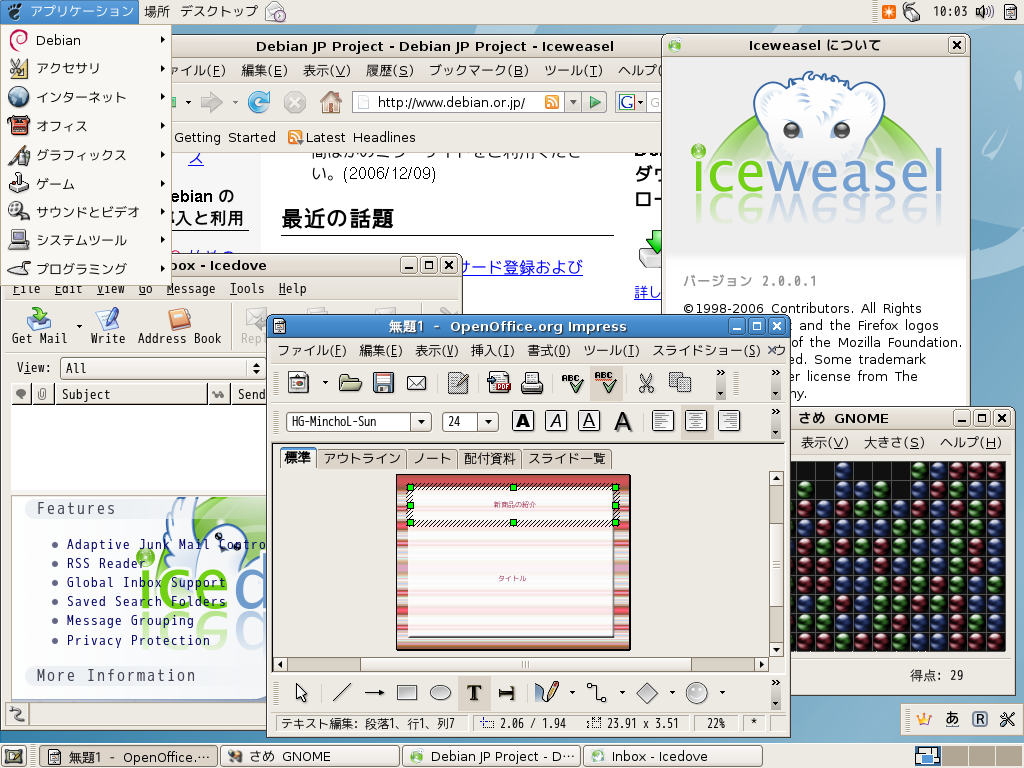
\includegraphics[width=5cm]{image201004/gnome.png}
        \caption{lenny での Gnome の画面}
    \end{center}
\end{wrapfigure}
\index{gnome}
GNOME は GUI ツールキットに GTK+ を使用した統合デスクトップ環境です。
Lenny に収録されているのは 2.22、
現在 squeeze に収録されているのは 2.30 です。(2010年7月現在)

Linux において「統合デスクトップ環境」という単語が目立ち始めた時から KDE(後述)と双璧をなして発展してきました。
現在では「統合デスクトップ環境」と言えば、この GNOME か KDE(後述)と言って良いくらい流行っています。
Debian ではインストーラで GUI インストールを選択すると GNOME のデスクトップ環境が導入されます。
また、Ubuntu でも標準で採用されているため馴染のある人も多いかもしれません。

GNOME をインストールするには、タスクから「Gnome デスクトップ環境」を選ぶか、導入したいパッケージの量に合わせて
\begin{description}
      \item[gnome] 
    GNOME 環境全て(GNOME プロジェクトが配布していない物も含める)
      \item[gnome-desktop-enviornment]
    GNOME プロジェクトの公式配布物としてのGNOME 関連のパッケージ全て
      \item[gnome-accessibility]
    必要最小限のパッケージにスクリーンリーダなどの小物を加えた環境
      \item[gnome-core]
    必要最小限の環境。アプリケーションは別途導入する必要がある
\end{description}
等のメタパッケージをインストールします。

その他、DebianでのGNOMEについては、Debian GNOME Packaging に情報が集まっているので参考にするとよいでしょう。

\begin{itemize}
 \item Debian GNOME Packaging

       \url{http://pkg-gnome.alioth.debian.org/}

\end{itemize}


\subsubsection{KDE -- the K Desktop Environment}
\begin{wrapfigure}{r}{5.5cm}
 \begin{center}
  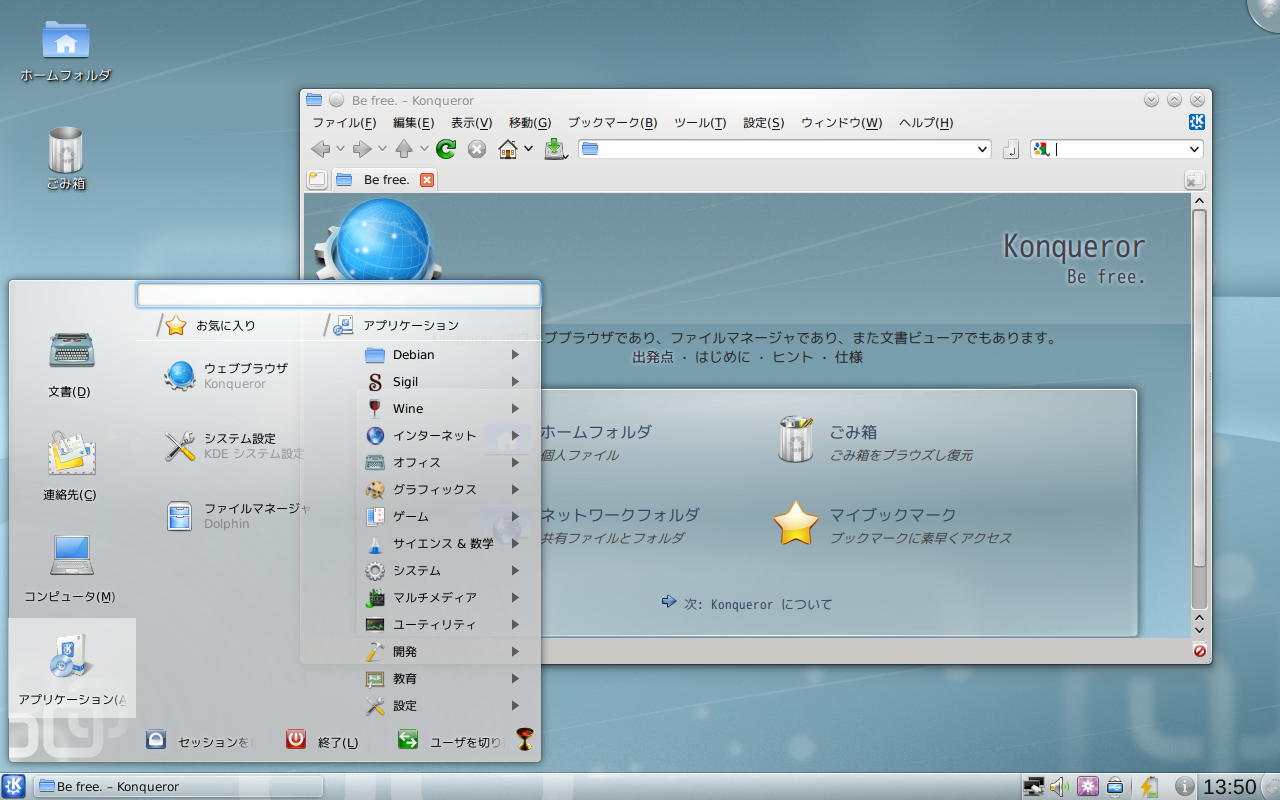
\includegraphics[width=5cm]{image201004/kde44.png}
  \caption{KDE 4.4の画面}
 \end{center}
\end{wrapfigure}
\index{kde}

KDEは、GUIツールキットにQt(キュート)を利用した統合デスクトップ環境で、
LennyではリリースのタイミングからKDE 3.5、squeeze/sidではKDE 4.4が収録さ
れています。(2010年7月現在)

KDE 3系とKDE 4系は、ツールキットがQt3とQt4が違うほか、機能やデスクトップ
自体の考え方まで変わっているのでKDE 3系が好きだった人はとまどうかもしれま
せん。

KDEをインストールするには、タスクから「KDE デスクトップ環境」を選ぶか、
導入したいパッケージの量に合わせて
\begin{description}
      \item[kde]
    KDE 環境全て(KDE プロジェクトが配布していない物も含める)
      \item[kde-core]
    必要最小限の環境。アプリケーションは別途導入する必要がある
\end{description}
等のメタパッケージをインストールします。

その他、DebianでのKDEについては、Debian KDE Maintainersのサイトに情報が集
まっているので参考にするとよいでしょう。

\begin{itemize}
 \item The Debian KDE maintainers website:

       \url{http://pkg-kde.alioth.debian.org/}

\end{itemize}

\subsubsection{Xfce4}
\begin{wrapfigure}{r}{5.5cm}
 \begin{center}
  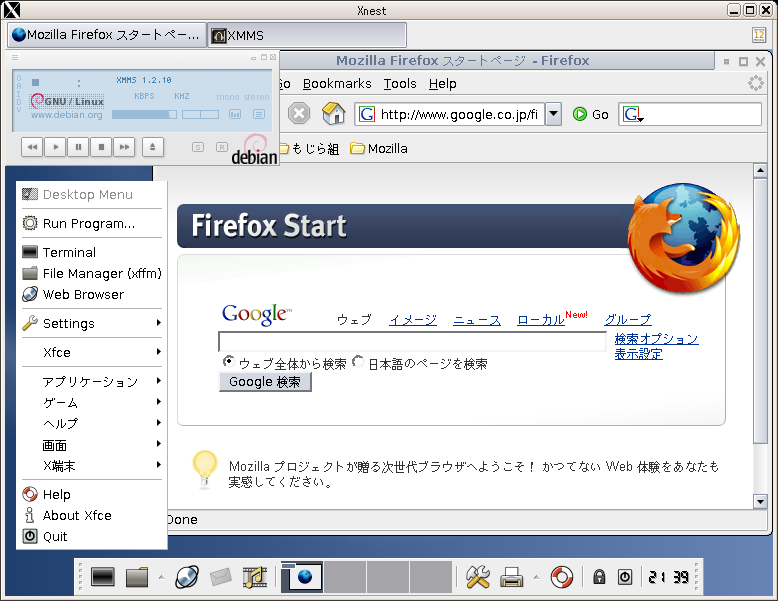
\includegraphics[width=5cm]{image201004/xfce4.png}
  \caption{Xfce4 の画面}
 \end{center}
\end{wrapfigure}
\index{xfce4}

GNOME や KDE はそれなりにメモリを必要としますし、それなりに重いです。
そこで X で利用できる軽量なデスクトップ環境の構築を目標として作成されたの
がXfce です。名前の由来は {\it XForms Common Environment} です。バージョ
ン3 までは GUI ツールキットとして XForms を使用し、商用 UNIX の
CDE(Common Desktop Environment)を模していましたが、バージョン4 以降はGUI
ツールキットとして GTK+2 を使用し、それまでと雰囲気ががらりと変わりました
(そんな訳で バージョン4 以降を強調するために Xfce{\bf{4}} と呼ぶ事も多い
です) 。

同じ GTK+ を使用している GNOME と比較して(見た目も綺麗な割に)非常に軽量に
動作するのが特徴です。また、プロジェクトの公式配布物ではないものの、Xfce
Goodies と呼ばれるプラグインが続々と開発されており、非常に使い易い環境と
なっています。

Xfce4 をインストールするには、タスクから「Xfce デスクトップ環境」を選ぶか、
{\tt xfce4} パッケージおよび {\tt xfce4-goodies}パッケージをインストールします。

その他、Debianにおける Xfce に関する情報は Debian Xfce Group のサイトに情報が集
まっているので参考にするとよいでしょう。

\begin{itemize}
 \item Debian Xfce Group:

       \url{http://pkg-xfce.alioth.debian.org/}

\end{itemize}



\subsubsection{LXDE}
\begin{wrapfigure}{l}{5.5cm}
 \begin{center}
  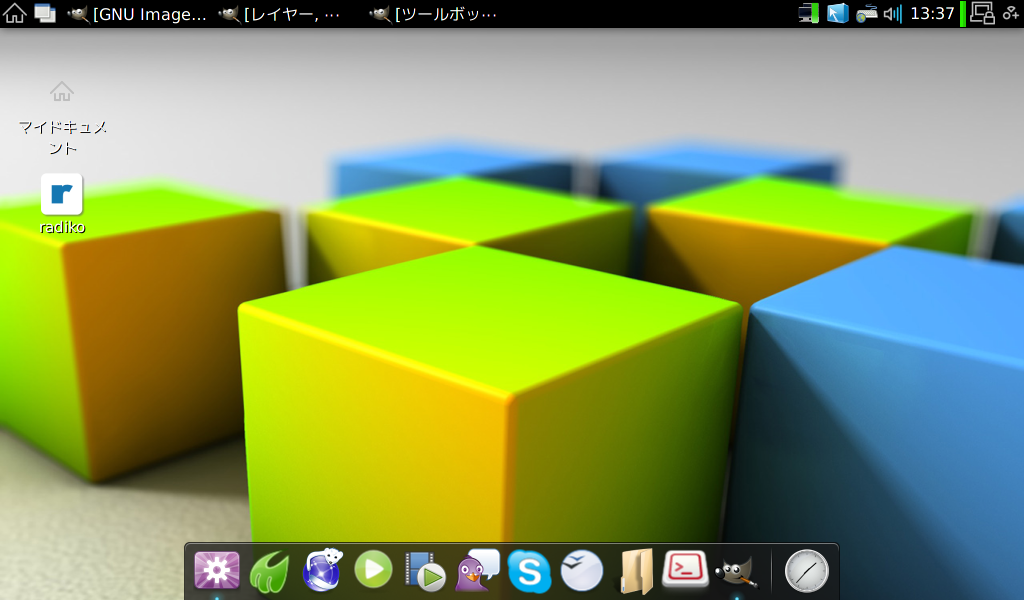
\includegraphics[width=5cm]{image201004/lxde-eeepc.png}
  \caption{LXDEをeeePCで利用している画面(ランチャーはGNOME Do)}
 \end{center}
\end{wrapfigure}
\index{lxde}

LXDEは初期起動時のメモリ使用量が100MBほどの軽量なデスクトップ環境です。

LXDEはGNOMEやKDE、Xfce4などの他のデスクトップ環境と比較すると、統合デスク
トップ環境としての共通ライブラリなどがなく、ウィンドウマネージャに
OpenBox、ファイルマネージャにPCManFM、パネルにlxpanelなど軽量のアプリケー
ションを組み合わせ、ゆるやかな形として統合デスクトップ環境を実現していま
す。

DebianでのLXDEパッケージはAndrew Leeさんが管理しています。

インストールについてはKDEと同様、lxdeというメタパッケージが用意されている
ので、aptitudeで容易にインストールできます。
\\
\begin{commandline}
$ sudo aptitude install lxde
\end{commandline}

LXDEは最新版がsqueezeに取り込まれる予定です。

% from debianmeetingresume201005-kansai.tex
\dancersection{次期リリースの squeeze を見てみよう}{のがたじゅん}
\index{squeeze}

\subsection{はじめに}
Debianな人なら知ってることも改めて解説しながら、次期リリース予定の
squeezeについて {\bf 2010年5月時点} の状況を解説します。

\subsection{squeezeって何?}
squeezeとは次期リリース予定のDebian安定版の開発コードネームです。バージョ
ン番号は6.0です。Debianの開発コードネームは、映画Toy Storyのキャラクター
名から取られ、squeezeは3つ目のエイリアンです。

\subsection{いつリリースなの?}
\label{sec:when-release-squeeze}

2009年7月に開催されたDebConf 9でリリースをタイムベース(時間で区切って)の
リリースに移行することが発表されました。
\footnote{\url{http://lists.debian.org/debian-announce/2009/msg00009.html}}
それによると12月フリーズ(新規機能などの追加停止)、翌年2010年3月にリリース
の予定でした。

しかし現安定版のLennyは、2009年2月にリリースされ、まだ一年も経っていない
状況では早すぎるとの判断から、改めて2010年3月にフリーズに入る予定でした。
\footnote{\url{http://lists.debian.org/debian-devel-announce/2009/10/msg00002.html}}

が、また一転。3月にネットワーク障害が起こったため、また仕切り直しになりフ
リーズは5月末から6月上旬に延期され
\footnote{\url{http://lists.debian.org/debian-devel-announce/2010/04/msg00001.html}}
リリースは未定になっています。

\subsection{squeezeのリリースゴール}
squeezeのリリース目標ですが、現在のところ2009年に発表されたリリースゴール
から変わっていません。以下、Debianニュースの「Debian GNU/Linux 6.0
"squeeze" リリースの目標」からの引用です。
\footnote{\url{http://www.debian.org/News/2009/20090730}}

\begin{itemize}
 \item 多数のアーキテクチャサポートによる、64 ビットマシンへの 32 ビット
       パッケージのインストール事情の改善
 \item kFreeBSD サポート、Debian 初の non-linux アーキテクチャの導入
 \item dash を新しいデフォルトシェルとしてブート性能を改善し、 依存ベース
       のブートシステムによるブートプロセスのクリーンアップと 並行処理に
       よる性能向上を図る
 \item 品質保証 (QA) プロセスをさらに拡張してパッケージの品質向上につなげ
       る。その内容:
        \begin{itemize}
         \item 全パッケージについてクリーンインストール、アップグレード及
               び削除
         \item 基礎的な品質チェックに通らなかったパッケージの自動拒否
         \item ダブルコンパイルのサポート
        \end{itemize}
 \item 新しいパッケージ形式を策定して、 将来の開発の能率化と圧縮アルゴリ
       ズムの改善を図る
 \item 旧式のライブラリを削除してセキュリティを改善
 \item ipv6 の完全サポート
 \item ラージファイルのサポート
 \item アーカイブ全体の debug パッケージの自動生成。Google Summer of
       Code プロジェクトのインフラへの統合を保留しています。
 \item パッケージの長い説明を\"翻訳済みパッケージリスト\"に分離して翻訳を
       促進し、 また、組み込みシステム向けに小さくしたフットプリントを提
       供します。 小さくなった Packages ファイルに感謝します。
 \item パッケージに複数の属性をタグ付けするシステム、debtags の統合の改善
       によってパッケージ選択をもっと簡単に
 \item メンテナによりアップロードされたバイナリパッケージを破棄、再ビルド
       し、 制御下の環境でビルドされたパッケージだけを残す
\end{itemize}

\subsection{今、やることは?}

まだ(2010年5月現在)フリーズになってません。\footnote{2010年6月に2010年8月
下旬フリーズ予定と発表されました。
\url{http://lists.debian.org/debian-devel-announce/2010/06/msg00002.html}}
変更点があってもまだ間に合います。(といっても大幅な変更は「5月21日までに
連絡を」と言っていたので難しいかもしれませんが、相談することが重要だと思
います。)それまでにRelease Critical Bug(リリースに障害となるバグ)を潰すこ
と、翻訳を進めるなど、いろいろあります。

\subsection{日本語関連で注意しなければいけないこと}

まずDefomaを使わなくなったことによる影響があげられます。

DebianにはDefoma(Debian Font Manager)というフォントを独自で管理する仕組
みがありますが、現在メンテナンスされておらず外されることが決定しました。

デスクトップ環境ではFontconfigによるフォント管理があるのでDefomaが外さ
れても影響はありませんが、TeX環境、特に日本語TeX環境についてはDefomaに
機能を依存していたこともあり影響が出ることが確認されています。

日本語TeX環境での影響は、GhostScriptで日本語PostScriptが扱えない、
dvipsk-jaがビルドできない/使えないなどあります。

TeX以外では日本語manではmanの整形をするroff(groff)が日本語の文字に中途
半端な対応のため、きちんと整形して表示されないなどの問題が確認されてい
ます。

これらの問題について、先日、対応するテストパッケージとDebian JPのアナウン
スが出たので、ご協力いただける方はアナウンスを読んで、Debian JP Devel ML
で反応してください。
\footnote{\url{http://lists.debian.or.jp/debian-announce/201005/msg00003.html}}

また、問題ではありませんが、武藤さんよりuimからIBusへの変更の提案が
Debian JP Devel ML出されていて、意見を求めているので、関心のある方はご意
見などをお寄せください。
\footnote{\url{http://lists.debian.or.jp/debian-devel/201005/msg00006.html}}

(2010年7月追記): TeX周りは佐々木さん、武藤さんらによって、ほぼ解消されま
した。IBusの変更についてはuimが継続となり、議論はsqueezeリリース後に持ち
越しになりました。

% =======================================================================
% from debianmeetingresume201002.tex
\dancersection{ブート方法が変わるよ}{まえだこうへい}
\index{upstart}
\index{sysvinit}
% =======================================================================

\subsection{squeeze からブート方法が変わる}
Debian のブートの仕組みには、System-V 系 Unix では伝統的な init
(sysvinit) が使われています。Debian の次期安定版6.0 (コードネーム
Squeeze) から、これが upstart に変わる予定です。今年の 3 月にフリーズ予
定、8月にリリース予定のSqueeze での予習の意味を込めて\footnote{今回も予
定通り遅れています。遅れた理由は\ref{sec:when-release-squeeze}「次期リリー
スのSqueezeを見てみよう」の「いつリリースなの?」を参照。}、今回はこの
upstart に変わることになった背景、init との比較を含めた upstart の仕組み、
実際に切り替え方法について説明します。

\subsubsection{背景}

upstart は、Debian をベースとしたディストリビューションであるUbuntu で、独
自に sysvinit の後継の仕組みとして開発されました。元々 sysvinit は伝統的
で安定した仕組みではありますが、現在使われているハードウェアで使うには機
能面、性能面から問題が出てきています。そこで、sysvinit の後継の仕組みと
して、upstart 以外にも複数のブートプロセスの仕組みが開発されています。し
かし、Ubuntu 以外にも Fedora 、また Google の Chrome OS, Chromium OS で
も upstart が採用されています。Debian でも squeeze から採用される予定と
いうこともあり、sysvinit の後継は upstart に落ち着く可能性が高いのではな
いでしょうか。

\subsubsection{そもそも init って何よ?}

upstart の話をする前に、init って何?という人向けにまず説明しましょう。
init は今更説明しなくても知っとるがな、という読者は、先に読み進めてくだ
さい。

init は Unix/Linux システムにおいて、カーネルがブートした後、ユーザプロ
グラムが起動するための仕組みです。例えば、あなたの使っているノート PC や
サーバに入っている Debian システムでもこの仕組みが必ず入っています。マシ
ンに電源を入れてから、ログイン画面が表示されるまでの流れは大まかには
\fgref{fig:upstart-sysvinit-bootimage}(ブートの流れ)のようになります。

\begin{figure}[H]
\begin{center}
\includegraphics[height=0.5\hsize]{image201002/sysvinit.eps}
\caption{ブートの流れ}
\label{fig:upstart-sysvinit-bootimage}
\end{center}
\end{figure}

init プロセスが起動すると、init は /etc/inittab の内容に従って、プロセス
のを生成や停止を行います。inittab の書式は次のようになります。

\begin{commandline}
id:runlevels:action:process
\end{commandline}

Debian システムのデフォルトランレベルは 2 なので、プロセスの生成に関わる
基本的なエントリは次の4行です。

\begin{commandline}
id:2:initdefault:                     ←デフォルトランレベルは2
si::sysinit:/etc/init.d/rcS           ←起動時は必ず実行
l2:2:wait:/etc/init.d/rc 2            ←ランレベル 2で実行。
1:2345:respawn:/sbin/getty 38400 tty1 ← getty を常駐
\end{commandline}

一行目(idがsi)にランレベルの指定が無いのは、action に sysinit が指定されているた
めです。これはステムブート中に実行され、他のブート用の action よりも優先
して実行されます。/etc/init.d/rcS の中では

\begin{commandline}
exec /etc/init.d/rc S
\end{commandline}

だけが実行されます。このワンライナーは /etc/init.d/rc でのブート用の変数を設定します。
この後、上記の rc スクリプトに対し、起動時に指定するランレベルを引数と
して実行されますが、Debian でのデフォルトランレベルは2です。

\begin{commandline}
id:2:initdefault:
\end{commandline}

ですので、実際には下記が実行されます。

\begin{commandline}
l2:2:wait:/etc/init.d/rc 2
\end{commandline}

とだけが実行されます。これはランレベル S のシングルユーザモードのときのも
のです。上記3行目でランレベル 2のときに実行されるエントリがあることから
も分かるとおり、
\begin{enumerate}
 \item ランレベル Sのプロセスが実行
 \item ランレベル 2のプロセスが実行
\end{enumerate}
の順で起動プロセスが実行されます。ランレベル S 用の起動処理が終わってか
ら、ランレベル 2 用の起動処理が実行されるのですから、/etc/rcS.d/ 以下と
/etc/rc2.d/ 以下を比較しても分かるとおり、これが逐次実行されるのはかなり
時間がかかるでしょう。ただし、同じレベルのスクリプトは並行して実行される
ように改善はされています。

\begin{commandline}
# Now run the START scripts for this runlevel.
# Run all scripts with the same level in parallel
CURLEVEL=""
for s in /etc/rc$runlevel.d/S*
do
        # Extract order value from symlink
        level=${s#/etc/rc$runlevel.d/S}
        level=${level%%[a-zA-Z]*}
        if [ "$level" = "$CURLEVEL" ]
        then
                continue
        fi
        CURLEVEL=$level
        SCRIPTS=""
        for i in /etc/rc$runlevel.d/S$level*
        do
                [ ! -f $i ] && continue

                suffix=${i#/etc/rc$runlevel.d/S[0-9][0-9]}
(snip)
                SCRIPTS="$SCRIPTS $i"
                if is_splash_stop_scripts "$suffix" ; then
                        $debug splash_stop || true
                fi
        done
        startup $ACTION $SCRIPTS
done
\end{commandline}

起動スクリプトの起動以外には、ランレベル 2 から 5 または、2 か 3 の時に
はコンソールから getty が実行されます。action が \texttt{respawn} となっ
ていますが、これは getty プログラムが終了したら、init が再起動させるため
の指示です。あるユーザがコンソールからログインしたセッションを、ログアウ
トすると getty は終了しますが、init により再び ログイン画面で待ち受ける
ことができる、というわけです。

\begin{commandline}
1:2345:respawn:/sbin/getty 38400 tty1
2:23:respawn:/sbin/getty 38400 tty2
3:23:respawn:/sbin/getty 38400 tty3
4:23:respawn:/sbin/getty 38400 tty4
5:23:respawn:/sbin/getty 38400 tty5
6:23:respawn:/sbin/getty 38400 tty6
\end{commandline}

init の他の役割としては、システム停止時のプロセスの停止にも関わっていま
す。

\subsection{upstart とは}

それでは、init についての予備知識を得たところで、本題の upstart に入りま
しょう。upstart は sysvinit をイベントベースに置き換えたもので、
サービスの開始と停止はイベントの通信にもとづきます。upstart の主な特徴は
次の 6 つです。

\begin{itemize}
 \item イベントドリブンでタスクやサービスを起動・停止する。
 \item タスクやサービスが起動・停止することでイベントが発生する。
 \item イベントはシステム上の他のプロセスから受け取ることができる。
 \item サービスが予期せず突然終了しても再起動することができる。
 \item デーモンの監視と再起動は親プロセスから分離できる。
 \item D-Bus を通じて init デーモンと通信できる。
\end{itemize}

upstartは、sysvinitと同様な機能を提供しますが、\textbf{非同期イベントに
応じて自律的に動作する点}がもっとも異なります。そのため、sysvinit に対す
る upstart のメリットには、
\begin{itemize}
 \item 利用可能なハードウェアだけでブートするため、runlevel が必要ない。
       これは存在しないハードウェアを必要とするジョブをトリガーとしない
       ため。
 \item ホットプラグデバイスに対応
\end{itemize}
といったことが挙げられます。

例えば、システムがブート後、NICを挿すと
\begin{enumerate}
 \item network-interface-add イベント生成
 \item DHCPジョブがネットワークカードを構成
 \item network-interface-upイベントが生成
 \item デフォルトルートが新しいインタフェースに割り当て
 \item default-route-upイベントが生成
 \item NICを必要とするジョブ(各種サーバ)が自動的に開始される
\end{enumerate}
という動きをします。逆にネットワークカードがなくなった場合は自動的に停止されます。

ただし、現在、squeeze/sidで採用されている upstart は、sysvinit の互換モー
ドのものです。upstart の最終目標は、イベントドリブンのブートプロセスに完
全に移行することですが、互換モードでは、sysvinit の動作を模倣しています。
\footnote{なお、Ubuntu 9.10 以降では ネイティブモードに移行しているよう
です。}

upstart の状態遷移は\fgref{fig:upstart-stats}のようになります。\footnote{upstart のドキュメ
ントに付属のものを掲載。}

\begin{figure}[h]
\begin{center}
\includegraphics[height=0.7\hsize]{image201002/states.eps}
\caption{upstart 状態遷移}
\label{fig:upstart-stats}
\end{center}
\end{figure}

\subsubsection{sysvinit と変わらない点}
\label{se:same-sysvinit}

Debian の upstart は、前述のとおり、Debian システムの起動・停止という重要な部分の
置き換えを行うため互換モードのものが採用されています、下記は sysvinit と
仕様上の変更がない部分です。\footnote{なお、\ref{se:same-sysvinit}「sysvinitと変わらない点」と\ref{se:difference-sysvinit}「sysvinitと違う点」は upstart パッケージの README.Debian.gz に記載されている FAQ をまとめ直したものです。}

\begin{itemize}
 \item initscript がインストールされる場所。パスは /etc/init.d/。
 \item 起動・停止用の initscript 。/etc/init.d/以下から /etc/rc?.d/
       以下に symlink が張られる。
 \item 起動・停止用 initscript の順序。SNNname, KNNname として symlink
       を張る。NN は00から99。Kスクリプトが最初に序数順に実行され、Sスク
       リプトがそのあと実行される。
 \item 現在および一つ前のランレベルを確認する方法。\texttt{runlevel} コ
       マンドを使う。
 \item ランレベルの変更方法。\texttt{telinit} コマンドか \texttt{init}
       コマンドを実行する。
 \item デフォルトのランレベルの変更方法。/etc/inittab ファイルの
       \texttt{id:N:initdefault:}のNを書き換える。
 \item シャットダウンの方法。upstart パッケージで提供される、
       \texttt{shutdown}コマンドや \texttt{reboot}, \texttt{halt},
       \texttt{poweroff}といったショートカットを使う。コンソールで
       Control-Alt-Delete を押してリブート出来る点も同じ。
\item シングルユーザモードにする方法。GRUB から\textbf{(recoveryode)}オ
      プションを選択か、カーネルのコマンドラインで、\texttt{-s, S,
      single}などの引数を指定する。稼働中のマシンでは、\texttt{telinit
      1} か \texttt{shutdown now}コマンドを実行する。
\end{itemize}

\subsubsection{sysvinit と違う点}
\label{se:difference-sysvinit}

互換モードでも全てが sysvinit と動作が同じというわけではなく、upstart の
固有の部分もあります。主に getty 関連の設定が変わる点が大きな違いです。

\begin{itemize}
 \item Control-Alt-Delete による挙動の変更方法。
       /etc/init/control-alt-delete.confの\textbf{exec}で始まる行を変更
       する。キーを押しても何も実行されないようにするには、ファイルを削
       除するだけ。
\begin{commandline}
(snip)
start on control-alt-delete

task
exec shutdown -r now "Control-Alt-Delete pressed"
\end{commandline}
 \item getty を常駐させる数を減らす方法。/etc/init/ttyN.conf ファイ
       ルを変更する\footnote{\textbf{N}は1から6の数字}。必要なければファ
       イル自体を削除する。
 \item getty の設定変更の反映方法。ファイルを変更したり削除してもすぐには
       反映されない。\\
       停止は\texttt{stop ttyN}コマンドを、起動は\texttt{start ttyN}コマンドを実行する。
 \item getty のパラメータの変更方法。/etc/init/ttyN.conf の
       \textbf{respawn}で始まる行を変更する。
\begin{commandline}
# tty1 - getty
#
# This service maintains a getty on tty1 from the point the system is
# started until it is shut down again.

description     "Start getty on tty1"
author          "Scott James Remnant <scott@netsplit.com>"

start on stopped rc RUNLEVEL=[2345]
stop on runlevel [!2345]

respawn
exec /sbin/getty 38400 tty1
\end{commandline}
 \item getty を実行するランレベルの変更方法。/etc/init/ttyN.conf の次
       の2行を変更する。\\
       stop の\textbf{!} は否定で、start と stopの設定は、\textbf{!}以外
       は基本同じにする。
 \item getty の数を増やす方法。/etc/init/ttyN.confを、ttyS0などの名前でコ
       ピーする。\textbf{respawn}の行に必要な設定をを記述する。
 \item シリアルコンソールを追加する場合は、上記の''getty の数を増やす方法''と同じ。
 \item upstart が動かない場合のデバッグ方法。カーネルコマンドラインに
       \texttt{--debug}オプションをつけ、\texttt{quiet} と
       \texttt{splash} オプションがある場合はそれらを削除する。upstart
       が実行されるとデバッグメッセージが出力される。
       \footnote{initramfs-tools ではなく initramfs 生成ツールを使ってい
       る場合にはこのオプションを使うと既知のバグもあるので気をつけましょう。}。
 \item upstart が動かない場合のシステム復旧手順。
 \begin{enumerate}
  \item カーネルコマンドラインから、\texttt{quite}と\texttt{splash}があれば削除し、
	\texttt{init=/bin/bash}を引数として起動すると、root shellが起動
	される。
  \item /etc/init.d/rcS を実行して、ハードウェアやネットワークの基本設定
	を行う。
  \item upstart がちゃんとインストールされているか確認する。/etc/initディ
	レクトリに全てのファイルがインストールされているかチェックし、正
	常にインストールされてない場合は upstart パッケージを再インストー
	ルする。
  \item /etc/init にファイルが今度はちゃんとあるか確認する。
  \item \texttt{sync}と\texttt{reboot -f}コマンドを実行し、マシンを再起動
	する。
 \end{enumerate}
 \item upstart ジョブリストをクエリする方法。\texttt{initctl list}コマ
       ンドでジョブとステータスを表示する。
\begin{commandline}
$ sudo initctl list
tty4 start/running, process 25474
rc stop/waiting
tty5 start/running, process 25478
control-alt-delete stop/waiting
rcS stop/waiting
rc-sysinit stop/waiting
dbus-reconnect stop/waiting
tty2 start/running, process 25473
tty3 start/running, process 25475
tty1 start/running, process 25477
tty6 start/running, process 25476
\end{commandline}
 \item ジョブの起動・停止方法。\texttt{start JOB}, \texttt{stop JOB}
       コマンドを実行する。
 \item ジョブのステータス表示方法。\texttt{status JOB}コマンド。
\begin{commandline}
$ sudo status tty1
tty1 start/running, process 25477
\end{commandline}
 \item 手動でイベントを発行する方法。\texttt{initctl emit EVENT}コマンド
       で名前付きイベントを発行し、待機中のジョブが状況に応じて起動 or
       停止する。
\end{itemize}

\subsection{upstart への切り替え}

それでは、早速 sysvinit から upstart へ切り替えてみましょう。
squeeze/sid と Lenny との場合を見てみます。

\subsubsection{squeeze/sid での場合}

squeeze/sid での upstart への切り替えには、upstart パッケージをインストー
ルします。通常のパッケージのインストールとは異なり、続行する場合は、
\textbf{Yes, do as I say}と入力しなさい、というメッセージが表示されます。
これは入れ替えは非常にリスクが高いためです。

\begin{commandline}
$ sudo apt-get install upstart
パッケージリストを読み込んでいます... 完了
依存関係ツリーを作成しています                
状態情報を読み取っています... 完了
以下の特別パッケージがインストールされます:
  dbus libdbus-1-3 libexpat1
提案パッケージ:
  dbus-x11
以下のパッケージは「削除」されます:
  sysvinit
以下のパッケージが新たにインストールされます:
  dbus libdbus-1-3 libexpat1 upstart
警告: 以下の不可欠パッケージが削除されます。
何をしようとしているか本当にわかっていない場合は、実行してはいけません!
  sysvinit
アップグレード: 0 個、新規インストール: 4 個、削除: 1 個、保留: 9 個。
1,005kB のアーカイブを取得する必要があります。
この操作後に追加で 2,105kB のディスク容量が消費されます。
重大な問題を引き起こす可能性のあることをしようとしています。
続行するには、'Yes, do as I say!' というフレーズをタイプしてください。
 ?] Yes, do as I say!
\end{commandline}

lxc の環境で試してみましたが、getty がうまく動かず、起動しては突然
死して、再起動されて、また突然死、というのを繰り返してしまうので、コンソー
ルからのログインは出来ない状態でしたが\footnote{2010年2月9日現在}、
\ref{ch:re-startup-upstart}「upstart再入門」でKVMの環境下で試した際には正常
に起動することを確認済みです。

\begin{commandline}
$ sudo lxc-start -n bootsid
cat: /proc/cmdline: No such file or directory
Setting the system clock.
Cannot access the Hardware Clock via any known method.
Use the --debug option to see the details of our search for an access method.
Unable to set System Clock to: Tue Feb 9 14:16:26 UTC 2010 ... (warning).
Activating swap...done.
mount: you must specify the filesystem type
Cannot check root file system because it is not mounted read-only. ... failed!
Setting the system clock.
Cannot access the Hardware Clock via any known method.
Use the --debug option to see the details of our search for an access method.
Unable to set System Clock to: Tue Feb 9 14:16:27 UTC 2010 ... (warning).
Cleaning up ifupdown....
Checking file systems...fsck from util-linux-ng 2.16.2
done.
Setting up networking....
Mounting local filesystems...done.
Activating swapfile swap...done.
Cleaning up temporary files....
Configuring network interfaces...done.
Setting kernel variables ...done.
Cleaning up temporary files....
Starting system message bus: dbus.
Starting OpenBSD Secure Shell server: sshd.
init: tty4 main process (239) terminated with status 1
init: tty4 main process ended, respawning
init: tty5 main process (241) terminated with status 1
init: tty5 main process ended, respawning
init: tty2 main process (242) terminated with status 1
init: tty2 main process ended, respawning
init: tty3 main process (244) terminated with status 1
init: tty3 main process ended, respawning
init: tty6 main process (245) terminated with status 1
init: tty6 main process ended, respawning
init: tty1 main process (306) terminated with status 1
init: tty1 main process ended, respawning
init: tty4 main process (307) terminated with status 1
init: tty4 main process ended, respawning
(snip)
\end{commandline}

この時も、ssh 経由のターミナルログインは問題なくできました。

\begin{commandline}
$ ssh bootsid
Enter passphrase for key '/home/user/.ssh/id_rsa': 
Linux bootsid 2.6.32 #1 SMP Mon Dec 7 05:27:50 UTC 2009 x86_64

The programs included with the Debian GNU/Linux system are free software;
the exact distribution terms for each program are described in the
individual files in /usr/share/doc/*/copyright.

Debian GNU/Linux comes with ABSOLUTELY NO WARRANTY, to the extent
permitted by applicable law.
Last login: Tue Feb  9 14:18:38 2010 from 192.168.189.114
user@bootsid:~$ 
\end{commandline}

\subsubsection{Lenny での場合}

squeeze/sid でもうまく行っていない状況ですので、squeeze が stable として
リリースされるときに、検討しましょう\footnote{upstart が予定どおり squeeze に含まれて
いることが前提ですが。}。あるいは、sid にアップグレードすることを検討し
ても良いでしょう。

\subsubsection{まとめ}

現時点では、実際に切り替わった際にはオペレーション上も多少変更があります。
Ubuntu 9.10 で採用されている ネイティブモードでは更にオペレーションも変
わるようですので、今回はじめて upstart を知ったという方は、次章も参考の
上、早めに使い方や仕組みを予習し、バグ出しに協力されるとDebianの品質も向
上することでしょう。


% from debianmeetingresume201004.tex
\dancersection{upstart 再入門}{まえだこうへい}

\subsection{はじめに}
\label{ch:re-startup-upstart}
今年の2月の Debian 勉強会(Debian 温泉)\footnote{本書では前章にあたり
ます。}で一度扱ったテーマです。今回は起動速度の観点から変化があるかを
見てみましょう。
\footnote{4月時点では、書き下ろすつもりでしたが、個人的な都合で余裕がな
く、今回の事前配布資料は基本的に、2010年2月の Debian 勉強会の資料「ブー
ト方法が変わるよ」を再編しただけだったので、起動速度の検証について当日発
表のみ行いました。}

\subsubsection{事前準備}
前章とは異なり、検証のための環境はKVMで用意し、起動速度の比較には
bootchartを用いました。
用意するインストールイメージと、パッケージは下記の通りです。

 \begin{itemize}
  \item debian-testing-amd64-businesscard.iso
  \item qemu-kvm パッケージ
  \item qcow2 フォーマットのディスクイメージ
  \item bootchart パッケージ
 \end{itemize}

KVM/QEMUゲストには、sysvinitとupstartの2種類を用意しました。
\begin{itemize}
 \item Debian GNU/Linux sid の最小構成をインストール
 \item インストール後、ディスクイメージからコピー作成
 \item コピー後、upstart パッケージをインストール
\end{itemize}

\subsubsection{upstartのインストール}

前章でも触れた部分ですが、再掲します。
切り替えには upstart パッケージをインストールします。通常のパッケージのインストールとは異なり、続行する場合は、\textbf{Yes, do as I say}と入力しなさい、というメッセージが表示されます。
これはうまくいかない場合は Debian システムが起動できなくなるなどのリスク
があるためです。

\begin{commandline}
$ sudo apt-get install upstart
パッケージリストを読み込んでいます... 完了
依存関係ツリーを作成しています                
状態情報を読み取っています... 完了
以下の特別パッケージがインストールされます:
  dbus libdbus-1-3 libexpat1
提案パッケージ:
  dbus-x11
以下のパッケージは「削除」されます:
  sysvinit
以下のパッケージが新たにインストールされます:
  dbus libdbus-1-3 libexpat1 upstart
警告: 以下の不可欠パッケージが削除されます。
何をしようとしているか本当にわかっていない場合は、実行してはいけません!
  sysvinit
アップグレード: 0 個、新規インストール: 4 個、削除: 1 個、保留: 9 個。
1,005kB のアーカイブを取得する必要があります。
この操作後に追加で 2,105kB のディスク容量が消費されます。
重大な問題を引き起こす可能性のあることをしようとしています。
続行するには、'Yes, do as I say!' というフレーズをタイプしてください。
 ?] Yes, do as I say!
\end{commandline}

2月の Debian 勉強会時点\footnote{本書では前章}では、lxc の環境で試した際
\footnote{2010年2月9日現在}は、getty がうまく動かず、起動しては突然死し
て、再起動されて、また突然死、というのを繰り返してしまい、コンソールから
のログインは出来ない状態でしたが、今回の資料作成時点\footnote{2010年4月
11日に、Squeeze Official Snapshot amd64 BC Binary-1 20100322-03:30の ISO イメージを使用した最小構成。}では、KVM環境で問題なく起動します。バージョンが変わってませんが、環境が異なる
ので原因は後者にありそうではあります。

\subsubsection{起動速度を比べてみる}
プロセスを並行処理させることで処理速度を向上させるので、プロセスが多いほ
ど、効果は高いはずではないか、とか考えられます。

比較のために用意した環境は以下の通りです。

\begin{itemize}
\item ブートの種類
\begin{itemize}
\item sysvinitとupstart
\end{itemize}
\item 構成
\begin{itemize}
\item 最小構成 baseにbootchartをインストール
\item CouchDB 最小構成にcouchdb をインストール
\item LAMP CouchDB の構成にapache2,rails, mysql-serverをインストール
\item GNOME 最小構成に xserver-xorg, gnome をインストール 
\end{itemize}
\end{itemize}

\newpage

\subsubsection{bootchartの結果}
\begin{figure}[thbp]
\subfigure[sysvinit]{\makebox[.45\linewidth][c]{
  \includegraphics[height=0.5\hsize]{image201004/upstart/sysvinit-bootchart.eps}}}
\subfigure[upstart]{\makebox[.45\linewidth][c]{
  \includegraphics[height=0.5\hsize]{image201004/upstart/upstart-bootchart.eps}}}
\caption{最小構成}
\end{figure}

\begin{figure}[thbp]
\subfigure[sysvinit]{\makebox[.45\linewidth][c]{
\includegraphics[height=0.5\hsize]{image201004/upstart/sysvinit-couchdb-bootchart.eps}}}
\subfigure[upstart]{\makebox[.45\linewidth][c]{
\includegraphics[height=0.5\hsize]{image201004/upstart/upstart-couchdb-bootchart.eps}}}
\caption{CouchDB}
\end{figure}

\begin{figure}[thbp]
\subfigure[sysvinit]{\makebox[.45\linewidth][c]{
\includegraphics[height=0.5\hsize]{image201004/upstart/sysvinit-lamp-bootchart.eps}}}
\subfigure[upstart]{\makebox[.45\linewidth][c]{
\includegraphics[height=0.5\hsize]{image201004/upstart/upstart-lamp-bootchart.eps}}}
\caption{LAMP}
\end{figure}

\begin{figure}[thbp]
\subfigure[sysvinit]{\makebox[.45\linewidth][c]{
\includegraphics[height=0.5\hsize]{image201004/upstart/sysvinit-desktop-bootchart.eps}}}
\subfigure[upstart]{\makebox[.45\linewidth][c]{
\includegraphics[height=0.5\hsize]{image201004/upstart/upstart-desktop-bootchart.eps}}}
\caption{GNOME}
\end{figure}

\clearpage
\subsubsection{結果}
起動速度調査結果を\tbref{tb:bootchart-check}に示します。

\begin{table}[H]
\begin{center}
\caption{起動速度調査結果}
\label{tb:bootchart-check}
\begin{tabular}{|c|c|c|c|c|}\hline
initの種類 & 最小構成&
 CouchDB & LAMP & GNOME \\
\hline\hline
sysvinit & 5 sec & 6 sec & 8 sec & 8 sec \\
\hline
upstart & 5 sec & 6 sec & 8 sec & 8 sec \\
\hline
\end{tabular}
\end{center}
\end{table}

起動時間にはまったく違いがありませんでした。が、本書を読んでいる読者の皆
さんは既にお気づきのはず。Debianのupstartは互換モードなので、sysvinitの
動作を模倣しているのでした。これでは比較になりませんね。

\subsection{Ubuntu 9.10を試してみた。}

そこで、Debianとは若干構成が変わりますが、ネイティブモードのupstartになっているUbuntu 9.10で試してみること
にしました(\fgref{fig:ubuntu-upstart-check})。違いとしては、以下のように
なりました。

\begin{itemize}
 \item init の処理終了時で bootchart のログ収集を止めるわけでは
       ないようだが、実質的には25秒程度で起動が完了。
 \item でも起動プロセスが並行処理されていること Debian での結果を比べて
       も分かります。
\end{itemize}

\begin{figure}[thbp]
\begin{center}
\includegraphics[height=0.6\hsize]{image201004/upstart/ubuntu-karmic-20100417-3.eps}
\caption{Ubuntu 9.10のupstart}
\label{fig:ubuntu-upstart-check}
\end{center}
\end{figure}

%\newpage

\subsection{まとめ}
ネイティブモードじゃないと upstart は本来のメリットが活かせない感じとい
うことが分かりました。とはいえ、いきなりネイティブモードの upstart に切
り替えるのはリスクあるので、一時的に互換モードを使うのは止むを得ないのか
もしれません。ただ、Squeeze でずっと互換モードなのもどうかと思います。
SqueezeAndAHalfリリース時(リリースされるなら、ですが)にネイティ
ブモードに切り替えられるとうれしいかもしれません。

結論としては、「みんなで試してバグ出ししましょう」というところです。

\subsection{参考資料}

\url{http://www.ibm.com/developerworks/jp/linux/library/l-boot-faster/index.html}
\clearpage

% from debianmeetingresume201001-kansai.tex
\dancersection{Xenで作る自宅サーバ}{川江 浩}
\index{xen}

\subsection{はじめに}
近年、CPUの性能がパワフルになるにつれて、高価なハードウェアを前提とした
仮想化技術がパーソナルベースでも使えるようになってきました。

そこで、脚光を浴びてきた仮想化技術の代表格であるXenを使って、インタネッ
ト関連のサーバ群を構築しましたので、DebianベースでXenの仮想サーバを構築
する時に注意することや、上記サーバ群を構築する際に思ったことをレポート
します。

また、以下の仕様はパーソナルベースでの運用を前提に構築したものです。仕
様を試そうとするときは、必ずデータ等のバックアップをとって自己責任で行っ
てください。より詳しく知りたい方は専門書を参照してください。

\subsection{Xenとは}
Xenは、仮想マシンソフトウェアの一つで、OSより1つの下の階層でハイパーバ
イザというプログラムを動かすものです。このタイプはハイパーバイザ型と呼
ばれ、「VMware Infrastrucure」などがあります。

他方、仮想マシンソフトウェアにはアプリケーションタイプと呼ばれるものが
あり、「VMware Workstation」「VirtualBox」「QEMU」が有名です。

\subsection{Xenの特徴}
Xenは仮想化するためのモデルとして、準仮想化と完全仮想化の2つを提供しています。
\begin{itemize}
\item 準仮想化(ParaVirtualization)\\
Xenでの準仮想化はハードウェアをエミュレートする代わりに、仮想マシン用のハードウェアを使用します。このハードウェアは操作をするためにハイパーバイザコールを呼び出します。ハイパーバイザコールは仮想マシン環境に対応し、OSはXen仮想ハードウェア用に修正する必要があります。

\item 完全仮想化(FullVirtualization)\\
Xenは完全仮想化機能も提供しています。この機能を利用すると、デフォルトのOSをそのままXen上で動作させることができます。
\end{itemize}

\subsection{Xenの形態}
XenはLinuxをベースに作られていますので、Xen用にコンパイルされたカーネルを利用します。このカーネルは起動時にハイパーバイザをロードし、その上にカーネルをロードします。イメージ的にはハイパーバイザ上を管理OSのDomainOが動き、そのOSに管理される形でゲストOSと呼ばれるDomainUが動きます。

\begin{itemize}
\item Domain-O (管理OS)以下DomO \\
      Xenを起動したOS。ハードウェアを管理し、ハイパーバイザ上で動作するゲストOSの管理を行う。
\item Domain-U (DomU-準仮想化)以下DomU \\
      Domain-Oによって起動、管理されるゲストOS。特に、準仮想化で動作する。
\item HVM Domain (HVM-完全仮想化)以下HVM \\
      Domain-Oによって起動、管理されるゲストOSであるが、完全仮想化であるHVM(Hardware Virtual Machine)で動作する。
\end{itemize}

%図形の挿入
\begin{figure*}[h!]
 \centering
 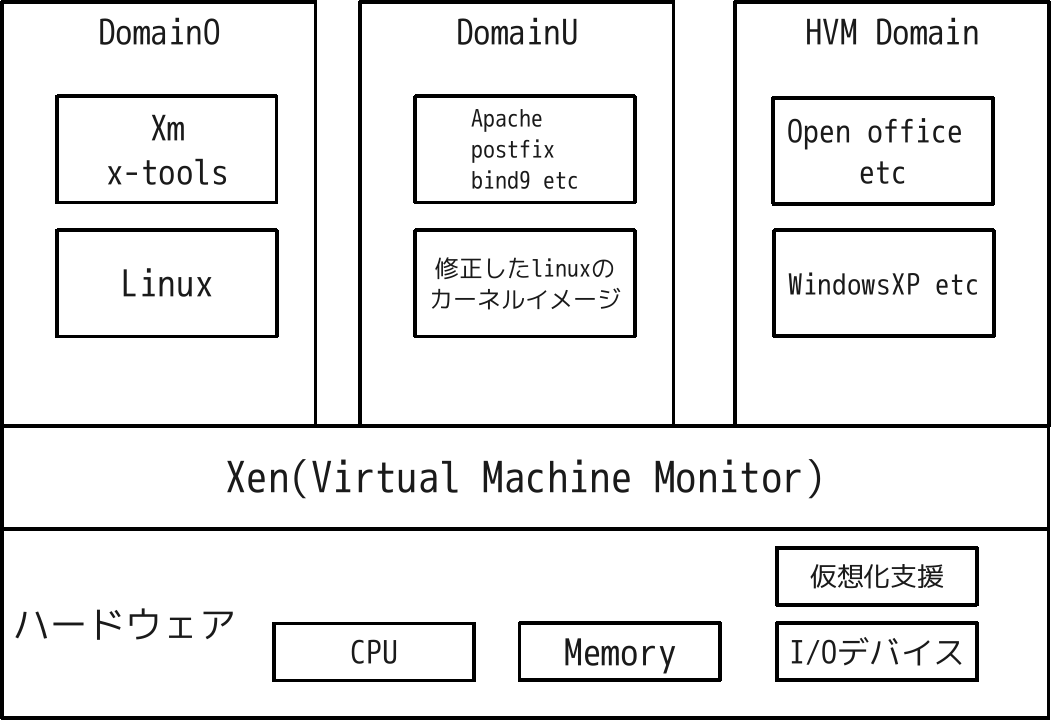
\includegraphics[scale=0.6]{image201001/xen-image.png}
 \caption{Xen のハイパーバイザモデルのイメージ}
\end{figure*}
\clearpage

\subsection{Xen の導入}
次に, Xen をインストールします. インストールは各アーキテクチャによって異なります. \footnote{詳しくは, 仮想化技術 Xen -概念と内部構造などを参照してください. 完全仮想化を目的にするのであれば Intel-VT や AMV-V が, CPU で仮想化支援機能を持っています. } ここでは, インテルをベースに Lenny の Xen カーネルイメージ 2.6.26 を以下の様にインストールします.

\begin{commandline}
# aptitude install xen-linux-system-2.6.26-2-xen-686 
\end{commandline}
また, Debian には DomU を作るツールも用意してありますので, これもインストールします.
\begin{commandline}
# aptitude install xen-tools
\end{commandline}
各インストールが済んだら, /xen/xen/xend-config.sxp ファイルの以下の箇所を変えます.
\begin{commandline}
(network-script 'network-bridge netdev=eth1')
(network-script 'network-bridge netdev=eth0')
\end{commandline}
再起動し, DomO の起動を確認します.
\begin{commandline}
# xm list
Name                 ID   Mem  VCPUs   State   Time (s)
Domain-0             0   1478     1   r-----    217.6
\end{commandline}

\subsection{DomU の設定}
Xen のツールを使ってゲスト OS を以下の手順で入れます. (etch や Ubuntu, CentOS も可能).
\begin{enumerate}
\item 設定ファイルの編集
\item xen-create-image の実行
\item DomU の起動
\end{enumerate}

\subsubsection{設定ファイルの編集}
設定ファイルは, /etc/xen-tools/xen-tools.conf です. 以下, DomU に Lenny をインストールものとして編集します.

%改ページ, 注意
\begin{commandline}
##
#  /etc/xen-tools/xen-tools.conf
##             (中略)
#  Output directory for storing loopback images.
#
#  If you choose to use loopback images, which are simple to manage but
# slower than LVM partitions, then specify a directory here and uncomment
# the line.
#
#  New instances will be stored in subdirectories named after their
# hostnames.
# 
##
dir = /home/xen (イメージファイルの保管場所です)
#              (中略)

##
#  Disk and Sizing options.
##
size   = 4Gb      # Disk image size.
#memory = 128Mb    # Memory size
memory = 384Mb    # Memory size
#swap   = 128Mb    # Swap size
swap   = 512Mb    # Swap size
# noswap = 1      # Don't use swap at all for the new system.
fs     = ext3     # use the EXT3 filesystem for the disk image.
#dist   = etch     # Default distribution to install.
dist   = lenny     # Default distribution to install.

#  Currently supported and tested distributions include:
#
# via Debootstrap:
#
#  Debian:
#   sid, sarge, etch, lenny.(他のディストリビューションの選択も可能)
#
#  Ubuntu:
#   edgy, feisty, dapper.
#
# via Rinse:
#   centos-4, centos-5.
#   fedora-core-4, fedora-core-5, fedora-core-6, fedora-core-7

##
# Networking setup values.
##
#
## Uncomment and adjust these network settings if you wish to give your
# new instances static IP addresses.
#
# gateway   = 192.168.1.1
gateway   = 192.168.0.1
# netmask   = 255.255.255.0
netmask   = 255.255.255.0
# broadcast = 192.168.1.255
broadcast = 192.168.0.255
#(ネットワークはご自由に)

#(以下はデフォルトにしました)
# Default kernel and ramdisk to use for the virtual servers
#
kernel      = /boot/vmlinuz-`uname -r`
initrd      = /boot/initrd.img-`uname -r`

#  The architecture to use when using debootstrap, rinse, or rpmstrap.
#
#  This is most useful on 64 bit host machines, for other systems it
# doesn't need to be used.
#
# arch=[i386|amd64]
#

# The default mirror for debootstrap to install Debian-derived distributions
#
mirror = http://ftp.jp.debian.org/debian/

#  If you're using the lenny or later version of the Xen guest kernel you will
# need to make sure that you use 'hvc0' for the guest serial device,
# and 'xvdX' instead of 'sdX' for serial devices.
#
#  You may specify the things to use here:
#
serial_device = hvc0 #default
# serial_device = tty1
#
disk_device = xvda #default
# disk_device = sda

#  Here we specify the output directory which the Xen configuration
# files will be written to, and the suffix to give them.
#
#  Historically xen-tools have created configuration files in /etc/xen,
# and given each file the name $hostname.cfg.  If you want to change
# that behaviour you may do so here.
#
# output    = /etc/xen
# extension = .cfg
#
\end{commandline}

\subsubsection{xen-create-image の実行}
次に, DomU のイメージを作ります. 同時に DomU に割り当てる IP アドレスをオプションで指定します. 例えば, アドレスを 192.168.0.2, ホストネームを dns とするなら以下のようにします.
\begin{commandline}
# xen-create-image --ip 192.168.0.2 --hostname dns
\end{commandline}
DomU の制作には, イメージディスクの大きさやネットワークの状況によって異なりますが, 自分の環境では 10G のイメージで 30 分ぐらいでした.

\subsubsection{DomU の起動}
無事に, インストールができたら起動して, 稼働状況を見てみましょう.
\footnote{Xen には管理用ツールとして「 xm 」などがあります. 詳しくは, Xen 徹底入門などを参照してください. }
\begin{commandline}
# xen create -c dns.cfg
# xm list
 Name                                        ID   Mem VCPUs      State   Time (s)
 Domain-0                                     0  1478     4     r-----    429.8
 dns                                          5   384     1     -b----     10.5
 mail                                         2   384     1     -b----    123.6
 www                                          4  1792     1     -b----     23.1
\end{commandline}
起動してくる画面は, 全くの初期状態でログインプロンプトしか出ません. root でログインしてパスワードとユーザを作成します.
\begin{commandline}
# passwd
# adduser ipv6waterstar
\end{commandline}
\subsubsection{バックアップ, 他}
また, DomU をデフォルトでインストールした場合, DomO の/home/xen/domain に各 DomU のドメインごとにメージファイルが置かれます. また, 設定ファイルは/etc/xen に  ".cfg"ファイルとして保存されます.

従って, 例えば何らかの設定ミスをして DomU が起動不能になっても, 上記のイメージと設定ファイルのバックアップがあれば, 各ディレクトリと設定ファイルをそのままコピーし直すだけで, 同じ環境の DomU を復元できます.

また, 管理用の DomO はセキュリティの関係からプロセス数が少ない方がいいのですが, 後述のように設定ファイルを多数, 作成する場合のことも考えると, GUI で操作ができるなどの利点から, gnome などをインストールすることを勧めます.


\subsection{Xen のネットワークの概要}
Xen は仮想インターフェイスをベースにしたネットワーク機能を持っています.

具体的には, DomU の各ホストを直接外部ネットワークに接続するブリッジ経由の接続. 仮想インターフェイスを通して, DomO のルーティングし, ネットワークインターフェイスに出力するブリッジを経由しない接続 (NAT 接続) の二つの形態があります.

ブリッジ経由の接続のイメージはハードウェア上に, DomO と複数の DomU の仮想 PC があって, それぞれが対等にネットワークハブで繋がっているような状態です.

今回は, 各 DomU サーバをインターネットサーバとして運用したいので, 仮想インターフェイスを使って直接, セグメントが異なる外部ネットワークに接続できるブリッジ経由の接続でネットワークを構成します.

DomU は仮想マシンを作成するときに, IP アドレスを割り当てたので特別な設定は必要ありません. 同時に, Mac アドレスも各仮想インターフェイスごとに自動的に割り当てられます.

また, IP アドレスを後から変更したいときなどは/etx/xen 以下の".cfg"ファイルを書き換えます.

例  dns.cfg
%改ページ  注意
\begin{commandline}
#
# Configuration file for the Xen instance www, created
# by xen-tools 3.9 on Tue Nov 17 10:35:03 2009.
#

#
#  Kernel + memory size
#
kernel      = '/boot/vmlinuz-2.6.26-2-xen-686'
ramdisk     = '/boot/initrd.img-2.6.26-2-xen-686'
memory      = '384'(メモリーの容量の変更も可能)

#
#  Disk device (s).
#
root        = '/dev/xvda2 ro'
disk        = [
                  'file:/home/xen/domains/www/swap.img,xvda1,w',
                  'file:/home/xen/domains/www/disk.img,xvda2,w',
              ]


#
#  Hostname
#
name        = 'dns'(ホスト名)

#
#  Networking
#
vif         = [ 'ip=192.168.0.2,mac=00:12:34:56:78:9A' ]
(アドレスの変更も可能ですが, DomU の interfaces を書き換えているときはそちらも書き換えてください)

#
#  Behaviour
#
on_poweroff = 'destroy'
on_reboot   = 'restart'
on_crash    = 'restart'
\end{commandline}

\subsubsection{各インターネットサーバの設定する前の注意事項}
次に, DNS, Mail サーバ, Web サーバのパッケージを, 各 DomU にインストールします.

インストールは, 仮想マシンでもノーマルのインストールと変わりません. ただ, Xen のネットワーク構成は独特の「癖」のようなものがあります. 以下, いくつか例を挙げます.
\begin{enumerate}
\item NTP を使った時間の設定 
\item SSH でのログイン
\item その他 
\end{enumerate}

\subsubsection{NTP を使った時間の設定}
DomU は Dom0 からのみ時刻を更新できるという Xen の仕様なので, Dom0 で時刻を合わせていれば, DomU も正確な時刻を得ることができます. ただ, DomU で ntpd や ntpdate を実行するのであれば, 時刻同期できないことがあります.

普通に DomU で時計を合わせるのであれば, Aisa/Tokyo に合わせることで日本時間にできます (デフォルトでは UTC).
\begin{commandline}
# dpkg-reconfigure tzdata
# date
  Tue Jan 24 15:00:00 JST 2010
\end{commandline}

また, DomU で NTP 等を使うのであれば, DomU の/etc/sysctl.conf に{\tt xen.independent\_wallclock=1}を加えて再起動してください.

\subsubsection{SSH でのログイン}
Xen で SSH を使って, ネットワーク越しにログインする場合も通常と同じでが, インストールしたばかりの DomU は何も入っていないので, そのままではエラーになります.

具体的には, まず DomU に SSH をインストールします (ポート番号の変更などはお好みで).
\begin{commandline}
# aptitude install ssh
\end{commandline}

次にローカルから SSH を使ってログインしようとしても, 以下のエラーがでます.
\begin{commandline}
$ ssh mail.kinsen.gr.jp
  ipv6waterstar@dns.kinsen.gr.jp's password: 
  PTY allocation request failed on channel 0
\end{commandline}

原因は, xen-tools を使った DomU の構築で「 udev をインストールしないため」に起こります. 従って, DomU に udev をインストールすることで解決します.
\begin{commandline}
# aptitude install udev
\end{commandline}

\subsubsection{その他}
その他, Xen でサーバを運用するときにいくつか気づいたものを挙げます.

まず, DomO と DomU がブリッジ経由で接続している場合, iptables で FORWARD を使うと DomU からネットワークに繋がらない現象が起こります (理由は不明).

また, 完全仮想化でゲスト OS を動かそうとするのであれば, CD をゲスト OS からマウントし, VNC などを立ち上げてインストールする必要があります (検証はしてませんので, 可能かどうかは不明).

詳しくは, 以下のドキュメント等を参照してください.
\begin{itemize}
\item \url{http://wiki.debian.org/Xen}
\end{itemize}

\subsection{各インターネットサーバの設定}
次に, 各インターネットサーバの設定の手順を説明します. ここでの環境は, グローバル IP アドレスが 1 つで, インターネットには電話会社から提供されているルータで外部ネットワークに, 繋がっていることを前提とします.

\subsubsection{DNS の概要}
DNS サーバはホスト名と IP アドレスを対応させたゾーンと呼ばれるファイルを持ち, ホスト名の検索に対して対応する IP アドレスを返します. また, ゾーンファイルの内容を他のサーバに転送します.

具体的に www.kinsen.gr.jp というホスト名に対応する IP アドレスを (再帰) 検索する場合, まず, jp ドメインの IP アドレスを問い合わせる必要があります. そのために, ルートサーバで jp ドメインの IP アドレスを検索し, jp サーバに接続します. 同様に, jp に属する gr ドメインの IP アドレスを検索し, さらには gr ドメインに属する kinsen そして www と順次, 各 IP アドレスを検索し, 各サーバに接続していきます. そして最終的に, www.kinsen.gr.jp の IP アドレスが 203.141.158.41 である事がわかります.

Debian には DNS サーバとして bind9 のパッケージが用意されています. 以下, インストールと設定を行います.

\subsubsection{DNS の設定}
bind9, bind9utils パッケージをインストールします.
\begin{commandline}
# aptitude install bind9
# aptitude install bind9utils
\end{commandline}
今回はパーソナルユースなので 1 個のグローバル IP アドレスを使うことを前提とし, ネームサーバの設定には view や match-client を使います (例として, 内部ゾーンで, 192.168.0.0/24 ネットワーク内に各サーバを, グローバルアドレスとして 203.141.158.41 を使うものとします).

view は指定の IP アドレスやネットワークごとに, 個別のオプションとゾーンデータを提供します.

具体的には, acl で IP アドレスとネットワークを指定し, match-clients で acl にマッチするクライアントと, その他のクライアントごとに別々ゾーンを提供します. これを利用し, 1 台のサーバで内部用 (acl にマッチする) と外部用 (acl にマッチしない) の DNS を構築します.

なお, グローバル IP アドレスが複数の場合は, 各 DomU にグローバル IP アドレスを設定してください. \footnote{詳しくは, DNS BIND 第 5 版などを参照してください. }

\subsubsection{view の設定}
通常, BIND で view を設定する場合, named.conf に view や acl, match-clients の設定を書き加えます. だだ, Debian では, named.conf.options や named.conf.local などのファイルがありますので, それらを利用します.

まず, named.conf に以下のように書き換え, include を使って設定ファイルを挿入するようにします.
\begin{commandline}
// This is the primary configuration file for the BIND DNS server named.
//
// Please read /usr/share/doc/bind9/README.Debian.gz for information on the 
// structure of BIND configuration files in Debian, *BEFORE* you customize 
// this configuration file.
//
// If you are just adding zones, please do that in /etc/bind/named.conf.local
include "/etc/bind/named.conf.acl";  //view を使うアドレスの範囲を設定する
include "/etc/bind/named.conf.options";  //BIND の調整ためのオプション
view "internal"{  // 内部用ゾーンの設定
	match-clients { localnet; };  // 内部ゾーンの適用範囲の設定
	recursion yes;
include "/etc/bind/named.conf.conf";  // 内部用ゾーンの初期設定
include "/etc/bind/named.conf.local";  // 内部用ゾーンのローカル設定
};
view "external" {  // 外部用ゾーンの設定
	match-clients { any; };  // 外部ゾーンの適用範囲の設定
	recursion no;
include "/etc/bind/named.conf.view"; // 外部用ゾーンのローカル設定
};
\end{commandline}

\subsubsection{named.conf.acl の設定}
acl ステートメントでは, アドレスマッチリストを設定します.

named.conf.acl の内容は以下の通り
\begin{commandline}
acl localnet{ 
	192.168.0.0/24; 
	127.0.0.1; 
};
\end{commandline}

\subsubsection{named.conf.options の設定}
options ステートメントでは, BIND の動作に関わるもろもろのオプションを設定します.

named.conf.options の内容は以下の通り
\begin{commandline}
options {
	directory "/var/cache/bind";

	// If there is a firewall between you and nameservers you want
	// to talk to, you may need to fix the firewall to allow multiple
	// ports to talk.  See http://www.kb.cert.org/vuls/id/800113

	// If your ISP provided one or more IP addresses for stable 
	// nameservers, you probably want to use them as forwarders.  
	// Uncomment the following block, and insert the addresses replacing 
	// the all-0's placeholder.

	forwarders {
		123.456.789.001; 123.456.789.002;
            //ISP で指定された DNS に代理問い合わせを要求するアドレスを記入します.
	 };

	allow-query { any; };  // 問い合わせ可能なホストを無制限に
	allow-transfer { localnet; };  // 転送先を限定
	version "no version";  // バージョン表示を無効に
	auth-nxdomain no;    # conform to RFC1035
	listen-on-v6 { any; };

};
\end{commandline}

\subsubsection{named.conf.conf の設定}
このファイルはもとの named.conf (初期設定) ファイルです.

named.conf.conf の内容は以下の通り.
\begin{commandline}
// prime the server with knowledge of the root servers
zone "." {
	type hint;
	file "/etc/bind/db.root";
};

// be authoritative for the localhost forward and reverse zones, and for
// broadcast zones as per RFC 1912

zone "localhost" {
	type master;
	file "/etc/bind/db.local";
};

zone "127.in-addr.arpa" {
	type master;
	file "/etc/bind/db.127";
};

zone "0.in-addr.arpa" {
	type master;
	file "/etc/bind/db.0";
};

zone "255.in-addr.arpa" {
	type master;
	file "/etc/bind/db.255";
};
\end{commandline}

\subsubsection{named.conf.local の設定}
ローカルネット用の初期設定ファイル.

named.conf.local の内容は以下の通り
\begin{commandline}
//
// Do any local configuration here
//
zone "kinsen.gr.jp" {
	type master;
	file "/etc/bind/db.in-kinsen.gr.jp"; // 内部順引きゾーンテーブル
};
zone "0.168.192.in-addr.arpa" {
	type master;
	file "/etc/bind/db.192.168.0"; // 内部逆引きゾーンテーブル
};
// Consider adding the 1918 zones here, if they are not used in your
// organization
//include "/etc/bind/zones.rfc1918";
\end{commandline}

以下は各ゾーンファイルの設定例です.
\begin{enumerate}
\item 順引きゾーンテーブル
\begin{commandline}
;
; BIND data file for kinsen.gr.jp
;
$TTL	86400
@	IN	SOA	dns.kinsen.gr.jp. root.dns.kinsen.gr.jp. (
		              1		; Serial
			   1800		; Refresh
			    900		; Retry
			 604800		; Expire
			   1200 )	; Negative Cache TTL

                IN      NS      dns

; localhost
localhost       IN      A       127.0.0.1
localhost       IN      AAAA   ::1

; Mail exchange
                IN      MX   0  mail.kinsen.gr.jp.
;
; Host entry
;
noren           IN      A       192.168.0.1
;               IN      AAAA    2001:
dns             IN      A       192.168.0.2
;               IN      AAAA    2001:
mail            IN      A       192.168.0.3
;               IN      AAAA    2001:
www             IN      A       192.168.0.4
;               IN      AAAA    2001:
;
; Alias
;
;www            IN      CNAME   noren
;
; Domain
@               IN      A       192.168.0.2
                IN      MX 0    mail
\end{commandline}
\item 逆引きゾーンテーブル
\begin{commandline}      
;
;BIND data file for 219.117.222 network
;
$TTL    86400
@       IN      SOA     dns.kinsen.gr.jp. root.dns.kinsen.gr.jp. (
                              1         ; Serial
                           1800         ; Refresh
                            900         ; Retry
                         604800         ; Expire
                           1200 )       ; Negative Cache TTL

                IN      NS      dns
;
; Host entry
;
1		IN      PTR     noren.kinsen.gr.jp.
2		IN      PTR     dns.kinsen.gr.jp.
3		IN      PTR     mail.kinsen.gr.jp.
4		IN      PTR     www.kinsen.gr.jp.
\end{commandline}
\end{enumerate}

\subsubsection{named.conf.view の設定}
グローバルネット用の初期設定ファイルです.
named.conf.view の設定は以下の通り
\begin{commandline}   
zone "." {
	type hint;
	file "/etc/bind/db.root";
};
zone "kinsen.gr.jp"{
	type master;
	file "/etc/bind/db.out-kinsen.gr.jp"; // 外部順引きゾーンテーブル
	allow-transfer{ 
		localnet; 
		123.456.789.001; 
		123.456.789.002; 
	};
};
zone "158.141.203.in-addr.arpa"{
	type master;
	file "/etc/bind/db.203.141.158"; // 外部逆引きゾーンテーブル
	allow-transfer{ 
		localnet;
		123.456.789.001;
		123.456.789.002; 
	};
};
\end{commandline}
以下は各ゾーンテーブルの設定例です.
\begin{enumerate}
\item 順引きゾーンテーブル
\begin{commandline}
;
; BIND data file for kinsen.gr.jp
;
$TTL	86400
@	IN	SOA	dns.kinsen.gr.jp. root.dns.kinsen.gr.jp. (
		              1		; Serial
			   1800		; Refresh
			    900		; Retry
			 604800		; Expire
			   1200 )	; Negative Cache TTL

		IN	NS	dns

; localhost
localhost       IN      A       127.0.0.1
localhost       IN      AAAA    ::1

; Mail exchange
        	IN      MX   0 mail.kinsen.gr.jp.
;
; Host entry
;
noren           IN      A      203.141.158.41
;               IN      AAAA   2001:
dns             IN      A      203.141.158.41
;               IN      AAAA   2001:
mail            IN      A      203.141.158.41
;               IN      AAAA   2001:
www             IN      A      203.141.158.41
;               IN      AAAA   2001:
;
; Domain
@               IN      A       203.141.158.41
                IN      MX 0    mail
\end{commandline}
\item 逆引きゾーンテーブル
\begin{commandline}
;
;BIND data file for 203.141.158 network
;
$TTL    86400
@       IN      SOA     dns.kinsen.gr.jp. root.dns.kinsen.gr.jp. (
                              1         ; Serial
                           1800         ; Refresh
                            900         ; Retry
                         604800         ; Expire
                           1200 )       ; Negative Cache TTL

                IN      NS      dns
;
; Host entry
;
41		IN      PTR     noren.kinsen.gr.jp.
41		IN      PTR     dns.kinsen.gr.jp.
41		IN      PTR     mail.kinsen.gr.jp.
41		IN      PTR     www.kinsen.gr.jp.
\end{commandline}
\end{enumerate}
以上の設定が終わったら, BIND を再読み込み, 再起動します.
\begin{commandline}
# /etc/init.d/bind9 reload      注ー必ず再読み込みからしてください.
# /etc/init.d/bind9 restart  再読み込みでエラーがでたら必ず修正してください.
\end{commandline}
\clearpage

正常に読み込みが終わったら設定内容を dig や nslookup を使って確かめます.
\begin{commandline}
$ dig @localhost dns.kinsen.gr.jp (ホスト名はいろいろ試してください)
; <<>> DiG 9.5.1-P3 <<>> @localhost dns.kinsen.gr.jp
; (2 servers found)
;; global options:  printcmd
;; Got answer:
;; ->>HEADER<<- opcode: QUERY, status: NOERROR, id: 55957
;; flags: qr aa rd ra; QUERY: 1, ANSWER: 1, AUTHORITY: 1, ADDITIONAL: 0

;; QUESTION SECTION:
;dns.kinsen.gr.jp.              IN      A

;; ANSWER SECTION:
dns.kinsen.gr.jp.     86400     IN      A       192.168.0.2

;; AUTHORITY SECTION:
kinsen.gr.jp.         86400     IN      NS      dns.kinsen.gr.jp.

;; Query time: 0 msec
;; SERVER: 127.0.0.1#53 (127.0.0.1)
;; WHEN: Thu Jan 21 07:26:57 2010
;; MSG SIZE  rcvd: 64

$ dig @localhost kinsen.gr.jp MX (メールについても確認します)
; <<>> DiG 9.5.1-P3 <<>> @localhost kinsen.gr.jp MX
; (2 servers found)
;; global options:  printcmd
;; Got answer:
;; ->>HEADER<<- opcode: QUERY, status: NOERROR, id: 640
;; flags: qr aa rd ra; QUERY: 1, ANSWER: 1, AUTHORITY: 1, ADDITIONAL: 2

;; QUESTION SECTION:
;kinsen.gr.jp.                  IN      MX

;; ANSWER SECTION:
kinsen.gr.jp.           86400   IN      MX      0 mail.kinsen.gr.jp.

;; AUTHORITY SECTION:
kinsen.gr.jp.           86400   IN      NS      dns.kinsen.gr.jp.

;; ADDITIONAL SECTION:
mail.kinsen.gr.jp.      86400   IN      A       192.168.0.3
dns.kinsen.gr.jp.       86400   IN      A       192.168.0.2

;; Query time: 0 msec
;; SERVER: 127.0.0.1#53 (127.0.0.1)
;; WHEN: Thu Jan 21 07:25:15 2010
;; MSG SIZE  rcvd: 101

$ nslookup -type=mx kinsen.gr.jp (このコマンドでもいいです)
Server:         192.168.0.2
Address:	192.168.0.2#53

kinsen.gr.jp	mail exchanger = 0 mail.kinsen.gr.jp.
\end{commandline}



\subsection{Mail サーバの設定}
Mail サーバはメールの送受信を行います. 具体的には 2 つの機能に分別できます.
\begin{itemize}
\item MTA (Mail Transfer Agent  メール転送エージェント)\\
ユーザが送信したメールを受け取って, 他のサーバとバケツリレー式に目的地まで配送したり, 届いたメールを保管する機能
\item MDA (Mail Delivery Agent  メール配送エージェント)\\
振り分けられたメールをサーバ内のユーザや別のサーバへ配送する機能      
\end{itemize}

Debian では Exim がデフォルトのメールサーバになっていますが, インストールしたばかりの DomU にはインストールされていません. そこで, 今回は設定が容易で, 柔軟性も高く, ドキュメントも豊富な MTA の postfix をインストールします. \footnote{より詳しくは, Postfix 詳解  MTA の理解とメールサーバの構築, 運用を参照してください. }

また, Mail サーバからメールを取り出すために MDA は postfix と相性のよい Dovecot にし, IMAP プロトコルを使用します.

\subsubsection{postfix の設定}
次に, postfix をインストールし, 大まかな設定を dpkg-reconfitgure postfix で行い, 詳細な設定は後述の/etc/postfix/ の main.cf で直接, 書き換えるようにします.

\begin{commandline}
# aptitude install postfix
# dpkg-reconfitgure postfix 
\end{commandline}

以下, コンソールに設定画面が表示されます. 最初にサイトのタイプ, 次に各完全修飾ドメイン名, ルートやポストマスターとしてメールを受け取るユーザ, メールを受け取ることのできるその他のドメイン, メールの同期, 送信可能なネットワークの範囲, メールボックスのサイズ, 使用するプロトコルの種類などを環境に合わせて設定します.
\begin{commandline}
1.General type of mail configuration: Internet Site

2.System mail name: mail.kinsen.ge.jp

3.Root and postmaster mail recipient: ipv6waterstar

4.Other destinations for mail: mail.kinsen.gr.jp, kinsen.gr.jp, localhost

5.Force synchronous updates on mail queue?: No

6.Local networks: 127.0.0.0/8

7.Mialbox size limit (bytes): 0

8.Local address extension character: +

9.Internet protocols to use: all
\end{commandline}

\subsubsection{Maildir の設定}
また, 受信したメールを Mail ディレクトリで扱うように設定します. Maildir は保管する受信メールの取扱いが容易で, dovecot でも同様に扱うことができます.
\begin{commandline}
# postconf -e "home_mailbox = Maildir/"
# postconf -e "mailbox_command ="
\end{commandline}

\subsubsection{再起動とテスト}
大まかな設定が終わったら, 設定を読み込んでテストをしてみましょう.
\begin{commandline}
# /etc/init.d/postfix reload
# /etc/init.d/postfix restart
\end{commandline}
テストは telnet を使います. ただし, DomU には Telnet はインストールされていませんので, インストールしておいてください.
\begin{commandline}
# telnet localhost 25
  Trying 127.0.0.1...
  Connected to localhost.
  Escape character is '^]'.
  220 mail.kinsen.gr.jp ESMTP Postfix (Debian/GNU)
\end{commandline}
以上のようにでれば正常です. 引き続き自分宛にメールを送ってみましょう.
\begin{commandline}
  mail from: ipv6waterstar@kinsen.gr.jp
  rcpt to: ipv6waterstar@gmail.com
  data
  To: ipv6waterstar@gmail.com
  From: ipv6waterstar@kinsen.gr.jp
  Subject: Test
  This is my frist email on debian. Is it successed to send your mail?
       (本文ができたら)
  .    (を入力し)
  quit (で終了しましょう)
\end{commandline}

\subsubsection{main.cf の設定}
次に, メールサーバを立ち上げた場合, 気になるのは spam などの迷惑メール対策です. postfix は main.cf で詳細な設定が可能で, spam についてもアンチ spam 用の設定があります.

以下, main.cf の該当箇所を書き換えます.
\begin{commandline}
smtpd_recipient_restrictions = reject_invalid_hostname,
        reject_unknown_recipient_domain,
        reject_unauth_destination,
        reject_rbl_client sbl.spamhaus.org,
        permit

smtpd_helo_restrictions = reject_invalid_helo_hostname,
        reject_non_fqdn_helo_hostname,
        reject_unknown_helo_hostname (この設定を入れると, proxy 経由のメールが受け取れなくなります)
\end{commandline}
また, RBL (spam のブラックリスト) を使うこともできます.
\begin{commandline}
smtpd_client_restrictions = reject_rbl_client dnsbl.sorbs.net
\end{commandline}

\subsubsection{その他オプション (SMPT-AUTH, Sasl, TLS, サブミッション) の設定}
また, Postfix はオプションで様々なセキュリティの設定が行えますので, 代表的なものをいくつか設定します.
\begin{itemize}
\item SMPT-AUTH (メール送信に使うプロトコルである SMTP にユーザ認証機能を追加した仕様)\\
      SMTP がもともと認証を持たない仕様であったため, spam や不正中継などが
      横行し, 対策として, メール送信の際に SMTP サーバとユーザとの間で認証
      を行い, 認証された場合のみメールの送信を許可するようにしたも. 認証
      方式としては PLAIN, LOGIN, DIGEST-MD5, CRAM-MD5 などがある.
\item Sasl (Simple Authentication and Security Layer) \\
      プロトコルから認証機構を分離して, SASL でサポートする任意の認証機構
      を任意のプロトコルで使うことができる.
\item TLS (Transport Layer Security  SSL から名称変更) \\
      インターネットで情報を暗号化し, 送受信するプロトコル. 通常は, TCP
      をラッピングする形で利用する. HTTP での利用を意識して設計 (ただし,
      特定のプロトコルを前提とはしない).
\item サブミッションポート (認証機能付きポート  587 番) \\
      迷惑メール対策として, ISP がポート番号の 25 を自身のサーバのメールの
      送信にのみ開放し事により, 一般のユーザが外部のサーバからメールの送
      信することができなくなったため, 認証機能付きポートを開放する事でメー
      ルの送信を可能にしたもの.
\end{itemize}

以上のオプションを使用するために, Sasl の認証機構を使ってユーザの認証 (SMPT-AUTH) を行い, ユーザ認証で用いるパスワード (平文) を TLS で暗号化します. そして, メール送信のために認証機能のついたサブミッションポートを使用するための設定をします.

\subsubsection{Sasl, TLS, サブミッションポートのインストールと設定}
sasl2-bin, libsasl2-modules, postfix-tls をインストールします.
\begin{commandline}
# aptitude install sasl2-bin
# aptitude install libsasl2-bin
# aptitude install postfix-tls
\end{commandline}
/etc/postfix/sasl/smtpd.conf を書き加えます.
\begin{commandline}
pwcheck_method: saslauthd
mech_list: PLAIN LOGIN
\end{commandline}
/etc/default/saslauthd で sasl デーモンを許可し, /etc/init.d/saslauthd start で起動します.
\begin{commandline}
START=yes
\end{commandline}

/etc/postfix/main.cf の以下を書き換え, {\tt smtpd\_recipient\_restrictions}へ新たな設定を加えます.
\begin{commandline}
smtpd_sasl_local_domain = $myhostname
smtpd_sasl_auth_enable = yes
broken_sasl_auth_clients = yes
\end{commandline}
\begin{commandline}
smtpd_recipient_restrictions = reject_invalid_hostname,
        reject_unknown_recipient_domain,
        reject_unauth_destination,
        reject_rbl_client sbl.spamhaus.org,
        
        permit_sasl_authenticated, //
        permit_mynetworks,         // 以上を加えます.
        reject_unauth_destination, //

        permit
\end{commandline}

Postfix ユーザに sasl グループを加えます.
\begin{commandline}
# adduser postfix sasl
\end{commandline}
bind を使い, saslauthd に名前をつける.
\begin{commandline}
# /var/run/saslauthd /var/spool/postfix/var/run/saslauthd bind bind 0 0
\end{commandline}
fstab に加えます.
\begin{commandline}
# cd /var/spool/postfix
# mkdir -p var/run/saslauthd
# mount /var/spool/postfix/var/run/saslauthd
\end{commandline}
設定が終わったら, sasl と postfix を再起動します.
\begin{commandline}
# /etc/init.d/saslauthd restart
# /etc/init.d/postfix reload  // エラーがでたら, 必ず設定を確認して下さい.
# /etc/init.d/postfix restart
\end{commandline}
再起動ができたら, テストをしてみましょう
\begin{commandline}
# telnet localhost 25
  Trying 127.0.0.1...
  Connected to localhost.
  Escape character is '^]'.
  220 mail.kinsen.gr.jp ESMTP Postfix (Debian/GNU)
  
  ehlo local (ローカルで調べます)
  250-mail.kinsen.gr.jp
  250-PIPELINING
  250-SIZE 10240000
  250-VRFY
  250-ETRN
  250-STARTTLS (TLS の確認)
  250-AUTH PLAIN LOGIN (SMTP-AUTH の確認)
  250-ENHANCEDSTATUSCODES
  250-8BITMIME
  250 DSN
  
  quit (で終了します)
  221 2.0.0 Bye
  Connection closed by foreign host.
\end{commandline}

次に, 現在の設定ではパスワードが平文でネットワーク上を流れる事になりますので, パスワードを TLS で暗号化するために, main.cf を書き換えます. また, 証明書や鍵については以下を参照して下さい.
\begin{itemize}
\item \url{http://yocum.org/faqs/postfix-tls-sasl.html}
\end{itemize}
\begin{commandline}
smtp_use_tls = yes
smtpd_use_tls = yes 
smtp_tls_note_starttls_offer = yes 
smtpd_tls_key_file = /etc/ssl/certs/cacert.pem   //
smtpd_tls_cert_file = /etc/ssl/certs/cacert.pem  // この部分は個々の鍵の作成の内容ごとに変わります.
smtpd_tls_["CAfile"] = /etc/ssl/certs/cacert.pem //
smtpd_tls_loglevel = 1
smtpd_tls_received_header = yes
\end{commandline}

サブミッションポートについては以下の通り設定します. /etc/postfix/master.cf ファイルを以下の用に書き換えます
\begin{commandline}
submission inet n      -       -       -       -       smtpd
        -o smtpd_etrn_restrictions=reject
        -o smtpd_enforce_tls=yes 
        -o smtpd_sasl_auth_enable=yes
\end{commandline}
設定ができたら, Postfix を再起動し, 設定を確認しましょう.
\begin{commandline}
$ netstat -at
  Active Internet connections (servers and established)
  Proto Recv-Q Send-Q Local Address       Foreign Address         State      
  tcp        0      0 *:imaps             *:*                     LISTEN     
  tcp        0      0 *:submission        *:*                     LISTEN     
  tcp        0      0 *:imap2             *:*                     LISTEN     
  tcp        0      0 *:smtp              *:*                     LISTEN     
  tcp6       0      0 [::]:submission     [::]:*                  LISTEN     
  tcp6       0      0 [::]:smtp           [::]:*                  LISTEN     
\end{commandline}
以上で, Postfix の設定は以上ですがより詳しく知りたい方は
\begin{itemize}
\item \url{http://wiki.debian.org/Postfix}を参照して下さい.
\end{itemize}

なお, 今回は触れませんでしたが, 上記以外の spam 対策として, spamassassin やウィルス対策として Clamav などがあります.

\subsubsection{dovecot の設定}
Dovecot は Linux のような UNIX ライクな OS で動作する, POP3/IMAP に対応した MDA です.

今回は, IMAP プロトコルを使います. IMAP (InternetMessageAccessProtocol) は, メールサーバのメールにアクセスし操作するためのプロトコルで, オフラインとオンラインの双方で利用できます. オフラインではローカルでメールを扱い, オンラインでメールの保管されてメールディレクトリと同期してメールを扱います. これにより, 複数のクライアントでもディレクトリによって一元管理ができます.

因みに, Dovecot を Debian で動かすための設定を書いた適当なドキュメントがありません. そこで, 下記の Ubuntu の設定をそのまま使います. また, より詳しい情報は Dovecot の wiki などを参照して下さい.
\begin{itemize}
\item \url{https://help.ubuntu.com/community/Dovecot}
\end{itemize}
\begin{itemize}
\item \url{http://wiki.dovecot.org/}
\end{itemize}

\subsection{Dovecot のインストールと設定}
今回は, プロトコルを imap に限定したので, Dovecot の imap のパッケージのみをインストールします.
\begin{commandline}
# aptitude install dovecot-imapd
\end{commandline}

次に, /etc/dovecot/dovecot.conf の設定を以下のように書き換えます.
\begin{commandline}
protocols = imap imaps            // プロトコルの設定
    (中略)
listen = *                        //IP アドレスの Ver
    (中略)
mail_location = maildir:~/Maildir // メールディレクトリの設定
\end{commandline}

\subsection{Dovecot でのユーザ認証と SSL の設定}
また, Dovecot でもユーザの認証と SSL でパスワードの暗号化をします. 以下その設定です.
\begin{commandline}
disable_plaintext_auth = no // 認証の許可
    (中略)
ssl_disable = no  //ssl の許可と認証鍵の設定
ssl_cert_file = /etc/ssl/certs/ssl-cert-snakeoil.pem
ssl_key_file = /etc/ssl/private/ssl-cert-snakeoil.key
\end{commandline}

以上で, Dovecot の設定ができましたので, 再起動してテストしてみましょう.
\begin{commandline}
# /etc/init.d/dovecot restart
# telnet localhost 143
  Trying localhost...
  Connected to localhost.
  Escape character is '^]'.
  +OK dovecot ready.
\end{commandline}
以上のようにでたら OK です. netstat などでポートも確かめておいて下さい.


\subsection{まとめ}
最後は, Web サーバの設定なのですが, 今の時点で Web サーバの構築ができていない状況です. 仕様としては Red5\footnote{\url{http://osflash.org/red5}}をインストールし, 動画サイトの運営を目標としたい思っています. 構築できましたら, また発表します.

以上が, Xen でサーバを作るときの基本的な設定です. Xen を使うとソフトベースであるため比較的楽にサーバの構築ができます. ですが, 1 台の PC で, 1 年, 24 時間, サーバを動かすことを考えると, 改善する点も多数あると考えています. あと, サーバ群の PC が 1 台に集中できるので, 省スペースで省エネルギー (電気代は月 700 円ぐらい) です.

今後は, 各サーバを IPv6 に対応させる事や, 仮想化の「主流」になるとだろう「 KVM 」と比較していきたいと思います. 設定方法も, もっといい方法を見つけていきたいと思います. また, 何かありましたら, メールを送っていただけるとありがたいです.

\begin{itemize}
\item ipv6waterstar@kinsen.gr.jp
\end{itemize}

%=================================================
% from debianmeetingresume200912.tex
\dancersection{lxc コンテナを使ってみる }{まえだこうへい}
\label{sec:lxc}
\index{かそうか@仮想化} 
\index{Linux Kernel Container}
\index{Containers}
\index{lxc}

Debian 勉強会に参加されている面々は、そろそろ Xen や KVM 以外に何かない
のか、新たなネタを求めている向きが多いかと思います。そこで、最近、Linux
Kernel に新たにマージされた機能を使って実現している、lxc という仮想化技
術について紹介します。

\subsection{はじめに}
\subsubsection{lxc の概要}
lxc\footnote{\url{http://lxc.sourceforge.net/}} は、正式名称を Linux
Containers と言い、コンテナ自体が稼働するためのカーネルの機能と、コンテ
ナを管理するためのとユーザツールから構成されます。lxc で使用している
Kernel の機能(Control Group, 以下 Cgroup と省略)は、
kernel 2.6.29 で完全にマージされ、カーネルにパッチを当
ててビルドする必要がなくなってなっています。kernel 2.6.29 より前のカーネ
ルでは、kernel 2.6.27 以降であればパッチを当てれば使うことが
できます。

lxc は GPL2 ライセンスで公開されていて、開発およびメンテナンスは、Daniel
Lezcano 氏が実質一人で行っています。

Debian では、squeeze/sid からパッケージ化されており、最新版
\footnote{2010年7月16日現在、0.7.1。2010年6月にWebサイト\url{http://lxc.sourceforge.net/}もリニューアルされました。}がパッケージとなっています。
\footnote{元々の内容は2009年11月27日時点での一つ前の最新版だった0.6.3を
元に記述していましたが、本書に掲載するにあたり最新版の0.7.1で内容をアッ
プデートしています。}

\subsubsection{他のコンテナ型仮想化技術との比較}

コンテナ型の仮想化技術というと有名なのは、Solaris Containers や FreeBSD
jailがありますが、Linux では Linux-VServer, OpenVZ\footnote{Parallels
Virtuozzo ContainersのOSS版。}などがあります。いずれも既に使ったことがあ
る方が多いのではないのでしょうか。

lxc で提供されるサービスは、大きく分類してシステムコンテナと、アプリケーションコンテナの2
つがあります。前者は、いわゆるOSまるごとの仮想化です。init から起動して、仮想OS
の空間を提供します。後者は、chroot によるアプリケーションの分離に近いで
す。単一アプリケーションを分離するだけなので、とても軽くシンプル
なのが特徴です。

lxc は現状、一人で開発・メンテナンスされており、今後プロジェクト
がどうなるのか先行き見えないところではあります。現在、メーリングリストを見
ている限りでは開発は続いているようです。

\subsection{導入してみる}
\subsubsection{ソースコードを取得する}
ユーザスペースのツールのソースコードは、SourceForge にあります。
ソースコードは git で管理されており、最新版は git リポジトリから取得できます。

\begin{commandline}
$ git clone git://lxc.git.sourceforge.net/gitroot/lxc/lxc
\end{commandline}

Debian では前述のとおり、squeeze/sid でパッケージになっている
\footnote{\url{http://packages.debian.org/search?keywords=lxc&searchon=names&exact=1&suite=all&section=all}}
ため、最新版である必要がなければ、ソースコードは特に必要ありません。

\subsubsection{カーネルオプションを有効にする}
lxc の機能をフルに活用するには以下のカーネルオプションが有効になっている
必要があります。

\begin{commandline}
* General setup
  * Control Group support
    -> Namespace cgroup subsystem
    -> Freezer cgroup subsystem
    -> Cpuset support
    -> Simple CPU accounting cgroup subsystem
    -> Resource counters
      -> Memory resource controllers for Control Groups
  * Group CPU scheduler
    -> Basis for grouping tasks (Control Groups)
  * Namespaces support
    -> UTS namespace
    -> IPC namespace
    -> User namespace
    -> Pid namespace
    -> Network namespace
* Device Drivers
  * Character devices
    -> Support multiple instances of devpts
  * Network device support
    -> MAC-VLAN support
    -> Virtual ethernet pair device
* Networking
  * Networking options
    -> 802.1d Ethernet Bridging
* Security options
  -> File POSIX Capabilities
\end{commandline}

これらが有効になっているかを確認するには、lxcのソースツリーに含まれている、
src/lxc/lxc-checkconfig.in というシェルスクリプトを実行すれば、現在起動
中のカーネルでどのカーネルオプションが無効になっているかをチェックできま
す。

また、Debian パッケージでは、/usr/bin/lxc-checkconfig としてインストール
されています。squeeze/sid で Debian のカーネルパッケージ\footnote{2010年
7月16日現在、linux-image-2.6.32-3-amd64}を使っている環境で確認すると以
下の結果になります。NamespacesとCgroup memory controllerが無効になっているよう
です。

\begin{commandline}
$ lxc-checkconfig
--- Namespaces ---
Namespaces: required
Utsname namespace: enabled
Ipc namespace: enabled
Pid namespace: enabled
User namespace: enabled
Network namespace: enabled
Multiple /dev/pts instances: enabled

--- Control groups ---
Cgroup: enabled
Cgroup namespace: enabled
Cgroup device: enabled
Cgroup sched: enabled
Cgroup cpu account: enabled
Cgroup memory controller: missing

--- Misc ---
Veth pair device: enabled
Macvlan: enabled
Vlan: enabled
File capabilities: enabled

Note : Before booting a new kernel, you can check its configuration
usage : CONFIG=/path/to/config /usr/bin/lxc-checkconfig

\end{commandline}

\subsubsection{Debian でのインストール}

ここから先は、squeeze/sid でパッケージを使うことを前提として話を進めます
が、このままでは、cgroup でのメモリ管理は無効になっていますので、カーネ
ルオプション \verb!CONFIG_CGROUP_MEM_RES_CTLR! を有効にしてリビルドしてください。
それ以外で実際に Debian で lxc を使うために必要なパッケージは何かというと
lxc だけです。

\begin{commandline}
$ sudo apt-get install lxc
\end{commandline}

\subsubsection{cgroupファイルシステムのマウント}

インストールが完了したら、/etc/fstabに以下を追加します。

\begin{commandline}
cgroup  /var/local/cgroup  cgroup  defaults  0  0
\end{commandline}

マウントポイントの/var/local/cgroupは任意の場所で構いません。今回のパス
はもともと存在しないのでディレクトリを作成します。作成したら、マウントし
ます。

\begin{commandline}
$ sudo mkdir /var/local/cgroup
$ sudo mount cgroup
\end{commandline}

\subsubsection{動作確認}

これでアプリケーションコンテナを試すことができます。開発元のドキュメント
\footnote{\url{http://lxc.sourceforge.net/man/lxc.html}}にも載っている手
順ですが、次のコマンドを実行すると、即席のコンテナを起動できます。

\begin{commandline}
$ uname -a
Linux silicon 2.6.34 #1 SMP Mon May 17 22:08:26 JST 2010 x86_64 GNU/Linux
$ sudo lxc-execute -n foo -f /usr/share/doc/lxc/examples/lxc-macvlan.conf /bin/bash
root@alpha:~# id
uid=0(root) gid=0(root) 所属グループ=0(root)
\end{commandline}

他のコンソールからコンテナが起動しているか確認してみます。

\begin{commandline}
$ sudo lxc-info -n foo
'foo' is RUNNING
$ sudo lxc-ps -n foo
CONTAINER    PID TTY          TIME CMD
           20751 pts/1    00:00:00 lxc-ps
           20752 pts/1    00:00:00 ps
\end{commandline}

ちゃんと確認できましたね。今回は、これで以上です、と言いたいところですが、
この環境はコンテナを起動させただけでしかなく、はっきり言って役に立ちませ
ん。bash を sudo で起動しているだけで、ホスト OS のファイルシステムにも
アクセスできてしまいます。

コンテナだけを起動させて満足、はい、終了とするのであれば良いかもしれませ
んが、実際に lxc を活用しようと考えているなら次に挙げる他のパッケージを
インストールし、さらにコンテナ用のクローズ環境を作る必要があります。

\begin{itemize}
 \item iproute : コンテナのネットワーク設定を行うため。
 \item debootstrap : コンテナのイメージを作成するため。
\end{itemize}

今回は、クローズな Debian 環境を簡単に作るための方法を紹介します。
\footnote{厳密に言うと、コンテナからホスト OS で稼働しているプロセスや、
カーネルメッセージが見えてしまうのでクローズにはまだなっているとは言えま
せんが、まだ開発中でもあるのでそのうち改善されるでしょう。}

\subsubsection{ネットワークの設定}
\subsubsubsection{\textbf{ブリッジの設定}}

必要なパッケージをインストールしたら、まずはブリッジの設定を行う必要があります。
/etc/network/interfaces で直接ブリッジの設定をすれば良いと思いますが。シェ
ルスクリプトを用意して、それをpost-up で実行させれば良いでしょう。

\begin{commandline}
#!/bin/sh

brctl addbr br0                             <- ブリッジデバイスの追加
brctl setfd br0 0                           <- ブリッジデバイス br0 の設定
ifconfig br0 192.168.0.1 promisc up
brctl addif br0 eth0
ifconfig eth0 0.0.0.0 up
route add -net default gw 192.168.0.254 br0 <- ホスト OS のゲートウェイ
\end{commandline}

interfaces は以下のように設定します。
\begin{commandline}
$ cat /etc/network/interfaces 
# This file describes the network interfaces available on your system
# and how to activate them. For more information, see interfaces(5).

# The loopback network interface
auto lo
iface lo inet loopback

# The primary network interface
auto eth0
allow-hotplug eth0
iface eth0 inet static
	address 192.168.0.101
	netmask 255.255.255.0
	broadcast 192.168.0.255
	pre-up  /etc/init.d/iptables start
	post-up /etc/network/if-up.d/brctl.sh
\end{commandline}

以上のあと、ブリッジの設定がきちんとされているか確認してみると、以下のよ
うになります。
\begin{commandline}
$ /usr/sbin/brctl show
bridge name	bridge id		STP enabled	interfaces
br0		8000.00wwwwyyyyxxno		eth0
							veth0_14820
							veth0_15932
							veth0_17164
\end{commandline}
ちなみに``veth0\_''の後ろの数字は、コンテナで起動した init プロセスのプロセスID
です。


\subsubsubsection{\textbf{IP フォワードと NAT の設定}}

ホスト OS とコンテナ、コンテナとホスト OS の外部のネットワーク、コンテナ
間での通信は、上記の設定だけでなく、IP フォワードや NAT の設定をする必要
があります。例えば、コンテナ起動後、ホスト OS から ssh でログインするの
にも、IP フォワードが必要となります。

\begin{commandline}
$ sudo bash -c ``echo 1 > /proc/sys/net/ipv4/ip_forward''
\end{commandline}

IP フォワードを設定するととで、ホスト OS の外部のネットワークへの通信や、
コンテナ同士の通信も行えるようにはなります。\footnote{同じブロードキャス
トドメインの場合。}

一方、ホスト OS の外部ネットワークからはこのままではアクセスできません。
アクセスを許可するには、ホスト OS でポートフォワーディングや、宛先 NATな
どを行う必要があります。ポートフォワーディングを行うのであれば、以下のよ
うなルールを設定します。

\begin{commandline}
iptables -t nat -A PREROUTING -d 192.168.0.1 -p tcp --dport 80 -i br0 -j DNAT --to 192.168.0.101
iptables -t nat -A PREROUTING -d 192.168.0.1 -p tcp --dport 5984 -i br0 -j DNAT --to 192.168.0.102
\end{commandline}

ここでの設定は、デフォルトポリシーが全て ACCEPTであることを前提にしてい
ますが、実際には当然 DROP にすると思いますので、FORWARD のルールなども定
義する必要があります。Netfilter のルールとIPフォワーディングの許可はスク
リプトにして、/etc/network/interface で pre-up として設定しておくと良い
でしょう。

なお、FORWARD チェインのデフォルトポリシーが ACCEPT である場合は問題あり
ませんが、DROP や REJECT に設定してある場合は、コンテナ同士での通信はで
きません。FORWARD チェインでの ACCEPT ルールが必要になります。

\subsubsection{システムコンテナの作成}
\label{sec:make_container}

では、システムコンテナのイメージを作成してみます。lxc のパッケージに含まれる、
/usr/lib/lxc/lxc/templates/lxc-debian を使って、Debian のシステムコ
ンテナを作成します。

このスクリプトでは debootstrap を使ってイメージが作成されますが、
ディストリビューションは lenny になっています。前述した通り本環境は
squeeze/sid ですので、コンテナも squeeze/sid の方が良ければ、コンテナイ
メージを作成する前に予めスクリプトを書き換えておく必要があります。

パッケージは、デフォルトでは以下のものがインストールされます。
\begin{itemize}
 \item ifupdown
 \item locales
 \item libui-dialog-perl
 \item dialog
 \item dhcp-client
 \item netbase
 \item net-tools
 \item iproute
 \item openssh-server
 \item iputils-ping
\end{itemize}

sudo や vi, dig コマンドが無かったりするので、そのままインストールすると
不便であったりするので、予めインストールするパッケージの指定を変更してお
く必要があります。lxc-debian スクリプト内の download\_debian()関数の
\verb/packages/変数でパッケージの指定は変更できます。

\begin{commandline}
$ diff -u /usr/lib/lxc/lxc/templates/lxc-debian lxc-debian 
--- /usr/lib/lxc/lxc/templates/lxc-debian       2010-06-28 00:18:36.000000000 -1000
+++ lxc-debian  2010-07-16 02:38:25.000000000 -1000
@@ -94,7 +94,10 @@
 netbase,\
 net-tools,\
 iproute,\
-openssh-server
+openssh-server,\
+vim-tiny,\
+sudo,\
+dnsutils
 
     cache=$1
     arch=$2
\end{commandline}

それでは、コンテナを作成します。コンテナを作成するディレクトリは予め作成
しておき、lxc-debianスクリプトの-pまたは--pathオプションでそのパスを指定
します。指定したディレクトリの下に、lxcの設定ファイルconfigと、rootfsイ
メージディレクトリが作成されます。

\begin{commandline}
$ sudo mkdir /var/cache/lxc/hoge
$ sudo ./lxc-debian -p /var/cache/lxc/hoge
debootstrap is /usr/sbin/debootstrap
Checking cache download in /var/cache/lxc/debian/rootfs-amd64 ... 
Downloading debian minimal ...
I: Retrieving Release
I: Retrieving Packages
I: Validating Packages
I: Resolving dependencies of required packages...
I: Resolving dependencies of base packages...
(snip)
I: Base system installed successfully.
Download complete.
debootstrap is /usr/sbin/debootstrap
Checking cache download in /var/cache/lxc/debian/rootfs-amd64 ... 
Copying rootfs to /var/cache/lxc/hoge/rootfs...Generating locales (this might take a while)...
Generation complete.
 Removing any system startup links for /etc/init.d/umountfs ...
   /etc/rc0.d/S40umountfs
   /etc/rc6.d/S40umountfs
 Removing any system startup links for /etc/init.d/hwclock.sh ...
   /etc/rc0.d/K25hwclock.sh
   /etc/rc6.d/K25hwclock.sh
   /etc/rcS.d/S11hwclock.sh
 Removing any system startup links for /etc/init.d/hwclockfirst.sh ...
   /etc/rcS.d/S08hwclockfirst.sh
Root password is 'root', please change !
\end{commandline}

これで、/var/cache/lxc/hoge/rootfsという名前でコンテナイメージの
ディレクトリが作成され、ここに、debootstrap による Debian イメージのコピー
が作成されます。初めて \texttt{lxc-debian}スクリプト を実行すると、
debootstrap でダウンロードされるキャッシュイメージが、
/var/cache/lxc/debian/rootfs-archとして作成されます。\footnote{今回は
amd64 を選択しているので、/var/cache/lxc/debian/rootfs-amd64 となります。}

コンテナ自体のメタ情報は、コンテナを起動させた後に、cgroupファイルシステムのマウントポイントの下に、
/var/local/lxc/コンテナ名 に格納されます。

\begin{commandline}
$ ls  /var/local/cgroup/hoge/
cgroup.event_control             debug.taskcount
cgroup.procs                     devices.allow
cpu.shares                       devices.deny
cpuacct.stat                     devices.list
cpuacct.usage                    freezer.state
cpuacct.usage_percpu             memory.failcnt
cpuset.cpu_exclusive             memory.force_empty
cpuset.cpus                      memory.limit_in_bytes
cpuset.mem_exclusive             memory.max_usage_in_bytes
cpuset.mem_hardwall              memory.memsw.failcnt
cpuset.memory_migrate            memory.memsw.limit_in_bytes
cpuset.memory_pressure           memory.memsw.max_usage_in_bytes
cpuset.memory_spread_page        memory.memsw.usage_in_bytes
cpuset.memory_spread_slab        memory.move_charge_at_immigrate
cpuset.mems                      memory.soft_limit_in_bytes
cpuset.sched_load_balance        memory.stat
cpuset.sched_relax_domain_level  memory.swappiness
debug.cgroup_css_links           memory.usage_in_bytes
debug.cgroup_refcount            memory.use_hierarchy
debug.current_css_set            net_cls.classid
debug.current_css_set_cg_links   notify_on_release
debug.current_css_set_refcount   tasks
debug.releasable
\end{commandline}

\subsubsection{システムコンテナの設定}

システムコンテナの起動の前後にやることがあります。設定しない場合のデメリッ
トを記載しておきました。
\begin{itemize}
 \item /etc/hostnameの設定\
       設定しない場合、ホストOSと同じホスト名になる。
 \item /etc/hostsの設定\
       設定しないとlocalhostやコンテナ自身のホスト名を解決できない。
 \item /etc/networik/interfaceの設定\
       通常、eth0がデフォルトのNICなので、ホストOS側でWiFiを使ってeth0が
       リンクアップしていないと、DHCPでIPアドレスが割り当てられず起動に
       時間がかかる。
 \item ログイン用のユーザの作成\
       ログイン可能なユーザがrootユーザだけ\footnote{初期パスワードは
       rootなので変更すること。}。コンテナ起動後でもできるので、後で必ず
       行うこと。
\end{itemize}

2009年12月のときに紹介した、バージョン0.6.3とは違い、コンテナのOSに対す
る初期設定は何もされず、debootstrapで作成した状態のままです。ですので、
コンテナ起動前後でのOSの基本的な設定が必要になってきます。

\subsubsection{システムコンテナの起動}
上記の設定を終えたら、システムコンテナを起動します。
システムコンテナの起動は、\texttt{lxc-start} コマンドを使います。一つの
環境で複数のコンテナを起動できるので、コンテナ名の指定が必ず必要です。コ
ンテナ名の指定には、オプション\texttt{-n} を使います。また、\texttt{-f}
オプションでのconfigの指定も必要です。

\begin{commandline}
$ sudo lxc-start -n hoge -f /var/cache/lxc/hoge/config               
INIT: version 2.86 booting
Activating swap...done.
Cleaning up ifupdown....
Checking file systems...fsck 1.41.3 (12-Oct-2008)
done.
Setting kernel variables (/etc/sysctl.conf)...done.
Mounting local filesystems...done.
Activating swapfile swap...done.
Setting up networking....
Configuring network interfaces...SIOCADDRT: No such process
Failed to bring up eth0:1.
done.
INIT: Entering runlevel: 3
Starting OpenBSD Secure Shell server: sshd.

Debian GNU/Linux 5.0 hoge console

hoge login: kohei
Password: 
Last login: Fri Jul 16 05:06:28 HST 2010 on console
Linux hoge 2.6.34 #1 SMP Mon May 17 22:08:26 JST 2010 x86_64

The programs included with the Debian GNU/Linux system are free software;
the exact distribution terms for each program are described in the
individual files in /usr/share/doc/*/copyright.

Debian GNU/Linux comes with ABSOLUTELY NO WARRANTY, to the extent
permitted by applicable law.
kouhei@hoge:~$
\end{commandline}

このまま起動させると、現在のシェルでそのままコンテナのコンソールが表示さ
れます。ログインするにはそのままコンソールログインすれば良いでしょう。
バックグラウンドで起動させるには、\texttt{-d} オプションをつけます。

\begin{commandline}
$ sudo lxc-start -n hoge -d -f /var/cache/lxc/hoge/config
\end{commandline}

KVM や Xen などのようにカーネルから起動させる訳ではなく、init プロセスか
ら起動させるので、起動完了までに要する時間はわずかです。

\subsection{lxc の仕組みを見てみる}
\subsubsection{コンテナのライフサイクル}

Linux コンテナのライフサイクルは他の仮想化技術と大きく異なるところはなく、
\fgref{fig:lxc-lifecycle}の様になります。

\begin{figure*}[h!]
 \begin{center}
 \includegraphics[width=0.6\hsize]{image200912/lxc/lxc-lifecycle.eps}
 \end{center}
 \caption{Linux コンテナのライフサイクル}
 \label{fig:lxc-lifecycle}
\end{figure*}

この\fgref{fig:lxc-lifecycle}での状態を遷移させるためのコマンド、つまりコンテナを管理するための
コマンドは以下の通りです。

{\footnotesize
\begin{tabular}[t]{|p{8em}|p{6em}|p{16em}|p{18em}|}
\hline
status &コマンド &実行後の状態 &備考 \\
\hline
\hline
コンテナの起動 &lxc-start &STARTING, RUNNING &システムコンテナ \\
&lxc-execute & &アプリケーションコンテナ\\
\hline
コンテナの一時停止 &lxc-freeze &FROZEN & \\
\hline
コンテナの再開 &lxc-unfreeze &RUNNING & \\
\hline
コンテナの停止 &lxc-stop &STOPPING, STOPPED & \\
\hline
コンテナの再起動 &lxc-restart &STOPPING, STOPPED & \\
& &STARTING, RUNNING & \\
\hline
コンテナの作成 &lxc-create &STOPPED &lxc-debian は内部でlxc-create を実
	     行。 \\
& & &lxc-fedora, lxc-sshdなども同様。 \\
\hline
コンテナの破棄 &lxc-destroy & & \\
\hline
\end{tabular}}

\subsubsection{リソースを制御する}

lxc では、コンテナのリソースを制御するために、cgroup というカーネルの機
能を使っています。cgroup とは、Control group の略です。
Linux Kernel は通常プロセス単位でのリソース制御を行っていました。
cgroup を使うと、同じ cgroup に所属しているプロセス間でのリソースの共有がで
きます。lxc では、\texttt{lxc-cgroup} コマンドを用い、
コンテナのリソースの設定を表示したり、値をセットすることができます。

\subsubsubsection{設定を変更する。}
cgroup の変数を表示する場合は、``\texttt{lxc-cgroup -n コンテナ名 変数
名}''で、変数の値を変更するには、``\texttt{sudo lxc-cgroup -n コンテナ名
変数名 設定する値}''とします。

例えば、CPU リソースの割り当てには、cpu.shares というパラメータを用いま
すが、あるコンテナに割り当てられている比率を算出するには、\texttt{任意の
コンテナの cpu.shares / 各コンテナの cpu.share の総和}を計算する必要があ
ります。具体的には、現在の各コンテナの cpu リソースの割り当て設定を確認
すると、

\begin{commandline}
$ lxc-ls
couchdb  git  hoge  octave  w3m  web
$ for i in `lxc-ls`; do echo -ne $i"\t"; lxc-cgroup -n $i cpu.shares; done
couchdb	2048
git	1024
hoge	1024
octave	1024
w3m	1024
web	1024
\end{commandline}

総和は7168で、各コンテナは、couchdb は約28.6\%、他のコンテナは約14.3\%ご
との比率で CPU リソースをシェアするということ分かります。

\subsubsubsection{コンテナ全体のリソースは?}
上記の通り、\texttt{lxc-cgroup} コマンドは、コンテナを明示的に指定する必要
があるので、cgroup 管理下全体での使用率などを把握するには不便です。
cgroup で制御されるリソースは\ref{sec:make_container}節でマウントした、
cgroup ファイルシステムからアクセスすることもできます。今回はマウントポ
イントを/var/local/cgroup にしているのでこのディレクトリの下を見てみると
以下の様になっています。\footnote{lxc-cgroup コマンド自体は、各コンテナ
の値を/var/lib/lxc/コンテナ名/nsgroup/以下から取得しますが、これは、
/var/local/cgroup/コンテナ名 へのsymlinkになっています。}

\begin{commandline}
$ cd /var/local/cgroup
$ ls -F
cgroup.event_control             debug.taskcount
cgroup.procs                     devices.allow
cpu.shares                       devices.deny
cpuacct.stat                     devices.list
cpuacct.usage                    hoge/
cpuacct.usage_percpu             memory.failcnt
cpuset.cpu_exclusive             memory.force_empty
cpuset.cpus                      memory.limit_in_bytes
cpuset.mem_exclusive             memory.max_usage_in_bytes
cpuset.mem_hardwall              memory.memsw.failcnt
cpuset.memory_migrate            memory.memsw.limit_in_bytes
cpuset.memory_pressure           memory.memsw.max_usage_in_bytes
cpuset.memory_pressure_enabled   memory.memsw.usage_in_bytes
cpuset.memory_spread_page        memory.move_charge_at_immigrate
cpuset.memory_spread_slab        memory.soft_limit_in_bytes
cpuset.mems                      memory.stat
cpuset.sched_load_balance        memory.swappiness
cpuset.sched_relax_domain_level  memory.usage_in_bytes
debug.cgroup_css_links           memory.use_hierarchy
debug.cgroup_refcount            net_cls.classid
debug.current_css_set            notify_on_release
debug.current_css_set_cg_links   release_agent
debug.current_css_set_refcount   tasks
debug.releasable
\end{commandline}

/var/local/cgroup ディレクトリ以下にある、``xxx.yyyy''の形式をとっている
のが、cgroupで管理するリソース項目で、このディレクトリ直下はシステム全体
のリソースです。一方、hoge/などのディレクトリがありますが、これは各コン
テナに割り当てられているリソース項目です。ですので、このディレクトリを使っ
て、lxc 全体と各コンテナのリソースの管理を行うことができます。

\subsection{まとめ}

Linux Kernel の標準機能だけを使ったコンテナである、Linux Containers につ
いて説明しました。まだまだ機能的には不十分なところもあり、開発体制も不安
なところはありますが、特別なカーネルパッチを適用せずに試せる点では非常に
気軽に使えるのではないかと思います。

また、lxc は libvirt のサポート対象にもなっています。本資料を作成前に
libvirt で扱えるか検証してみたところ、定義ファイルを作るところまではでき
たものの、virsh でコネクトするとうまくリソースにアクセスできないといった
問題もありますが、やることが多いのでハックするには良いネタになるのではな
いでしょうか。

\subsection{参考文献}

\begin{itemize}
\item LXC\\
      \url{http://lxc.sourceforge.net/lxc.html}

\item LXC: Linux コンテナツール ; IBM developer Works Japan\\
      \url{http://www.ibm.com/developerworks/jp/linux/library/l-lxc-containers/}\footnote{
      2009年2月の記事ですが内容が若干古く、現在存在しないコマンドもある
      ので要注意。}
\item Cgroup And Memory Resource Controller\\
      \url{http://www.linux-foundation.jp/uploads/seminar20081119/CgroupMemcgMaster.pdf}
\end{itemize}

% from debianmeetingresume201005-kansai.tex
\dancersection{Debianユーザのための Ubuntu 入門}{あわしろいくや}
\index{ubuntu}

\begin{multicols}{2}

\subsection{自己紹介}

\begin{itemize}
      \item Ubuntu Japanese Team: 日本語入力担当(らしい)
      \item OpenOffice.org 日本ユーザ会
      \item Debian では scim-anthy とかのメンテナ(最近は任せきり)
      \item Anthy もリリースしてた(今はやる気がなくて困り中)
      \item 雑誌とかに原稿書いたり
      \item 本業も微妙に Ubuntu
\end{itemize}

\subsection{Ubuntu はやわかり}
\begin{itemize}
      \item Linuxディストリビューション\\
      \item Debianはユニバーサルオペレーティングシステム
      \item アーキテクチャはi386/AMD64/ARM(非公式にはIA64とかPowerPCとか)
      \item 半年に1度リリース, 2年に1度LTS(Long Term Support)がリリース
      \item GNOME採用, 格好いいアートワーク...
      \item 運営はCanonicalを主体としたコミュニティ. DDもたくさん
      \item CD1枚に収まるサイズでライブCD(DVDもあるけどね)
      \item たくさんの派生版: KubuntuとかNetbook Editonとか(非公式なものもたくさん)
      \item サーバ版もある: 簡単にクラウド環境をセットアップ
      \item リポジトリ
    \begin{itemize}
          \item main: Canonicalを含むCore Developpersによってメンテナンスされる
          \item universe: コミュティによるメンテナンス
          \item multiverse: Debianでいうところのnon-free
          \item restricted: プロプライエタリなドライバ
    \end{itemize}
      \item Alternate CD: CUIインストーラ. アップグレードにも使える
      \item Ubuntu Netbook Editon: 専用UI
\end{itemize}

\subsection{Launchpadってなに?}
\begin{itemize}
      \item やたら高性能なCMS\\
     →BTS, 翻訳, アイディアの集積, Q\&A
    開発プロジェクトのホスティング, Personal Package Archive
      \item これのアカウントを取ることによって、Ubuntu Oneとかも使用可能になる
\end{itemize}

\subsection{Ubuntu Oneってなに?}
\begin{itemize}
      \item Dropboxみたいなファイル同期サービス\\
    2GBまで無料。50GBまで月10ドル. TomboyとかFirefoxのブックマークも同期.
    Ubuntu One Music Storeで買った曲もUbuntu Oneに転送される
\end{itemize}

\subsection{LTSってなに?}
\begin{itemize}
      \item Long Term Support: 通常はリリース後18ヶ月サポート
      \item LTSはデスクトップ版で3年、サーバ版で5年サポート
      \item LTSはポイントリリースあり: Ubuntu 10.04.1とか
      \item LTS→LTSのアップグレードもサポート.
\end{itemize}

\subsection{コードネームとバージョニング}
\begin{itemize}
      \item  動詞+動物. 頭韻を踏む: Lucid Lynxとか、Maverick Meerkatとか. LL→MM. \\
    https://wiki.ubuntu.com/DevelopmentCodeNamesに予想とか書いてあって笑える
    \item バージョンはリリース年+月. 
\end{itemize}

\subsection{デスクトップ版}

\begin{itemize}
      \item Ubuntu 10.04,
      \item Ubuntu Netbook Editon 10.04, 
      \item Kubuntu 10.04 LTS, 
      \item Kubuntu Netbook Remix, 
      \item Xubuntu 10.04, 
      \item Lubuntu 10.04 (非公式)
\end{itemize}

\subsection{サーバ版}

\begin{itemize}
      \item Ubuntu Server: 専用のインストーラが用意. Xなし
      \item 通常のサーバと、Ubuntu Enterprise Cloud(Eucalyptus)のセットアップ
      \item LTS → サポート期間が長い
      \item Byobu: screen用のプロファイル
      \item インストールの最初で、Ubuntu ServerかUECを選択する
    →
    Ubuntu Serverを選択すると、具体的に何をインストールするか聞かれる
\end{itemize}

\subsection{Ubuntu 10.04 LTSの概要}
\begin{itemize}
      \item 3番目のLTS
      \item Ubuntu One Music Store(MP3の音楽が買える)
      \item 起動時間の短縮(5秒切るとか)
      \item Noueveau(ぬーぼー): NVIDIA用のオープンソースなドライバ
      \item GIMPサヨウナラ: F-Spotで簡単なレタッチならできるという理屈
      \item PiTiViコンニチハ: 動画編集ソフト
      \item GWibberコンニチハ:  Twitterクライアント
      \item ウィンドウ・マネージャのボタンの位置: 左に移った
      \item テーマの変更
      \item フォントの変更: Takaoフォント
      \item ARMの話
    \begin{itemize}
          \item Ubuntu 9.04まではARMv5でビルド
          \item 9.10ではカーネルのみARMv7でビルド: Sheevaplugで動かない
          \item 10.04ではユーザランドもARM7でビルドとか $\rightarrow$ Debianの出番だ!
    \end{itemize}
\end{itemize}

\subsection{Ubuntuの活用事例}
\begin{itemize}
      \item NetWalker
      \item SheevaPlug
      \item Dell Inspiron Mini10 $\rightarrow$  あろうことかLPIAは10.04で廃止。プリインストールのUbuntuはIPIAの8.04
\end{itemize}

\subsection{Ubuntuの歴史}

\begin{itemize}
      \item 2004年、Mark Shuttleworthとオープンソース開発者が集まって準備開始
    \begin{itemize}
          \item タイムベースリリース
          \item Debianベース, GNOME
          \item 自由へのコミットメント
    \end{itemize}
      \item 最初のリリースはUbuntu 4.10, 最初に日本語サポートが入ったのは6.06
\end{itemize}

\subsection{Debianとの関係}
\begin{itemize}
      \item まあまあ良好? メンテナが同じパッケージも多い(IBusとか)
      \item universeはunstableあるいはtestingのパッケージからインポート
      \item 最近は、まずDebianのリポジトリに入ることも多いらしい。
      \item Ubuntuの人たちがDebianのバグを潰したり
      \item もともと10.04はsqueezeと同時期リリースの予定だった
    \begin{itemize}
          \item 10.04ではtestingからのインポートで、bug squashの手伝いになるというもくろみもあったらしい
    \end{itemize}
    \item Debian向けのパッチも公開. 
  パッチの共用化\footnote{\url{https://wiki.ubuntu.com/UbuntuDevelopment/PatchTaggingGuidelines}}
\end{itemize}


\subsection{Debian との違い}
\begin{itemize}
      \item 言語サポート: 各言語ごとに言語パックを準備
      \item 日本語入力: IBus 
      \item ハードウェア・ドライバ: ビデオカードとか無線LANのプロプライエタリなドライバを簡単にインストール
      \item Firefoxは、Mozillaから正式にライセンスされている(らしい)
\end{itemize}

\subsection{開発スタイル}
 
  \begin{itemize}
        \item まずスケジュールを立てる
        \item みんなでがんばる
        \item 開発版と称してスナップショットをリリース
        \item スケジュールは、前のバージョンのリリース前に、コードネームと一緒に発表
        \item リリース後にUDSというミーティングを開いて、何をするか決める
        \item LaunchpadのBlueprintsに、概要や重要性や進捗を書く\\
      \url{https://blueprints.launchpad.net/ubuntu/maverick}
  \end{itemize}

  \subsection{Debianの方が優れているところ}
  \begin{itemize}
        \item headのおっかけ: sidとかexperimentalとか
        \item Ubuntuだと半年に一度変更しないとダメ.
        \item 最小構成でのインストール
        \item いちおうminimalはあるが,
      基本的にはメタパッケージベース
  \end{itemize}


  \subsection{さらなる情報}
  \begin{itemize}
        \item Software Design 6月号(書いたのが結構前なので、情報がやや古い)
        \item ASCII.technologies 7月号
        \item アスキー・メディアワークス(福原遥ちゃんの表紙, 売り切れ必須!)
        \item うぶんちゅ!(CC-BY-SA) で公開
        \item Ubuntu Monthly Report (Software Design で執筆中. 
        \item 行っとけ! Ubuntu道場!(ASCII.jp で公開中)
  \end{itemize}
  

まとめ: 
今後も持ちつ持たれつ共存共栄でいきましょう!
というか、みんな好きなディストリビューション使えばいいよね

\end{multicols}

%-------------------------------------------------------------------------------
% from debianmeetingresume201004.tex
\dancersection{debtags 入門}{やまねひでき}
%-------------------------------------------------------------------------------
\index{debtags}
\subsection{概要}
今日ここでは、「debtags 便利だぜ!」というのと
「もっと便利にするためにオラに元気を分けてくれ!」というのを説明します。

\subsubsection{探し物は何ですか?}
Debian には大量のパッケージが用意されていますが、
最初から全てがインストールされているわけではないので、必要に応じて導入を行います。
で、必要なパッケージがわかっているのならば良いですがそうでない場合も度々です。
その場合にはパッケージの検索を行ってパッケージを見つけてインストールという流れになります。

欲しいファイル・機能を思いつく
→
適当なキーワードで検索
→
見つけたパッケージをインストール

これが多くの Debian ユーザが一般的に行っている流れではないかと思います。

\subsubsection{見つけにくいモノですか?}

通常の apt-cache/aptitude/synaptic の検索 (search オプション) では、
単純なキーワードマッチ検索を行います。
しかし、キーワードにマッチするパッケージが少ない場合はともかく、
大量にマッチしてしまう一般的なキーワードしか思いつかない場合は、
ノイズ混じりの検索結果になって一苦労します。

例えば、ウェブブラウザを普段使っているものから変更したいと思ってパッケージを探してみましょう。

\begin{commandline}
$ apt-cache search web browser| wc -l
295
\end{commandline}

いくら Debian にはパッケージが多いといってもこれは多すぎですね。
その中身をちょっと見てみると…?

\begin{commandline}
<snip>
tor - anonymizing overlay network for TCP
torrentflux - web based, feature-rich BitTorrent download manager
trac-graphviz - Graphs printing plugin for Trac
unhtml - Remove the markup tags from an HTML file
uzbl - Lightweight Webkit browser following the UNIX philosophy
vdetelweb - Telnet and Web interface for VDE 2.x
iceweasel-vimperator - Iceweasel extension to make it have vim look and feel.
<snip>
wwwoffle - World Wide Web OFFline Explorer
xdg-utils - desktop integration utilities from freedesktop.org
xemacs21-bin - highly customizable text editor -- support binaries
xemacs21-gnome-mule-canna-wnn - highly customizable text editor -- transitional package
xemacs21-gnome-mule - highly customizable text editor -- transitional package
xemacs21-gnome-nomule - highly customizable text editor -- transitional package
xemacs21-mule-canna-wnn - highly customizable text editor -- Mule binary compiled with Canna and Wnn
xemacs21-mule - highly customizable text editor -- Mule binary
xemacs21-nomule - highly customizable text editor -- Non-mule binary
xemacs21-support - highly customizable text editor -- architecture independent support files
xemacs21-supportel - highly customizable text editor -- non-required library files
xemacs21 - highly customizable text editor
<snip>
\end{commandline}

ネット接続の匿名化ツールである tor やブラウザのプラグインである iceweasel-vimperator、
さらには xemacs21 のパッケージ群までもが検索一覧に含まれてしまっています。
これは期待している「ウェブブラウザ」の検索結果ではありません。

ではどうすれば効率的にできるのか?そこで debtags ですよ。

\subsection{debtags を導入してつかってみよう}
では早速 debtags を導入してみましょう。
\begin{commandline}
$ sudo aptitude install debtags
\end{commandline}
これだけです。簡単ですね。では実際の検索を。

\begin{commandline}
$ sudo debtags update
$ debtags search web::browser
arora - simple cross platform web browser
chimera2 - Web browser for X
conkeror - keyboard focused web browser with Emacs look and feel
dillo - Small and fast web browser
edbrowse - A /bin/ed-alike webbrowser written in C
elinks - advanced text-mode WWW browser
elinks-lite - advanced text-mode WWW browser - lightweight version
epiphany-browser - Intuitive GNOME web browser
epiphany-extensions - Extensions for Epiphany web browser
epiphany-gecko - Dummy, transitional package
epiphany-webkit - Dummy, transitional package
ezmlm-browse - Web browser for ezmlm-idx archives
galeon - GNOME web browser for advanced users
galeon-common - data for the galeon web browser
iceape-browser - Iceape Navigator (Internet browser) and Composer
iceweasel - Web browser based on Firefox
(snip)
w3m - WWW browsable pager with excellent tables/frames support
w3m-el - simple Emacs interface of w3m
w3m-el-snapshot - simple Emacs interface of w3m (development version)
w3m-img - inline image extension support utilities for w3m
wapua - Web browser for WAP WML pages
\end{commandline}

先ほどよりはずっとまともな情報が検索できるようになっています。
キーワードの組み合わせ方が思いつかないという方も、auto complete があるので安心です。

\begin{commandline}
$ debtags search web(タブキーで補完)
$ debtags search web\:\:(さらにタブキーで補完)
web::TODO           web::browser        web::forum          web::server
web::application    web::cgi            web::portal         web::wiki
web::appserver      web::cms            web::scripting
web::blog           web::commerce       web::search-engine
\end{commandline}

さらに複数のキーワードを組み合わせての検索もお手の物です。
'' でくくって \&\& で組み合わせるだけです。

\begin{commandline}
$ debtags search 'web::browser && x11::application'
arora - simple cross platform web browser
chimera2 - Web browser for X
conkeror - keyboard focused web browser with Emacs look and feel
dillo - Small and fast web browser
epiphany-browser - Intuitive GNOME web browser
epiphany-extensions - Extensions for Epiphany web browser
epiphany-gecko - Dummy, transitional package
epiphany-webkit - Dummy, transitional package
galeon - GNOME web browser for advanced users
galeon-common - data for the galeon web browser
iceape-browser - Iceape Navigator (Internet browser) and Composer
iceweasel - Web browser based on Firefox
junior-internet - Debian Jr. Internet tools
kazehakase - GTK+-based web browser that allows pluggable rendering engines
konq-plugins - plugins for Konqueror, the KDE file/web/doc browser
konqueror - KDE 4's advanced file manager, web browser and document viewer
links2 - Web browser running in both graphics and text mode
midori - fast, lightweight graphical web browser
netsurf-gtk - Small portable web browser with CSS and Unicode support - GTK version
w3m-el-snapshot - simple Emacs interface of w3m (development version)
wapua - Web browser for WAP WML pages
\end{commandline}

これで「X 上のウェブブラウザっていったらどんなのがあるの?」が検索できました。
他に役立ちそうな例としては「ruby の deb パッケージ開発環境を整えたい」などはいかがでしょう?

\begin{commandline}
$ debtags search 'devel::lang:ruby && devel::packaging'
dpkg-ruby - ruby interface for dpkg
ruby-pkg-tools - Tools for building Debian Ruby packages
rubygems1.8 - package management framework for Ruby libraries/applications
\end{commandline}

便利さがいまいちわからない場合は、同じ検索を apt-cache/aptitude のキーワード検索で行ってみてください。
debtags rocks!

ちなみに、
\begin{commandline}
aptitude ~Gdevel::lang:ruby
\end{commandline}
などとして aptitude をインターフェイスとしてタグ検索が可能になっています(ので、そちらが主に使われるようです)。さらについ先日から、新しいインターフェイスとして axi-cache search が使えるようになりました。

\begin{commandline}
$ axi-cache search implemented-in::ruby devel::packaging
182 results found.
Results 1-20:
100% libcairo-ruby1.8 - Cairo bindings for the Ruby language
100% tictactoe - tic-tac-toe game written in Ruby
100% libgnomecanvas2-ruby1.8 - GNOME Canvas 2 bindings for the Ruby language
100% flvtool2 - a manipulation tool for flash video files
100% dpkg-ruby - ruby interface for dpkg
100% libfilesystem-ruby1.8 - Ruby1.8 extension for file-system information
100% libexif-ruby1.9.1 - EXIF tag parsing Library for ruby1.9.1
100% xmms2-scrobbler - Audioscrobbler/Last.FM client for XMMS2
100% ri1.9 - Ruby Interactive reference (for Ruby 1.9)
100% libdbm-ruby - DBM interface for Ruby
100% schleuder - GnuPG enabled mailing list manager with remailer-capabilities
100% libactiveldap-ruby1.8 - an object-oriented interface to LDAP for Ruby
100% libhttp-access2-ruby1.8 - HTTP accessing library for ruby (transitional package)
100% quickml - Very-easy-to-use mailing list system
100% libreadline-ruby1.9.1 - Readline interface for Ruby 1.9.1
100% docdiff - Compares two files word by word / char by char
100% zonecheck-cgi - DNS configuration checker (web interface)
100% libactiveldap-ruby - an object-oriented interface to LDAP for Ruby
100% ohai - Detects data about your operating system and reports it in JSON
100% ditz - distributed issue tracker
More terms: ruby ruby1.8 dependency libactiveldap activeldap interface oriented
More tags: devel::lang:ruby role::program mail::list role::shared-lib devel::library works-with::db interface::commandline
`axi-cache more' will give more results
\end{commandline}

おまけ
\begin{commandline}
$ debtags search 'devel::lang:lisp && devel::packaging'
common-lisp-controller - Common Lisp source and compiler manager
dh-lisp - Debhelper to support Common Lisp related packages
$ 
$ debtags search 'devel::lang:haskell && devel::packaging'
haskell-devscripts - Tools to help Debian developers build Haskell packages
libhugs-cabal-bundled - A framework for packaging Haskell software
libhugs-quickcheck-bundled - Automatic testing of Haskell programs
$ 
$ debtags search 'devel::lang:ocaml && devel::packaging'
$ 
\end{commandline}

\subsection{で、debtags というのは何ぞや?}

Enrico Ziniさんによって開発された「パッケージごとに予めリストアップしてある
『カテゴリタグ』をつけておき、後々検索しやすくしよう」という取り組みです。
ウェブサイトを見ると、どうやらランガナータンの図書コロン分類法からヒントを得て作ったようです
&ポイントは複数のタグが付けられるところ。


\begin{itemize}
  \item 任意のパッケージに対してタグをつけまくる

  \item タグデータが Alioth に保存される。
  
        \url{http://debtags.alioth.debian.org/tags/tags-current.gz} から現在のデータを取得できる
        (この時点でタグデータは未レビュー)。

  \item 定期的に Enrico さんと David Paleino さんが登録されたものをすべてレビューし、コミットする。

        コミット先は \url{http://svn.debian.org/wsvn/debtags/tagdb/tags} で確認できる。
        使っているスクリプトなどは \url{http://svn.debian.org/wsvn/debtags/tagdb/sessions/#_tagdb_sessions_} 

  \item コミットされたデータを override ファイルに変換する。

         (override ファイルについては \url{https://wiki.debian.org/FtpMaster/Override} 参照)

  \item 変換したデータをアップロードする。
  
        自動処理スクリプトによってミラーされる。

  \item ミラーしたデータが apt-get/aptitude update 時に取得され、/var/lib/debtags/package-tags に保存される。
  
        (apt-xapian-index がインストールされてる場合は、インデックスが作成され /var/lib/apt-xapian-index/ 
        に保存される。インデックス作成時には大体 40MB ほどメモリを食う模様。)

  \item debtags パッケージのインストール
        debtags/axi-cache search で検索

  \item ウマー(AA略
\end{itemize}

となります。すばらしいですね。

しかし、最初にタグをつけまくらないと検索しても引っかかりません。
ということで、これからタグ付けのお時間です。
現在、タグ付けされているパッケージとそうでないパッケージはどの程度あるのでしょうか?

\begin{commandline}
$ debtags stats
Total count of packages: 38476
Total count of packages (according to APT): 38476
Total count of packages (according to Debtags): 22816
Number of facets: 31
Number of tags: 583
Number of packages with tags, but no special::not-yet-tagged tags: 22816 (100.0%)
Number of packages with special::not-yet-tagged tags: 0 (0.0%)
Number of packages with only special::not-yet-tagged tags: 0 (0.0%)
Number of packages with no tags: 0 (0.0%)
\end{commandline}

やりがいがありますね!

\subsection{どうやってタグを付けるの?}

タグをつけるには3種類のやり方があります
\begin{itemize}
 \item CLI (debtags tag)
 \item GUI (debtags-edit)
 \item web インターフェイス
\end{itemize}

このうち、一番取っ付き易いと思われるのは web インターフェイスなので、こちらの説明を中心に行います。

\begin{figure}[H]
\begin{center}
 \includegraphics[height=0.5\hsize] {image201004/gotagging01.eps}
 \caption{debtags タグ付け web インターフェイスの様子}
\label{fig:gotagging01}
\end{center}
\end{figure}

\clearpage


\begin{itemize}
  \item パッケージメンテナの人向け

        まず、\url{http://debtags.alioth.debian.org/todo.html?maint=<your_mail_address>} にアクセスしてください。
        メンテナンスしているパッケージとつけられているタグの一覧が表示されます。
        自分のパッケージをいい状態にメンテナンスする作業の一環ですよ!忘れないで。

  \item ユーザの方向け 

         debtags のサイト (\url{http://debtags.alioth.debian.org/todo.html}) にアクセス、
         Current View を full text search にして自分が良く使っているパッケージの名前を入れます。
         特に debtags grep で検索してみて「このパッケージが何でこのキーワードで引っかからないんだ!」
         というのがあれば、それは要改善点なわけなので入力してみるのが良いでしょう。
\end{itemize}

\subsection{実際のタグ付け}

適当なパッケージを選んだらタグ付けに入りましょう。サイトの画面は大きく4つに分けられます(\fgref{fig:gotagging02})。

\begin{figure}[H]
\begin{center}
 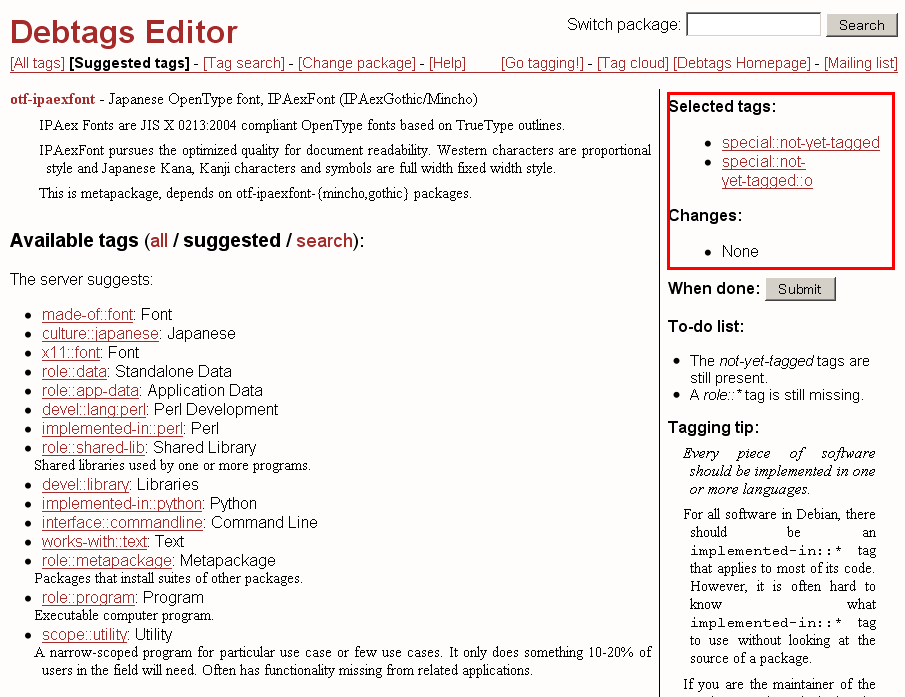
\includegraphics[height=0.5\hsize] {image201004/gotagging02.png}
 \caption{debtags タグ付け web インターフェイスの様子}
\label{fig:gotagging02}
\end{center}
\end{figure}

\begin{itemize}
 \item 選択したパッケージの説明(画面左上)
 \item 利用可能なタグの区別:all(すべて)/ suggested (おすすめ)/ search (検索)
 \item タグの一覧(画面左下)
 \item 既に付けられた・付けられるタグ(画面右)
\end{itemize}

\clearpage

\subsection{修正が必要なタグ}

まだキチンとタグ付けがされていないパッケージには、赤い×印と共に以下のような注意が表示されます。
ここからまず直していくことを考えましょう。

それぞれ以下のような意味合いです。

   \begin{table}[h]
    \begin{center}
      {
        \begin{tabular}{l|l} \hline
                表示される注意 & 意味合い \\ \hline \hline
The not-yet-tagged tags are still present. & このパッケージはまだタグ付けが終わってないよ、のタグが残ってます。 \\
An implemented-in::* tag seems to be missing. & このソフトはほげほげ言語で実装されています、ってタグ付けしようね \\
A role::* tag is still missing. & このソフトの役割をタグ付けせよ(role は必須です) \\
A devel::lang:* tag seems to be missing. & ほげほげ言語開発用のタグを付けましょう \\
           \end{tabular}
        }
     \caption{タグ付けがされていないパッケージの注意書き}
     \label{tagwarning}
    \end{center}
    \end{table}

これを踏まえて以下のような作業をします。

\begin{itemize}
 \item まだパッケージを指定していないなら、パッケージ名をクリック
 \item 提示されるタグや検索したタグをクリックして追加
 \item 必要ないタグが付けられている場合はクリックして削除
 \item 画面右側の「Selected tags:」と「Changes:」を見て、問題がないことを確認\fgref{fig:gotagging03}
 \item 最後に submit 
\end{itemize}


\begin{figure}[H]
\begin{center}
 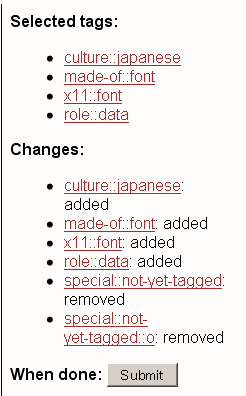
\includegraphics[height=0.5\hsize] {image201004/gotagging03.png}
 \caption{画面右側の「Selected tags:」と「Changes:」を確認!}
\label{fig:gotagging03}
\end{center}
\end{figure}


これだけで作業は終わりです。簡単ですね!


\subsection{どんなタグがあるの?}

タグ付け自体は簡単なものなので、パッケージに対して適切なタグを付けることが肝要なのですが、
すべてのタグを覚えることは大変すぎるのであきらめて、
サイトが適宜提示してくれるものの中から選択しましょう。
あと一応ガイドラインもあります (\url{http://wiki.debian.org/DebTaggingGuidelines})

で、最初に「推奨」タグが表示されています。適当なものがあればここから選ぶのもいいですが、お勧めは
\begin{itemize}
 \item 他の似たパッケージを見てみる → 同じタグ使う
 \item all を選んで、検索窓からキーワードでタグを検索する
\end{itemize}
です。


\subsection{その他疑問点}

\begin{itemize}
 \item 悪意のあるコミットについては? spammerなどは大丈夫か

        コミットされたタグについては一応ブラウザのクッキーが紐付けられていて、レビュー時に重宝している模様です。

 \item コミットは誰でもできる?レビューは?
 
        レビューするには Alioth の 'debtags' グループに参加する必要があるそうです。
        また少なくとも Debian を使っていないと、レビューの分類をする際、細かな点でうまく判断できないだろうということでした。
\end{itemize}


\subsection{最後に}
Happy tagging!

% from debianmeetingresume200912-kansai.tex
\dancersection{Debian を使って愉しむ Open Street Map 入門}{たなかとしひさ}
\index{open street map}

\subsection{Open Street Map をご存知ですか?}

\begin{figure*}[h!]
    \centering
    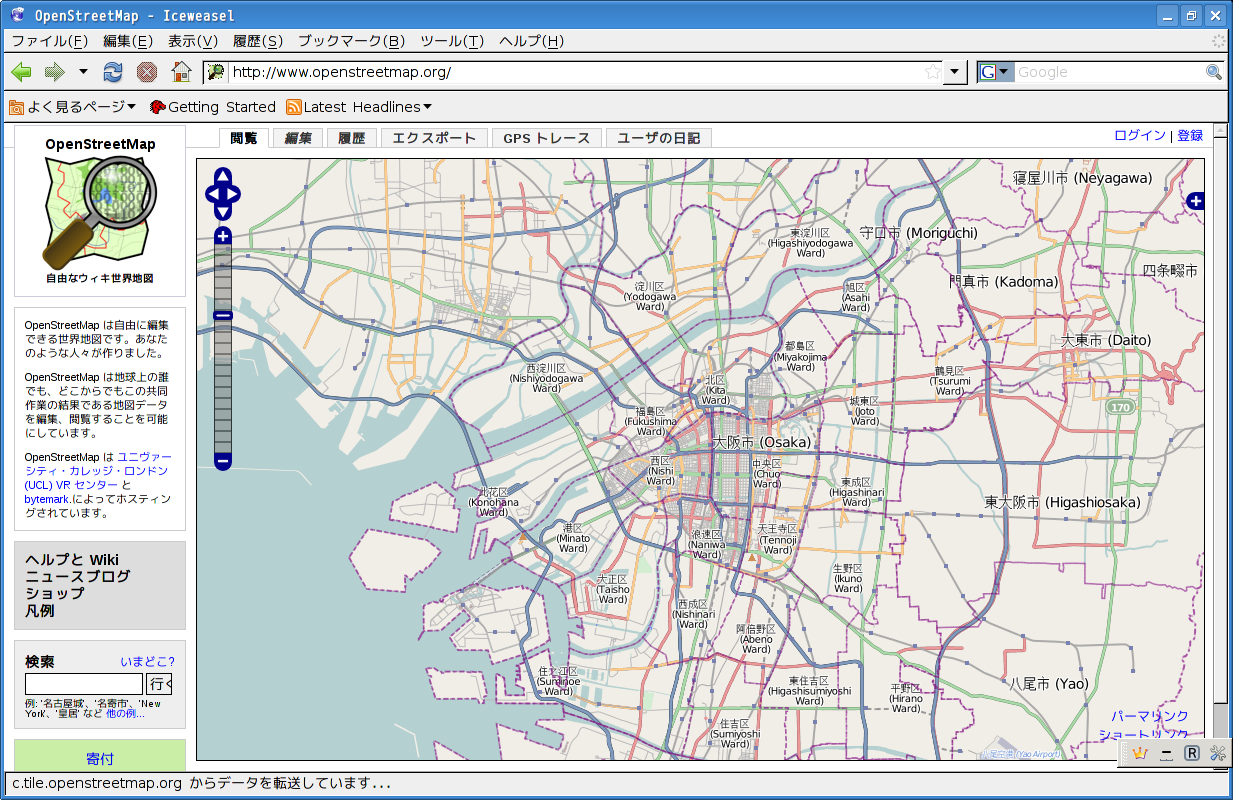
\includegraphics[scale=0.3]{image200912/debianosm1.png}
    \label{fig:debianosm1}
\end{figure*}

2009年度12月のDebian 勉強会のお知らせで、
\url{http://www.openstreetmap.org/} にアクセスして、お住まい近辺の地図を
見て頂けたらと案内しました。

ご覧になられた皆さん、感想はいかがでしょうか。

「すげぇ、素晴らしい!」

「Google Map の廉価版?」

「Debian と何の関係があるのさ?」

 等など、色々な感想があると思います。

今回の勉強会では、Debian の応用として、Debian を使って、この
OpenStreetMap(以降、OSM と表記)について、一緒に勉強していきましょう。

\subsection{免責}
\begin{itemize}
 \item このテキストは、たなかとしひさ(tosihisa@netfort.gr.jp)が書いたものです。
 \item このテキストには、間違いがあるかもしれません。
 \item 記載内容は、できるだけ最新(2009年12月)の事情にあわせて記載したつもりですが、時間の経過で内容が変化する場合があります。
\end{itemize}

\subsection{OpenStreetMap(OSM) って何ですか?}
\url{http://wiki.openstreetmap.org/wiki/Ja:Main_Page} からの引用です。

\begin{quotation}
OpenStreetMapは道路地図などの地理情報データを誰でも利用できるよう、フリー
の地理情報データを作成することを目的としたプロジェクトです。自由に使える
と思っている地図の多くが実は法的・技術的に問題があり、人々がクリエイティ
ブに、生産的に、あるいは今まで予期しなかった方法でそれを 利用する事を妨げ
ているため、このプロジェクトは開始されました。
\end{quotation}

\subsection{Debian と OSM}

今回の関西 Debian 勉強会は、従来のテーマとは異なり、異色でもあります。
「OSM って、Debian と何か関係あるの?」と言われると、確かに強い関係…
はありません。

しかし、Debian と OSM を組み合わせる事で、

\begin{center}
 \textbf{{\large「自由度の高い」地図ソフト環境} }
\end{center}

が実現できます。これは、画期的な事だと筆者は考えています。

Debian で、どれだけ素晴らしい地図ソフトが .deb になって apt で得ら
れるとしても、地図データが無ければ魅力を欠きます。

Debian を始めたとした Linux ディストリビューションは、「自由に使う
事が出来るコンピュータソフトウェア環境」を実現できるものですが、それと
OSM とを組み合わせる事で、自由に使う事が出来るコンピュータソフトウェア環
境の中に、「地図の閲覧」を含める事が出来ます。

Debian もそうであるように、OSM もまた、「一部の特権階級」のもので
はありません。望めば、誰でもが自由に使う事が出来ます。
OSM は、使うには一苦労かかる事もしばしばありますし、地図自身、日本国内で
は十分に揃っているとは言えない状況です。

しかし、誰でもが、自由に使える地図データを提供できる事は、Debian が目指す
ゴールと重なります。

また、「単に Debian を使う」だけでなく、Debian の応用事例を増やす事は、
Debian コミュニティに取っても有益と考えています。
Debian は、サーバ、医療、組込みなど、様々な分野で使われています。
その中に「自由に使える地図環境」を加える事が出来ます。

\subsection{OSM のライセンス}

OSM の地図データは、Creative Commons Attribution-ShareAlike 2.0、簡略系
で書くと CC BY-SA (表示-継承)です。
\footnote{\url{http://wiki.openstreetmap.org/wiki/Ja:OpenStreetMap_License}}

なお、OSM の地図データのライセンスは、2009年12月現在 Open Database License (ODbL) への移行が検討されています。
\footnote{\url{http://wiki.openstreetmap.org/wiki/Ja:Open_Database_License}}

12月の関西 Debian 勉強会実施頃には、もしかするとライセンスが変更されているかも知れません。

\textbf{{\large *急募*} }

日本の OSM コミュニティは、ODbL に関する情報を必要としています。
ODbL に詳しい(出来れば)日本語の情報がありましたら、筆者までお知らせ下さいますと助かります。

ODbL は、日本ではまだ認知が低いためか、日本語の情報が少なく、どの様な情報
でも構いませんので、筆者までお知らせ下さいますと助かります。

\subsection{OSM の特徴}

\subsubsection{OSM の地図データは、ビットマップではなくベクトルデータ}

OSM の地図データはベクトルデータです。
\url{http://www.openstreetmap.org/} や、\url{http://osm.jp/} から参照でき
る地図画像は、そのベクトルデータをビットマップデータへレンダリングしたも
のです。

地図データがベクトルデータなので、地図の表現能力自身は、ビットマップに比
べると劣りますが、ベクトルデータの場合、拡大・縮小が自由に行える事と、ルー
ト探索が可能になります。

OpenStreetMap の地図データを用いたルート探索サービスを提供しているサイト
の一つに、CloudMade があります。
CloudMade の地図サイト (\url{http://maps.cloudmade.com/}) にアクセスして、
大阪(梅田)から、関西 Debian 勉強会までのルート探索結果を\fgref{fig:debianosm2}に示します。

\begin{figure}[h]
 \centering
 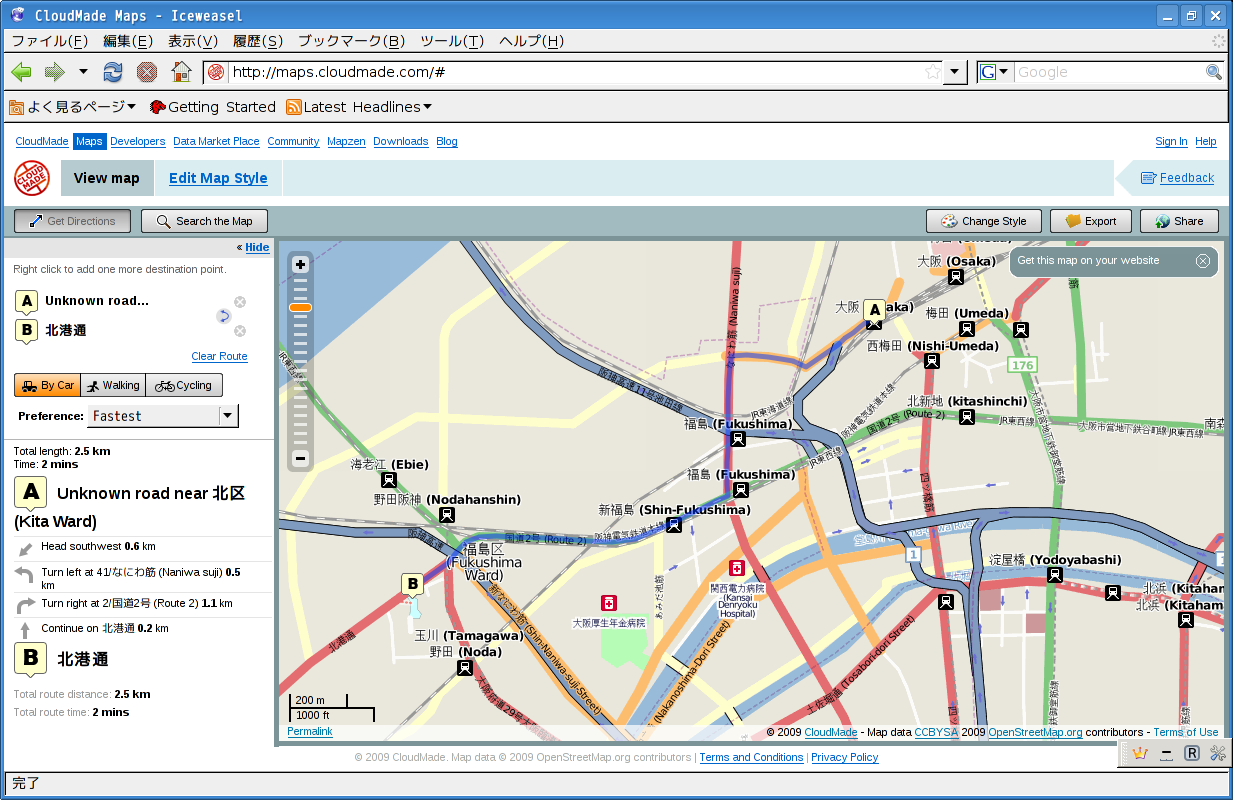
\includegraphics[scale=0.4]{image200912/debianosm2.png}
 \caption{CloudMade による関西 Debian 勉強会へのルート探索図}
 \label{fig:debianosm2}
\end{figure}

OSM の地図データ自身がまだまだ不足している事と、地図データの精度が足りな
いので、期待したルート探索結果にはまだならないかも知れませんが、この様な
ルート探索が行える可能性を OpenStreetMap は持っています。

\subsubsection{地図データの作成は、アカウント登録さえすれば誰にでも可能}

\begin{wrapfigure}{r}{30zw}
 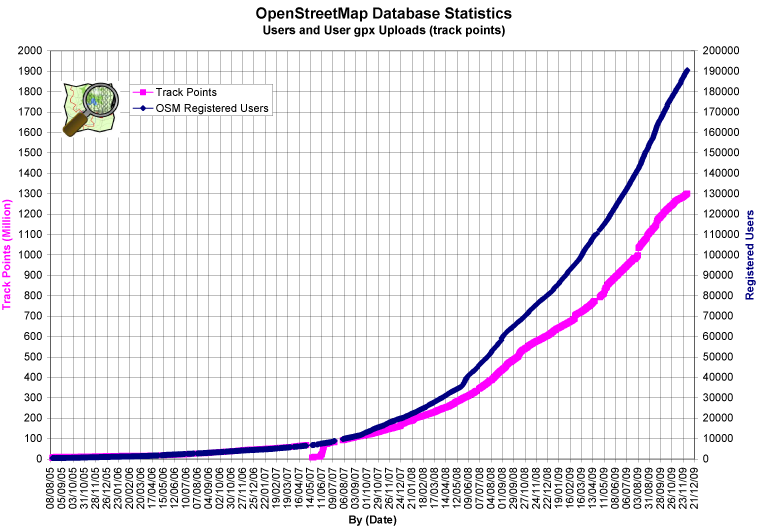
\includegraphics[scale=0.5]{image200912/debianosm3.png}
 \caption{OSM登録者数と作図データの推移グラフ}
\end{wrapfigure}

OSM の地図データの作成は、OSM へのアカウントを登録すれば誰にでも作成、編
集が可能です。

2009年5月に、OSM ユーザ数は 100,000 を越えました。右に、その登録者数と
作図データの推移グラフを示します。
(出典:\url{http://www.opengeodata.org/2009/03/17/osm-passes-100000-users/})

\clearpage

\subsubsection{Wiki の考え方をベースにしている}

地図データの作成は、Wiki の考え方が根本にあります。A さんが作図したデータ
を B さんが修正する事が可能です。
Wiki の悪い面 いわゆる「荒らし」的な事も、やろうと思えば出来てしまいます
し、地域によっては「編集合戦」があるのも事実です。

しかしながら、Wiki ベースであるので、「より良い方向に向かって修正する」事
が可能であり、例えば一方通行の方向が逆である事を見つけた場合、アカウント
を持っていれば修正する事が出来ます。

\subsubsection{地図データはオフラインでも利用できる}

GoogleMap は実に便利ですが、基本はオンライン、要するにインターネットに繋
がっている環境下である事が前提にあります。
また、GoogleMap が提供する地図は、事前に Google の書面に同意を得る事無し
に独自の技術によるアクセスや地図の複製は出来ません。

出典:
\begin{itemize}
 \item \url{http://www.google.co.jp/intl/ja_jp/help/terms_maps.html}
 \item \url{http://www.google.com/intl/ja_ALL/help/terms_local.html}
\end{itemize}

これは、オフライン対応地図閲覧ソフトは、Google Map の地図データを書面によ
る同意無しに使えない事を意味します。
オフラインでも地図を閲覧できるソフトに Mobile GMaps
(\url{http://www.mgmaps.com/}) があります。これはオンラインでもオフラインでも使
用できる PDA や SmartPhone 向け地図ソフトですが、上記の理由から、このソフ
トは Google Map の地図に対応していません。

誤解の無い様に付け加えると、筆者は GoogleMap のあり方は問題視していません。
GoogleMap が提供するサービスは、これらを補うに十分と考えています。

大事な事は、インターネットがどこでも安価に使える様になったとは言え、それ
は「全世界から見ればごく一部」でしか無いと言う事です。
日本でも、山間の地域に行くと、携帯も圏外になる場合があります。

この様な場合でも、地図データをオフラインで持っておけば、圏外でも地図を閲
覧できますし、圏内でもパケット課金を気にする必要はありません。

OSM の地図データをオフラインで見られるソフトの一つに、navit
(\url{http://wiki.navit-project.org/index.php/OpenStreetMaps}) があります。
navit は後の章で紹介します。

\subsection{(今だけの愉しみですが)走行ログになります}

筆者はバイクに乗り、アチコチに移動するのが趣味で、GPS を持って出かけてロ
グを取って後で眺めたりします。その時、「単にログを見る」だけではなく、
「そのログを元に地図を作図する」事が出来れば、さらにより良いと考えていま
す。

筆者が OSM に地図データをコミットし始めた頃は、大阪は殆ど何もありませんで
した。記憶ですが、名神か阪神高速の一部があった程度です。どなたか、大阪を
通過された方が作図されたのだと思います。

筆者はまず、大阪のシンボル御堂筋を作図しました。続けて、四ツ橋筋を作図し
ました。当時は「広大な白地図」でしたので、どこを走っても作図できましたが、
最近の大阪の OSM 地図の発展は目覚しく、少し考えてログを取らないと、誰かが
既に作図済みの所を走っているだけになります。

近畿地方で最も OSM の作図が進んでいるのは、滋賀県長浜市の OSM 地図と考え
ています。
滋賀県長浜市の OSM 地図発展は目覚しいもので、「よくぞここまで作図したもの
だなぁ・・・」と感嘆する事しきりです。

筆者は、「自由に使える地図を【使いたい】」と言う理由で OSM に注目し始めま
した。が、ミイラ取りがミイラと言う訳ではありませんが、目的が「自由に使え
る地図を【作ること】」に変ってきているのも事実です。

\subsection{OSM へのコミットは、地域社会への貢献にもなりえます。}

筆者は常々、事 OpenSource の成果は、地元社会にもつながればと考えています。

プログラミング言語 Ruby は、島根県の IT ならびに OpenSource 促進に良い影
響を与えたと考えています。OSM は、それと同じ効果を持ちえると考えています。

「地図」と言うのは、OpenSource コミュニティに限らず、誰にでも一応の興味が
あります。私の母はコンピュータ環境と無縁な生活を送りつづけていますが、母
は山歩きが趣味なので地図帳は持っています。

また、日本は地震が多いので、避難場所への地図を載せた看板を目にすると思い
ます。
筆者は、OSM が地震等の災害発生時に役に立つ日が来ればと考えています。
地震等の災害で、道路が分断された場合、どこからどこまでが通行不可なのかど
うかを、迅速に反映できる仕組みを、OSM は持っていると考えます。

また、視力が弱く、地図を見る事が出来ない場合にも、OSM の地図をベースに
「触地図」を作ってみたケースがあります。

現在の OSM の地図データは、日本国内で見れば、まだまだ足りないのが現状です
が、「地図」は殆どの人には、少なからず関係があるものですので、

この様に、様々な形での応用を OSM は持っています。

\subsection{OSMへの参加}

OSMへの参加は、
\url{http://wiki.openstreetmap.org/wiki/Ja:Beginners_Guide}を参考にすると
良いでしょう。基本的には下記の事をしていきます。

\subsubsection{OSMアカウントの作成(初めの1回だけ)}

\url{http://www.openstreetmap.org/create-account.html}にアクセスして、
OSMアカウントを作成します。同時に、
\url{http://wiki.openstreetmap.org/index.php?title=Special:UserLogin&type=signup&uselang=ja}
にアクセスして、OSM の Wiki アカウントを作成しておくと良いでしょう。

OSMは、地図データのアップロードは「OSMアカウント」を用いますが、それ以外
にも OSM の Wiki ページ(\url{http://wiki.openstreetmap.org/})がありますの
で、OSMに関する情報公開に用いると良いでしょう。

アカウントの作成は初めの1回だけですが、後々のGPSログのアップロードや作図ではOSMアカウント情報が必要です。

OSM作図の流れを\fgref{fig:debianosm4}に示します。

\begin{figure}[h]
 \centering
 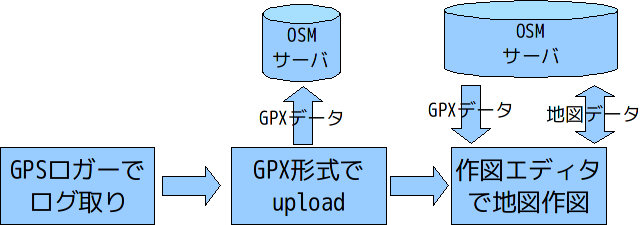
\includegraphics[scale=0.7]{image200912/debianosm4.png}
 \caption{OSM作図の流れ}
 \label{fig:debianosm4}
\end{figure}


\subsubsection{GPSロガーでログ取り}

GPSロガーを持って、まだ地図データの無い白地図の所に行き、GPS データをログ
していきます。

「マッピングパーティ」と言う催しがあります。これは、OSM同好の集まりでGPS
等を持ってログを取る催しです。この「マッピングパーティー」に参加するのも
良いでしょう。

\subsubsection{GPSログデータをアップロードする}

GPSロガーのデータをGPX形式にして、OSMサーバにアップロードします。

技術的には、GPSログデータをアップロードしなくても作図そのものは可能ですが、「GPSを元にした道である事」への根拠として、GPSログデータはアップロードしておいた方が良いでしょう。

\subsubsection{地図データを作成、編集する}

\begin{figure}[h]
 \centering
 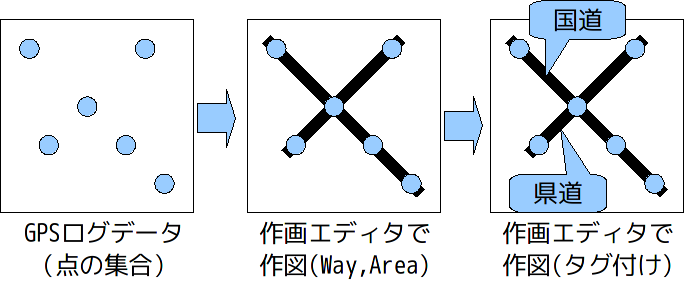
\includegraphics[scale=0.7]{image200912/debianosm5.png}
 \caption{作図イメージ}
 \label{fig:debianosm5}
\end{figure}

GPSログデータを元に、OSM作画エディタを使って、実際に作図していきます。

GPSログデータは、点データの集合ですので、それをOSM作図エディタで繋いで行き、線にしていきます。

次に、その線データが国道なのか、県道なのか、一方通行かどうかの情報を付加していきます。これを、「タグ付け」と言います。
作図のイメージを\fgref{fig:debianosm5}に示します。

\subsubsection{マップを描画する! }
出来上がった地図を見てみましょう!
地図のレンダリングには少し時間がかかりますが、早ければ1時間位でレンダリングされます。

\subsection{OSM へ参加するには、GPSロガーは不可欠なの?}

GPSロガーが無いからと言って、OSMに参加できない事はありません。GPSロガーが無くても、下記の形でOSMへコミットできます。

\begin{itemize}
 \item 使ってみる。\\
OSMは地図データですので、実際にそれが現実とあっているかが重要です。とにもかくにも、OSMを使ってみて下さい。Debian と同様に、「それを使う」だけでも、貢献として充分なのです。
 \item 間違いを修正する。\\
OSMの作図は、できるだけ正しくなるように作図が進んでいますが、例えば一方通行の方向が逆だったり、国道/県道の番号が間違っている場合もあります。
この様な場合、作画エディタでOSMデータをダウンロードできますので、間違いのある部分をダウンロードして修正してアップロードすれば、間違いが修正できます。
\end{itemize}

\subsection{Debianで使える OSM (GIS) 関連ソフト}
 Debian は、メンテナの尽力により豊富なバイナリパッケージを使う事ができますが、
 OSM 関連で利用できるソフトウェアを下記に示します。もちろん、これだけではありません。
 私見ですが、GPS を扱うソフトは、Windows よりも Debianの方が多岐に渡っていると感じています。

\subsubsection{gpsd}

\begin{commandline}
# apt-get install gpsd
\end{commandline}

gpsd は、OSMでは必須では無いのですが、Debian や Linux でGPSデータを受信する際にほぼ標準として使われているので紹介します。
このソフトは、GPS 受信機と PC を接続し、NMEA-0183 センテンスまたは GPS の独自プロトコルと通信し、現在の緯度経度、UTC 時間を処理します。

Debian で動作する地図関連のソフトは、GPS 受信機と直接通信せず、gpsd を経由して緯度経度の情報を得るものが多いです。
gpsd を経由させる事で、GPS 受信機一つに対し、複数の(GPS を必要とする)ソ
フトが使えるようになります(\fgref{fig:debianosm6})。

\begin{figure}[h]
 \centering
 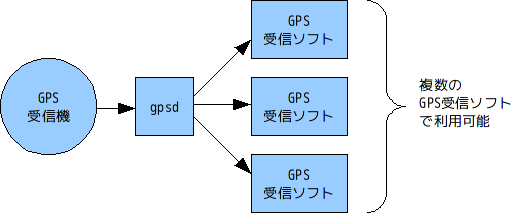
\includegraphics[scale=0.9]{image200912/debianosm6.png}
 \caption{gpsdの動作イメージ}
 \label{fig:debianosm6}
\end{figure}

また、gpsd は、NTP サーバ向けの時刻源としても機能します。NTP(ntpd) とは、共有メモリドライバを介して行います。ただし、gpsd を NTP サーバ向けの時刻源にしても、NTP 階層の Stratum 1 の精度になるわけではありません。これは、gpsd が時刻情報を受信する時、共有メモリに書き込むときに「ゆらぎ」が生じるからです。

Debianと OSM からは少し外れますが、もし、GPS を時刻源として Stratum 1 相当の NTP サーバを作るならば、"1PPS (one pulse per second)" 出力つき GPS が必要になります。

1PPS とは、「正確に1秒のパルス」を発生するもので、このパルスを Linux カーネルで捕まえる事で、時刻のゆらぎを少なくします。

\subsubsection{gpsbabel}

\begin{commandline}
# apt-get install gpsbabel
\end{commandline}

gpsbabel は、様々な GPS データの形式を変換するソフトです。

GPS データの「基本的な仕様」としては、NMEA-0183 センテンスがその基本なの
ですが、GPS 受信機ベンダーは、独自フォーマットでデータを保存する場合があ
ります。それは様々なGPSベンダーから、様々なデータ形式があります。Google
Earth の “.kml”形式も、そのGPSログの保存形式の一つです。

gpsbabel は、その GPS データ形式を変換するソフトです。

OSMが採用しているGPSログ形式は、<time>タグ付きGPX形式のみですので、もし
GPS受信機、あるいは付属ソフトが<time>タグ付きGPX形式に対応していない場合、
gpsbabelで変換しなければならない場合があります。

参考に、NMEA-0183 センテンスのGPSログデータを GPX に変換するには、下記の
様に実行します。

\begin{commandline}
$ gpsbabel -w -r -t -i nmea -f {nmea-log-file} -o gpx -F {GPX_DATA}.gpx
\end{commandline}

\clearpage

\subsubsection{Merkaartor (発音は"メルカトル"です)}

「deb \url{http://www.backports.org/debian} lenny-backports main contrib non-free」を、/etc/apt/sources.listに追加します。

\begin{commandline}
# apt-get update
# apt-get -t lenny-backports install merkaartor
\end{commandline}

\begin{wrapfigure}{l}{25.5zw}
 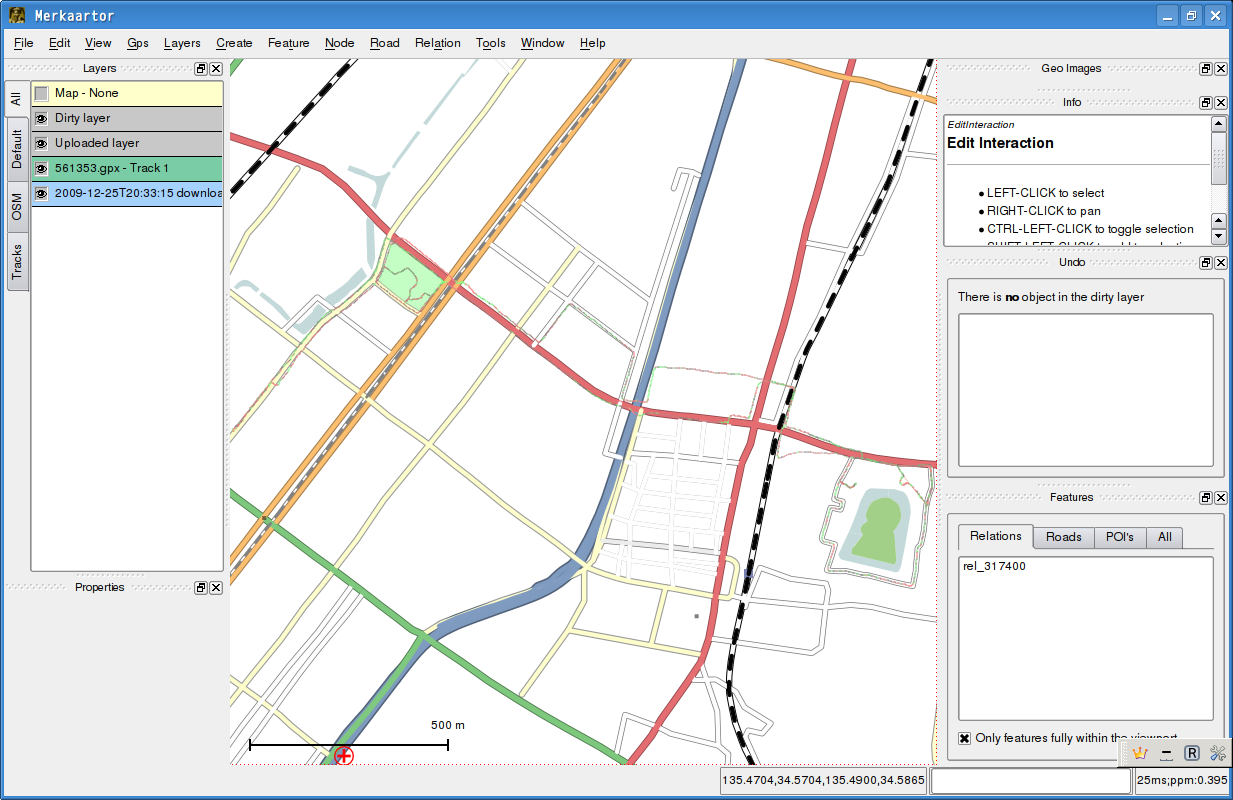
\includegraphics[scale=0.28]{image200912/debianosm7.png}
 \caption{Merkaartorイメージ}
 \label{fig:debianosm7}
\end{wrapfigure}

 Merkaartor(\fgref{fig:debianosm7} は、OSM の作図ソフトです。
 OSM 向けの作図ソフトは、大きく3つあります。

\begin{enumerate}
 \item Potlatch \\
Potlatch は、フラッシュベースの作図ソフトで、Web ブラウザがあれば使う事が
出来ます。
 \item JOSM \\
JOSM は、Java で書かれた作図ソフトで多機能です。Java 版なので、Debian で
も Windows でも動きます。
 \item Merkaartor
Merkaartor は、Qt ライブラリを使って書かれた作図ソフトです。
JOSM と同じく Debian でも Windows でも動きます。
\end{enumerate}

どれがお奨めか、これは3つとも自由に使えるソフトですので、3つ試して一番
自分に合うものを選んで下さい。一概にどれが良い・悪いと言うのはありません。
ただ、私見ですが、Merkaartor は多機能で無い分、初心者にとってはかえって分
かりやすいと考えています。

Debian lenny に入っている Merkaartor は少しバージョンが古く、Debian
Backportsサイト(\url{http://www.backports.org/}) から、出来るだけ新しい
Merkaartor をインストールすると良いでしょう。

\subsubsection{navit}

「deb \url{http://navit.latouche.info/debian} lenny main」を、/etc/apt/sources.listに追加します。

\begin{commandline}
# gpg --recv-keys CB229096
# gpg --export -a CB229096 | apt-key add -
# apt-get update
# apt-get install navit
\end{commandline}

\begin{wrapfigure}{r}{23zw}
 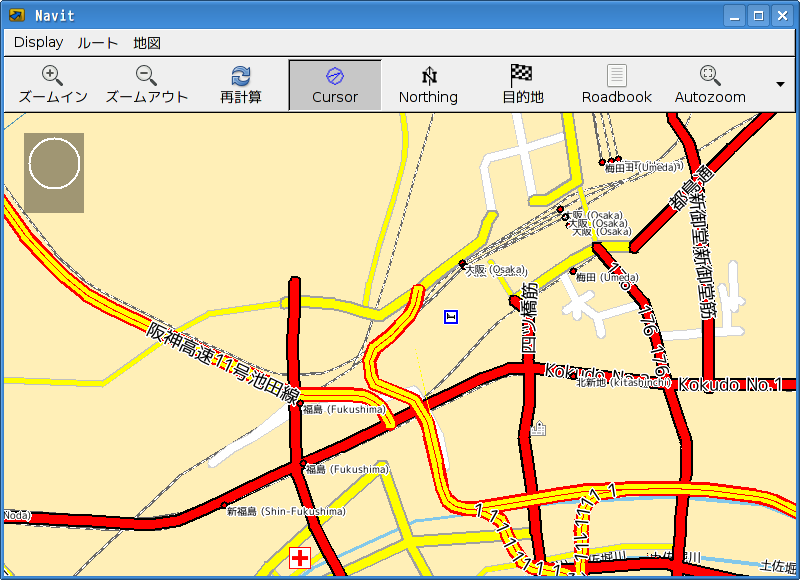
\includegraphics[scale=0.38]{image200912/debianosm8.png}
 \caption{navitイメージ}
 \label{fig:debianosm8}
\end{wrapfigure}

navit(\fgref{fig:debianosm8}) は、OSM 地図データに対応した地図表示ソフトです。gpsd が必要で、
gpsd から現在の緯度経度を取得し、OSM 地図データと重ね合わせ表示する事が出
来ます。
navit は OSM 地図データを事前に取り込む方法ですので、ネットが使えないオフ
ライン環境下でも地図を見る事が出来ます。

筆者は Debian Lenny をインストールした EeePC に、gpsd と navit をインストー
ルし、大阪から新潟まで使ってみたことがあります。
実際の走行は、殆どが高速道路ですので、ナビと言うほどのものはありませんで
したが、私が念願としていた、「自由な OS で、自由なソフトで、自由な地図デー
タでナビをする」と言う事が達成できた瞬間でした。

筆者はまだまだ、Debian は初心者の域を出ません。もし Debian にあるパッケージで、良いものがありましたら紹介下さい。

\subsection{筆者の GPS ログ機器}

筆者は、主に2台の GPS 受信機を使ってログを取っています。

\subsubsection{GT-31}

GT-31 は、小型防水の GPS ロガーで、バイクに取り付けることが出来ます。

GT-31 の良い所は、GPS ログを SD カードに保存する事が出来るので、記録容量
が SD カードの容量次第で大きく出来る点です。また、IPX7相当の防水性能があ
ります。IPX7 相当の防水機能とは、1m の水中に、30分間沈んでいても内部に水
が入らない構造を指します。

筆者は GT-31 の SDカードに、NMEA-0183 の形式で保存しています。

\subsubsection{HI-406BT}

GT-31 と併用して、HI-406BT も使っています。

HI-406BT は、純粋な GPS 受信機であり、この機器自身にログ機能はありません。
HI-406BT は Bluetooth インターフェースなので、筆者は Bluetooth 付きの
PDA や PC に、これも NMEA-0183 の形式で保存するようにしています。

\subsubsection{HOLUX m-241}
HOLUX m-241 は、単3乾電池一つで動作する小型 GPS ロガーです。

小型でありながら、ロガーとしての記録容量が大きく、130,000点のログが可能で
す。加えて Bluetooth に対応しています。筆者が OSM に作図し始めた頃は、こ
の m-241 でログを取っていました。
残念な事に、筆者の m-241 は壊れてしまい、今は GT-31 と HI-406BT を併用し
ています。

GPS は、余裕があれば2台欲しいです。白地図を作図するときは、やはりGPSログ
から作図しますので、ログ取り忘れはかなり寂しい事になります。

GT-31 は、GPS ログしない。と言う選択肢が無く、常にログします。m-241 は、
ボタンのトグルでログする・しないを選択できますが、ついうっかり忘れてしま
う事がありますので、GPS ログを取る・取らないが選択できる GPS 受信機を使う
場合、GPS ログ状態がすぐに確認できるものを選ぶと良いでしょう。

\subsection{GPSロガー選び方ノウハウ}

\subsubsection{DOP (Dilution of Precision - 精度低下率) が分かるものを選ぼう}

GPS レシーバは、「GPS 衛星から現在位置をもらう」のではなく、GPS 衛星から
正確な時刻と GPS 衛星の移動情報を元に、「GPS レシーバが自力で現在地を計算
する」仕組みです。

そのため、計算結果から、精度がどれくらい低下しているかを判断する事が出来ます。
これは GPS 衛星一つから現在地を知るのではなく、最低3つの GPS 衛星から現
在地を計算するためです。

DOP は、小さければ小さいほど精度が良い事を示します。この DOP は、受信した
(計算に選択した)GPS 衛星のばらけ具合によります。DOP には、水平方向の
HDOP、垂直方向の VDOP 、位置を示す PDOP があります。

下記のページに記載がありますが、OSM は、PDOP の値は 4 より下、2 より下な
らかなり良く固定されているとあります。

\url{http://wiki.openstreetmap.org/wiki/Ja:Recording_GPS_tracks}

筆者自身、作図のために GPS ログを取る時は、DOP 値には相当気を使っています。

GPS ロガー "GT-31" は、DOP 値を表示することが出来ますので、筆者が GPS ロ
グを取る時は、現在の緯度経度よりも、DOP 値を表示させるようにしています。
DOP をログする GPS ロガーを使用した場合、GPX ログにも DOP を残す事が出来
ますので、JOSM や Merkaartor でも視覚的に確認できます。

NMEA-0183 センテンスの場合、GSA センテンスがこれにあたります。

\subsubsection{外部アンテナが付けられるのと付けられないのでは大違い}

GPS 受信機には、外部アンテナを取り付ける事が出来るものがあります。
筆者は "HI-406BT" と言う Bluetooth GPS レシーバも使うのですが、これには外
部アンテナを取り付けることが出来ます。

外部アンテナを取り付けることで、GPS 信号の感度が上がり、精度が向上します。
また、外部アンテナは概ね防水型ですので、外部アンテナを車の屋根に取り付け、
天候に左右されずにログを取る事が出来ます。

\subsubsection{測位精度の誤差}

最近の GPS 受信機は精度が向上し、概ね「10m 2drms」の範囲です。
「2drms」と言うのは、これを半径とする円内に、およそ 95\% の測位点が入る事
を表します。
10m 2drms ならば、半径10m の円内に 95\% の測位点が入る事を示します。

半径10m だと、地図として使うのに誤差としては大きいかも知れませんが、DGPS
だと 5m 2drms にまで誤差が少なくなるものもあります。
GPS 受信機を購入する時は、この 2drms の値は確認しておくと良いでしょう。

\subsubsection{バッテリーの持ちと形状}

1時間程度のログであればあまり問題はありませんが、バイクツーリング等でほ
ぼ1日乗りっぱなしで GPS ログを取る場合、GPS 受信機のバッテリーも気になり
ます。

GPS 受信機のバッテリーの持ちもそうですが、バッテリーの形式、例えば乾電池
か専用電池かも、利用形態に応じて考える必要があります。

最近の個人用 GPS 受信機は、USB で充電できるものがあります。これと携帯の充
電器にあるような、乾電池の電力を USB に変換して出す充電器を併用する事で、
専用電池でもバッテリーを気にせずに使う事が出来ます。

せっかくの GPS 受信機も、バッテリーが干上がると、mapper にしてみるととて
も寂しい事になりますので、バッテリーの持ちや、形状は確認しておくと良いで
しょう。

\subsection{おわりに}
OpenStreetMapは、日本ではまだまだ認知の低いプロジェクトですが、Debian
System とも十分親和性の高いプロジェクトですので、興味を持って頂けたならう
れしいです。

% from debianmeetingresume200912-kansai.tex
\dancersection{ハンドメイドGPSロガーの構築}{まさ}
\index{gps logger}

\subsection{はじめに}

これまでDebianのインストール、環境整備、ウェブアプリケーションのシステム
構築をするなどシステムを触ることはある程度経験したものの、お小遣い帳サー
バや、GPSロガーなど、何らかの実用になるものはなかなかつくれませんでした。

そこでプログラムのスキルを得るための教材として、GPSロガーを作成したので、
報告します。

これからDebianを目指す人の興味を惹き、手がかりとなって少しでもお役に立て
れば幸いです。

\subsection{GPSとは}
``Global Positioning System'' は数十個の衛星からの電波を受信して現在位置を割り出すシステムです。

原理等はいろんな書籍やインターネットに掲載されているようですので、ここでは説明を割愛します。

\subsection{GPSロガーのハード構成}
必要なハード構成は以下の通りです。

今回実際に使用したハードの概略仕様はAppendixを参照してください。
\begin{center}
        \framebox[6.5zw]{ネットブック}
        \hspace{1em}$\Longleftarrow$\hspace{1em}
        \framebox[7.5zw]{PS2-USB変換}
        \hspace{1em}$\Longleftarrow$\hspace{1em}
        \framebox[7.5zw]{GPSレシーバ}        
\end{center}

\begin{enumerate}
 \item GPSレシーバ \\
            GPSアンテナ、受信回路、信号送出回路から成り、 PS2コネクタからシリアルにキャラクタ文字でGPS情報が送出されます。
 \item PS2-USB変換 \\
            GPSレシーバから信号送出用のシリアルインタフェースをUSBインタフェースに変換するためのものです。変換ケーブルになっています。
 \item ネットブック \\
            USBインタフェースで受信したGPS情報を受け取り、ファイルに溜め込みます。また、GPS情報をいろいろ加工して楽しめます。
\end{enumerate}

\subsection{ネットブックセットアップ概要}
ネットブック購入直後からGPSロガーを構築する場合について概要を説明します。

\begin{enumerate}
      \item Debian Base systemのインストール \\
    Debian-netinst-isoを使ってBase systemをインストールします。
      \item X Window Systemのインストール
      \item Gnomeのインストール
      \item 日本語入力システムのインストール \\
    プログラム作成時必要です。今回は、``uim-anthy'' をインストールしました。
      \item NTPのインストール \\
    システム時刻自動調整用のプログラムです。
    今回はGPSを扱うため、特にシステム時刻が大切になると思われます。
      \item プログラム言語のインストール \\
    GPSロガーアプリケーション作成に必要です。
    今回は、とっつきやすく、GUIができ、
    ライブラリが豊富と言われる ``Python'' (バイトンor パイソン?)
    を選択しました。
    私にとって、確かにとっつきやすいですが、それなりに苦労しました。
    pythonのせいではなく、プログラミングというもの自体、
    思ったものがそう簡単にできるわけではないということだと思われます。
      \item Python libraryのインストール
    \begin{enumerate}
          \item PySerial \\
        シリアルポート入出力用のプログラムです。
          \item Python Tkinter \\
        GUIプログラミング用のひとつです。
          \item datetime \\
        時刻を扱うとき使います。
          \item os, os.path \\
        ファイルの開閉、読み書きするとき使います。
          \item sys(場合によって使用) \\
        コマンドパラメータを取得するとき使います。
    \end{enumerate}
\end{enumerate}

\subsection{GPSデータ出力形式}
今回使用したGPSレシーバはNMEA0183というプロトコルです。
NMEA0183では以下のような形式などでデータが出力されますが、

\begin{description}
 \item[GLL] Geographic Position, Latitude and Longitude
 \item[GSA] GNSS DOP and Active Satellites
 \item[RMC] Recommended Minimum Specific GNSS Data
\end{description}

今回は

\begin{description}
 \item[GGA] Global Positioning System Fix Data
\end{description}

という形式のみ利用しました。
\clearpage
GGA形式の仕様は次の通りです。

\begin{commandline}
GGA,123519.00,4807.038247,N,01131.324523,E,1,08,0.9,545.42,M,46.93,M,5.0,1012*42
123519.00 	= 測位時刻(UTC) 12:35:19.00
4807.038247,N 	= 緯度 48度07.038247分(北緯)
01131.324523,E 	= 経度 11度31.324523分(東経)
1 	= GPSのクオリティ; 0 = 受信不能、1 = 単独測位、2 = DGPS
08 	= 受信衛星数
0.9 	= HDOP
545.42, M 	= 平均海水面からのアンテナ高度(m)
46.93, M 	= WGS-84楕円体から平均海水面の高度差(m)
5.0 	= DGPSデータのエイジ(秒)
1012 	= DGPS基準局のID
*42 	= チェックサム
\end{commandline}

ここから、時刻、緯度、経度などのデータを利用しました。

\subsection{アプリケーション作成}
いよいよアプリケーションの作成です。
上のGPS GGAデータを加工して、表示したり、ログをとります。


\subsection{実行}
アプリケーションを走らせます。

\subsection{今後の抱負}
今回のアプリケーションを基にいろんな展開が考えられます。
Sunday programmerとして今後も少しづつであっても、根気よく前進します。
\begin{enumerate}
      \item Open Street Mapへの貢献 
      \item Open Street Mapの利用
\end{enumerate}
地図上への現在位置の表示や、ログデータからトレース表示したりと地図情報は重要です。
この場合、種々の縮尺の地図が必要ですが、Open Street Mapはベクトルデータであることからこの点が有利です。
また、ナビのように指定した位置の地図を得る場合、これが可能なインタフェースがOSMにあれば(あるのかも知れませんが)、より柔軟に利用できるのではないかと期待しています。

\subsection*{Appendix}
% \subsubsection*{仕様}
[A] ネットブック仕様概略
\begin{commandline}
PC:       Asus EeePC 901 
CPU:      Intel Atom (1.6GHz) 
Memory:   1GB 
HDD(SSD): 4GB + 8GB 
Monitor:  8.9型、1024 x 600 
I/F:      USB 2.0 
\end{commandline}
[B] ネットブックシステム仕様 
\begin{commandline}
OS:      Debian Lenny 
Kernel:  2.6.26-2-686 
言語:    Python 2.5.2 
Library: pySerial, tkinter等 
\end{commandline}
\clearpage
[C] GPSレシーバ仕様 
\begin{commandline}
型式:       GPS-S103(Wonde proud社製)
位置 精度:  5 - 25m CEP without SA
時刻精度:   1μs synchronized to GPS time 
プロトコル: NMEA0183
動作温度:   -40 °C ~ +85 °C 
動作湿度:   5% to 90% (結露なき事) 
電源:       DC 3.7 ~ 6V, typical 5V(今回はUSBより供給)
I/F:        TTL serial(PS2コネクタ). USB option 
\end{commandline}
[D] GPSロガー実行例
\begin{enumerate}
\item ログファイル
\begin{commandline}
$GPVTG,113.96,T,,,0.00,N,0.00,K,A*7C 
$GPGGA,054832.084,3450.2455,N,13615.2118,E,1,09,01.0,253.6,M,37.3,M,,*6B 
$GPRMC,054832.084,A,3450.2455,N,13615.2118,E,0.00,113.96,260909,,,A*6C 
$GPVTG,113.96,T,,,0.00,N,0.00,K,A*7C 
$GPGGA,054833.083,3450.2455,N,13615.2118,E,1,08,01.1,253.5,M,37.3,M,,*6E 
$GPRMC,054833.083,A,3450.2455,N,13615.2118,E,0.00,113.96,260909,,,A*6A 
$GPVTG,113.96,T,,,0.00,N,0.00,K,A*7C 
$GPGGA,054834.083,3450.2455,N,13615.2118,E,1,09,01.0,253.4,M,37.3,M,,*68 
$GPGSA,A,3,03,06,07,08,11,16,19,22,25,,,,2.2,1.0,1.9*39 
$GPGSV,3,1,09,3,44,055,37,6,33,060,33,7,50,266,39,8,28,311,37*7A
\end{commandline}
\item 現在位置データ表示例
\begin{figure*}[h!]
    \centering
    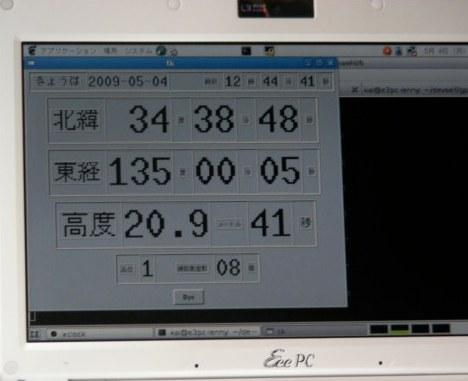
\includegraphics[scale=0.6]{image200912/handmadegpsloger1.jpg}
\end{figure*}
\item 現在位置地図表示例
\begin{figure*}[h!]
    \centering
    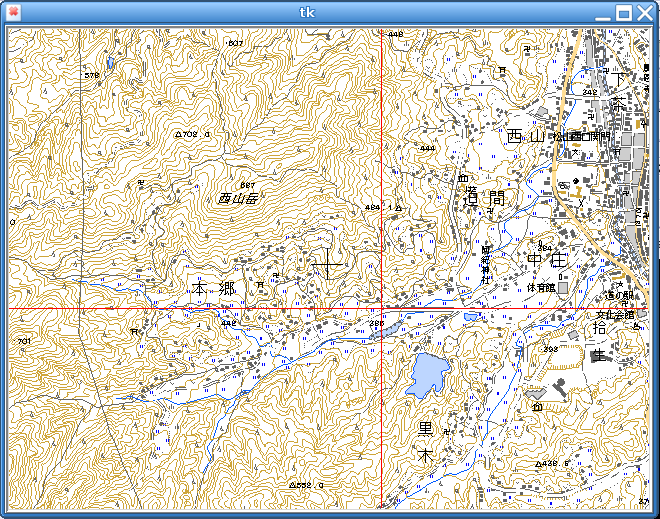
\includegraphics[scale=0.6]{image200912/handmadegpsloger2.png}
\end{figure*}
\clearpage
\item プログラム例1:データのログ
\begin{commandline}
#!	/usr/bin/python2.5
# -*- coding: utf8 -*-

#********************************************
#	
#	Created			.... 2010-01-03
#	updated			.... 2010-07-11
#	
#	object:			logging data from gps  reeiver	
#	
#	input device:	gps receiver (N103)
#	output-1:		file
#	output-2:		terminal
#	
#	data format:	NMEA-0183.
#	
# ********************************************

import	serial

# open read/write file.
d_fname = "logdata01"
fw = open(d_fname, 'w')
fw.close()
fw = open(d_fname, 'a')

# open serial line.
ser = serial.Serial('/dev/ttyUSB0', 38400, timeout = 3)
serstr = ser.portstr + "\n"
print ser.portstr

for  i in range(10):
	line = (ser.readline() ).strip() 	# get 1 line 'GPGGA' sentence.
	print line
	line += "\n"
	fw.write(line)						# write new data to log file.

fw.close()
ser.close()
\end{commandline}
%\clearpage
\item プログラム例1:データのログ
プログラム例2: 現在位置(緯度)の表示
\begin{commandline}
#!	/usr/bin/python2.5
# -*- coding: utf8 -*-

#********************************************
#	
#	Created			.... 2009-02-07 ...
#	updated			.... 2010-07-11
#	
#	object:			display latitude on the screen	
#	
#	input device:	gps receiver (N103)
#	output-1:		file
#	output-2:		screen
#	
#	data format:	NMEA-0183.
#	
#********************************************

import	serial
import Tkinter as Tk
import	string
# import os.path


root = Tk.Tk()

buff_dLa = Tk.StringVar()
buff_mLa = Tk.StringVar()
buff_sLa = Tk.StringVar()
buff_dLa.set('')
buff_mLa.set('')
buff_sLa.set('')

# define function
def cmd_quit():
	root.destroy()

# display frame

# define display font
dfont = 'Monospace '
dfont12 = dfont + '12'
dfont18 = dfont + '18'
dfont24 = dfont + '24'
dfont28 = dfont + '28'
dfont48 = dfont + '48'

# display latitude
f1 = Tk.Frame(master=None, relief= 'ridge', bd=3)
b10 = Tk.Label(f1, text="北緯", font=dfont24, relief = 'ridge')
b11 = Tk.Label(f1, textvariable = buff_dLa, font=dfont48, relief = 'ridge')
b12 = Tk.Label(f1, text="度", relief = 'ridge')
b13 = Tk.Label(f1, textvariable = buff_mLa, font=dfont48, relief = 'ridge')
b14 = Tk.Label(f1, text="分", relief = 'ridge')
b15 = Tk.Label(f1, textvariable = buff_sLa, font=dfont48, relief = 'ridge')
b16 = Tk.Label(f1, text="秒", relief = 'ridge')

for e in [b10, b11, b12, b13, b14, b15, b16 ]:
	e.pack(side='left', padx=5)

# display Exit Button
b99 = Tk.Button(master=None, text="Bye", command=cmd_quit)

# display Tate ni naraberu.
for e in [ f1, b99]:
# for e in [ f0, f1, f2, f3, f4, b99]:
	e.pack(side='top', padx=5, pady=5)

def showtime():
	# get 'GPGGA' sentence from gps receiver.
	ser = serial.Serial('/dev/ttyUSB0', 38400, timeout = 3)
	# ser = serial.Serial('/dev/ttyUSB0', 4800, timeout = 3)
	print ser.portstr
	line = ser.readline()
	words = line.split(',')
	while( not words[0] == '$GPGGA'):
		line = ser.readline()
		words = line.split(',')
	print line
	ser.close()

	# latitude
	lati = words[2]
	deg_lati = " " + lati[:2]
	min_lati = lati[2:4]
	sec_lati = str( int(float(lati[4:]) * 60 ) ).zfill(2)
	gpslati = 'latitude = ' + deg_lati + ':' + min_lati + ':' + sec_lati + ' ' + words[3] + '  '

	buff_dLa.set(deg_lati)
	buff_mLa.set(min_lati)
	buff_sLa.set(sec_lati)

	root.after(1, showtime)

showtime()
root.mainloop()
\end{commandline}
\end{enumerate}

% from debianmeetingresume201004-kansai.tex
\dancersection{ハッカーに一歩近づく Tips 〜正規表現編〜}{山下康成@京都府向日市}
\index{せいきひょうげん@正規表現}
\index{sed}
\index{grep}

\subsection{正規表現とは}

検索や置換などテキスト処理で使用する効率的なパターンマッチングの表現方法
です。
ファイル名に使う *, ? と概念は同じです。 
今回、説明するのは

\begin{commandline}
^$.[]*\(){}    
\end{commandline}
のたった11文字+数字です。

\subsection{事前課題}

/etc/passwd を解析してユーザ binのログインシェルを表示しなさい
\begin{enumerate}
\item 思考に近い解答例
\begin{commandline}
% grep '^bin:' /etc/passwd|cut -d: -f7  
\end{commandline}
\item 空気を読んで正規表現を使った解答
\begin{commandline}
% sed -n -e 's/^bin:.*:\([^:]*\)$/\1/p' /etc/passwd        
\end{commandline}
\end{enumerate}

\subsection{正規表現で使う文字}
\subsubsection{ \^ ~と \$}
\begin{description}
      \item[{\tt \^}] 行頭に一致
      \item[{\tt \$}] 行末に一致
\end{description}
行頭(\^\ ), 行末(\$ )にマッチさせる場合の例:
\begin{commandline}
% grep '^bin:' /etc/passwd
% grep '/bash$' /etc/passwd 
\end{commandline}
grep 以外でも、emacs や vi でも同じ様に使える。もちろん, perl や awk でも...
\begin{commandline}
emacs   ->  RE search: ^bin
vi      ->  /bash$
\end{commandline}

\subsubsection{{\tt .} ピリオド}

何か一文字に一致する。
文字数だけが一致すれば良いときや
何か文字があることが重要なときに使う。

\subsubsection{列挙}

列挙したどれかに一致させたいとき。
例: bin や root など b, r で始まるユーザを表示
\begin{commandline}
% grep '^[br]' /etc/passwd
\end{commandline}
ほかには
\begin{commandline}
[! " \# ]  !, ", \# に一致
[0-9]  半角数字1文字に一致
[A-Za-z]  英字に一致
\end{commandline}

\subsubsection{[\^~列挙]}

列挙したどれにも一致させたくないとき。
例: daemon や sys など b, r 以外で始まるユーザを表示 
\begin{commandline}
% grep '^[^br] /etc/passwd    
\end{commandline}
※行頭を表す \^~ と [~] 内の \^~ とは、同じ文字だが意味が違う

\subsection{*(アスタリスク)}

すぐ前の文字/正規表現0回以上に一致。
例:
\begin{commandline}
何がいくつあっても一致
  .* 
ホワイトスペースがいくつあっても一致
  [<space><tab>]* 
\end{commandline}

\subsubsection{\{n,m\}}

すぐ前の文字/正規表現n回以上m 回以下に一致。m は省略可能
\begin{commandline}
ホワイトスペースが1個以上あれば一致
[<space><tab>]\{1,\} 
数字が1文字以上5文字以下(例えばざっと short の範囲)あれば一致
[0-9]\{1,5\} 
\end{commandline}

\subsubsection{( ) と $\backslash$n (n=1..9)}

( ) で囲んだところを順に $\backslash$1 ,$\backslash$2 ... として使える。
置換に使うと置換元の一部を使える。
vi の ex モードや、emacs の replace regexp でも使える。 
例:
\begin{commandline}
# aaa bbb 等、行頭に同じ文字が3つある時に一致 
% echo 'aaa' | grep '^\(.\)\1\1'
# abab 1212 等、行頭から2文字の繰り返しに一致 
% echo 'abab' | grep '^\(.\)\(.\)\1\2'
% echo 'abcd' | sed - e 's/^\(.\)\(.\).*$/1文字目は \1、2文字目は \2 です/' 
\end{commandline}

\subsection{事前課題の空気を読んだ解答をレビュー}
\begin{commandline}
sed -n -e 's/^bin:.*:\([^:]*\)$/\1/p' /etc/passwd
\end{commandline}
これは、

 \begin{quote}
 \begin{verbatim}
{
行頭がbin: で
何か文字が0文字以上あって
: があって
: 以外が0以上あるところを1番目のバッファにいれて
行末
}
 \end{verbatim}
 \end{quote}


というパターンがあれば、1番目のバッファを表示する。

\subsection{実例}
\subsubsection{ssh アタッカーをブロックする}
/var/log/daemon.log に
\begin{commandline}
Apr 11 04:46:07 ns sshd[31776]: Invalid user oracle from 211.233.73.66
Apr 11 09:17:05 ns sshd[5607]: Did not receive identification string from 211.155.227.20
\end{commandline}
のような行があれば、その IP アドレスを /etc/hosts.deny に登録する。
\begin{commandline}          
#! /bin/sh
# Apr 11 04:46:07 ns sshd[31776]: Invalid user oracle from 211.233.73.66
# Apr 11 09:17:05 ns sshd[5607]: Did not receive identification string from 211.155.227.20

export LANG=C
HOSTSDENY=/etc/hosts.deny

sed -n -e 's/^.* sshd.*: Invalid user \(.*\) from \([0-9][0-9\.]*\)/\1 \2/p' \
       -e 's/^.* sshd.*: Did not receive identification string from \([0-9][0-9\.]*\)/\1/p' \
        /var/log/daemon.log | sort -u |
while read NAME IP; do
        # /etc/hosts.deny
        L=`grep '^ALL : '$IP'$' $HOSTSDENY`
        if [ "$L" = "" ]; then
                echo "ALL : $IP" >> $HOSTSDENY
        fi
done
\end{commandline}


\subsubsection{ロードアベレージが3以上なら、日時とps ax の結果を /tmp/highload に残す}

\begin{commandline}
# LANG=C uptime
11:57PM  up 165 days,  2:26,  1 user,  load average: 0.00, 0.06, 0.07
\end{commandline}
上記のロードアベレージの一つ目を切り出す
\begin{commandline}
#! /bin/sh 
LOAD=`LANG=C /usr/bin/uptime | sed -e 's/^.*: \([0-9]*\)\.[0-9]*,.*$/\1/'
if [ "$LOAD" -ge 3 ]
then
      echo >> /tmp/highload
      date >> /tmp/highload
      ps ax >> /tmp/highload
fi
\end{commandline}

\subsubsection{キモ}

行頭もしくは行末を起点にパターンマッチをすると良い場合が多い。
$\rightarrow$ \^\ と \$\ とを活用

スペース区切りは TAB とスペースがいくつあるかわからない。
$\rightarrow$  * や \{n,m\} を活用
\begin{commandline}
[<SP.><TAB>][<SP><TAB>]*
[<SP.><TAB>]\{1,\}
\end{commandline}

\subsection{おわりに}

正規表現をうまく使いこなせれば操作が少なくなり、
もしくはスクリプトが小さくできて効率的。 正規表現をマスタして、ハッカーに一歩近づこう!

%-------------------------------------------------------------------------------
% from debianmeetingresume201003.tex
\dancersection{ニューラルネットワークで画像認識してみた}{本庄弘典}
%-------------------------------------------------------------------------------
\index{neural network}
\index{back propagation}
\index{がぞうにんしき@画像認識}

\subsection{はじめに}

ドキュメントスキャナで本をスキャンした際、画像のサイズが大きすぎ
るため保存に適しません。この画像を2値画像とグレースケール、カラー
画像それぞれの処理を加えることでファイルサイズを縮小し、ニューラ
ルネットを用いることによりある程度自動化できないかと考えました。
今回はニューラルネットとして一般的な三層パーセプトロンを用いた画
像判別の一例を解説します。

\subsection{三層パーセプトロンとバックプロパゲーション}

\subsubsection{三層パーセプトロン}

三層パーセプトロンは入力層、中間層、出力層と別れた三層の各ニュー
ロンが重みと呼ばれる係数で結ばれたモデルとなります(\fgref{fig:neuralnet01})。

\begin{figure}[H]
\begin{center}
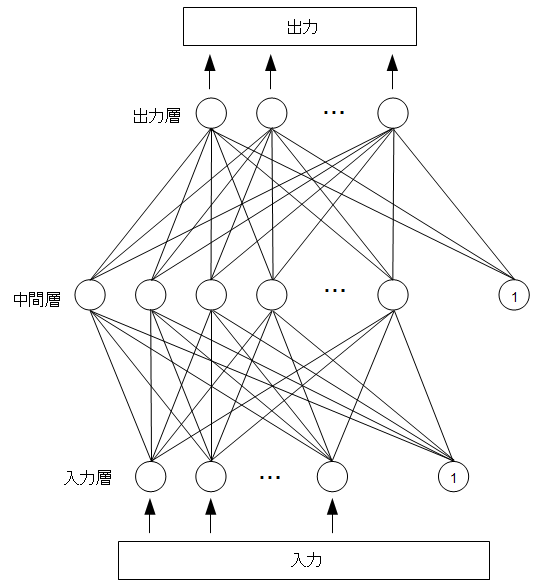
\includegraphics[width=0.45\hsize]{image201003/neuralnet01.png}
\caption{三層パーセプトロン}
\label{fig:neuralnet01}
\end{center}
\end{figure}

それぞれの重みは実数で表され、パーセプトロンが機能するためにはこ
の重みが適切に設定されている必要があります。ある入力が与えられた
際、入力値に重みを掛け合わせ、それぞれの合計に次のようなシグモイ
ド関数を適用した数値を中間層の持つ値とします。

\begin{multicols}{2}

\begin{figure}[H]
\begin{center}

\begin{equation*}
 \varsigma_1(x) = \frac{1}{1+e^{-x}}
\end{equation*}
\end{center}
\caption{シグモイド関数の式}
\end{figure}

\begin{figure}[H]
\begin{center}
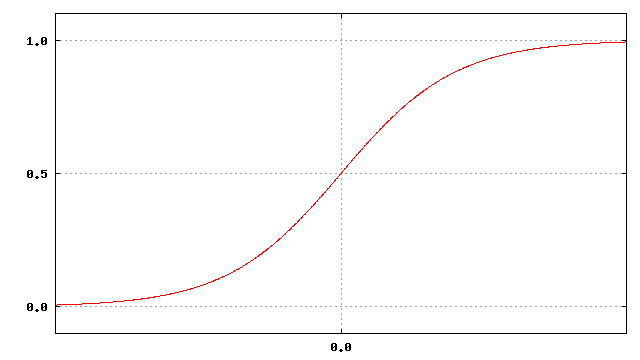
\includegraphics[width=1.0\hsize]{image201003/neuralnet03.png}
\caption{シグモイド関数のグラフ}
\end{center}
\end{figure}

\end{multicols}

各出力層も同様の計算がなされ、パーセプトロンの出力が行われます。

\subsubsection{バックプロパゲーション}

多層パーセプトロンで適切な出力を行うための学習方法として一般的な
ものにバックプロパゲーションがあります。バックプロパゲーションで
はまず入力に対する正しい出力(教師信号)を多数用意し、各重みをラン
ダムに設定します。用意された入力に対してランダムな重みからパーセ
プトロンの出力はでたらめな値となりますが、この出力と教師信号との
比較から出力層と中間層の間の重みを修正し、次いで中間層と入力層の
重みを修正することで適切な重みを探し出します。

\subsection{足し算と引き算を学習してみる}

作成したパーセプトロンとバックプロパゲーションが正常に動作するか
を確かめます。次のような入力を用意しました。

\begin{commandline}
# 学習用教師信号ペア
0.40,0.20	0.60,0.20
0.30,0.20	0.50,0.10
0.80,0.10	0.90,0.70
0.20,0.10	0.30,0.10
0.50,0.50	1.00,0.00
0.60,0.20	0.80,0.40
# 評価用入力値
*0.50,0.10
*0.50,0.40
*0.10,0.40
\end{commandline}

入力値と教師信号のペアはタブ区切りの左が入力、
右が入力に対する教師信号です。
ここでは足し算と引き算の教師信号を与えました。

\newpage

実行します。

\begin{commandline}
$ ./backprop.exe sample.txt 10000
       0 0.87640153
     100 0.26410368
     200 0.10289131
     300 0.03820243
     400 0.02475167

...(中略)...

    9600 0.00077714
    9700 0.00077174
    9800 0.00076646
    9900 0.00076128
0.4000, 0.2000  0.60, 0.18      0.60, 0.20
0.3000, 0.2000  0.50, 0.11      0.50, 0.10
0.8000, 0.1000  0.90, 0.70      0.90, 0.70
0.2000, 0.1000  0.30, 0.11      0.30, 0.10
0.5000, 0.5000  0.98, 0.02      1.00, 0.00
0.6000, 0.2000  0.80, 0.41      0.80, 0.40
0.5000, 0.1000  0.63, 0.35
0.5000, 0.4000  0.93, 0.06
0.1000, 0.4000  0.87, 0.00
Ratio=0.00075626
Count=10000
Sample=6
Input=2
Middle=4
Output=2
InputHidden0=-2.57936471,-2.20525001,-1.50656422,4.05055823,-0.66468037
InputHidden1=-1.29032439,8.71632107,-1.24344376,-0.85214732,-0.66468037
InputHidden2=2.04901840,-2.94096519,1.04866634,-1.98825291,0.29698485
HiddenOutput0=-2.91458436,-1.16992032
HiddenOutput1=5.84673832,-6.31188860
HiddenOutput2=-1.80018561,-0.42470539
HiddenOutput3=3.60356071,3.84028669
HiddenOutput4=1.40998866,-1.22885398
\end{commandline}

頼りないながらもそれなりの演算結果が出力されています。評価として
最後の数値は減算結果が負になるはずなのですが、シグモイド関数を通
すことで出力が0.0〜1.0となるため正常な結果が得られません。

\subsection{画像を分類するための入力値を考える}

画像判別の入力値として次の値を使用しました。

\begin{itemize}
\item 補正した画像のRGBの差
\item 微分した画像のRGBの差
\item 画像の複雑さ。
\item 使われている色の数
\item 平均彩度
\item FFT処理した画像の明るいピクセルを利用する
\item HSVに変換し、色素の平均を利用する
\item 色素の分散を利用する
\end{itemize}

この中から文章と絵の判別として画像のFFTを、カラー画像の判別とし
てHSVへの変換を解説します。

\subsubsection{モノクロ画像の処理・文字と絵を分類してみる}

縦書きの文章は横方向に一定の周波数を持っていると見なすことが出来
ます。これにより、文章の画像を微分しFFT処理を行った結果から振幅
を描画するとで、明るく光る点が現れることがわかりました。

\begin{figure}[H]
\begin{center}
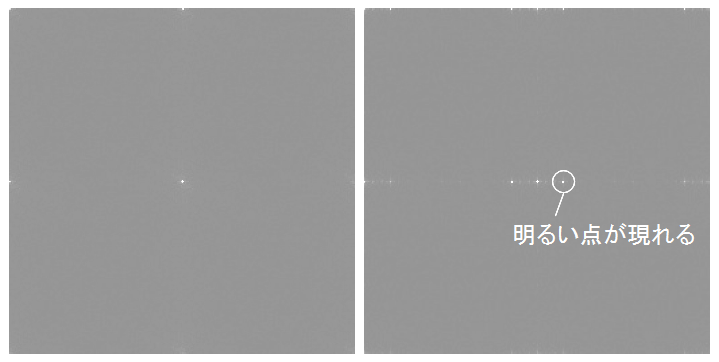
\includegraphics[width=0.9\hsize]{image201003/neuralnet04.png}
\caption{イラストと文章を微分した画像のFFT結果}
\end{center}
\end{figure}

この点の明るさを入力値とすることで、文章とイラストの判別が行える
と期待できます。

\subsubsection{カラー画像とそうでない画像を分類してみる}

カラー画像とモノクロ画像は画像のRGBをHSVに変換し、色相から判別を
行っています。

RGBのうちから最大のものをMAX、最小のものをMINとすると色相は\fgref{fig:cal-hue}の
式となります。

\begin{figure}[H]
\begin{center}
\begin{align*}
 H = & 60 \frac{G-B}{MAX-MIN} + 0, & if MAX = R\\
     & 60 \frac{B-R}{MAX-MIN} + 120,   & if MAX = G\\
     & 60 \frac{R-G}{MAX-MIN} + 240,   & if MAX = B\\
\end{align*}
\caption{色相の計算式}
\label{fig:cal-hue}
\end{center}
\end{figure}

モノクロ画像は色相を持たないため、RGBのうち青の成分を減らすこと
で黄色いフィルタをかけました。こうすることでモノクロ画像の色相の
平均は黄色となり、カラーとモノクロを判別するための入力値として期
待できます。

\subsection{学習の条件}

ニューラルネットの学習は次の条件で行いました。

\begin{itemize}
\item 入力層8個
\item 中間層24個
\item 出力層2個
\item サンプルとして使用した本23冊(漫画2冊/文庫20冊/技術書1冊)
\item ページ数6742ページ
\item 学習回数50万回
\end{itemize}

実際にこの条件で学習を行った際、
Core i7 950で7時間弱の学習時間となりました。

\subsection{判別の精度}

作成されたツールで実際に判別を行い、その精度を調べました。評価に
使用した本は学習に使われていないものを選びました。

\begin{description}
 \item[サンプル1. ライトノベル最新巻] \mbox{}\\
    240ページ中、人間の判別と食い違うページが2ページ。内訳はカラー
    12ページ、グレースケール15ページ、文章213ページ。そのうちイ
    ラストが文章と判別されたのが1ページ、文章がイラストと判別さ
    れたのが1ページ。
 \item[サンプル2. SF長編シリーズの上巻] \mbox{}\\
    568ページ中、人間の判別と食い違うページはなし。内訳はカラー5
    ページ、グレースケール3ページ、文章560ページ。
 \item[サンプル3. ローマ人のシリーズ1巻] \mbox{}\\
    216ページ中、人間の判別と食い違うページは5ページ。内訳はカラー
    6ページ、グレースケール9ページ、文章201ページ。そのうちカラー
    4ページの判別に失敗していますが、原因はカバーページがベージュ
    で文章として判別されました。地図やイラストと文章が混じったペー
    ジも学習通り文章として判別されています。
 \item[サンプル4. 50年前に発行された芥川賞受賞作] \mbox{}\\
    40年近く前に出版された本で、280ページ中、人間の判別と食い違
    うページが16ページ。内訳はカラー6ページ、文章274ページ。判別
    の失敗が多い理由は変色と推測され、カラーだけではなくイラスト
    とも多く間違って判別されました。
\end{description}

%-------------------------------------------------------------------------------
% from debianmeetingresume201003.tex
\dancersection{Wekaを使ってみる}{まえだこうへい}
%-------------------------------------------------------------------------------
\index{Weka}
\subsection{概要}

ニューラルネットワークをはじめとするデータマイニングを一般人が使うには、
前章の本庄さんのネタのように理論を理解した上で自分でプログラムを作らないといけ
ないとすると、非常にハードルが高いと思います。学生のころに学んだり、研究
していたか、仕事として普段から扱っているような人でなければ、単語としては
耳にしたことがあっても、なんだかよう分からん、という人がほとんどではない
でしょうか。\footnote{Debian 勉強会の常連はむしろ知っている人の方が多い
のかもしれませんが、少なくとも私は単語を耳にしたことがあるレベルです。}
\index{でーたまいにんぐ@データマイニング}

そこで、バックグラウンドとしてニューラルネットワークだけでなく、データマ
イニングの基礎知識を持っていない私と同じような立場の人でも、Debian なら
気軽に試してみる環境を整えて、取り合えず使ってみることができるよ、という
趣旨で、Weka というツールを紹介します。

\subsection{Wekaとは}

Weka とは、``Waikato Environment for Knowledge Analysis''の略で、ニュー
ジーランドの国立ワイカト大学\footnote{\url{http://www.waikato.ac.nz/}}で
GPL のもとオープンソースで開発されているデータマイニングツールです。
\footnote{\url{http://www.cs.waikato.ac.nz/~ml/weka/index.html}} Java で
書かれています。

\subsection{インストール}

Debian ではパッケージが用意されています。

\begin{commandline}
$ sudo apt-get install weka
\end{commandline}

\subsection{Wekaの使い方}

コマンドラインで \texttt{weka} スクリプトを実行します。

\begin{commandline}
$ weka &
\end{commandline}

すると Weka のウィンドウが起動します。
そこから、``Applications'' の ``Explorer''を実行すると、
Weka Explorer が起動します。

\begin{figure}[H]
\begin{minipage}{0.4\hsize}
 \begin{center}
 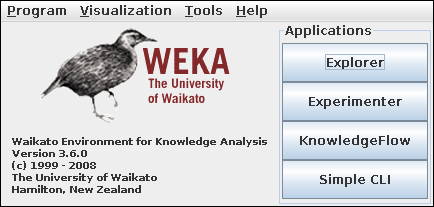
\includegraphics[width=1\hsize]{image201003/weka0.png}
 \caption{Weka 起動メニュー}
 \end{center}
\end{minipage}
\begin{minipage}{0.5\hsize}
 \begin{center}
 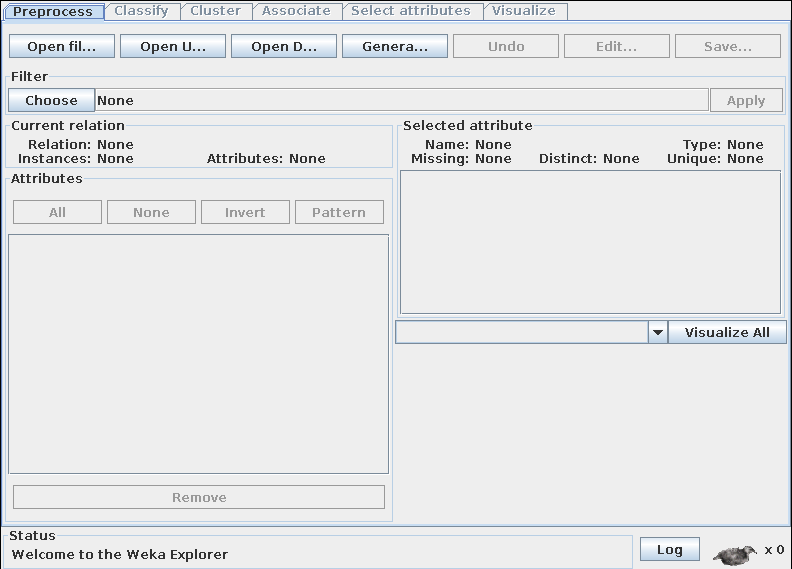
\includegraphics[width=1\hsize]{image201003/weka1.png}
 \caption{Weka Explorer}
 \end{center}
\end{minipage}
\end{figure}

\subsubsection{Weka で扱うデータフォーマット}

Weka では、ARFF(Attribute-Relation File Format)というフォーマットのテキ
ストファイルを入力データとして扱います。
\index{arff}

データフォーマットは次のようになります。

\begin{commandline}
@relation 名前 ←データ全体の名前を指定
@attribute 属性名 属性の型 ←データの属性。1つ目の引数は属性名、2つめの引数は属性データの型
@attribute 属性名 属性の型
:
:
@data ←データ領域の宣言
データ,データ,…,データ ←CSV 形式でデータを記述
\end{commandline}

\begin{itemize}
\item @relation はデータ全体の名前を指定します。
\item @attribute はデータの属性を表し、1つ目の引数は属性名、2つめの引数
      は属性データの型を表します。
\item @attribute のデータ型には、numeric, real, integer, string, date型
      を使えます。
      \begin{itemize}
       \item numeric は real か integer を指定できます。
       \item real は実数を指定できます。
       \item integer は整数を指定できます。
       \item string は文字列を指定できます。
       \item date 型は日時で、デフォルトは''yyyy-MM-dd'T'HH:mm:ss''とい
	     う書式です。
      \end{itemize}
 \item @data データ領域の宣言です。
       \begin{itemize}
	\item その次の行から CSV 形式でデータを記述します。
	\item @attribute 行で上から設定した順に CSV の一行での左から右へ
	      の各データとなります。
       \end{itemize}
\end{itemize}

昨年の11月の勉強会で GNU R で扱った光熱費のデータと、気象庁が公開してい
る気温、降水量などの気象データ\footnote{\url{http://www.data.jma.go.jp/obd/stats/etrn/index.php}}を使ってみます。

まず、CSV で以下のように記述したとします。
\begin{commandline}
"年","月","降水量合計(mm)","平均日平均気温(℃)","平均日最高気温(℃)","平均日最低気
温(℃)","平均風速(m/s)","最大風速(m/s)","日照時間(h)","電気使用量(kWh)","電気使用
量(kWh)/日","料金(円)/日","合計料金","ガス使用量(m3)","ガス使用量(m3)/日","料金(
円)/日","合計料金"
2007,1,50,6,10.8,1.1,1,5,188.9,234,6.88235294117647,161.235294117647,5482,9,0.333333333333333,80.962962962963,2186
2007,2,44,7.3,12.6,1.9,1.3,6,198.1,198,7.07142857142857,168.071428571429,4706,9,0.321428571428571,87.7142857142857,2456
(snip)
\end{commandline}

これは、ARFF フォーマットでは以下のようになります。

\begin{commandline}
@relation 降水量・気温(府中市)と電気代、ガス代の関係について

@attribute 年 real
@attribute 月 real
@attribute 降水量合計(mm) real
@attribute 平均日平均気温(℃) real
@attribute 平均日最高気温(℃) real
@attribute 平均日最低気温(℃) real
@attribute 平均風速(m/s) real
@attribute 最大風速(m/s) real
@attribute 日照時間(h) real
@attribute 電気使用量(kWh) real
@attribute 電気使用量(kWh)/日 real
@attribute 料金(円)/日 real
@attribute 合計料金 real
@attribute ガス使用量(m3) real
@attribute ガス使用量(m3)/日 real
@attribute 料金(円)/日 real
@attribute 合計料金 real

@data
2007,1,50,6,10.8,1.1,1,5,188.9,234,6.88235294117647,161.235294117647,5482,9,0.333333333333333,80.962962962963,2186
2007,2,44,7.3,12.6,1.9,1.3,6,198.1,198,7.07142857142857,168.071428571429,4706,9,0.321428571428571,87.7142857142857,2456
(snip)
\end{commandline}

\subsubsection{ARFF をロードする}

先ほど用意した kohnetsu.arff をロードしてみましょう。Preprocess タブの
Open File ボタンを押します。ダイアログが表示されるので、kohnetsu.arff を
指定します。(\fgref{fig:wekaarffload})

ARFF ファイルを読み込むと\fgref{fig:wekaarffread}のようになります。UTF-8 エンコードであれば、
ご覧のとおり日本語も正常に読み込めます

\begin{figure}[H]
 \begin{minipage}{0.5\hsize}
  \begin{center}
   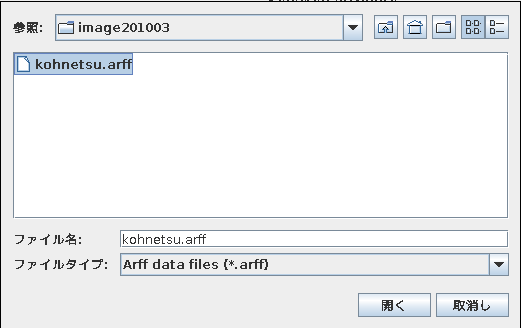
\includegraphics[width=0.9\hsize]{image201003/weka2.png}
   \caption{ARFF ファイルをロードする}
   \label{fig:wekaarffload}
  \end{center}
 \end{minipage}
 \begin{minipage}{0.5\hsize}
  \begin{center}

   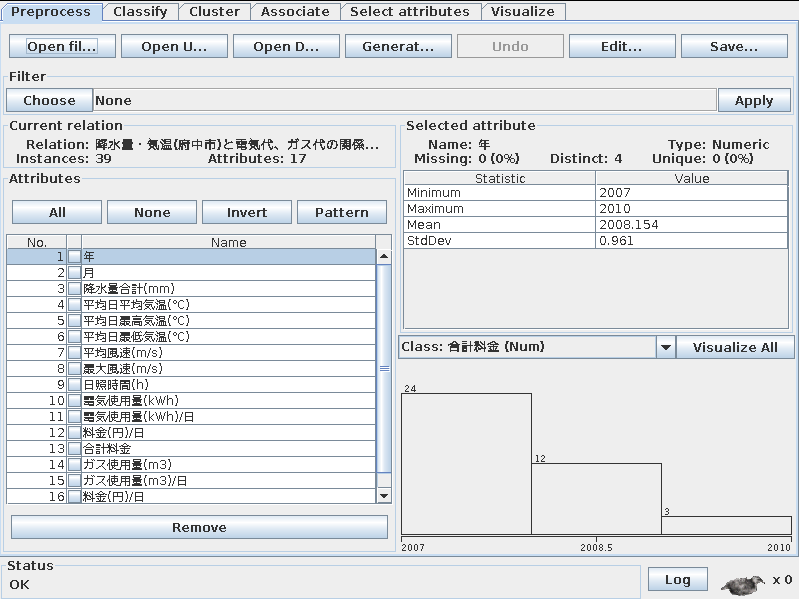
\includegraphics[width=0.9\hsize]{image201003/weka3.png}
   \caption{ARFF からデータを読み込んだ結果}
   \label{fig:wekaarffread}
  \end{center}
 \end{minipage}
\end{figure}

\subsubsection{可視化してみる}

それでは読み込んだデータを可視化してみましょう。Visualize タブをクリック
すると\fgref{fig:wekavisualize}のようなマトリックスが表示されます。

適当に開いてみます。Y 軸に一日の平均気温の月平均(℃)と、 X 軸に一日あた
りの電気使用量(kWh)を取って見てみると\fgref{fig:wekavisualizedetail}のようになります。

\begin{figure}[H]
 \begin{minipage}{0.5\hsize}
\begin{center}
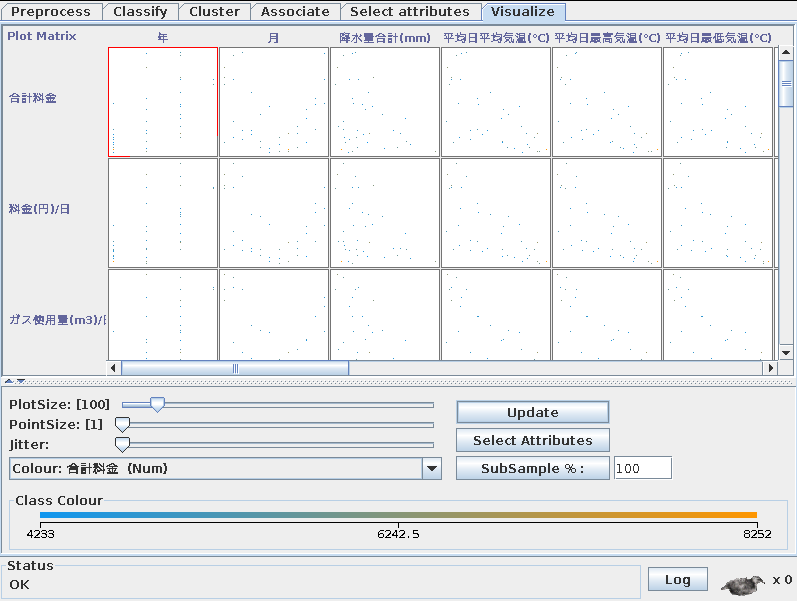
\includegraphics[width=1\hsize]{image201003/weka4.png}
\caption{Visualize 画面}
\label{fig:wekavisualize}
\end{center}
\end{minipage}
\begin{minipage}{0.5\hsize}
 \begin{center}
 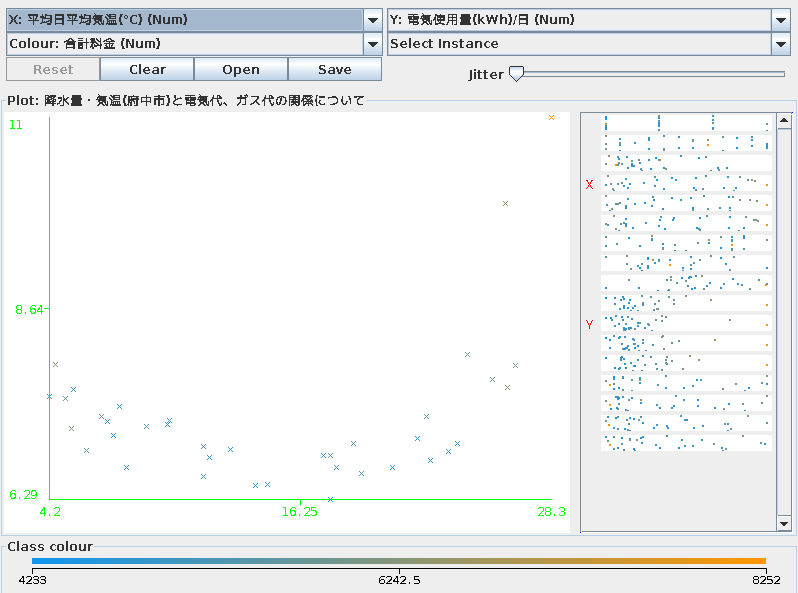
\includegraphics[width=1\hsize]{image201003/weka5.png}
 \caption{Visualize 詳細画面}
\label{fig:wekavisualizedetail}
 \end{center}
\end{minipage}
\end{figure}


\subsubsection{分類してみる}

次に分類してみます。Classify タブ → Choose ボタンを押し、表示されたツリー
からMultilayer Perceptron (ニューラルネットワークによる分類)を選択します。
次に、(Num)平均日平均気温(℃) を目的関数として選択します。
\index{neural network}

\begin{figure}[H]
\begin{center}
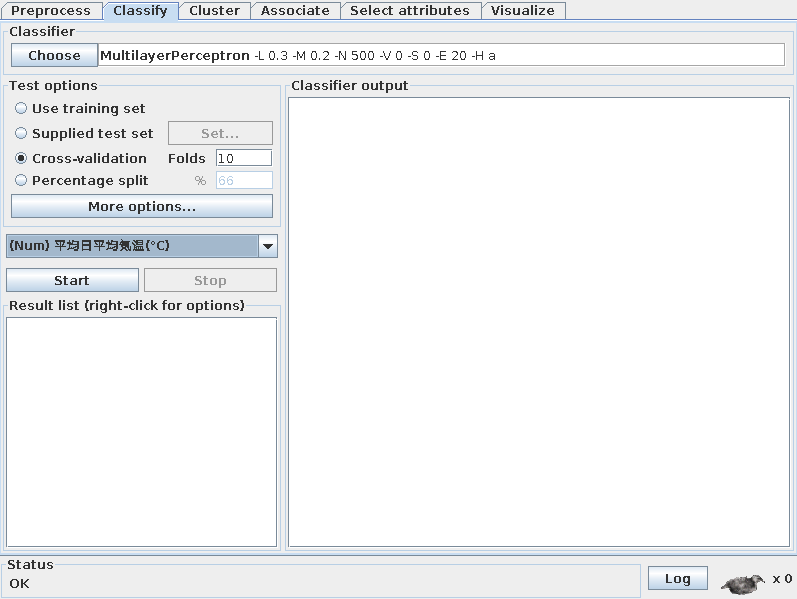
\includegraphics[width=0.6\hsize]{image201003/weka6.png}
\caption{Classify 画面}
\end{center}
\end{figure}

Start ボタンをクリックすると分類が実行され、結果が表示されます。

\begin{figure}[H]
\begin{center}
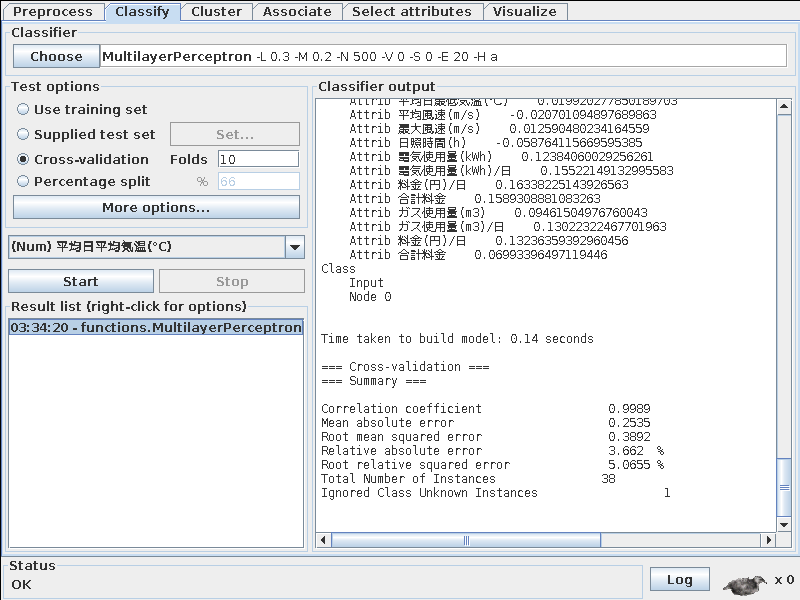
\includegraphics[width=0.6\hsize]{image201003/weka7.png}
\caption{Classify 結果}
\end{center}
\end{figure}

\subsubsection{予測してみる}

実は、kohnetsu.arff の最後の行(2010年3月のデータ)は、ほとんどの項目を'?'を入力
しています。

\begin{commandline}
2010,3,?,?,?,?,?,?,?,?,?,?,?,?,?,?,?
\end{commandline}

これはまだ今月のデータが出ていないからです。それでは、これらを予測してみ
ます。先ほどの Classify タブの画面で More options をクリックし、Output
predictions のチェックを入れ、OK を押します。

\begin{figure}[H]
\begin{center}
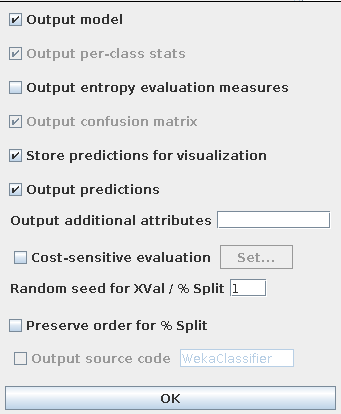
\includegraphics[width=0.4\hsize]{image201003/weka8.png}
\caption{Classify の More Options ダイアログ}
\end{center}
\end{figure}

Start を実行すると、予測結果が表示されます。actual が実データで
predicted が予測結果です。今回見たいのは、3月の平均日平均気温です。
actual が ? になっている行の、predicted の値を見ると、15.436 となってい
ます。過去読み込ませたデータからニューラルネットワークでの分析して予測し
た結果、おそらく一日あたりの平均気温は 15.4 ℃ になるという予測です。来
月、気象庁の統計データが更新されたら確認してみましょう。

\begin{figure}[H]
\begin{center}
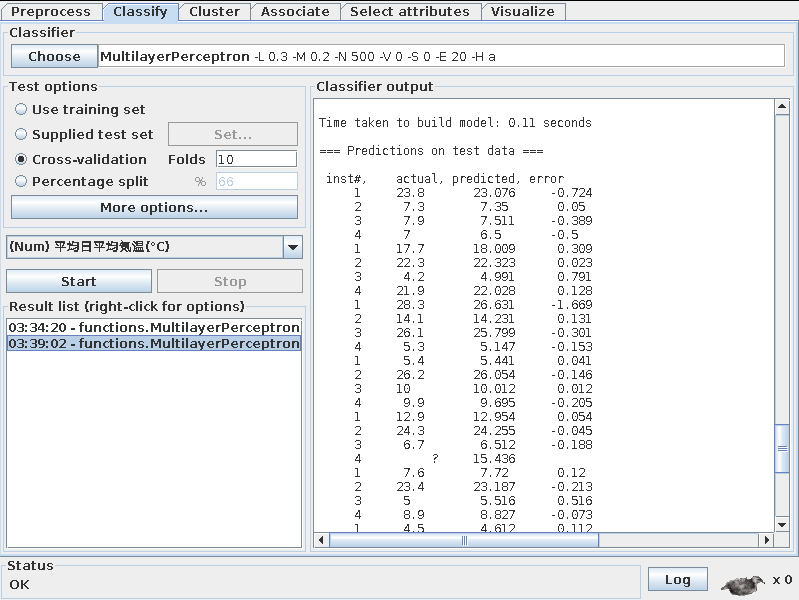
\includegraphics[width=0.6\hsize]{image201003/weka9.png}
\caption{予測結果}
\end{center}
\end{figure}

\subsection{まとめ}

なんとなく使えそうな気がしたでしょうか。私はこれで毎月のガス代、電気代、
さらには水道代の予測をして、給与日前日の予算計画に利用していこうと思いま
す。仕事でも、企画上の裏付けデータの分析、予測などにも使えそうですね。

\subsection{参考文献}
\begin{itemize}
 \item \url{http://www.ilibrary.jp/MOTtextBooks/text/weka.pdf}
 \item \url{http://web.sfc.keio.ac.jp/~soh/dm03/}
 \item \url{http://www1.doshisha.ac.jp/~mjin/R/23.pdf}
 \item \url{http://weka.wikispaces.com/ARFF}
\end{itemize}

%-------------------------------------------------------------------------------
% from debianmeetingresume201003.tex
\dancersection{Debian で libfftw を使ってみる}{上川純一}
%-------------------------------------------------------------------------------
\index{fftw}
\index{FFT}
\index{DFT}
\index{libfftw}
\index{libsndfile}

\subsection{はじめに}

DebianでFFTを取り扱うCのアプリケーションを書いてみたいと思うことはあり
ませんか?今日は音声データを分析してみましょう。

wav ファイルを入力として受け取り、FFTを実行してその結果を表示するアプリケー
ションを作成してみます。

\subsection{インストール}

libfftw3 をインストールします。
あと、音声ファイルをロードするために sndfile1 を利用します。

\begin{commandline}
$ apt-get install libfftw3-dev libsndfile1-dev
\end{commandline}
%$

\subsection{実験対象の準備:簡単なsine波を作成する}

まず、テスト用にFFTの結果が予想できるデータを作成してみます。
ここでは 440Hz のきれいなサイン波を作成しています。

\begin{equation*}
 data(x) = sin (\frac{2 \pi 440 x}{44100} ) 
\footnote{sin は radian}
\end{equation*}

\begin{commandline}
/*BINFMTC: -lsndfile -lm

  Create a sine wave at 44.1kHz for 1 second called sine.wav
 */
#include <stdlib.h>
#include <stdio.h>
#include <sndfile.h>
#include <math.h>

int create_sine(const char* filename, int size, double frequency)
{
  SF_INFO sfinfo = {
    .frames = size,
    .samplerate = 44100,
    .channels = 1,
    .format = SF_FORMAT_WAV | SF_FORMAT_PCM_16,
    .sections = 0,
    .seekable = 0
  };
  SNDFILE* s = sf_open(filename, SFM_WRITE, &sfinfo);
  double* data = malloc(sizeof(double) * size);
  int i;

  for (i=0; i < size; ++i)
    {
      data[i] = sin(frequency * 2.0 * M_PI * i / 44100.0);
    }

  sf_writef_double(s, data, size);
  sf_close(s);
  return 0;
}

int main()
{
  return create_sine("sine.wav", 44100, 440.0);
}
\end{commandline}

\subsection{実験対象の準備:複雑な入力値例の準備}

テスト用の入力値として、適当な wav ファイルを用意しましょう。

今回は手元で、aeolus というオルガンシミュレータを起動し、 
jack で接続させ、ecasound を jack 入力に
対して待機させ、qjackctl で接続させて収録しました。

それなりに長い時間録音したデータから 16-bit mono の PCM データ1秒分を切り
出して実験用データを作成しました。

\begin{commandline}
$ qjackctl &
$ aeolus &
$ vkeybd &
$ ecasound -i jack -o test.wav
ctrl-C で中断
$ sweep test.wav # 適当に編集
$ file ra-mono.wav  # 切り出した結果を確認
ra-mono.wav: RIFF (little-endian) data, WAVE audio, Microsoft PCM, 16 bit, mono 44100 Hz
\end{commandline}
%$

\subsection{FFTWを使って wav ファイルを処理してみる}

sndfile と fftw3 を使ってフーリエ変換して出力をダンプしてみましょう。サン
プルコードは sndfile を使い double の配列にwavファイルの中身を展開して、
その内容を fftw に渡して処理しています。double の値は各 1/44100 秒の瞬間
における空気の圧力を表しているようです。

\begin{commandline}
/*BINFMTC: -lsndfile -lfftw3 -lm
 */

#include <stdlib.h>
#include <stdio.h>
#include <sndfile.h>
#include <math.h>
#include <complex.h>
#include <fftw3.h>

/*
  process with FFTW
 */
void study_sound(double* data, int size)
{
  fftw_complex* spectrum;
  fftw_plan p;
  int i;

  spectrum = (fftw_complex*) fftw_malloc(sizeof(fftw_complex) * (size / 2 + 1));
  p = fftw_plan_dft_r2c_1d(size, data, spectrum, FFTW_ESTIMATE);

  /* process with FFTW */
  fftw_execute(p);

  /* dump output in CSV format */
  printf("i,abs,arg\n");
  for (i=0; i<(size/2+1); ++i) {
    printf("%i,%f,%f\n", i,
	   cabs(spectrum[i]),
	   carg(spectrum[i]) / 2.0 / M_PI * 360.0);
  }
  fftw_destroy_plan(p);
  fftw_free(spectrum);
}

/*
  Process wav file.

  @return 1 on failure, 0 on success.
*/
int process_wav_file(const char* filename, int size)
{
  SF_INFO sfinfo = {0, 0, 0, 0, 0, 0};
  SNDFILE* s = sf_open(filename, SFM_READ, &sfinfo);
  double* data = malloc(sizeof(double) * size);

  if (!s || !data)
    {
      fprintf(stderr,
	      "Something went wrong opening the file or allocating memory\n");
      return 1;
    }
  if (sfinfo.channels != 1)
    {
      fprintf(stderr,
	      "Please give me monaural audio data\n");
      return 1;
    }

  /* Read wav file into an array of double */
  sf_readf_double(s, data, size / sfinfo.channels);
  study_sound(data, size / sfinfo.channels);
  sf_close(s);
  return 0;
}

int main(int argc, char** argv)
{
  process_wav_file(argv[1], atoi(argv[2]));
  return 0;
}
\end{commandline}

実行してみます。

\begin{commandline}
$ ./sndfile-fftw.c sine.wav 44100 > sine.csv
$ ./sndfile-fftw.c ra-1sec.wav 44100 > ra.csv
\end{commandline}
%$

\subsection{出力を確認してみる}

CSVファイル形式でデータが出力されました。
簡単にグラフを作成するためのツールとしてここではRを使ってみます。

\begin{commandline}
$ R
> sine <- read.csv("sine.csv")
> ra <- read.csv("ra.csv")
> postscript("sine.eps", horizontal=FALSE, height=3, width=3)
> plot(sine$i, sine$abs, xlim=c(400,500), ylim=c(0,22000), type="l")
> dev.off()
> postscript("ra.eps", horizontal=FALSE, height=3, width=3)
> plot(ra$i, ra$abs, xlim=c(0,2000), ylim=c(0,100), type="l")
> dev.off()
\end{commandline}

\fgref{fig:wave-sine}の440Hz のサイン波を処理した結果を見てみると、440
Hz あたりにグラフの突起があるのが見て取れます。

しかし、実際にオルガン音を処理した結果の\fgref{fig:wave-ra}を見てみると、
グラフに突起が多数あって、結構複雑です。そのまま簡単に処理させてくれはし
なさそうです。

\begin{figure}[ht]
\begin{center}
 \begin{minipage}{0.4\hsize}
 \begin{center}
  \includegraphics{image201003/sine.eps}
 \end{center} 
 \label{fig:wave-sine}
 \caption{440Hz のサイン波}
 \end{minipage}
 \begin{minipage}{0.4\hsize}
 \begin{center}
  \includegraphics{image201003/ra.eps}
 \end{center} 
 \label{fig:wave-ra}
 \caption{ラをaeolusで適当に演奏した音}
 \end{minipage}
\end{center}
\end{figure}

%-------------------------------------------------------------------------------
% from debianmeetingresume201003.tex
\dancersection{man-db を深追いした}{日比野 啓}
%-------------------------------------------------------------------------------
\index{man-db}
\index{groff}

\subsection{日本語のmanが変}

こんな感じ\\
\begin{wrapfigure}{r}{80mm}
\includegraphics[width=75mm]{image201003/manls.eps}
\end{wrapfigure}


日本語の文字の表示幅がアルファベットと同じだと判定されてしまっているので、
結果的に日本語で書かれた行の長さが倍ぐらいになってしまっています。

\subsection{解はgroffにあり}

\subsubsection{そもそもroffってどういうもの?}

簡単に言えば、タイプライターのようなものです。
いろいろなデバイスに対して印字を行なうことができるシステムになっていますが、
manでは文字端末に文字の幅と高さを考慮しながら印字をしていきます。

\subsubsection{roff文字幅の指定}

以前のバージョンのgroffでは日本語の文字の表示幅がアルファベットの倍であることを
unicodeのcode pointの範囲で設定してありました。
groffにはもともとcode pointの範囲で文字の幅を指定する機能が無いため、
その機能の追加と日本語文字の表示幅を倍にするパッチがあててありました。

更新されたバージョンにおいては日本語対応のパッチが当たらなくなってしまっていますが、
やはり同様の対処を行なう必要がありそうです。

% 最近はその日本語の文字の幅の指定が柔軟になったようですが、正しい設定がさ
% れていないようです。

% =======================================================================
% from debianmeetingresume201002.tex
\dancersection{DebianのOCaml環境で開発する関数型言語インタプリタ}{日比野 啓}
\index{functional programming}
\index{OCaml}
\index{Haskell}
% =======================================================================

\subsection{OCamlはどんな言語}

静的型の型推論言語というのが今の私の認識です。
関数型言語らしい機能が注目されますが、それ以外のスタイルも良く利用されます。

ここではこの記事を読みすすめるにあたって必要そうなOCamlの機能について簡単に紹介します。

\subsubsection{値}

以下、対話環境の入出力を前提に話をすすめます。

ocaml-interpパッケージの /usr/bin/ocaml が対話環境のプログラムです。

\verb|# | は対話環境のプロンプトです。
ユーザーの入力の終わりを対話環境に認識してもらうために \verb|;;|を入力します。
なので対話環境の\verb|# |プロンプトの後ろから\verb|;;|までがユーザーの入力です。
\verb|- :|から始まる内容は対話環境の出力です。

\begin{commandline}
# 1;;
- : int = 1
# "abc";;
- : string = "abc"
# (1, "abc");;
- : int * string = (1, "abc")
# (1, ("abc", 2), 3);;
- : int * (string * int) * int = (1, ("abc", 2), 3)
# [ "a"; "b"; "c"];;
- : string list = ["a"; "b"; "c"]
# "a" :: "b" :: "c" :: [];;
- : string list = ["a"; "b"; "c"]
\end{commandline}

値を表す式を入力すると対話環境は型の名前と値を出力しています。
\verb|1|は\verb|int|型、\verb|"abc"|は\verb|string|型となっています。
対話環境に式を入力したので評価が行なわれ、その結果としての出力です。

\verb|(1, ("abc", 2), 3)|のようにコンマで区切って括弧でくくった値はタプルです。
値と値の組を表現できます。型の名前は \verb|*|で連ねます。任意の型の値を組にできる強力な機能です。

\verb|[ ]|でリストを表現することができます。また、\verb|::|はlispでいうところのconsです。
リストの要素は全て同じ型である必要があります。

\subsubsection{レコードとバリアント}

次は値を表現する前にあらかじめ型の定義が必要であるような値です。

\begin{commandline}
# type vec_2d = { x : int; y : int };;
type vec_2d = { x : int; y : int; }
# { x = 1; y = 2 };;
- : vec_2d = {x = 1; y = 2}
# type int_or_string_or_none = I of int | S of string | N;;
type int_or_string_or_none = I of int | S of string | N
# I 3;;
- : int_or_string_or_none = I 3
# S "hello";;
- : int_or_string_or_none = S "hello"
# N;;
- : int_or_string_or_none = N
\end{commandline}

一つ目の例はレコードです。Cの構造体のようなもので、フィールド名とフィールドの型を定義に記述します。
\verb|vec_2d|というレコードの型を定義して、\verb|{ x = 1; y = 2 }|という値を評価させました。

二つ目はバリアントあるいは代数データ型と呼ばれている種類の型です。
\verb|int_or_string_or_none|という型を定義していて、
その値は Iというタグの付いたint か Sというタグの付いたstring か N というタグ のどれかということです。
このタグのことを{\bf コンストラクタ}と呼びます。

バリアントは再帰的な定義も可能で、この機能で簡単に木構造を表現できます。

\begin{commandline}
# type str_tree = Leaf of string | Tree of (str_tree * str_tree);;
type str_tree = Leaf of string | Tree of (str_tree * str_tree)
# Leaf "abc";;
- : str_tree = Leaf "abc"
# Tree (Leaf "a", Tree (Leaf "b", Leaf "c"));;
- : str_tree = Tree (Leaf "a", Tree (Leaf "b", Leaf "c"))
\end{commandline}

\subsubsection{関数}

次は関数を表現する値です。

\begin{commandline}
# (fun x -> x + 1);;
- : int -> int = <fun>
# (fun x -> x);;
- : 'a -> 'a = <fun>
\end{commandline}

\verb|(fun x -> x + 1)|は関数です。
型が\verb|int -> int|と出力されていますが、
これはintを受けとってintを返す関数という意味です。
\verb|+|の引数はintとintなので結果として\verb|x|は\verb|int|、
\verb|fun x -> x + 1| は \verb|int -> int|というように型の推論が行なわれています。

二番目の\verb|(fun x -> x)|も関数です。
型が\verb|'a -> 'a|と出力されていますが、
これは何かある型の値を受けとって、同じ型の値を返す関数という意味です。
この \verb|'a -> 'a| の関数は任意の型に対して適用が可能なので、
全ての型についてこの関数が定義されている(\verb|int -> int| も \verb|string -> string| も ... etc)のと同様の効果があります。
このような型を多相型と呼びます。

\subsubsection{束縛}

\verb|let|を使って値を変数に束縛します。
以下は\verb|v|にたいして整数を\verb|f|に対して関数を束縛しています。

\begin{commandline}
# let v = 123;;
val v : int = 123
# v;;
- : int = 123
# let f x y = (x + y) * (x - y);;
val f : int -> int -> int = <fun>
# f 5 3;;
- : int = 16
\end{commandline}

\subsubsection{パターン照合}

OCamlは値の構造を分解しつつ変数を束縛することができます。
次の例ではタプルを分解して束縛を行なっています。

\begin{commandline}
# let (x, y) = (2, 3 + 4);;
val x : int = 2
val y : int = 7
# let (a, (b, c)) = (1, (2, 3));;
val a : int = 1
val b : int = 2
val c : int = 3
\end{commandline}

\verb|match ... with|を使用すると、構造分解を試みつつ条件分岐することができます。

関数\verb|len|はリストが空かどうかを判定しながら再帰しています。
束縛の定義時に自身の定義を使用するときには\verb|let|ではなく\verb|let rec|を使います。

関数\verb|what|は先程定義したバリアント\verb|int_or_string_or_none|の値の種類によって返す文字列を変えています。

関数\verb|get_int|は\verb|int_or_string_or_none|がintのときだけSome intを返し、そうでないときは None を返します。
'a option は組み込みの型で、ある型の値が有るかあるいは無いかを表現できるバリアントです。

\begin{commandline}
# let rec len ls = match ls with [] -> 0 | x :: rest -> 1 + len rest;;
val len : 'a list -> int = <fun>
# len [1; 2; 3];;
- : int = 3
# let what v = match v with I _ -> "int" | S _ -> "string" | N -> "none";;
val what : int_or_string_or_none -> string = <fun>
# what (S "abc");;
- : string = "string"
# what N;;
- : string = "none"
# let get_int v = match v with I i -> Some i | _ -> None ;;
val get_int : int_or_string_or_none -> int option = <fun>
# get_int N;;
- : int option = None
# get_int (I 10);;
- : int option = Some 10
\end{commandline}

\subsubsection{モジュール}

プログラムの規模がおおきくなってくると名前空間が重要になってきます。
OCamlにはmoduleの機能があり名前空間を分けることができます。
あるコンパイル単位がxyz.mlというファイル名だった場合、
その中の定義はXyzというmoduleの中に配置されます。
モジュール内にたとえばabcという名前があった場合、
公開されていれば他のコンパイル単位のファイルからも Xyz.abc という名前でアクセスすることができます。

\begin{commandline}
(* xyz.ml *)
let abc = "abc"
...


(* 他のファイル *)
... Xyz.abc ...
\end{commandline}

moduleの中にさらにmoduleを定義することもできます。
xyz.mlの中に作ったmodule SubXyzは、Xyz.SubXyzという名前のmoduleです。

定義済みのモジュールを使ってmoduleを定義することもできます。
組み込みのmoduleであるListを使って Xyz.L を定義しています。

\begin{commandline}
(* xyz.ml *)
module SubXyz =
  struct
  ...
  end

module L = List
\end{commandline}


\subsection{関数型言語のインタプリタの簡単な作りかた}

関数型言語とは何でしょうか。
ここでは関数を値としてあつかえる言語ということにして、
そのような言語のインタプリタを作る話をします。

\subsubsection{環境を渡すナイーブなインタプリタ実装}
\label{sec:envmach}

\paragraph{letの環境} \ 

例えば以下のようなプログラムを考えます。

\begin{commandline}
;; scheme function
(define (f)
  ;; env A
  (let ((x 1) (y 2) (z 3))
    ;; env B
    (let ((y 4))
      ;; env C
      (let ((z 5))
	;; env D
	(+ x y z)))))
\end{commandline}

\begin{commandline}
(* OCaml function *)
let f () =
  (* env A *)
  let (x, y, z) = (1, 2, 3) in
    (* env B *)
  let y = 4 in
    (* env C *)
  let z = 5 in
    (* env D *)
    x + y + z
\end{commandline}

変数の値の解決のためのテーブルを環境(environment)と呼ぶことにして、
次の図ような構造になっていると考えてみます。
変数の検索は上から下に行なわれるとすると、
それぞれのコメントの位置の環境は矢印の位置を参照していると考えてよいはずです。

 \includegraphics[height=0.3\hsize]{image201002/caml-env00.eps}\label{fig:env00}

\paragraph{関数呼び出しにおける環境} \ 

さらに以下のようなプログラムを考えます。

\begin{commandline}
(define (f x y)
  ;; env f
  (* x y 2))

;;env X

(let ((x 1) (y 2))
  (define (g)
    ;; env g
    (f 3 4))
  (g))

;;; may be another call of (f x y)
\end{commandline}

\begin{commandline}
let rec f x y =
  (* env f *)
  x * y * 2

(* env X *)

let (x, y) = (1, 2)
let rec g () =
  (* env g *)
  f 3 4

let v = g ()

(* may be another call of f x y *)
\end{commandline}

するとそれぞれのコメントの位置の環境は\fgref{fig:caml-env005}のようにな
っているはずです。

\begin{figure}[h]
 \centering
 \includegraphics[height=0.25\hsize]{image201002/caml-env005.eps}
 \caption{コメントの位置の環境}
 \label{fig:caml-env005}
\end{figure}



ここで環境Xは同じ環境なので、共有させることにすると次のような構造を考えることができます。
ここで注意する必要があるのは、環境fは関数fが呼び出される度に異なるということです。
fの定義位置である環境Xは共通ですが、環境fは関数fが呼び出される度に環境Xを指す環境を伸長する必要があります。

 \includegraphics[height=0.5\hsize]{image201002/caml-env01.eps}

\paragraph{クロージャの環境} \ 

以下のようなプログラムを考えます。

\begin{commandline}
(define h
  (let ((x 1) (y 2))
    ;; env c
    (let ((f (lambda (z)
               ;; env l
	       (+ x y z))))
      f)))

;; env X

(h 3)
;;; may be another call of (h x)
\end{commandline}

\begin{commandline}
let rec h =
  let (x, y) = (1, 2) in
  (* env c *)
  let f z =
    (* env l *)
    x + y + z
  in f

(* env X *)

let v = h 3
(* may be another call of h x *)
\end{commandline}

関数が変数hに束縛されています。
しかもhはx, yを束縛しているletの外側にあるにもかかわらず、
呼び出した際にはx, yの値を評価します。

このletのような機能をレキシカルスコープと呼び、
またこのような関数をレキシカルクロージャ(lexical closure)あるいは単にクロージャ(closure)と呼びます。

上の例での環境を考えてみると次のような構造になっているはずです。

 \includegraphics[height=0.5\hsize]{image201002/caml-env015.eps}

hに束縛されているclosureはあきらかに環境cを知っている必要があります。
なぜなら呼び出し時には環境cを指す環境を生成しなければならないからです。
したがってclosureは以下のような構造になっていると考えることができます。
envはclosureの定義位置の環境でargsは仮引数リストそしてbodyは関数本体の式です。

 \includegraphics[height=0.4\hsize]{image201002/caml-env02.eps}

式の評価に必要な環境を評価器内で渡しながら、
letや関数呼び出しの際には環境を伸長する方針を取ると、
比較的簡単にインタプリタを実装することができます。
また、環境を保持する構造を考えればclosureを実現することもできます。

 参考資料: \verb|http://www.sato.kuis.kyoto-u.ac.jp/~igarashi/class/isle4-05w/text/eopl003.html|

\subsection{OCamlでのlexingとparsing - ocamllexとocamlyacc}

\subsubsection{ocamllex}

ocamllexはOCamlに付属している字句解析関数生成器(lexer generator)で、
OCamlから呼び出せるlexerを生成してくれます。
以下のようにC言語でもおなじみの lex, flex と似たような使用感になっています。

\begin{commandline}

{
  (* header *)
  (* Lexingのルール部分で参照したい内容をOCamlで書く *)
}

(* 文字列パターンの定義 *)

(* 字句解析(lexing)のルール記述 *)

{
  (* trailer *)
  (* ルール部分で生成された関数を参照する内容をOCamlで書く *)
}

\end{commandline}

\subsubsection{ocamlyacc}

同様に、ocamlyaccはOCamlに付属している構文解析関数生成器(parser generator)で、
OCamlから呼び出せるparserを生成してくれます。
こちらもやはり、以下のように yacc, bison と似たような使用感になっています。

\begin{commandline}

%{
  (* header *)
  (* 構文木生成処理で参照したい内容をOCamlで書く *)
%}
  /* declarations */
  /* 終端記号の型や構文木のrootの宣言 */
%%
  /* rules */
  /* 文脈自由文法と構文木生成処理を記述 */
%%
  (* trailer *)
  (* 生成されたparserの関数を参照する内容をOCamlで書く *)

\end{commandline}

\subsubsection{ocamllexとocamlyaccの使用例}

ocamllexとocamlyaccを併用する場合には、
ocamlyaccで生成させたparserの終端記号の定義を
lexerから参照させるようにするのがもっとも単純な使い方です。

以下がS式parserを生成させる例です。
sParser.mlyをocamlyaccで処理するとsParser.mlが生成され、
sLexer.mllをocamllexで処理するとsLexer.mlが生成されます。

\par
\paragraph{sParser.mly}
型ごとに終端記号を\%tokenで宣言し、
\%startと\%typeで構文木のrootとその型を指定します。
rootの名前が構文解析関数の名前になります。

yaccと同じ要領で文脈自由文法を記述していきます。
exprは真偽値、数値、文字列であるか、
あるいは、exprドット対またはexprを並べたもの を括弧で括ったものという定義になっています。

\begin{commandline}

%{
  (* sParser.mly *)

  module C = SCons

%}

/* File sparser.mly */
%token LPAREN RPAREN DOT_SYMBOL EOL BOOL_TRUE BOOL_FALSE
%token <SCons.s_int> INT
%token <float> FLOAT
%token <string> SYMBOL
%token <string> STRING
%start expr
%type <SCons.s_expr> expr
%%

expr_list:
  { C.Null }
| expr DOT_SYMBOL expr { C.Cons($1, $3) }
| expr expr_list { C.Cons($1, $2) }

expr:
| BOOL_TRUE               { C.Bool(true) }
| BOOL_FALSE              { C.Bool(false) }
| INT                     { C.Int($1) }
| FLOAT                   { C.Float($1) }
| SYMBOL                  { C.Symbol($1) }
| STRING                  { C.String($1) }
| LPAREN expr_list RPAREN { $2 }

\end{commandline}

% $ dummy comment

\par
\paragraph{sLexer.mll}
文字列パターンの定義では、正規表現の要領で文字集合や繰り返しの表現を利用して
定義を作り、letで名前を付けていきます。文字を '' でくくる以外は正規表現と同様です。
定義した文字列パターンをさらに別の文字列パターンに再利用することができます。

ルール記述の部分では、tokenの文字列パターンとtoken生成式をlexの要領で記述していきます。
キーワードruleの後の文字列がlexerの関数名になります。なのでここではその関数の名前はtokenです。

字句解析(Lexing)の過程における入力ファイル内の位置は、
lexbufのlex\_start\_pに記号(token)の開始位置が、
lex\_curr\_pにtokenの終了の次の位置が保持されています。
ocamllexデフォルトの動作ではpos\_cnum フィールドが更新されるのみなので、
ファイル先頭からのバイト数しかわかりません。
陽に行数の認識やタブによるカラム数の補正を行なう場合には、
lex\_start\_pとtokenをもとにlex\_curr\_pを修正してやる必要があります。
\footnote{次のlex\_start\_pは現在のlex\_curr\_pから引き継がれるので、
lex\_curr\_pを修正すれば十分です。}



\begin{commandline}
{
  (* sLexer.mll*)

  module LX = Lexing
  module P = SParser
  ... (* 中略 *)
  let fix_position lexbuf =
    let newline pos = {
      pos with
	LX.pos_lnum = pos.LX.pos_lnum + 1;
	LX.pos_cnum = pos.LX.pos_cnum + 1;
	LX.pos_bol = pos.LX.pos_cnum + 1;
    } in

    let tab pos = {
      pos with
	LX.pos_cnum = pos.LX.pos_cnum + 8 - (pos.LX.pos_cnum - pos.LX.pos_bol) mod 8
    } in

    let other pos = {
      pos with
	LX.pos_cnum = pos.LX.pos_cnum + 1
    } in

    let rec fix_pos_rec pos str =
      let len = (String.length str) in
	match (if len > 0 then (Some (str.[0]), String.sub str 1 (len - 1))
	       else (None, "")) with
	    (None, _) -> pos
	  | (Some '\n', rest) -> fix_pos_rec (newline pos) rest
	  | (Some '\t', rest) -> fix_pos_rec (tab pos) rest
	  | (Some _, rest) -> fix_pos_rec (other pos) rest
    in
    let _ = lexbuf.LX.lex_curr_p <- fix_pos_rec (LX.lexeme_start_p lexbuf) (LX.lexeme lexbuf) in
      ()
}

/* 文字列パターンの定義 */
let str_esc = '\\'
let double_quote = '"'
let str_escaped_char = str_esc _
let str_char = [^ '\\' '"']
let str = double_quote (str_char | str_escaped_char)* double_quote

let left_paren = '('
let right_paren = ')'
let space = [' ' '\t' '\n' '\r']+
let dot_symbol = '.'
let bool_true  = '#' 't'
let bool_false = '#' 'f'

let int = '-'? ['0' - '9']+
let float = '-'? ['0' - '9']+ '.' ['0' - '9']* | '-'? ['0' - '9']* '.' ['0' - '9']+
let symbol = [^ '"' '(' ')' ' ' '\t' '\n' '\r']+

/* lexingのルール記述 */
rule token = parse
  | left_paren      { P.LPAREN }
  | right_paren     { P.RPAREN }
  | space      { fix_position lexbuf; token lexbuf }
  | dot_symbol      { P.DOT_SYMBOL }
  | bool_true       { P.BOOL_TRUE }
  | bool_false      { P.BOOL_FALSE }
  | int      { expr_integer (LX.lexeme lexbuf) }
  | float    { P.FLOAT(Pervasives.float_of_string(LX.lexeme lexbuf)) }
  | symbol   { P.SYMBOL(LX.lexeme lexbuf) }
  | str      { fix_position lexbuf; P.STRING(expr_string(LX.lexeme lexbuf)) }
  | eof      { raise Eof }

\end{commandline}

%\pagebreak

\subsection{HaskellのLexing}

Haskellには
ブロックの開始や終了のtokenや式の区切りのtokenを省略することができる
layout ruleという機能があります。
そのため省略されたtokenをlexingの過程で補ってやる必要があります。

まず、通常と同様にlexingを行なってtoken列を生成し、
そのtoken列に規則に従ってtokenを補うというように、2段階の工程を行ないます。

\subsubsection{layoutなしのLexing}

\paragraph{lexer0.mll header部分} \ 

まずは.mllのheader部分です。

後からlayout ruleにおいて必要となるカラム数を数えあげる処理ために位置情報の修正を行なう関数(fix\_position)を定義しています。
また、Haskellの文字および文字列リテラルはリテラル内のルールが複雑度の高い仕様なので、
別のlexer(後述)を呼び出しつつ実際の文字列表現を構成する関数(decode\_char, decode\_string)を準備しています。


\paragraph{fix\_position 位置情報の修正} \ 
\begin{commandline}
{
  (* lexer0.mll header部分 *)
  module LX = Lexing
  module P = Parser
  ... (* 中略 *)
  let fix_position lexbuf =
    let newline pos =
      { pos with
          LX.pos_lnum = pos.LX.pos_lnum + 1;
          LX.pos_cnum = pos.LX.pos_cnum + 1;
          LX.pos_bol = pos.LX.pos_cnum + 1;
      } in

    let tab pos =
      { pos with
          LX.pos_cnum = pos.LX.pos_cnum + 8 - (pos.LX.pos_cnum - pos.LX.pos_bol) mod 8
      } in

    let other pos =
      { pos with
          LX.pos_cnum = pos.LX.pos_cnum + 1
      } in

    let rec fix_pos_rec pos str =
      let len = (String.length str) in
        match (if len > 0 then (Some (str.[0]), String.sub str 1 (len - 1))
               else (None, "")) with
            (None, _) -> pos
          | (Some '\n', rest) -> fix_pos_rec (newline pos) rest
          | (Some '\t', rest) -> fix_pos_rec (tab pos) rest
          | (Some _, rest) -> fix_pos_rec (other pos) rest
    in
    let _ = lexbuf.LX.lex_curr_p <- fix_pos_rec (LX.lexeme_start_p lexbuf) (LX.lexeme lexbuf) in
      ()
  ... (* 中略 *)
\end{commandline}

\pagebreak

\paragraph{decode\_char, decode\_string 文字および文字列デコーダー} \
\begin{commandline}
  ... (* 中略 *)
  let decode_cexpr cexpr =
    let fchar = String.get cexpr 0 in
    let escexp = String.sub cexpr 1 ((String.length cexpr) - 1) in
    let fmatch exp str = Str.string_match (Str.regexp exp) str 0 in
      if fchar = '\\' then
        match escexp with
            "NUL"   -> Some '\x00'
          | "SOH" | "^A"   -> Some '\x01'
          | "STX" | "^B"   -> Some '\x02'
        ... (* 中略 *)
          | "RS"  | "^^"   -> Some '\x1e'
          | "US"  | "^_"   -> Some '\x1f'
          | "SP"           -> Some ' '

          | "\\"           -> Some '\\'
          | "\""           -> Some '"'
          | "'"            -> Some '\''

          | "DEL"          -> Some '\x7f'

          | _ when fmatch "^[0-9]+$" escexp
              -> Some (Char.chr (int_of_string escexp))
          | _ when fmatch "^[xX][0-9a-zA-Z]+$" escexp 
              -> Some (Char.chr (int_of_string ("0" ^ escexp)))
          | _ when fmatch "^[oO][0-7]+$" escexp
              -> Some (Char.chr (int_of_string ("0" ^ escexp)))

          | _ -> None

      else Some fchar

  let decode_char lexbuf =
    let cstr = LX.lexeme lexbuf in
    let len = String.length cstr in
      match decode_cexpr (String.sub cstr 1 (len - 2)) with
          Some c -> c
        | None   -> failwith (F.sprintf "Unkown char expression %s" cstr)

  let decode_string lexbuf =
    let sexpr = LX.lexeme lexbuf in
    let len = String.length sexpr in
    let strlbuf = Lexing.from_string (String.sub sexpr 1 (len - 2)) in
    let rec decode result =
      match HsStr.char strlbuf with
          HsStr.Eos -> result
        | HsStr.Char cstr ->
            if cstr = "\\&" then decode (result ^ "&")
            else decode (result ^ 
                           match (decode_cexpr cstr) with
                               None -> failwith (F.sprintf "Unkown char expression '%s' in literal string" cstr)
                             | Some c -> (String.make 1 c))
        | HsStr.Gap g -> decode result
    in decode ""
}
\end{commandline}

% $ dummy comment

\pagebreak

\paragraph{lexer0.mll 文字列パターン定義部分} \ 

次に文字列パターンの定義です。

行数はちょっと多いですが、特に難しいところはありません。
問題のリテラル文字列ですが、リテラル文字列部分の文字列パターン自体は問題なく表現できています。
しかし、リテラルで表現される文字列自体を復元するのが複雑なので前記および後述のような準備が必要になります。

\begin{commandline}
/* lexer0.mll 文字列パターン定義部分 */
let special = ['(' ')' ',' ';' '[' ']' '`' '{' '}']

let space = ' '
let newline = ("\r\n"|['\n' '\r'])
let tab = '\t'

let dashes = '-' '-' '-'*

let ascSmall = ['a'-'z']
let small = ascSmall | '_'
let ascLarge = ['A'-'Z']
let large = ascLarge

let plus = '+'
let minus = '-'
let exclamation = '!'
let ascSymbol_nbs = [ '!' '#' '$' '%' '&' '*' '+' '.' '/' '<' '=' '>' '?' '@' '^' '|' '-' '~' ]
let ascSymbol = ascSymbol_nbs | '\\'
let symbol = ascSymbol

let ascDigit = ['0'-'9']
let digit = ascDigit

let octit = ['0'-'7']
let hexit = ascDigit | ['a'-'z' 'A'-'Z']

let decimal = (digit)+
let octal = (octit)+
let hexadecimal = (hexit)+

let exponent = ['e' 'E'] ['+' '-']? decimal
let float = decimal '.' decimal exponent? | decimal exponent

let graphic = small | large | symbol | digit | special | [':' '"' '\'']
let any = graphic | space | tab

let comment = dashes ((space | tab | small | large | symbol | digit | special | [':' '"' '\'']) (any)*)? newline

let whitechar = newline | space | tab
let whitestuff = whitechar | comment 
let whitespace = (whitestuff)+

(*
let lwhitechar = space | tab
let lwhitestuff = lwhitechar | comment 
let lwhitespace = (lwhitestuff)+
*)

let char_gr = small | large | ascSymbol_nbs | digit | special | [':' '"']
let str_gr  = small | large | ascSymbol_nbs | digit | special | [':' '\'']

let charesc = ['a' 'b' 'f' 'n' 'r' 't' 'v' '\\' '"' '\'']
let str_charesc = charesc | '&'
let cntrl = ascLarge | ['@' '[' '\\' ']' '^' '_']
let gap = '\\' (whitechar)+ '\\'
(* let gap = '\\' (lwhitechar | newline)+ '\\' *)

let ascii = ('^' cntrl) | "NUL" | "SOH" | "STX" | "ETX" | "EOT" | "ENQ" | "ACK"
  | "BEL" | "BS" | "HT" | "LF" | "VT" | "FF" | "CR" | "SO" | "SI" | "DLE"
  | "DC1" | "DC2" | "DC3" | "DC4" | "NAK" | "SYN" | "ETB" | "CAN"
  | "EM" | "SUB" | "ESC" | "FS" | "GS" | "RS" | "US" | "SP" | "DEL"

let escape = '\\' ( charesc | ascii | decimal | 'o' octal | 'x' hexadecimal )
let str_escape = '\\' ( str_charesc | ascii | decimal | 'o' octal | 'x' hexadecimal )

let char = '\'' (char_gr | space | escape) '\''
let string = '"' (str_gr | space | str_escape | gap)* '"'

let varid = small (small | large | digit | '\'')*
let conid = large (small | large | digit | '\'')*

let varsym = symbol (symbol | ':')*
let consym = ':' (symbol | ':')*

let modid = conid
\end{commandline}

% $ dummy comment

\pagebreak

\paragraph{lexer0.mll ルール記述部分} \ 

最後にルール記述です。

スペース、タブ、改行などを含んでいるwhitespaceやstringのところで
fix\_positionを呼んで位置情報を補正しています。
またcharやstringのリテラルから文字や文字列を構成するために
decode\_char, decode\_string を呼び出しています。

\begin{commandline}
(* lexer0.mll ルール記述部分 *)
rule token = parse
  | '('  { P.SP_LEFT_PAREN(loc lexbuf) }
  | ')'  { P.SP_RIGHT_PAREN(loc lexbuf) }
  | ','  { P.SP_COMMA(loc lexbuf) }
  | ';'  { P.SP_SEMI(loc lexbuf) }
  | '['  { P.SP_LEFT_BRACKET(loc lexbuf) }
  | ']'  { P.SP_RIGHT_BRACKET(loc lexbuf) }
  | '`'  { P.SP_B_QUOTE(loc lexbuf) }
  | '{'  { P.SP_LEFT_BRACE(loc lexbuf) }
  | '}'  { P.SP_RIGHT_BRACE(loc lexbuf) }
      (** special tokens *)

  | "case"     { P.K_CASE(loc lexbuf) }
  | "class"    { P.K_CLASS(loc lexbuf) }
  | "data"     { P.K_DATA(loc lexbuf) }
  | "default"  { P.K_DEFAULT(loc lexbuf) }
  | "deriving" { P.K_DERIVING(loc lexbuf) }
  | "do"       { P.K_DO(loc lexbuf) }
  | "else"     { P.K_ELSE(loc lexbuf) }
  | "if"       { P.K_IF(loc lexbuf) }
  | "import"   { P.K_IMPORT(loc lexbuf) }
  | "in"       { P.K_IN(loc lexbuf) }
  | "infix"    { P.K_INFIX(loc lexbuf) }
  | "infixl"   { P.K_INFIXL(loc lexbuf) }
  | "infixr"   { P.K_INFIXR(loc lexbuf) }
  | "instance" { P.K_INSTANCE(loc lexbuf) }
  | "let"      { P.K_LET(loc lexbuf) }
  | "module"   { P.K_MODULE(loc lexbuf) }
  | "newtype"  { P.K_NEWTYPE(loc lexbuf) }
  | "of"       { P.K_OF(loc lexbuf) }
  | "then"     { P.K_THEN(loc lexbuf) }
  | "type"     { P.K_TYPE(loc lexbuf) }
  | "where"    { P.K_WHERE(loc lexbuf) }
  | "_"        { P.K_WILDCARD(loc lexbuf) }
      (** reservedid *)

  | ".."       { P.KS_DOTDOT(loc lexbuf) }
  | ":"        { P.KS_COLON(loc lexbuf) }
  | "::"       { P.KS_2_COLON(loc lexbuf) }
  | "="        { P.KS_EQ(loc lexbuf) }
  | "\\"       { P.KS_B_SLASH(loc lexbuf) }
  | "|"        { P.KS_BAR(loc lexbuf) }
  | "<-"       { P.KS_L_ARROW(loc lexbuf) }
  | "->"       { P.KS_R_ARROW(loc lexbuf) }
  | "@"        { P.KS_AT(loc lexbuf) }
  | "~"        { P.KS_TILDE(loc lexbuf) }
  | "=>"       { P.KS_R_W_ARROW(loc lexbuf) }
      (** reservedop *)

  | "as"              { P.K_AS(loc lexbuf) }  (** maybe varid *)
  | "qualified"       { P.K_QUALIFIED(loc lexbuf) }  (** maybe varid *)
  | "hiding"          { P.K_HIDING(loc lexbuf) }  (** maybe varid *)
  | varid      { P.T_VARID(LX.lexeme lexbuf, loc lexbuf) }
  | conid      { P.T_CONID(LX.lexeme lexbuf, loc lexbuf) }
      (** identifiers or may be qualified ones *)

  | whitespace  { fix_position lexbuf; P.WS_WHITE(loc lexbuf) }  (** comment begining with dashes is not varsym *)
      (** white spaces *)

  | plus       { P.KS_PLUS(loc lexbuf) }  (** maybe varsym *)
  | minus      { P.KS_MINUS(loc lexbuf) } (** maybe varsym *)
  | exclamation  { P.KS_EXCLAM(loc lexbuf) } (** maybe varsym *)
  | varsym     { P.T_VARSYM(LX.lexeme lexbuf, loc lexbuf) }
  | consym     { P.T_CONSYM(LX.lexeme lexbuf, loc lexbuf) }
      (** symbols or may be qualified ones *)

  | modid '.' varid   { P.T_MOD_VARID(decode_with_mod lexbuf, loc lexbuf) }
  | modid '.' conid   { P.T_MOD_CONID(decode_with_mod lexbuf, loc lexbuf) }
  | modid '.' varsym  { P.T_MOD_VARSYM(decode_with_mod lexbuf, loc lexbuf) }
  | modid '.' consym  { P.T_MOD_CONSYM(decode_with_mod lexbuf, loc lexbuf) }
      (** qualified xx *)

  | char      { P.L_CHAR(decode_char lexbuf, loc lexbuf) }
  | string    { fix_position lexbuf; P.L_STRING(decode_string lexbuf, loc lexbuf) }

  | decimal | ('0' ['o' 'O'] octal) | ('0' ['x' 'X'] hexadecimal)
        { P.L_INTEGER(Int64.of_string(LX.lexeme lexbuf), loc lexbuf) }

  | float      { P.L_FLOAT(float_of_string(LX.lexeme lexbuf), loc lexbuf) }

  | eof        { P.EOF(loc lexbuf) }
  ... /* 以下略 */
\end{commandline}


\paragraph{hsStr.mll} \ 

文字列のlexerです。

ここでのtokenは文字列リテラル内の1文字の表現あるいはギャップ(gap)です。
Haskellでは1つの文字列リテラルを中断して、
間に空白や改行やコメントを記述した後に、再開することができます。
この空白や改行やコメントの部分がgapです。

ここで定義されたchar関数を利用してdecode\_string関数は文字列を構成していくようになっています。

\begin{commandline}
{
  (* hsStr.mll *)
  module LX = Lexing

  type ct =
      Char of string
    | Gap of string
    | Eos
}

let special = ['(' ')' ',' ';' '[' ']' '`' '{' '}']

let space = ' '
let newline = ("\r\n"|['\n' '\r'])
let tab = '\t'

let ascSmall = ['a'-'z']
let small = ascSmall
let ascLarge = ['A'-'Z']
let large = ascLarge

let ascSymbol_nbs = [ '!' '#' '$' '%' '&' '*' '+' '.' '/' '<' '=' '>' '?' '@' '^' '|' '-' '~' ]

let ascDigit = ['0'-'9']
let digit = ascDigit

let octit = ['0'-'7']
let hexit = ascDigit | ['a'-'z' 'A'-'Z']

let decimal = (digit)+
let octal = (octit)+
let hexadecimal = (hexit)+

let lwhitechar = space | tab

let str_gr  = small | large | ascSymbol_nbs | digit | special | [':' '\'']

let charesc = ['a' 'b' 'f' 'n' 'r' 't' 'v' '\\' '"' '\'']
let str_charesc = charesc | '&'
let cntrl = ascLarge | ['@' '[' '\\' ']' '^' '_']
let gap = '\\' (lwhitechar | newline)+ '\\'

let ascii = ('^' cntrl) | "NUL" | "SOH" | "STX" | "ETX" | "EOT" | "ENQ" | "ACK"
  | "BEL" | "BS" | "HT" | "LF" | "VT" | "FF" | "CR" | "SO" | "SI" | "DLE"
  | "DC1" | "DC2" | "DC3" | "DC4" | "NAK" | "SYN" | "ETB" | "CAN"
  | "EM" | "SUB" | "ESC" | "FS" | "GS" | "RS" | "US" | "SP" | "DEL"

let str_escape = '\\' ( str_charesc | ascii | decimal | 'o' octal | 'x' hexadecimal )

rule char = parse
  | str_gr | space | str_escape  { Char(LX.lexeme lexbuf) }
  | gap                          { Gap(LX.lexeme lexbuf) }
  | eof                          { Eos }
\end{commandline}

% $ dummy comment

参考資料: \verb|http://www.sampou.org/haskell/report-revised-j/lexemes.html|

\subsubsection{Haskellのlayout rule}

この節の始めにも書いたようにlayout ruleは、
token列にさらにtokenを補ってやる処理です。
まずは補うルールを確認してみましょう。
以下に、Haskell 98 Language Reportの改訂版の和訳
\footnote{http://www.sampou.org/haskell/report-revised-j/syntax-iso.html\#layout}から引用してみます。

%%\paragraph{--- 引用ここから ---} \ 

\dotfill 引用ここから\dotfill

%% \par
%% \begin{tabular}{c|c|c}
%% \cline{1} & 引用ここから & \cline{3} \\
%% \end{tabular}

 レイアウトの影響は、この節では、レイアウトを用いているプログラムに、どのようにして、ブレースとセミコロンを追加するかを記述することによって指定する。この仕様は、変換を行う関数 L の形をとる。L  への入力は

\begin{itemize}

    \item この Haskell レポートの字句構文で指定されたような字句の並びで、以下のような追加トークンがついているもの。

    \begin{itemize}
          \item キーワード let、where、do あるいは of のあとに字句 \{ が続かない場合、トークン $\{n\}$ をキーワードの後に挿入する。ここで n は、もし次の字句があればそれのインデント、または、ファイルの終端に到達していれば 0 である。
          \item モジュールの最初の字句が \{ あるいは module では ないとき、その字句の前に $\{n\}$ を置く。ここで、n はその字句のインデントである。
          \item 同一行で、字句の開始の前には白空白しかないとき、この字句の前に $<n>$ を置く。ここで n はこの字句のインデントで、 前の二つの規則の結果、その前には $\{n\}$ が置かれていない。 (注意: 文字列リテラルは複数行にまたがることがある -- 2.6 節。したがって、
\begin{commandline}
              f = ("Hello \
                      \Bill", "Jake")
\end{commandline}
            では、\verb|\Bill| の前に $<n>$ は挿入されることはない。なぜなら、完全な字句の開始場所ではないからだ。また、, の前にも $<n>$ は置かれることはない。なぜなら、その前に 白空白以外のものがあるからだ。)
    \end{itemize}

    \item「レイアウト文脈」のスタックのそれぞれの要素は以下のどれかである。

    \begin{itemize}
          \item ゼロ、これは文脈を明示的に囲うこと(たとえばプログラマが開ブレース を用意した場合)を示す。もし最も内側の文脈が 0 なら、囲まれた文脈が 終了するか、新しい文脈がプッシュされるまで、レイアウトトークンは挿 入されない。
          \item 正の整数、これは囲まれたレイアウト文脈のインデントカラム数
    \end{itemize}

\end{itemize}

字句の「インデント」は字句の最初の文字のカラム数である。
ひとつの行のインデントとは最も左にある字句のインデントを表す。
このカラム数を決定するために以下のような規約をもつ固定幅のフォントを仮定する。

\begin{itemize}
    \item 改行、リターン、ラインフィードおよびフォームフィード文字はすべて新しい行を開始する
    \item 最初のコラムは 0 ではなく 1 である
    \item タブストップは8文字文ずつの位置にある
    \item タブ文字は現在位置から次のタブストップ位置までそろえるのに必要なだけの空白を挿入する。
\end{itemize}

レイアウトルールにあわせるために、ソースプログラム中の Unicode 文字は ASCII 文字と同じ幅の固定幅であると看倣す。しかしながら、見た目との混 乱を避けるためプログラマは暗黙のレイアウトの意味が非空白文字の幅に依 存するようなプログラムを書かないようにすべきである。

\paragraph{適用} \ 

L tokens [ ] は、tokens のレイアウトに関知しない変換をもたらす。
ここで、tokens はモジュールの字句解析および上述のようにカラム数表示子を追加した結果である。
L の定義は以下のとおり、ここでは 「:」をストリーム構築操作子として使い、「[ ]」は空のストリームである。

\begin{commandline}
L (<n>:ts) (m:ms)   = ; : (L ts (m:ms))  if m = n
                    = } : (L (<n>:ts) ms) if n < m
L (<n>:ts) ms       = L ts ms
L ({n}:ts) (m:ms)   = { : (L ts (n:m:ms)) if n > m   (Note 1)
L ({n}:ts) []       = { : (L ts [n]) if n > 0        (Note 1)
L ({n}:ts) ms       = { : } : (L (<n>:ts) ms)        (Note 2)
L (}:ts) (0:ms)     = } : (L ts ms)                  (Note 3)
L (}:ts) ms         = parse-error                    (Note 3)
L ({:ts) ms         = { : (L ts (0:ms))              (Note 4)
L (t:ts) (m:ms)     = } : (L (t:ts) ms) if m /= 0 and parse-error(t)  (Note 5)
L (t:ts) ms         = t : (L ts ms)
L [] []             = []
L [] (m:ms)         = } : L [] ms if m /=0           (Note 6)
\end{commandline}


%% \paragraph{Note 1.}

%% 入れ子になった文脈は、囲まれた文脈 ($n>m$) よりも深くインデ ントされていなければならない。
%% さもなければ、L は失敗し、また、コンパイラはレイアウトエラーを表示しなければならない。たとえば、

%% \begin{commandline}
%%   f x = let
%%            h y = let
%%     p z = z
%%                  in p
%%         in h
%% \end{commandline}

%% ここで、p の定義は囲まれた文脈のインデントよりも浅いインデントである。
%% この場合、h の定義によって設定される。

%% \paragraph{Note 2.}

%% where の後の最初のトークンが、たとえば、囲まれた文脈よりもインデントされているのでなければ、
%% そのブロックは空でなければならない。 
%% だから、空のブレースが挿入される。
%% トークン $\{n\}$ は $<n>$ に置き換 えられ、空のブレースが明示的になっていた場合の状況を模倣する。

%% \paragraph{Note 3.}

%% 現在のレイアウト文脈について 0 に対して照合することで、
%% 明示的な閉ブレースが明示的な開ブレースにのみ対応することを確かめる。
%% もし、明示的 な閉ブレースが暗黙の開ブレースに対応している場合には構文解析エラーとなる。

%% \paragraph{Note 4.}

%% これは、すべてのブレースの対は明示的なレイアウト文脈として扱われることを意味し、
%% ラベル付のデータ構築および更新 (3.15 節)を含む。ここにこの形式化と Haskell 1.4 での違いがある。

%% \paragraph{Note 5.}

%% 副次的な条件 parse-error(t) は次のように解釈される。
%% もし、次の トークンが t であるような L によって生成されたトークンが Haskell の文法の不正な接頭辞を表わしている場合、
%% および、 「\}」トークンが続く L によって生成さたトークンの Haskell 文法の正しい接頭辞である場合、parse-error(t) は真とな る。

%% $m /= 0$ のチェックは、暗黙に追加された閉ブレースが、暗黙の開ブレースに 対応することをたしかめる。

%% \paragraph{Note 6.}

%% 入力の終端において、保留された閉ブレースがすべて挿入される。
%% この時点 でレイアウト文脈のなかにある(すなわち、$m = 0$ である)とエラーとなる。


\dotfill 引用ここまで 以下略 \dotfill

だいぶ長くなってしまったので Note は省略です。

わかりにくいですが、ここでも内部的には2段階になっています。

まず元のtoken列に一つ目の操作を適用します。以下のような規則だと考えるとわかりやすいかもしれません。

\begin{itemize}
 \item let, where, do, of の後に \{ が無い場合には代わりにブロックの開始をあらわす token $\{n\}$ を挿入。
 \item ファイルの先頭もモジュール宣言が省略されていて \{ が無い場合には token $\{n\}$ でブロック開始。
 \item インデントのレベルで後からブロックを認識するために token $<n>$ を挿入しておく。
\end{itemize}

つぎに二つ目の操作である関数 L を適用します。

L はもとのtoken列とインデントレベルのスタックを引数にとり、
もとのtoken列にtokenを挿入したものを返す関数です。
やはり以下のような規則だと考えるとわかりやすいかもしれません。

\begin{itemize}
 \item インデントレベル$<n>$ が同じレベルのブロック内であれば(スタック参照) ; を挿入して式を終了、ブロックを継続
 \item インデントレベル$<n>$の方が浅ければ \} を挿入してブロックを終了
 \item インデントレベル$<n>$があって上のどちらでもなければ式を継続

 \item あるブロック内で(スタック参照)よりインデントレベルの深いブロック開始$\{n\}$があったら \{ を挿入しブロックを開始。
ブロック開始をあらわすインデントレベルnをスタックに積む
 \item ブロック開始 $\{n\}$ が最も外側でも同様にブロック開始。 \{ を挿入し、nをスタックに積む
 \item ブロック開始 $\{n\}$ があって上のどちらでもなければ \{ および \} を挿入し空のブロックを作る。
実はブロック開始ではなかったということがここでわかるので代わりに $<n>$ を挿入する。

 \item \} があったらスタックから 0 を取り出す
 \item \} があって 0 を降ろせなかったら parse error

 \item \{ があったらスタックに 0 を積む

 \item 上のどれでもなく、またブロック内であり、ブロックを継続すると parse error になるときは \} を挿入してブロックを閉じる。
 \item 上のどれでもなく、またブロック内であるときは parse error にならない限りブロックを継続。
 \item トークンもスタックも空ならおわり
 \item トークンが空でスタックに 0 でない値が残っているなら \} を挿入してスタックから取り出す。( 0があったらエラー )
\end{itemize}

参考資料: \verb|http://www.sampou.org/haskell/report-revised-j/syntax-iso.html#layout|


\paragraph{OCamlでの実装} \ 

「parse error にならない限りブロックを継続」のルールはかなり実装がやっかいでした。%%これはparserのところで後述します。
今回利用したocamlyaccはyaccやbisonと同じようにLALR(1)のparser generatorとなっており、
基本的にはtoken列を途中まで読み込んだ位置とそのtokenおよび一つ先のtokenによって構文解析中の次の動作を決定しています。
ここで出てきたような parse error になるまでブロックが閉じるかわからないような仕様とはあまり相性が良くありません。
backtrackを行なえるようなparserならこのような仕様に対してもより簡単に対応できると考えられます。
今回はtoken列のtokenごとにparse errorのフラグを付加してやりなおしを行なうことで対応しました。
実行効率はよくありませんが問題になるほどtoken数が多くならなければ大丈夫そうです。
将来的にはPackrat parsingのような方法でparserを書き直してみたいところです。

OCamlで上layout ruleを実装した関数が次のような感じです。
token列への一つ目の操作と二つ目の操作を順番に載せています。
P.BLK\_OPEN が $\{n\}$ で P.BLK\_LEVEL が $<n>$ にあたるものです。
もとの定義と似たよう記述で表現できているのがわかるでしょうか。

%%\paragraph{token列への操作 1つ目} \ 
\begin{commandline}
let all_token_rev_list lexbuf =
  let unget_s = S.create () in
  let get_token () = L0.token lexbuf in
  let blk_level_pair tk =
    let loc = L0.get_location tk in (loc.T.start_p.T.col + 1, loc) in
  let eof_token_p = (function P.EOF(_) -> true | _ -> false) in

  let rec scan_start () =
    match get_token () with
        (P.SP_LEFT_BRACE _ | P.K_MODULE _) as start -> start
      | P.WS_WHITE _ -> scan_start ()
      | other ->
          let _ = S.push other unget_s in
            P.BLK_OPEN (blk_level_pair other)
  in

  let scan_next prev = 
    let rec scan_next_rec () =
      let cur =
        if (S.is_empty unget_s) then (get_token ())
        else (S.pop unget_s) in

        match (prev, cur) with
            (_, (P.EOF(_) as eoft)) -> eoft
          | (_, P.WS_WHITE(_)) -> (scan_next_rec ())
          | ((P.K_LET(_) | P.K_WHERE(_) | P.K_DO(_) | P.K_OF(_)), (P.SP_LEFT_BRACE(_) as lbr)) -> lbr
          | ((P.K_LET(_) | P.K_WHERE(_) | P.K_DO(_) | P.K_OF(_)), tk) ->
              let (_, (level, loc)) = (S.push tk unget_s, blk_level_pair tk) in
                P.BLK_OPEN((if (eof_token_p tk) then 0 else level), loc)
          | (_, tk) ->
              let (_, loc) as p = blk_level_pair tk in
                if (loc.T.start_p.T.line
                    - (L0.get_location prev).T.end_p.T.line) > 0 then
                  let _ = S.push tk unget_s in P.BLK_LEVEL p
                else tk
    in (scan_next_rec ())
  in
    (LST.fold_left
       (fun r a -> ((a, new_err_flag ()) :: r))
       []
       (LST.create_stream (scan_start ()) scan_next eof_token_p))
\end{commandline}

%%\paragraph{token列への操作 2つ目} \ 
\begin{commandline}
let rec layout istream levels =
  let push_new_token tok lform =
    LST.Cons ((tok, new_err_flag ()), lform)
  in

  let (tok, err) =
    match LST.peek istream with
        None -> raise Parsing.Parse_error
      | Some x -> x
  in
    match (tok, levels) with
        ((P.BLK_LEVEL (n, loc)), (m :: mstl as ms)) when m = n ->
          let addtk = P.SP_SEMI(loc) in
            push_new_token addtk (lazy (layout (LST.tl istream) ms))
      | ((P.BLK_LEVEL (n, loc)), m :: ms) when n < m  ->
          push_new_token (P.SP_RIGHT_BRACE(loc)) (lazy (layout istream ms))
      | ((P.BLK_LEVEL (n, _)), ms)                         -> layout (LST.tl istream) ms
      | ((P.BLK_OPEN (n, loc)), (m :: ms as levels)) when n > m  ->
          push_new_token (P.SP_LEFT_BRACE(loc)) (lazy (layout (LST.tl istream) (n :: levels))) (* Note 1 *)
      | ((P.BLK_OPEN (n, loc)), []) when n > 0             ->
          push_new_token (P.SP_LEFT_BRACE(loc)) (lazy (layout (LST.tl istream) [n])) (* Note 1 *)
      | ((P.BLK_OPEN (n, loc)), ms)                        ->
          push_new_token
            (P.SP_LEFT_BRACE(loc))
            (lazy (push_new_token
                     (P.SP_RIGHT_BRACE(loc))
                     (lazy (layout (push_new_token
                                      (P.BLK_LEVEL(n, loc))
                                      (lazy (LST.tl istream))) ms)))) (* Note 2 *)
      | ((P.SP_RIGHT_BRACE _ as rbr), 0 :: ms)        ->
          LST.Cons ((rbr, err), lazy (layout (LST.tl istream) ms)) (* Note 3 *)
      | ((P.SP_RIGHT_BRACE _), ms)                   -> raise Parsing.Parse_error (* Note 3 *)
      | ((P.SP_LEFT_BRACE _ as lbr), ms)             -> 
          LST.Cons ((lbr, err), lazy (layout (LST.tl istream) (0 :: ms))) (* Note 4 *)

      | ((P.EOF loc as eoft), [])                    -> LST.Cons ((eoft, err), lazy (LST.Nil))
      | ((P.EOF loc), m :: ms) when m <> 0           -> 
          push_new_token (P.SP_RIGHT_BRACE(loc)) (lazy (layout istream ms)) (* Note 6 *)

      | (t, (m :: mstl)) when m <> 0 && (!err)       ->
          err := false;
          push_new_token (P.SP_RIGHT_BRACE(L0.get_location t)) (lazy (layout istream mstl))
          (* parse-error(t) Note 5 case *)
      | (t, ((m :: mstl) as ms))                   ->
          LST.Cons ((t, err),
                   lazy (layout (LST.tl istream) ms))
      | (t, ms)                                    ->
          LST.Cons ((t, err),
                   lazy (layout (LST.tl istream) ms))
\end{commandline}

\subsection{HaskellのParsing}

文脈自由文法の定義を全部載せてしまうと長すぎて大変なので、
ここでは単項のexpression の部分と、二項演算および二項演算パターンの定義を見ていくことにします。

\subsubsection{HaskellのExpression}

%% \begin{commandline}
%% /* parser.mly 宣言部 */
%% %token  <Token.loc>  SP_LEFT_PAREN SP_RIGHT_PAREN SP_COMMA SP_SEMI \
%%  SP_LEFT_BRACKET SP_RIGHT_BRACKET SP_B_QUOTE SP_LEFT_BRACE SP_RIGHT_BRACE

%% %token  <Token.loc>  K_CASE K_CLASS K_DATA K_DEFAULT  K_DERIVING K_DO K_ELSE

%% %token  <Token.loc>  K_IF K_IMPORT K_IN K_INFIX K_INFIXL K_INFIXR K_INSTANCE

%% %token  <Token.loc>  K_LET K_MODULE K_NEWTYPE K_OF K_THEN K_TYPE K_WHERE K_WILDCARD

%% %token  <Token.loc>  KS_DOTDOT KS_COLON KS_2_COLON KS_EQ KS_B_SLASH KS_BAR \
%%  KS_L_ARROW KS_R_ARROW KS_AT KS_TILDE KS_R_W_ARROW

%% %token  <Token.loc>  K_AS K_QUALIFIED K_HIDING

%% %token  <Token.loc>  KS_PLUS KS_MINUS KS_EXCLAM

%% %token  <(Token.id_with_mod * Token.loc)>  T_MOD_CONSYM
%% %token  <(Token.id_with_mod * Token.loc)>  T_MOD_CONID T_MOD_CLSID
%% %token  <(string * Token.loc)>  T_CONSYM
%% %token  <(string * Token.loc)>  T_CONID T_CLSID

%% %token  <(Token.id_with_mod * Token.loc)>  T_MOD_VARSYM
%% %token  <(Token.id_with_mod * Token.loc)>  T_MOD_VARID
%% %token  <(string * Token.loc)>  T_VARSYM
%% %token  <(string * Token.loc)>  T_VARID

%% %token  <(char * Token.loc)>  L_CHAR
%% %token  <(string * Token.loc)>  L_STRING

%% %token  <(int64 * Token.loc)>  L_INTEGER
%% %token  <(float * Token.loc)>  L_FLOAT

%% %token  <Token.loc>  WS_WHITE WS_NEWLINE

%% %token  <(int * Token.loc)>  BLK_OPEN BLK_LEVEL

%% %token  <Token.loc>  EOF

%% %start  e_module
%% %type <((Symbol.t * Token.loc) * Syntax.Module.export list \
%%  * (Syntax.Module.impdecl list * Syntax.Expression.t Syntax.Decl.top list))> e_module
%% /*  type e_module_type = (T.loc I.id * M.export list * (M.impdecl list * E.t D.top list)) */

%% %start  module_prefix
%% /*(*  %type <(Symbol.t * Token.loc) * Syntax.Module.export list> module_prefix  *)*/
%% /*(*  %type <Syntax.ParseBuffer.t> module_prefix  *)*/
%% %type <Symbol.t> module_prefix

%% %start  exp
%% %type <Syntax.Expression.t> exp

%% \end{commandline}



%% \begin{commandline}
%% /* parser.mly 文脈自由文法および構文木生成処理 */

%% e_module:
%%   module_top EOF { $1 }
%% ;

%% module_top:
%%   K_MODULE modid export_list K_WHERE body { ($2, $3, $5) }
%% | K_MODULE modid K_WHERE body         { ($2, [], $4) }
%% | body { (I.idwul S.the_main_symbol,
%%           [M.EVar (I.idwul (I.qualid S.the_main_symbol S.the_entry_main_symbol))],
%%           $1) }

%% \end{commandline}

% $ ;

\paragraph{単項のexpression} \ 

単項の表現 aexp としてここで定義されているのは、
変数、コンストラクタ、リテラル、 括弧でくくられた expression、 タプル、 リスト、 リスト内包表記、 括弧でくくられたleft secion、
括弧でくくられたright secion (sectionは二項演算式でどちらか充足しているもの)、 レコードの生成、 レコードをコピーして更新です。
単項の表現は二項演算の引数、関数、関数の引数となり得ます。

\begin{commandline}
/* parser.mly 単項 expression */
/*
 aexp    ->      qvar    (variable)
        |       gcon    (general constructor)
        |       literal
        |       ( exp )         (parenthesized expression)
        |       ( exp1 , ... , expk )   (tuple, k>=2)
        |       [ exp1 , ... , expk ]   (list, k>=1)
        |       [ exp1 [, exp2] .. [exp3] ]     (arithmetic sequence)
        |       [ exp | qual1 , ... , qualn ]   (list comprehension, n>=1)
        |       ( expi+1 qop(a,i) )     (left section)
        |       ( lexpi qop(l,i) )      (left section)
        |       ( qop(a,i)<-> expi+1 )  (right section)
        |       ( qop(r,i)<-> rexpi )   (right section)
        |       qcon { fbind1 , ... , fbindn }  (labeled construction, n>=0)
        |       aexp<qcon> { fbind1 , ... , fbindn }    (labeled update, n >= 1)
*/

aexp:
  qvar  { E.VarE $1 }   /*(variable)*/
| gcon  { E.ConsE $1 }  /*(general constructor)*/
| literal  { E.LiteralE $1 }
| SP_LEFT_PAREN exp SP_RIGHT_PAREN  { E.ParenE $2 }     /*(parenthesized expression)*/
| SP_LEFT_PAREN exp SP_COMMA exp_list SP_RIGHT_PAREN  { E.TupleE ($2 :: $4) }   /*(tuple, k>=2)*/
| SP_LEFT_BRACKET exp_list SP_RIGHT_BRACKET  { E.ListE ($2) }   /*(list, k>=1)*/
| SP_LEFT_BRACKET exp KS_DOTDOT SP_RIGHT_BRACKET  { E.ASeqE($2, None, None) }   /*(arithmetic sequence)*/
| SP_LEFT_BRACKET exp SP_COMMA exp KS_DOTDOT SP_RIGHT_BRACKET  { E.ASeqE($2, Some $4, None) }   /*(arithmetic sequence)*/
| SP_LEFT_BRACKET exp KS_DOTDOT exp SP_RIGHT_BRACKET  { E.ASeqE($2, None, Some $4) }    /*(arithmetic sequence)*/
| SP_LEFT_BRACKET exp SP_COMMA exp KS_DOTDOT exp SP_RIGHT_BRACKET  { E.ASeqE($2, Some $4, Some $6) }
    /*(arithmetic sequence)*/
| SP_LEFT_BRACKET exp KS_BAR qual_list SP_RIGHT_BRACKET  { E.LCompE ($2, $4) }  /*(list comprehension, n>=1)*/

| SP_LEFT_PAREN op2_left_section SP_RIGHT_PAREN  { E.MayLeftSecE ($2) }         /*(left section)*/
| SP_LEFT_PAREN op2_right_section SP_RIGHT_PAREN  { E.MayRightSecE ($2) }       /*(right section)*/

| qcon SP_LEFT_BRACE fbind_list SP_RIGHT_BRACE  { E.LabelConsE ($1, OH.of_list $3) }    /*(labeled construction, n>=1)*/
| qcon SP_LEFT_BRACE SP_RIGHT_BRACE  { E.LabelConsE ($1, OH.create 0) }         /*(labeled construction, n=0)*/
| aexp SP_LEFT_BRACE fbind_list SP_RIGHT_BRACE  { E.LabelUpdE ($1, OH.of_list $3) }     /*(labeled update, n >= 1)*/
;

exp_list:
  exp SP_COMMA exp_list  { $1 :: $3 }
| exp  { [$1] }
;

qual_list:
  qual SP_COMMA qual_list  { $1 :: $3 }
| qual  { [$1] }
;

fbind_list:
  fbind SP_COMMA fbind_list  { $1 :: $3 }
| fbind  { [$1] }
;

qual:
  pat KS_L_ARROW exp  { LC.Gen($1, $3) }        /*(generator)*/
| K_LET decl_list  { LC.Let $2 }        /*(local declaration)*/
| exp  { LC.Guard $1 }  /*(guard)*/
;

\end{commandline}

% $ dummy comment

\subsubsection{二項演算子の優先順位}
\paragraph{二項演算expressionおよび二項演算パターンの構文解析} \ 

Haskellの二項演算子には level 0 から level 9 までの優先順位(おおきい方が先に結合)があり、
その優先順位と結合規則(右結合、左結合、なし)を{\bf 演算子を定義しているソースコード内で指定することができます}。
しかも通常の関数を二項演算子として扱う\footnote{バッククオート(`)でくくる}こともでき、括弧なしで非常に複雑な式が記述可能です。
パターンについても、関数にもなっているコンストラクタを二項演算子として使って、二項演算式の形式でパターンを記述していけます。
もちろん二項演算子として使った場合のコンストラクタにも優先順位と結合規則があり、指定の方法は同様となっています。

ここで問題となるのは{\bf 構文解析時に優先順位が決定していない}ということです。
ここでは expression、パターン共に、引数と演算子が交互に連なっているリストとして構文解析を行なっています。

\begin{commandline}
/* parser.mly 二項演算 expression */
... /* 略 */
/* expression */
exp:
  exp0  { E.Top ($1, None) }
| exp0 KS_2_COLON context KS_R_W_ARROW typ  { E.Top ($1, Some ($5, Some $3)) }  /*(expression type signature)*/
| exp0 KS_2_COLON typ  { E.Top ($1, Some ($3, None)) }  /*(expression type signature)*/

/*
lexp6:
  - exp7
;
*/

/*
expi    ->      expi+1 [qop(n,i) expi+1]
        |       lexpi
        |       rexpi
lexpi   ->      (lexpi | expi+1) qop(l,i) expi+1
rexpi   ->      expi+1 qop(r,i) (rexpi | expi+1)
*/

/*
exp0:   ->      [-] exp10 {qop [-] exp10}
*/

exp0:
  op2_expn_list  { E.Exp0 $1 }

op2_expn_list:
  ks_minus exp10 op2_right_section  { E.ExpF (E.Minus $2, $3) }
| exp10 op2_right_section  { E.ExpF ($1, $2) }
| ks_minus exp10  { E.ExpF (E.Minus $2, E.Op2End) }
| exp10  { E.ExpF ($1, E.Op2End) }

op2_right_section:
  qop op2_expn_list { E.Op2F ($1, $2) }

op2_left_section:
  ks_minus exp10 qop op2_left_section  { E.ExpF (E.Minus $2, E.Op2F ($3, $4)) }
| exp10 qop op2_left_section  { E.ExpF ($1, E.Op2F($2, $3)) }
| ks_minus exp10 qop  { E.ExpF (E.Minus $2, E.Op2F ($3, E.Op2NoArg)) }
| exp10 qop  { E.ExpF ($1, E.Op2F ($2, E.Op2NoArg)) }

exp10:
  KS_B_SLASH apat_list KS_R_ARROW exp  { E.LambdaE ($2, $4) }   /*(lambda abstraction, n>=1)*/
| K_LET decl_list K_IN exp  { E.LetE ($2, $4) }         /*(let expression)*/
| K_IF exp K_THEN exp K_ELSE exp  { E.IfE ($2, $4, $6) }        /*(conditional)*/
| K_CASE exp K_OF SP_LEFT_BRACE alt_list SP_RIGHT_BRACE  { E.CaseE ($2, $5) }   /*(case expression)*/
| K_DO SP_LEFT_BRACE stmt_list_exp SP_RIGHT_BRACE  { E.DoE $3 }         /*(do expression)*/
| fexp  { E.FexpE $1 }

/*
 fexp    ->      [fexp] aexp     (function application)
*/

fexp:
  aexp_list  { E.make_fexp $1 }
;

aexp_list:
  aexp aexp_list  { fun fexp -> $2 (E.FappE (fexp, $1)) }
| aexp  { fun fexp -> E.FappE (fexp, $1) }
;
/* fexp -- FfunE (fexp) */
/* fexp ae1 -- FappE (FfunE (fexp), ae1) */
/* fexp ae1 ae2 -- FappE (FappE (FfunE (fexp), ae1), ae2) */

\end{commandline}

\begin{commandline}
/* parser.mly パターンおよび 二項演算パターン */
.../* 略 */
pat:
  var ks_plus integer   /*(successor pattern)*/
      { match $3 with (S.Int (i), loc) -> P.PlusP($1, i, loc) | _ -> failwith "plus integer pattern syntax error." }
| pat0  { $1 }

/*
pati     ->      pati+1 [qconop(n,i) pati+1]
        |       lpati
        |       rpati
*/

/*
lpati   ->      (lpati | pati+1) qconop(l,i) pati+1
*/

/*
lpat6:
  ks_minus integer      (negative literal)
      { match $2 with 
          (S.Int (v), l) -> S.P.MIntP (v, l)
         | _ -> failwith "negative integer literal pattern syntax error." }
| ks_minus float        (negative literal)
      { match $2 with 
          (S.Float (v), l) -> S.P.MFloatP (v, l)
        | _ -> failwith "negative integer literal pattern syntax error." }
;
*/

/*
rpati   ->      pati+1 qconop(r,i) (rpati | pati+1)
*/

pat0:
  op2_patn_list  { P.Pat0 $1 }

op2_patn_list:
  ks_minus integer op2_patn_right
    { let p = match $2 with 
        (S.Int (x), loc) -> P.MIntP (x, loc)
      | _ -> failwith "negative integer literal pattern syntax error."
      in P.PatF (p, $3)
    }
| ks_minus float op2_patn_right
    { let p = match $2 with
        (S.Float (x), loc) -> P.MFloatP (x, loc)
      | _ -> failwith "negative integer literal pattern syntax error."
      in P.PatF (p, $3)
    }
| pat10 op2_patn_right  { P.PatF ($1, $2) }

op2_patn_right:
  qconop op2_patn_list  { P.Op2F ($1, $2) }
|   { P.Op2End }

pat10:
  apat  { $1 }
| gcon apat_list        /*(arity gcon = k, k>=1)*/
      { P.ConP($1, $2) }

apat_list:
  apat apat_list { $1::$2 }
| apat           { [$1] }

apat:
  var
      { P.VarP $1 }
| var KS_AT apat        /*(as pattern)*/
      { P.AsP($1, $3) }
| gcon  /*(arity gcon = 0)*/
      { P.ConP($1, []) }
| qcon SP_LEFT_BRACE fpat_list SP_RIGHT_BRACE   /*(labeled pattern, k>=0)*/ /* may be error pattern */
      { P.LabelP($1, $3) }
| literal
      { P.LiteralP($1) }
| K_WILDCARD    /*(wildcard)*/
      { P.WCardP }
| SP_LEFT_PAREN pat SP_RIGHT_PAREN      /*(parenthesized pattern)*/
      { $2 }
| SP_LEFT_PAREN tuple_pat SP_RIGHT_PAREN        /*(tuple pattern, k>=2)*/
      { P.TupleP $2 }
| SP_LEFT_BRACKET list_pat SP_RIGHT_BRACKET     /*(list pattern, k>=1)*/
      { P.ListP $2 }
| KS_TILDE apat         /*(irrefutable pattern)*/
      { P.Irref $2 }
\end{commandline}

%% \begin{commandline}

%% fpat_list:
%%   fpat SP_COMMA fpat_list  { $1::$3 }
%% | fpat   { [$1] }
%% |        { [] }

%% tuple_pat:
%%   pat SP_COMMA tuple_pat  { $1::$3 }
%% | pat SP_COMMA pat       { [$1; $3] }

%% list_pat:
%%   pat SP_COMMA list_pat  { $1 :: $3 }
%% | pat                    { [$1] }

%% fpat:
%%   qvar KS_EQ pat { ($1, $3) }
%% ... /* 以下略 */
%% \end{commandline}

% $ dummy comment

\paragraph{二項演算子の優先順位の解決} \ 

一度、構文解析が完了した後に二項演算子の優先順位の解決を行ないます。
構文木を再帰的に辿り、二項演算式の交互のリストを木構造に置き換えます。

具体的には、二項演算式の一番左側の2つの単項表現 $exp_{aa}$, $exp_{bb}$ および2つの演算子 $op_{aa}$, $op_{bb}$ について着目すると、
二項演算式は次の二通りのいずれかの形になっているはずです。

\begin{tabular}{ccc}

\begin{tabular}{ccccc}
\rowcolor{white} &              &\multicolumn{2}{c}{$<残り>$}  &                       \\
\rowcolor{white} &              &       /      &                &                       \\
\rowcolor{white} &\multicolumn{2}{c}{$op_{aa}$}&                &                       \\
\rowcolor{white} &    /       & \textbackslash &                &                       \\
\rowcolor{white} \multicolumn{2}{c}{$exp_{aa}$}& \multicolumn{2}{c}{$exp_{bb}$}&        \\
\end{tabular} 
& &
\begin{tabular}{ccccc}
%% \rowcolor{white}              & & & & \\
%% \rowcolor{white}              &       /        & \textbackslash & & \\
\rowcolor{white}              &                &\multicolumn{2}{c}{$<残り>$} \\
\rowcolor{white}              &                &     /       &        /     &             \\
\rowcolor{white}              & \multicolumn{2}{c}{$op_{aa}$} &\multicolumn{2}{c}{$op_{bb}$} \\
\rowcolor{white}              &       /       &              &        /     &            \\
\rowcolor{white} \multicolumn{2}{c}{$exp_{aa}$} & \multicolumn{2}{c}{$exp_{bb}$}&             \\
\end{tabular}
\\
\end{tabular}
\label{fig:op2tree}

%% \begin{tabular}{cccc}
%% \rowcolor{white} &\multicolumn{2}{c}{$op_{aa}$}& \\
%% \rowcolor{white} &    /       & \textbackslash & \\
%% \rowcolor{white} \multicolumn{2}{c}{$exp_{aa}$} & \multicolumn{2}{c}{$exp_{bb}$} \\
%% \end{tabular}

この考え方をもとに演算子の優先順位と結合規則を考慮しつつ再帰呼び出しの関数を実装すると以下のようになります。


\begin{commandline}
  type 'exp op2list_opf =
      Op2F of (ID.idwl * 'exp op2list_expf)
    | Op2End
  and 'exp op2list_expf =
      ExpF of ('exp * 'exp op2list_opf)
(*     | UniOpF of (ID.idwl * 'exp * 'exp op2list_opf) *)
    | Op2NoArg
  ... (* 中略 *)
  let rec explist2term func list =
    let exp10_fun = SYA.maptree_exp10 func in

    let rec fold_leafs list =
      let scanned_op2exp op expAA expBB =
        E.VarOp2E (op,
                   exp10_fun expAA,
                   exp10_fun expBB) in
        match list with
          | E.ExpF (exp, E.Op2End) -> (* list *)
              E.uni_exp (exp10_fun exp)
          | E.ExpF (expAA, E.Op2F (op_aa,
                                   (E.ExpF (expBB, E.Op2End)))) ->
              E.uni_exp (scanned_op2exp op_aa expAA expBB)
          | E.ExpF (expAA, E.Op2F ((op_aa, _) as op_aa_wl,
                                   ((E.ExpF (expBB, E.Op2F ((op_bb, _) as op_bb_wl, rest))) as cdr))) ->
              begin
                let (aa_fixity, _) = eval_op2_fixity modbuf op_aa in
                let (bb_fixity, _) = eval_op2_fixity modbuf op_bb in
                  match (aa_fixity, bb_fixity) with
                    | ((_, aa_i), (_, bb_i)) when aa_i > bb_i ->
                        fold_leafs (E.expf_cons (scanned_op2exp op_aa_wl expAA expBB) op_bb_wl rest)
                    | ((SYN.InfixLeft, aa_i), (SYN.InfixLeft, bb_i)) when aa_i = bb_i ->
                        fold_leafs (E.expf_cons (scanned_op2exp op_aa_wl expAA expBB) op_bb_wl rest)
                    | ((_, aa_i), (_, bb_i)) when aa_i < bb_i ->
                        E.expf_cons expAA op_aa_wl (fold_leafs cdr)
                    | ((SYN.InfixRight, aa_i), (SYN.InfixRight, bb_i)) when aa_i = bb_i ->
                        E.expf_cons expAA op_aa_wl (fold_leafs cdr)
                    | _ ->
                        failwith (F.sprintf "Syntax error for operator priority. left fixity %s, right fixity %s"
                                    (SYN.fixity_str aa_fixity)
                                    (SYN.fixity_str bb_fixity))
              end
          | _ -> failwith "Arity 2 operator expression syntax error."
    in
      match fold_leafs list with
        | E.ExpF (exp, E.Op2End) -> exp
        | E.ExpF (exp, E.Op2F (_, E.Op2NoArg)) -> failwith "explist2term: section not implemented."
        | folded -> explist2term func folded
\end{commandline}

\begin{commandline}
  type 'pat op2list_opf =
      Op2F of (ID.idwl * 'pat op2list_patf)
    | Op2End
  and 'pat op2list_patf =
      PatF of ('pat * 'pat op2list_opf)
    | Op2NoArg
  ... (* 中略 *)
  let rec patlist2term min_i func list =
    let pat_fun = SYA.maptree_pat func in

    let rec fold_leafs list =
      let scanned_op2pat op patAA patBB =
        P.ConOp2P (op,
                   pat_fun patAA,
                   pat_fun patBB) in
        
        match list with
          | P.PatF (pat, P.Op2End) ->
              P.uni_pat (pat_fun pat)
          | P.PatF (patAA, P.Op2F (op_aa_wl, (P.PatF (patBB, P.Op2End)))) ->
              P.uni_pat (scanned_op2pat op_aa_wl patAA patBB)
          | P.PatF (patAA, P.Op2F ((op_aa, _) as op_aa_wl, ((P.PatF (patBB, P.Op2F ((op_bb, _) as op_bb_wl, rest))) as cdr))) ->
              begin
                let (aa_fixity, _) = eval_op2_fixity modbuf op_aa in
                let (bb_fixity, _) = eval_op2_fixity modbuf op_bb in
                  match (aa_fixity, bb_fixity) with
                      ((_, aa_i), _) when aa_i < min_i ->
                        failwith (F.sprintf "Pat%d cannot involve fixity %s operator." min_i (SYN.fixity_str aa_fixity))
                    | (_, (_, bb_i)) when bb_i < min_i ->
                        failwith (F.sprintf "Pat%d cannot involve fixity %s operator." min_i (SYN.fixity_str bb_fixity))
                    | ((_, aa_i), (_, bb_i)) when aa_i > bb_i ->
                        fold_leafs (P.patf_cons (scanned_op2pat op_aa_wl patAA patBB) op_bb_wl rest)
                    | ((SYN.InfixLeft, aa_i), (SYN.InfixLeft, bb_i)) when aa_i = bb_i ->
                        fold_leafs (P.patf_cons (scanned_op2pat op_aa_wl patAA patBB) op_bb_wl rest)
                    | ((_, aa_i), (_, bb_i)) when aa_i < bb_i ->
                        P.patf_cons patAA op_aa_wl (fold_leafs cdr)
                    | ((SYN.InfixRight, aa_i), (SYN.InfixRight, bb_i)) when aa_i = bb_i ->
                        P.patf_cons patAA op_aa_wl (fold_leafs cdr)
                    | _ ->
                        failwith (F.sprintf "Syntax error for operation priority. left fixity %s, right fixity %s"
                                    (SYN.fixity_str aa_fixity)
                                    (SYN.fixity_str bb_fixity))
              end
          | _ -> failwith "Arity 2 operator pattern syntax error."
    in
      match fold_leafs list with
        | P.PatF (pat, P.Op2End) -> pat
        | P.PatF (pat, P.Op2F (_, P.Op2NoArg)) -> failwith "patlist2term: section not implemented."
        | folded -> patlist2term min_i func folded
\end{commandline}

%%\subsubsection{あいまい文法の問題}

\subsection{Haskellの評価器}

\ref{sec:envmach}節でも述べた、環境を渡してゆく方法で
Haskellの評価器を実装するために以下の型の環境(env\_t)、単純なclosure(lambda\_t)、関数定義のためのclosure(closure\_t)を定義しました。

先の議論でのclosureは仮引数リスト、bodyのexpression、および環境の 3つを持っているデータ型でした。
こちらで同じ役割を果たすlambda\_tでは、Haskellの関数の仮引数がパターン照合(pattern match)を行なうので
仮引数リストの代わりにpatternのリストを持っているのと、
Haskellの関数束縛宣言およびパターン照合による束縛宣言におけるwhere節の環境を構築するための関数を保持するのフィールドを増やしています。

また、Haskellの関数定義のpattern matchによって複数のexpressionを書き分ける機能を、
単純なclosureに置き換えるのは困難なため、複数のclosureを持つことのできる型closure\_tを導入しました。

\begin{commandline}
type lambda_t = {
  arg_pat_list : P.pat list;
  body : E.t;
  lambda_env : env_t;
  apply_where : (env_t -> env_t);
}

and closure_t =
  | SPat of (lambda_t)
  | MPat of (lambda_t list)
  | Prim of (thunk_t list -> value_t)

and value_t =
  | Bottom
  | IO
  | Literal of SYN.literal
  | Cons of (ID.id * (thunk_t list))
  | LabelCons of (ID.id * (ID.id, thunk_t) OH.t )
  | Tuple of (thunk_t list)
  | List of (thunk_t list)
  | Closure of (closure_t * int * E.aexp list)

and thunk_t = unit -> value_t

and pre_value_t =
    Thunk of (unit -> value_t)
  | Thawed of value_t

and scope_t = (S.t, thunk_t) H.t

(* あるスコープでの環境 *)
and env_t = {
  symtabs : (scope_t) list;
  top_scope : scope_t;
}
\end{commandline}

\subsubsection{遅延評価}

Haskellの評価戦略はデフォルトで遅延評価(lazy evaluation)です。
次のようなプログラムを定義して
\verb|g (f 1 2) 2|を評価することを考えてみます。
\begin{commandline}
f x y = x + y
g x y = x * y
\end{commandline}

話を簡単にするために \verb|+|, \verb|*| はプリミティブであるということにすると、
まず\verb|g|を評価すると\verb|(f 1 2) * 2|となります。
つぎに、\verb|*|はそれ以上評価しても意味がないプリミティブなのでfが評価され、
\verb|(1 + 2) * 2|となり、以下\verb|3 * 2|, \verb|6| となって評価が終了します。

他の多数のプログラミング言語はeager evaluationを採用しているものが多く、
その場合は関数の引数が完全に評価されたあとに関数が評価されます。
書きくだしてみると、
\verb|g (f 1 2) 2| $->$  \verb|g (1 + 2) 2| $->$ \verb|g 3 2| $->$
\verb|g 3 2| $->$ \verb|3 * 2| $->$ \verb|6| のような感じになるはずです。

\paragraph{遅延評価の実装} \ 

lazy evaluationを実装するには、
関数の引数を評価するときに最後まで評価するのではなく、
引数の計算を行なうようなclosureを生成することで対応することができます。
この小さなclosureをここではthunkと呼んでいます。
環境env\_tの持っている値をthunk\_tにしているのはそのためです。

make\_thunkでthunkごとに評価前の関数(Thunk)または評価後の値(Thawed)を保持する
pre\_value\_t型の構造を作っています。
thunkを初めて呼び出したときに評価が行なわれて値が保持され、
以降のthunk呼び出しでは単にThawedの保持する値が返るようになります。

\begin{commandline}
and thunk_t = unit -> value_t

and pre_value_t =
    Thunk of (unit -> value_t)
  | Thawed of value_t

and scope_t = (S.t, thunk_t) H.t

(* あるスコープでの環境 *)
and env_t = {
  symtabs : (scope_t) list;
  top_scope : scope_t;
}
...(* 中略 *)
let thunk_value thunk =
  match thunk with
      Thunk (f) -> f ()
    | Thawed (v) -> v

let expand_thunk thunk_ref =
  match !thunk_ref with
      Thunk (_)  ->
        let v = thunk_value (!thunk_ref) in
        let _ = thunk_ref := Thawed v in
          v
    | Thawed (v) -> v

let make_thawed value =
  (fun () -> value)

let make_thunk eval_fun env evalee =
  let delay_fun = fun () -> (eval_fun env evalee) in
  let thunk_ref = ref (Thunk delay_fun) in
    fun () -> expand_thunk thunk_ref
\end{commandline}


\subsubsection{遅延パターン照合}

Haskellのパターン照合(pattern match)はlazy evaluationと組み合わさるようにして動作します。
実際の評価に必要な部分しかpattern matchに対応するexpressionを評価しないように動きます。

次のプログラムを考えます。

\begin{commandline}
main = let { (p, (q, r)) = (print 1, (print 2, print 3)) } in
       q
\end{commandline}

このプログラムを実行すると\verb|2|のみが出力されます。
\verb|(p, (q, r))|と\verb|(print 1, (print 2, print 3))|のpattern matchが行なわれますが
実際に必要になる \verb|q| のみが最後まで評価されます。

\pagebreak

\paragraph{遅延パターン照合の実装} \ 

pattern matchの際にpatternに従って構造分解を行ない、
その構造分解に対応したthunkからthunkへの分解を行なっていきます。
末端に変数のpatternがあれば環境にthunkを書き込みます。
pattern matchの失敗をたとえばcase式で認識するために真理値を返しています。

たとえばタプルの場合は、まずタプルに対応するはずのthunkを評価し、結果をタプルの要素に分解します。
タプルのそれぞれの要素はやはりまたthunkになっているので、
タプルのpatternのそれぞれの要素とpattern matchを行なうように再帰します。
それぞれの要素のpattern matchが全て成功すれば、タプルのpattern matchも成功です。

\begin{commandline}
(* Lazy pattern match against thunk *)
and bind_pat_with_thunk pat =
  let sub_patterns_match env pat_list thunk_list =
    L.fold_left2
      (fun (matchp_sum, tlist_sum) pat thunk ->
         let (matchp, tlist) = bind_pat_with_thunk pat env thunk in
           (matchp_sum & matchp, L.append tlist_sum tlist))
      (true, [])
      pat_list
      thunk_list
  in
    match pat with
... (* 中略 *)
      | P.VarP (id, _) ->
          (fun env thunk ->
             let _ = bind_thunk_to_env env id thunk in (true, [thunk]))

      | P.AsP ((id, _), pat) ->
          (fun env thunk ->
             let (_, (matchp, tlist)) = (bind_thunk_to_env env id thunk,
                                         bind_pat_with_thunk pat env thunk)
             in (matchp, thunk :: tlist))
... (* 中略 *)
      | P.WCardP ->
          (fun _ thunk -> (true, [thunk]))

      | P.TupleP pat_list ->
          (fun env thunk ->
             let value = thunk () in
               match value with
                   Tuple (args) when (L.length args) = (L.length pat_list)
                     -> sub_patterns_match env pat_list args
                 | _ -> (false, [thunk]))

      | P.ListP pat_list ->
          (fun env thunk -> 
             let value = thunk () in
               match value with
                   List (args) when (L.length args) = (L.length pat_list)
                     -> sub_patterns_match env pat_list args
                 | _ -> (false, [thunk]))
... (* 略 *)
\end{commandline}

\subsection{まとめと今後の課題}

結構な分量になってしまいましたが、
それでもかなり端折って関数型言語のプログラミングと
Haskellライクなインタプリタを実装するにあたって苦心したトピックを紹介してみました。

今後の課題としては未実装の部分を実装していくことと、
ocamlyaccによるparsingをPackrat parsingに置き換えることで
より仕様に沿った構文解析をエレガントに行なえるようにすることです。

% from debianmeetingresume201005.tex
\dancersection{DebianでのLinuxカーネルとの付き合い方}{岩松 信洋}
\index{linux kernel}

\subsection{はじめに}

ここ数年でDebianのLinuxカーネル開発体制やLinuxカーネルに関するツールの使
い方が変わってきました。Debian JP のMLでもたまにLinuxカーネルに関してハ
マっている方おられるようです。
昔と違って最近のユーザはDebianから提供されているカーネルを使う人が多いよ
うで、情報が古くなっており情報がまとまっていません。
今回は、Debian Linux カーネル開発の背景と、今時のカーネルコンパイル方法に
ついて簡単にまとめました。

\subsection{Debian Linux カーネルの開発状況}

\begin{figure}[H]
\begin{center}
\includegraphics[width=0.8\hsize]{image201005/debian-kernel-team.eps}
\caption{Debian Linuxカーネルチーム構成図}
\label{fig:debian-kernel-team}
\end{center}
\end{figure}

Debian の Linux カーネルは Debian Kernel Team によって開発およびメンテナ
ンスされています。
もちろんDebianでは LinuxカーネルもDebianパッケージとして提供されており、
容易に利用可能です。
チームコアメンバは Bastian Blank, Frederik Schul, Maximilian Attems,
Ben Hutchingsの4名で、彼らがが中心になってメンテナンスしています。各々はもち
ろんカーネル開発者です。
彼らだけでは全アーキテクチャの面倒を見きれないので、各アーキテクチャメン
テナとともにカーネルパッケージをメンテナンスしています。
アーキテクチャメンテナはBuilddメンテナや、Debian-instller チーム、eglibc
メンテナなど、カーネルに関係するパッケージをメンテナンスしている約20名の開発者に
よって構成されます。

\subsection{DebianでのLinuxカーネル開発プロセス}
去年の6月頃まではDebianでベースとするLinuxカーネルバージョンは決まっていましたが、
パッケージのリリースサイクルはあまり決まっていませんでした。
去年のDebconfではLinuxカーネルのstableリリースに合わせて開発を行うこと
が決まり、パッケージのバージョニングと開発/メンテナンススタイルもリリー
スサイクルに合わせて変更されました。開発プロセスについてみてみましょう。

\subsubsection{Debianカーネル用語}
Debianカーネルについて説明するにあたり、用語を簡単に説明します。
ディストリビューションではカーネルという言葉はいろんな意味を持ちます。
よく使われる用語をまとめてみました。
\begin{itemize}
\item Debianカーネル\\
Debianからパッケージとしてリリースされているパッケージ。
\item LTS \\
Long-term Supportの略。現在は 2.6.32 が対象。以前は 2.6.27。
\item stable カーネル \\
\texttt{The Linux Kernel Archives}からダウンロードできるカーネル。
現在(2010年5月)、2.6.33.3、2.6.32.12、2.6.31.13、2.6.30.10、2.6.27.46の5つが存在し
ます。
\item Linus/HEAD \\
Linus氏 がメンテナンスするgit リポジトリのHEAD。HEADはその時の最新を意味します。
\end{itemize}

\subsubsection{カーネルパッケージのバージョン関係}

開発体制プロセスの変更により、カーネルパッケージのバージョンやアップロー
ドのタイミングが変わりまました。
2010年5月現在、LinuxのLTSサポートカーネルバージョンは 2.6.32、
最新版は 2.6.32.12です。このカーネルをベースにDebianパッケージにした場合、パッケージバージョンは
linux-2.6\_2.6.32-12 になります。stable リリースバージョンをDebian
バージョンに置き換えており、Debian バージョン = Linux カーネルのstable
リリースバージョンになります。
これにより新しいstableリリースが出ない限り、Debianパッケージもアップロー
ドされません。

\subsubsection{パッチのバックポート}
Linus カーネルからのバックポート(例えば、linux-2.6.34-rc7 で取り込まれたパッチ
をlinux-2.6.32に取り入れてもらうなど)は、Debianパッケージに直接取り込まれることはなく、
stableカーネルからのみ受け付けます。stableカーネルで採用されない限りは
Debianでも使えないということです。取り込んでもらうには\url{stable@kernel.org}にメー
ルし、stableカーネルに取り込んでもらうように交渉する必要があります。

\subsubsection{バグレポートとパッチ}
バグがあった場合には、Debian の BTSを利用できます。
パッチが用意できる場合には添付しましょう。メンテナが
Upstream(stabelカーネル、場合によってはLinus/HEAD)に転送してくれます。

Debian Kernel Teamで作成されたパッチは積極的にLinusカーネルに取り込まれ
るように働きかけています。これらが、Liuns/HEADまたはstableカーネルに取り
込まれない場合、Debian specific パッチとして管理されます。
例えば、ドライバのnon-freeファームウェアのパッチなどはまだ全て取り込まれ
ておらず、一部はDebian specifcパッチとして残っています。

\begin{figure}[H]
\begin{center}
\includegraphics[width=1.0\hsize]{image201005/debian-kernel-devel.eps}
\caption{Debian Linuxカーネル開発プロセス}
\label{fig:debian-kernel-devel}
\end{center}
\end{figure}

\subsection{Debian Kernel Teamによってメンテナンスされている主要なパッケージ}

Debian Kernel TeamではLinuxカーネルに関するいくつかのパッケージをメンテ
ナンスしています。ここでは、主要なパッケージと関係について説明します。

\subsubsection{linux-2.6 パッケージ}

\begin{table}[ht]
\begin{minipage}{0.3\hsize}
Debian Kernel Teamがメンテナンスしているパッケージの一つにlinux-2.6があ
ります。
これはLinuxカーネルの主要なパッケージであり、このパッケージから各アーキ
テクチャ向けのカーネル、ヘッダファイル、libc向けヘッダファイル、ドキュメ
ント等のパッケージが生成されます。
\end{minipage}
\begin{minipage}{0.6\hsize}
\begin{figure}[H]
\begin{center}
\includegraphics[width=0.6\hsize]{image201005/debian-kernel-package.eps}
\caption{linux-2.6 パッケージから生成されるパッケージ}
\label{fig:debian-kernel-package}
\end{center}
\end{figure}
\end{minipage}
\end{table}

\subsubsubsection{カーネルコンフィグ}
linux-2.6ソースパッケージで持っているカーネルコンフィグは
基本 config , アーキテクチャ用 config , flavour用 config 3つに分けられて
おり、debian/configファイルに格納されています。
これらのファイルはバイナリパッケージビルド時に一つにまとめられ、まとめられたconfig を使っ
てカーネルコンフィグが行われます。
ファイルで設定されているコンフィグは基本的に重複しません。
しかし、組み込みで使われるボードでは、ドライバモジュールを組み込みにしな
いと動作しないものもあるため、flavour用の configファイルによってオーバラ
イドされます。
よって、各ファイルの優先順位としては
基本 config \textless アーキテクチャ用 config \textless flavour用 config 
となります。
また、コンフィグを各ファイルに自動的で分割するプログラムは存在せず、アー
キテクチャメンテナがちまちまファイルを修正し、アップデートします。


\subsubsection{linux-latest-2.6 パッケージ} 

\texttt{linux-latest-2.6}パッケージはDebianカーネルの最新ABIを追従するた
めのメタパッケージを提供します。
例えば、amd64アーキテクチャ向けの基本Linuxカーネルイメージパッケージは
\texttt{linux-image-2.6.32-5-amd64}になりますが、
\texttt{linux-latest-2.6}ソースパッケージからビルドされる
\texttt{linux-image-2.6-amd64}は\texttt{linux-image-2.6.32-5-amd64} に依存します。
パッケージ名にABIのバージョン(上の例だと5)を含めてるので、ABIが変更さ
れた場合にカーネルアップデートがされません。新規にパッケージをインストー
ルする必要があるわけです。例えば、\texttt{linux-image-2.6.32-4-amd64}
と\texttt{linux-image-2.6.32-5-amd64}ではABIが異なるので別パッケージ扱い
になります。このときに、\texttt{linux-image-2.6-amd64}をインストールして
おくと、ABIが 4 から 5 にアップーデートされた場合に、\texttt{linux-image-2.6-amd64}
もアップデートされ、\texttt{linux-image-2.6.32-5-amd64}が自動的にインス
トールされます。

\begin{figure}[H]
\begin{center}
\includegraphics[width=0.8\hsize]{image201005/linux-latest-2.6.eps}
\caption{linux-2.6とlinux-latest-2.6の関係}
\label{fig:linux-latest-2.6}
\end{center}
\end{figure}

\subsubsubsection{ABIのチェック}
ABIのチェックはlinux-2.6 パッケージ内にある
\texttt{debian/bin/buildcheck.py}を使って、カーネルパッケージビルド時に実
行されます。カーネルパッケージメンテナは手元でビルドしたときに、ABIのアッ
プデートをチェックし、ABIを更新してDebianにアップロードします。
といっても、大幅な変更、例えば sycallが追加/変更されるなどの変更がない場
合にはABIを変更しない場合もあるようです。

以下にABIのチェックを行なった例を示します。
新しいsymbol \bf{dev\_attr\_usbip\_debug}が追加されたことがわかります。
\begin{commandline}
--省略--
make[3]: Leaving directory  `/home/mattems/src/linux-2.6-2.6.32/debian/build/build_amd64_none_amd64'
python debian/bin/buildcheck.py debian/build/build_amd64_none_amd64 amd64 none amd64
ABI has changed!  Refusing to continue.

Added symbols:
dev_attr_usbip_debug    module: drivers/staging/usbip/usbip_common_mod, version: 0x79bd9084, export: EXPORT_SYMBOL_GPL 
getboottime             module: vmlinux, version: 0x0619ca8a, export: EXPORT_SYMBOL_GPL
monotonic_to_bootbased  module: vmlinux, version: 0xdb274e52, export: EXPORT_SYMBOL_GPL
--省略--
\end{commandline}

\subsubsection{linux-kbuild-2.6}
\texttt{linux-kbuild-2.6}はカーネルドライバ構築をサポートするためのスク
リプトを持っています。よって、linux-headers パッケージに依存しています。
このパッケージのソースコードはlinux-2.6パッケージから作られず、別途の
stableカーネルのソースコードからkbuildを行うために必要な部分を抽出して作られます。
これは、kbuildシステムがstableリリース毎に更新する必要がないためです。

\begin{figure}[H]
\begin{center}
\includegraphics[width=0.8\hsize]{image201005/linux-kbuild-2.6.eps}
\caption{linux-2.6とlinux-kbuild-2.6の関係}
\label{fig:linux-kbuild-2.6}
\end{center}
\end{figure}

%  なぜ、これらはわかれているのか。

\subsubsection{まとめ}

\begin{itemize}
\item Debian のカーネルメンテナンスはチーム制。
\item カーネルに関係するパッケージメンテナやアーキテクチャメンテナによっ
      てメンテナンスされている。
\item パッケージのアップデートはstabelリリースベース。
\item 更新を用意にするためにメタパッケージを使っている。
\item ABIのチェックなどもしてけっこう真面目。
\end{itemize}

\subsection{今時のDebianカーネルのビルド方法}

大抵のユーザはDebianで提供されているバイナリパッケージを使います。
しかし、たまにビルドしたい人がいるわけです。
理由としては以下のものが考えられます。

\begin{itemize}
\item 何か不具合修正するためのパッチを適用したい。
\item オレオレパッチを適用したカーネルを使いたい。
\item プリエンプションモデルが気に入らない。\\
\texttt{CONFIG\_PREEMPT\_XXX}の変更
\item Timer frequencyを変更したい。\\
\texttt{CONFIG\_HZ\_XXX}の変更
\item 毎朝、自分のマシンで使うカーネルをビルドしないと気が済まない。
\end{itemize}

このような事から日頃からカーネルのビルドを行って置くことが重要です。
しかし、Debianではいくつかのカーネル構築方法があります。これらを一つずつ
みてみましょう。
%http://kernel-handbook.alioth.debian.org/ch-common-tasks.html
%http://wiki.debian.org/HowToRebuildAnOfficialDebianKernelPackage#Thestoryoflinux-kbuild-2.6
% http://kernel-handbook.alioth.debian.org/ch-common-tasks.html

\subsubsection{Debianオフィシャルカーネルをリビルドする}

まずは基本のDebianカーネルのリビルド方法を説明します。
ソースパッケージをダウンロードし、debuild を実行すればlinuxカーネルパッ
ケージがビルドされますが、この方法では自分の必要のないflavourまでビルド
します。
ここでは、指定した flavour のみをビルドする方法を説明します。

%Debianカーネルのソースコードは \texttt{linux-2.6}ソースパッケージで提供
%されています。

\begin{enumerate}
\item Linux-2.6 ソースコードをダウンロードする。\\
まず、linux-2.6 ソースパッケージをダウンロードします。
ダウンロードできたら、展開されたディレクトリに移動します。
\begin{commandline}
$ apt-get source linux-2.6
$ cd linux-2.6-2.6.32
\end{commandline}

\item linux-2.6 パッケージのビルドに必要なパッケージをインストールする。\\
パッケージのビルドに必要なパッケージをインストールするには
      \texttt{build-dep}オプションを使います。
\begin{commandline}
$ sudo apt-get build-dep linux-2.6
\end{commandline}

\item Debian カーネル向けのパッチを適用する。

\begin{commandline}
$ make -f debian/rules clean
$ make -f debian/rules source-all
\end{commandline}

\texttt{debian/rules source-all}では、全てのアーキテクチャ向けに
パッチを適用してしまうので、特定のアーキテクチャのパッチを適用したい場合
には以下のように実行します。

\begin{commandline}
$ make -f debian/rules.gen source_amd64
\end{commandline}


\item 利用したいflavourで初期化する。\\
amd64アーキテクチャのamd64 flavourで初期化したい場合には以下のように実行します。

\begin{commandline}
$ fakeroot make -f debian/rules.gen setup_amd64_none_amd64
\end{commandline}

\item カーネルコンフィグを変更する。\\
カーネルコンフィグを変更したい場合には、
\texttt{debian/build/build\_amd64\_none\_amd64}ディレクトリ
移動して、カーネルコンフィグを行います。コンフィグ終了後は元の
ディレクトリに戻る必要があります。

\begin{commandline}
$ cd debian/build/build_amd64_none_amd64
$ make menuconfig
$ cd ../../..
\end{commandline}

\item パッケージをビルドする。\\
\texttt{debuild / dpkg-buildpackage}コマンドは利用せず、debian/rules のター
      ゲットを指定してパッケージをビルドします。

\begin{commandline}
$ fakeroot make -f debian/rules.gen binary-arch_amd64_none_amd64
\end{commandline}

\end{enumerate}


\subsubsection{Debianカーネルにパッチを適用して利用する。}

よく行うと思われるのが、Debianカーネルをベースに自分が作ったパッチを当て
て管理するというものです。これを行うには、Debianのカーネルパッチ機構を知
る必要があります。

\subsubsubsection{Debianカーネルパッチ機構}
基本的に通常のパッケージのパッチシステムと変わりません。
debian/patches にパッチが格納されています。
四つのディレクトリがあり、さらにアーキテクチャ毎にパッチが分かれています。

\begin{itemize}
\item bugfix\\
重要なバグ修正用パッチを格納します。

\item debian\\
Debian 専用パッチを格納します。

\item features\\
まだ upstreamにマージされていないパッチを格納します。

\item series\\
パッチを管理するファイルを格納しているディレクトリ。
Debian バージョン毎にファイルがあります。

\end{itemize}

\subsubsubsection{自分のパッチを適用したカーネルをビルドする方法}

\begin{enumerate}
\item カーネルソースコードを取得する。\\
展開後に、ディレクトリに移動します。
\begin{commandline}
$ apt-get source linux-2.6
$ cd linux-2.6-2.6.32
\end{commandline}

\item チェンジログを更新する。\\
      dch コマンドを使って、新しいDebianバージョンでChangelogを作成しま
      す。このときに、\texttt{-D}オプションを使って、ディストリビューショ
      ン名に UNRELEASED を指定しない場合、カーネルパッケージビルドのチェック
      に引っかかります。
      以下の例では、サフィックスにローカルバージョンとして\texttt{+text}を指定し、Changelog
      ファイルを更新しています。
      この場合、Liuxカーネルパッケージのバージョンが\texttt{2.6.32-12}の
      場合、\texttt{2.6.32-12+test1}というバージョンになります。
\begin{commandline}
$ dch --local +test -D UNRELEASED
\end{commandline}

\item パッチをディレクトリにコピーする。\\

パッチを debian/patches ディレクトリ以下にコピーします。
\begin{commandline}
$ cp ~/oreore.patch debian/patches/bugfix/
\end{commandline}

\item コピーしたパッチを有効にする。\\
コピーしたパッチを有効にするには、\texttt{debian/patches/series/}ディレ
クトリにパッチを適用したいDebianバージョンのファイルを作成し、パッチのパ
スを指定します。
\begin{commandline}
$ echo ``+ bugfix/oreore.patch'' >> debian/patches/series/12+test1
\end{commandline}

\item \texttt{./debian/bin/gencontrol.py}を実行する。
\texttt{./debian/bin/gencontrol.py}を実行し、ビルド用のスクリプトや設定
      ファイルを新しいDebianバージョン向けに更新します。
\begin{commandline}
$ ./debian/bin/gencontrol.py
\end{commandline}

\item 一度初期化し、パッチを適用する。\\
\begin{commandline}
$ make -f debian/rules clean
$ make -f debian/rules.gen source_amd64
\end{commandline}

\item パッケージをビルドする。\\
パッチが適用できたら以下のコマンドを実行し、パッケージをビルドします。
\begin{commandline}
$ fakeroot make -f debian/rules.gen binary-arch_amd64_none_amd64
\end{commandline}

エラーがなければ、パッチが有効になったカーネルパッケージがビルドさ
れます。

\end{enumerate}


\subsubsection{DebianカーネルのLinuxカーネルソースコード(linux-source-2.6.XXパッケージ)から再ビルドする。}


Debianカーネルを再ビルドする方法はもうひとつあり、
\texttt{linux-source-2.6.XX}パッケージを利用する方法です。このパッケージ
にはアップストリームのソースコードのみを提供しています。このパッケージか
らカーネルパッケージをビルドする方法を説明します。

\begin{enumerate}
\item Debianが提供しているカーネルのビルドに必要なパッケージをインストー
      ルする。
\begin{commandline}
$ sudo apt-get build-dep linux-source-2.6.32
\end{commandline}

\item Debianのカーネルソースをインストールする。
\begin{commandline}
$ sudo apt-get install linux-source-2.6.32
\end{commandline}
\item make-kpkg コマンドを使ってカーネルパッケージをビルドする。

\begin{commandline}
$ fakeroot make-kpkg --revision=test00debian kernel_image kernel_headers
\end{commandline}

\end{enumerate}

しかし、これではDebianパッケージにはパッチが適用されていない状態です。
\texttt{linux-patch-debian-XXXX}パッケージをインストールし、パッチを適用
する必要があります。
-a でアーキテクチャ、-f で flavourを指定します。
\begin{commandline}
$ sudo apt-get install linux-patch-debian-2.6.32 
$ /usr/src/kernel-patches/all/2.6.32/apply/debian -a x86_64 -f xen
\end{commandline}


\subsubsection{リリースされたカーネルをdebianパッケージにする}
LinusやstableチームによってリリースされたLinuxカーネルをDebianパッケージ
を作成するには\texttt{kernel-package}パッケージを使うのがDebian流です。

\begin{enumerate}
\item \texttt{kernel-package}パッケージと\texttt{fakeroot}パッケージをイ
 ンストールします。
\begin{commandline}
$ sudo apt-get install kernel-package fakeroot
\end{commandline}

\item ソースをダウンロードし、展開します。
\item カーネルコンフィグを実行します。
\begin{commandline}
$ make menuconfig
\end{commandline}

\item \texttt{make-kpkg}コマンドを使ってカーネルパッケージを構築する。

make-kpkg コマンドにはいくつかのオプションがありますが、よく利用するオプ
      ションについて説明します。
\begin{itemize}
\item kernel\_image \\
カーネルイメージパッケージビルドを指定します。
\item kernel\_headers \\
カーネルヘッダビルドを指定します。
\item --revision \\
リビジョンを指定します。これはDebianバージョンに付加されます。
\item --append\_to\_version\\
カーネルバージョンを追加します。これはパッケージ名に付加されます。
\item --added\_modules\\
Debianパッケージになっているカーネルモジュールをビルドします。
\item --added\_patches\\
Debianパッケージなっているカーネルパッチを有効にしてビルドします。
\item --initrd \\
initrdイメージをビルドする際に必要です。initrdイメージはパッケージインストール時
      に作成するように仕様が変わっています。
\end{itemize}

例えば、リビジョンを\texttt{test12345}、バージョンに\texttt{append67890}指定し、カーネルパッケージとカーネルヘッダパッ
      ケージをビルドする場合には以下のように実行します。
      リビジョンの前に.(ピリオド)をつけているのは、2.6.33.3の場合には
      2.6.33.3.append67890となるようにするためです。 
\begin{commandline}
$ fakeroot make-kpkg --revision=.test12345 --append-to-version=append67890 kernel_image
\end{commandline}

作成されるパッケージ名は以下のようになり、
\texttt{--append-to-version}と\texttt{--revision}は以下のように配置され
      ます。
\begin{commandline}
linux-image-(kernel-version)(--append-to-version)_(--revision)_(architecture).deb 
\end{commandline}

\item ビルドが終わるとパッケージがビルドされているので、インストールします。
\begin{commandline}
$ sudo dpkg -i ../linux-image-2.6.33.3.append67890_testrev12345_amd64.deb
\end{commandline}

\end{enumerate}


\subsection{git/HEADをDebianパッケージにする}
今時はカーネルがリリースされる度にカーネルのソースコードをダウンロードす
るのではなく、常にgitリポジトリを更新し、git リポジトリからビルドするのが通
でしょう。たぶん。kernel-packageパッケージでは、git リポジトリからビルド
できる機能があるのでこれを利用すると容易にカーネルパッケージを作成する
ことができます。

\begin{enumerate}
\item Linux git リポジトリをコピーする。\\
      Linux カーネルのgitリポジトリがない場合には\texttt{git clone} コマンドで取
      得します。
\begin{commandline}
$ git clone git://git.kernel.org/pub/scm/linux/kernel/git/torvalds/linux-2.6.git
\end{commandline}

linux-2.6 ディレクトリができるので移動します。
\begin{commandline}
cd linux-2.6
\end{commandline}

\item リポジトリのアップデートを行う。\\
普段からgitリポジトリを使っていじっている人はアップデートしましょ
      う。
\begin{commandline}
$ git pull
\end{commandline}

\item \texttt{make-kpkg clean} を実行する。\\
\texttt{make-kpkg clean} を実行し、一度初期化をします。
\begin{commandline} 
$ make-kpkg clean
\end{commandline}

\item カーネルパッケージをビルドする。\\
\texttt{make-kpkg} を使ってカーネルパッケージをビルドします。

ビルドすると、Makefile からバージョンを抽出し、パッケージバージョンを
つけてくれます。
\texttt{git log --pretty=format:\%h -1}はチェックアウトしているHEADの
短縮されたハッシュ値を取得し、\texttt{--revision} オプションに渡し
ています。
これにより、どのコミットから作成したカーネルイメージなのかわかるようにな
ります。

\begin{commandline}
$ fakeroot make-kpkg --revision=1+`git log --pretty=format:\%h -1` --initrd kernel_image
-- 省略 --
$ ls ../
linux-2.6  linux-image-2.6.34-rc7_1+be83567_amd64.deb
\end{commandline}

\end{enumerate}

\subsection{ドライバモジュールの取扱い}
Debianカーネルパッケージでは、多くのカーネルドライバモジュールが用意され
ています。最近では\texttt{module-init-tools}の仕様変更があり、設定ファイ
ルのサフィックスが変更されています。
ドライバモジュールの取り扱いについて一度簡単におさらいしてみましょう。

\subsubsection{ロードしたいカーネルを指定する。}

起動時に自動的にモジュールをロードする設定は、/etc/modprobe.d/に新しいファ
イルを作成して、そこに記述するします。

たとえば、eth0としてeepro100をロードさせたい場合、
\texttt{/etc/modprobe.d/local.conf}ファイルを用意して、設定を記述します。
\begin{commandline}
echo 'alias eth0 e100' >> /etc/modprobe.d/local.conf
\end{commandline}
とします。

\subsubsection{カーネルモジュールパラメータの設定}
パラメータの設定も/etc/modprobe.d/local.confに記述します。カーネルモジュー
ルのパラメータを調べるには、\texttt{modinfo}コマンドを利用します。
\begin{commandline}
$ modinfo e100
filename:       /lib/modules/2.6.31-1-686/kernel/drivers/net/e100.ko
firmware:       e100/d102e_ucode.bin
firmware:       e100/d101s_ucode.bin
firmware:       e100/d101m_ucode.bin
version:        3.5.24-k2-NAPI
--省略--
vermagic:       2.6.31-1-686 SMP mod_unload modversions 686 
parm:           debug:Debug level (0=none,...,16=all) (int)
parm:           eeprom_bad_csum_allow:Allow bad eeprom checksums (int)
parm:           use_io:Force use of i/o access mode (int)
\end{commandline}

例えば、e100ドライバのdebugレベルを設定する場合には以下のように記述します。
\begin{commandline}  
$ echo 'options e100 debug=16' >> /etc/modprobe.d/local.conf
\end{commandline}  

設定したら、OSの再起動を行うか、カーネルモジュールを再読込します。

\subsection{よくある質問}

\subsubsection{最新カーネル向けパッケージをlenny上で作れません}
kernel-packageパッケージが古いのでlennyではビルドできません。
testing/unstableにある kenrel-package パッケージをlennyにインストール
することによって対応できます。kernel-package に依存しているパッケージも
lenny内から持ってくることができるので、特にシステムが壊れるということは
ないと思われます。

\subsubsection{initrd が作られません。}
grubのメニューを変更して、initrdを使わないようにしましょう。
というのは半分冗談で、kenrel-pakcage 12.012 以降から initrdを作らない仕様に変
更されました。\texttt{make-kpkg}コマンドを使ってinitrdを含めたカーネルイ
メージを作成するには、以下を実行する必要があります。
\begin{commandline}
$ sudo mkdir -p /etc/kernel/postinst.d/
$ sudo cp
 /usr/share/doc/kernel-package/examples/etc/kernel/postinst.d/initramfs \
 /etc/kernel/postinst.d/
$ fakeroot make-kpkg --revision=1 --initrd kernel_image
\end{commandline}

実行した後に再度カーネルパッケージを作ると、インストール時にinitrdイメー
ジを構築します。

\subsubsection{-j オプションを使ってカーネルパッケージをビルドしたいのですが}

make-kpkg コマンドの \texttt{DEBIAN\_KERNEL\_JOBS} 変数を使いましょう。
例えば、-j8 相当は以下のように実行します。
\begin{commandline}
$ make-kpkg --revision=test00 kernel_image kernel_headers DEBIAN_KERNEL_JOBS=8
\end{commandline}

\subsubsection{最新カーネル向けのlinux-kbuild-2.6を作りたいのですが}
最新リリースカーネルのDebianパッケージはexperimentalディストリビューショ
ンにアップロードされます。2010年05月の時点では、バージョン2.6.33で、
\texttt{linux-2.6\_2.6.33-1~experimental.5}としてアップロードされています。
カーネルはアップロードされているのですが、linux-kbuild-2.6パッケージが最
新カーネル向けにアップロードされない事があるので、使いたいユーザは自分で
用意する必要がある場合があります。
作り方は\url{http://wiki.debian.org/HowToRebuildAnOfficialDebianKernelPackage#Thestoryoflinux-kbuild-2.6}
を参照してください。
ちなみに2.6.33以降のパッケージを作成する場合には、 バグ(\#573176)があります。パッチを
当てて、ビルドしましょう。

\subsubsection{最新のカーネルを使いたいのだけど、パッケージにするのがめんどいです。}
\url{http://kernel-archive.buildserver.net}で提供されていますが、現在サーバダウン中です。

%-------------------------------------------------------------------------------
% from debianmeetingresume201003.tex
\dancersection{dpkg ソース形式 ``3.0 (quilt)''}{吉野与志仁}
\index{dpkg source 3.0 (quilt)}
%-------------------------------------------------------------------------------
\subsection{はじめに}
普段Debianを使っている皆さんはご存知とは思いますが、近々デフォルトになる
予定でsqueezeのrelease goalであるDebianソースパッケー
ジのフォーマット``\verb|3.0 (quilt)|'' の復習をしたいと思います。
\subsection{``1.0''}
まずは``\verb|3.0 (quilt)|''の前に、いままで一般に使われてきたフォーマット(``\verb|1.0|'')を簡単にまとめます。

\verb|1.0|では、ソースパッケージは以下の3ファイルで構成されます。
\begin{itemize}
 \item \textit{packagename}\verb|-|\textit{upstreamversion}\verb|.orig.tar.gz|
 \item \textit{packagename}\verb|-|\textit{debianversion}\verb|.diff.gz|
 \item \textit{packagename}\verb|-|\textit{debianversion}\verb|.dsc|
\end{itemize}

なお、正確には\verb|1.0|は2種類あって、上の通常のパッケージのほかに``Debian
nativeな''パッケージがあります。Debian native パッケージは次の2ファイルで構成されます。
\begin{itemize}
 \item \textit{packagename}\verb|-|\textit{version}\verb|.tar.gz|
 \item \textit{packagename}\verb|-|\textit{version}\verb|.dsc|
\end{itemize}

ここで、\verb|*.orig.tar.gz|には、通常上流の元のソースツリーが含まれます。
\verb|*.diff.gz|には、ソースパッケージからパッケージなどをビルドするのに必要なスクリ
プトなどが入った \verb|debian/| ディレクトリや、上流のソースに対するパッケージ
メンテナの変更が含まれます。

\subsection{しかし}
と説明してきましたが、このファイル構成には
\begin{enumerate}
 \item アーカイブの圧縮形式に gzip しか使えない
 \item 複数のアーカイブで構成される上流のソースがそのまま扱えない
 \item メンテナが当てたソースへのパッチが全部つながってしまっている
 \item \verb|debian/| 以下にバイナリファイルが直接置けない
\end{enumerate}
などの問題点があります。

そこで、さまざまな方法が検討されました。

1は、これにより上流がbz2で配布していてもgzに圧縮し直さなければならなかっ
たりしていました。\verb|*.orig.tar.gz| の中身が上流のアーカイブの実体である、
といった方法なども(ちょっと無駄ですが...)使われてきました。この方法はビルド時にそのtarballを展開して作業
します。cdbsにはこの方法へのサポートもあります。

2は1と同様の方法で複数のtarballが入った\verb|*.orig.tar.gz|を用意したり
していました。

3は、当たっているパッチのそれぞれが
どんな意図で行われたのかがわからない、ということ、また、\verb|debian/|以下のファ
イルも上流ソースへのパッチも一緒くたになってしまっていること、が問題でした。そこで、まとまった意
味のある単位に分割されたパッチをまず用意しておき、それらを
\verb|debian/patches/| 下に配置
し、その細かいパッチをビル
ド時に当てる/外すフレームワーク
(patch system) が利用されています。これには dpatch や quilt などがありま
す。なお、この細かいパッチのそれぞれには、先頭にパッチの意図を説明する文
章を記述することが推奨されています(\url{http://dep.debian.net/deps/dep3/})。

4は、バイナリファイルのdiffを取ろうとしても普通のpatchではできないことが
原因なので、uuencodeなどでテキストに落としてpatchを取る、といった手法が
用いられてきました。

\subsection{そこで}
このような問題を解決するために新たなソースパッケージのフォーマットも検討
されました。それが``\verb|3.0 (quilt)|''フォーマット(と``\verb|3.0 (native)|''フォーマット)です。

\verb|3.0 (quilt)|は次の3つ以上のファイルで構成されます。
\begin{itemize}
 \item \textit{packagename}\verb|-|\textit{upstreamversion}\verb|.orig.tar.|\textit{ext}
 \item
      \textit{packagename}\verb|-|\textit{upstreamversion}\verb|.orig-|\textit{component}\verb|.tar.|\textit{ext}(任意)
 \item \textit{packagename}\verb|-|\textit{debianversion}\verb|.debian.tar.|\textit{ext}
 \item \textit{packagename}\verb|-|\textit{debianversion}\verb|.dsc|
\end{itemize}

なお、\verb|1.0|にあったDebian nativeパッケージに相当する\verb|3.0 (native)|は
次の2ファイルで構成されます。
\begin{itemize}
 \item \textit{packagename}\verb|-|\textit{version}\verb|.tar.|\textit{ext}
 \item \textit{packagename}\verb|-|\textit{version}\verb|.dsc|
\end{itemize}

ここで、まず、tarの拡張子部分\textit{ext}に gz のほか、bz2, lzma, xz が利用でき
るようになりました。これにより問題1が解決されました(\verb|3.0 (native)|に
おける主な変更点はこれです)。

また、\textit{component}の部分を適当に変えることにより複数のtarballをきち
んと扱えるようになりました。これが問題2を解決します。

次に、\verb|debian/|下のファイルはすべて \verb|*.debian.tar.gz| に入れることに
なりました。これですべてが混ざった状態はなくなりました。さら
に、\verb|debian/patches/| 下のパッチが、パッチシステム quilt と基本的に同じ方法
で \verb|dpkg-source(1)| によって``ソースパッケージの展開時に'' 自動的に当たる
ようになりました。これにより、ビルド時にパッチを当てるように \verb|debian/rules| ファイルを記述する必要はなく
なりましたし、\verb|debian/control|ファイルに\verb|Build-Depends: quilt|
などと書く必要もなくなりました。これらによって問題3は解決されました。

問題4については、\verb|debian/|下のファイルをdiffとして保持することはも
はやなくなったので解決し、\verb|*.debian.tar.|\textit{ext}に直にバイナリファイ
ルを配置できます。

\subsection{最近の動向}
この\verb|3.0 (quilt)|フォーマットは、Debianのアーカイブが巨大化していって
いるため、gzipよりlzma(lenny当時で、現在ならxz)を使って圧縮すればサイ
ズを抑えられるといった理由で、lenny以降でより推進されるようになりまし
た。Debianにあるソースパッケージすべてが\verb|3.0 (quilt)|化可能になった
ら(潰すべきminor/wishlistバグが
\url{http://bugs.debian.org/cgi-bin/pkgreport.cgi?users=hertzog@debian.org;tag=3.0-quilt-by-default}
にあります)、dpkg
はデフォルトで\verb|3.0 (quilt)|フォーマットでソースパッケージをビルドする
ように変更される、とのことです。というわけでこれから作るパッケージは3.0
化しましょう。

\subsection{例1:gzipパッケージ}
具体例として、まずgzipソースパッケージ(1.3.12-9)を\verb|3.0 (quilt)|化してみ
ました。このソースパッケージは直にpatchを当てた形式を取っていまし
た。\verb|dpkg-source(1)|による展開時のメッセージで分かります:
\begin{commandline}
$ apt-get source gzip
パッケージリストを読み込んでいます... 完了
依存関係ツリーを作成しています                
状態情報を読み取っています... 完了
479kB のソースアーカイブを取得する必要があります。
取得:1 http://ftp.jp.debian.org testing/main gzip 1.3.12-9 (dsc) [1,647B]
取得:2 http://ftp.jp.debian.org testing/main gzip 1.3.12-9 (tar) [462kB]
取得:3 http://ftp.jp.debian.org testing/main gzip 1.3.12-9 (diff) [15.7kB]
479kB を 1s で取得しました (250kB/s)
dpkg-source: info: extracting gzip in gzip-1.3.12
dpkg-source: info: unpacking gzip_1.3.12.orig.tar.gz
dpkg-source: info: applying gzip_1.3.12-9.diff.gz
dpkg-source: info: upstream files that have been modified: 
 gzip-1.3.12/.gbp.conf
 gzip-1.3.12/deflate.c
 gzip-1.3.12/gzip.1

(snip)
\end{commandline}
\subsubsection{バージョンの切り換え、ビルド}
現在のデフォルトは\verb|1.0|なので、\verb|3.0 (quilt)|と明示してからソー
スパッケージを作ります。
\begin{commandline}
$ cd gzip-1.3.12/
$ mkdir -p debian/source
$ echo '3.0 (quilt)' > debian/source/format
$ debuild -S -us -uc
 dpkg-buildpackage -rfakeroot -d -us -uc -S
dpkg-buildpackage: set CFLAGS to default value: -g -O2

(snip)

 dpkg-source -b gzip-1.3.12
dpkg-source: info: using source format `3.0 (quilt)'
dpkg-source: info: building gzip using existing ./gzip_1.3.12.orig.tar.gz
dpkg-source: info: local changes stored in gzip-1.3.12/debian/patches/debian-changes-1.3.12-9, the modified files are:
 gzip-1.3.12/.gbp.conf
 gzip-1.3.12/deflate.c

(snip)

dpkg-source: info: building gzip in gzip_1.3.12-9.debian.tar.gz
dpkg-source: info: building gzip in gzip_1.3.12-9.dsc
 dpkg-genchanges -S >../gzip_1.3.12-9_source.changes

(snip)
\end{commandline}
と、とりあえず昔のdiff.gz(の上流ソースへのパッチ部分)に相当する1つのパッ
チを自動で出力してくれます。この大きなパッチそのままではこのフォーマット
にした意味がほとんどないので分けましょう。また、パッチの説明文テンプレー
トも\verb|debian/changelog|を基にして付けてくれるので、修正して正しい説明にしましょう。(今回は
共に省略)

バイナリパッケージをビルドしてみます。
\begin{commandline}
$ debuild -b -us -uc
 dpkg-buildpackage -rfakeroot -D -us -uc -b
dpkg-buildpackage: set CFLAGS to default value: -g -O2
dpkg-buildpackage: set CPPFLAGS to default value: 
dpkg-buildpackage: set LDFLAGS to default value: 
dpkg-buildpackage: set FFLAGS to default value: -g -O2
dpkg-buildpackage: set CXXFLAGS to default value: -g -O2
dpkg-buildpackage: source package gzip
dpkg-buildpackage: source version 1.3.12-9
dpkg-buildpackage: source changed by Bdale Garbee <bdale@gag.com>
dpkg-buildpackage: host architecture amd64
dpkg-checkbuilddeps: Unmet build dependencies: mingw32
dpkg-buildpackage: warning: Build dependencies/conflicts unsatisfied; aborting.
dpkg-buildpackage: warning: (Use -d flag to override.)
debuild: fatal error at line 1330:
dpkg-buildpackage -rfakeroot -D -us -uc -b failed
\end{commandline}
\verb|Build-Depends|を満たして、ビルドします。
\begin{commandline}
$ mk-build-deps 
dh_testdir

(snip) 

dpkg-deb: `../gzip-build-deps_1.0_all.deb' にパッケージ `gzip-build-deps' を構築しています。

The package has been created.
Attention, the package has been created in the current directory,
not in ".." as indicated by the message above!
$ sudo dpkg -i gzip-build-deps_1.0_all.deb
未選択パッケージ gzip-build-deps を選択しています。
(データベースを読み込んでいます ... 現在 203017 個のファイルとディレクトリがインストールされています。)
(gzip-build-deps_1.0_all.deb から) gzip-build-deps を展開しています...
dpkg: 依存関係の問題により gzip-build-deps の設定ができません:
 gzip-build-deps は以下に依存 (depends) します: mingw32 ...しかし:
  パッケージ mingw32 はまだインストールされていません。
dpkg: gzip-build-deps の処理中にエラーが発生しました (--install):
 依存関係の問題 - 設定を見送ります
以下のパッケージの処理中にエラーが発生しました:
 gzip-build-deps
$ sudo aptitude install gzip-build-deps
パッケージリストを読み込んでいます... 完了

(snip)

タスクの記述を読み込んでいます... 完了  

現在の状態: 依存関係破損が 0 個 [-1]。
$ debuild -b -us -uc
 dpkg-buildpackage -rfakeroot -D -us -uc -b
dpkg-buildpackage: set CFLAGS to default value: -g -O2

(snip)

dpkg-deb: `../gzip_1.3.12-9_amd64.deb' にパッケージ `gzip' を構築しています。
 dpkg-genchanges -b >../gzip_1.3.12-9_amd64.changes
dpkg-genchanges: binary-only upload - not including any source code
dpkg-buildpackage: binary only upload (no source included)
Now running lintian...
W: gzip: missing-dependency-on-install-info
Finished running lintian.
\end{commandline}
\subsection{例2:bash-completionパッケージ}
次に、パッチシステムとしてquiltを使っていたbash-completionパッケージを
\verb|3.0 (quilt)|化してみました。

\subsubsection{まずビルド}
パッチシステムでは、ビルド前はパッチは当たっていないので、自動でツリーに
パッチが当てられてソースパッケージがビルドされます。
\begin{commandline}
$ apt-get source bash-completion
パッケージリストを読み込んでいます... 完了

(snip)

$ cd bash-completion-1.1/
$ mkdir -p debian/source
$ echo '3.0 (quilt)' > debian/source/format
$ debuild -S -us -uc
 dpkg-buildpackage -rfakeroot -d -us -uc -S
dpkg-buildpackage: set CFLAGS to default value: -g -O2

(snip)

 fakeroot debian/rules clean
dh --with quilt clean
   dh_testdir
   dh_auto_clean
   dh_quilt_unpatch
適用されているパッチはありません
   dh_clean
 dpkg-source -b bash-completion-1.1
dpkg-source: info: using source format `3.0 (quilt)'
dpkg-source: warning: patches have not been applied, applying them now (use --no-preparation to override)
dpkg-source: info: applying 01-fix_550943.patch
dpkg-source: info: applying 02-fix_552109.patch
dpkg-source: info: applying 03-fix_552631.patch
dpkg-source: info: building bash-completion using existing ./bash-completion_1.1.orig.tar.gz
dpkg-source: info: building bash-completion in bash-completion_1.1-3.debian.tar.gz
dpkg-source: info: building bash-completion in bash-completion_1.1-3.dsc
 dpkg-genchanges -S >../bash-completion_1.1-3_source.changes

(snip)
\end{commandline}
今回は問題ありませんでしたが、\verb|3.0 (quilt)|はquiltとは微妙に異なり、す
べて \verb|patch -p1| として扱われるのでpathを適当に調整する必要があるか
もしれません。
\subsubsection{quilt周りの変更}
パッチは展開時に当たるので、\verb|debian/rules|内でパッチを当てている部
分はもう要りません。このソースパッケージは\verb|dh(1)|を使用していたので簡単でした。
\begin{commandline}
--- debian/rules	2010-03-18 10:50:30.000000000 +0900
+++ debian/rules.new	2010-03-18 10:54:53.000000000 +0900
@@ -21,11 +21,11 @@
 
 build: build-stamp
 build-stamp:
-	dh --with quilt build
+	dh build
 	touch $@
 
 clean:
-	dh --with quilt $@
+	dh $@
 
 install: install-stamp
 install-stamp: build
\end{commandline}
quiltには通常は\verb|Build-Depends|しません。
\begin{commandline}
--- debian/control	2010-03-18 10:50:30.000000000 +0900
+++ debian/control.new	2010-03-18 10:57:00.000000000 +0900
@@ -3,7 +3,7 @@
 Priority: standard
 Maintainer: Bash Completion Maintainers <bash-completion-devel@lists.alioth.debian.org>
 Uploaders: David Paleino <dapal@debian.org>
-Build-Depends: debhelper (>= 7.0.50), quilt (>= 0.46-7~)
+Build-Depends: debhelper (>= 7.0.50)
 Build-Depends-Indep: perl
 Standards-Version: 3.8.3
 Vcs-Git: git://git.debian.org/git/bash-completion/debian.git
\end{commandline}
\subsubsection{もう一回}
今度は初めから\verb|3.0 (quilt)|です。
\begin{commandline}
$ debuild -S -us -uc
 dpkg-buildpackage -rfakeroot -d -us -uc -S

(snip)

 fakeroot debian/rules clean
dh clean
   dh_testdir
   dh_auto_clean
   dh_clean
 dpkg-source -b bash-completion-1.1
dpkg-source: info: using source format `3.0 (quilt)'
dpkg-source: info: building bash-completion using existing ./bash-completion_1.1.orig.tar.gz
dpkg-source: info: building bash-completion in bash-completion_1.1-3.debian.tar.gz
dpkg-source: info: building bash-completion in bash-completion_1.1-3.dsc
 dpkg-genchanges -S >../bash-completion_1.1-3_source.changes
dpkg-genchanges: not including original source code in upload
dpkg-buildpackage: binary and diff upload (original source NOT included)
Now running lintian...
Finished running lintian.
\end{commandline}
バイナリパッケージをビルドします。
\begin{commandline}
$ debuild -b -us -uc
 dpkg-buildpackage -rfakeroot -D -us -uc -b
dpkg-buildpackage: set CFLAGS to default value: -g -O2

(snip)

dpkg-deb: `../bash-completion_1.1-3_all.deb' にパッケージ `bash-completion' を構築しています。
 dpkg-genchanges -b >../bash-completion_1.1-3_amd64.changes
dpkg-genchanges: binary-only upload - not including any source code
dpkg-buildpackage: binary only upload (no source included)
Now running lintian...
Finished running lintian.
\end{commandline}
\subsection{例3:ptex-binパッケージ}
次に、実際には複数のソースアーカイブを使用しているptex-binソー
スパッケージ(3.1.11+0.04b-0.1)を\verb|3.0 (quilt)|化してみました。

ptex-binソースパッケージは、実際には \verb|ptex-src-*.tar.gz| と \verb|jmpost-*.tar.gz| の2
つの上流tarballから構成されます。さらに\verb|Build-Depends: ptex-buildsupport|となっていますが、このptex-buildsupportパッケージは
\verb|tetex-src-*-stripped.tar.gz|のみが含まれる、ほぼビルド専用のパッケー
ジです。すなわち、3つの上流tarballが使われています。その上、このソースパッ
ケージには \verb|debian/patches/|ディレクトリがありますが、quiltやdpatch
といった近代的なものではなくビルド時にpatchを\verb|debian/rules|内で直接呼ぶ構成になっていま
した。
\subsubsection{ソースの用意、名前の変更}
\begin{commandline}
 $ apt-get source ptex-bin
 $ apt-get source ptex-buildsupport
\end{commandline}
適当に名前を変えます。ここでは
\begin{commandline}
$ mv ptex-bin-3.1.11+0.04b/ptex-src-3.1.11.tar.gz ptex-bin_3.1.11+0.04b+3.0.orig.tar.gz
$ mv ptex-bin-3.1.11+0.04b/jmpost-0.04b.tar.gz ptex-bin_3.1.11+0.04b+3.0.orig-jmpost.tar.gz
$ mv ptex-buildsupport-3.0/tetex-src-3.0-stripped.tar.gz ptex-bin_3.1.11+0.04b+3.0.orig-tetex-stripped.tar.gz
\end{commandline}
としました。\verb|3.0 (quilt)|では、\verb|*.orig.tar.|\textit{ext}がまずメインで展開され、そのソースツ
リーに\textit{component}ディレクトリが掘られてその下に各
\verb|*.orig-|\textit{component}\verb|.tar.|\textit{ext}が展開されます。ま
た、\textit{component}には英数字とハイフンのみが使えます。
\subsubsection{とりあえずビルド}
\begin{commandline}
$ mkdir ptex-bin-3.1.11+0.04b+3.0
$ cd ptex-bin-3.1.11+0.04b+3.0/
$ cp -a ../ptex-bin-3.1.11+0.04b/debian .
$ mkdir -p debian/source
$ echo '3.0 (quilt)' > debian/source/format
$ dch -v 3.1.11+0.04b+3.0-0.1
(適当にchangelog追加)
$ debuild -S -us -uc
 dpkg-buildpackage -rfakeroot -d -us -uc -S
dpkg-buildpackage: set CFLAGS to default value: -g -O2
dpkg-buildpackage: set CPPFLAGS to default value: 
dpkg-buildpackage: set LDFLAGS to default value: 
dpkg-buildpackage: set FFLAGS to default value: -g -O2
dpkg-buildpackage: set CXXFLAGS to default value: -g -O2
dpkg-buildpackage: source package ptex-bin
dpkg-buildpackage: source version 3.1.11+0.04b+3.0-0.1
dpkg-buildpackage: source changed by YOSHINO Yoshihito <yy.y.ja.jp@gmail.com>
 fakeroot debian/rules clean
dh_testdir
dh_testroot
rm -f build-stamp configure-stamp
# Add here commands to clean up after the build process.
# Remove teTeX source directory.
rm -rf tetex-src-3.0
dh_clean
dh_clean: Compatibility levels before 5 are deprecated.
 dpkg-source -b ptex-bin-3.1.11+0.04b+3.0
dpkg-source: info: using source format `3.0 (quilt)'
dpkg-source: info: building ptex-bin using existing ./ptex-bin_3.1.11+0.04b+3.0.
orig-jmpost.tar.gz ./ptex-bin_3.1.11+0.04b+3.0.orig-tetex-stripped.tar.gz ./ptex
-bin_3.1.11+0.04b+3.0.orig.tar.gz
dpkg-source: warning: ignoring deletion of file kanji.defines
dpkg-source: warning: ignoring deletion of file pconvert
dpkg-source: warning: ignoring deletion of file tftopl.ch

(snip)

dpkg-source: info: building ptex-bin in ptex-bin_3.1.11+0.04b+3.0-0.1.debian.tar
.gz
dpkg-source: info: building ptex-bin in ptex-bin_3.1.11+0.04b+3.0-0.1.dsc
 dpkg-genchanges -S >../ptex-bin_3.1.11+0.04b+3.0-0.1_source.changes
\end{commandline}
とりあえず空のソースツリーで作ったのでソースがないというwarningはスルー
します。
\begin{commandline}
$ cd ..
$ dpkg-source -x ptex-bin_3.1.11+0.04b+3.0-0.1.dsc
dpkg-source: warning: extracting unsigned source package (ptex-bin_3.1.11+0.04b+3.0-0.1.dsc)
dpkg-source: info: extracting ptex-bin in ptex-bin-3.1.11+0.04b+3.0
dpkg-source: info: unpacking ptex-bin_3.1.11+0.04b+3.0.orig.tar.gz
dpkg-source: info: unpacking ptex-bin_3.1.11+0.04b+3.0.orig-jmpost.tar.gz
dpkg-source: info: unpacking ptex-bin_3.1.11+0.04b+3.0.orig-tetex-stripped.tar.gz
dpkg-source: info: unpacking ptex-bin_3.1.11+0.04b+3.0-0.1.debian.tar.gz
$ cd -
$ ls -F
COPYRIGHT      README.txt   jbibtex.ch       mkconf        ptexextra.h
COPYRIGHT.jis  configure*   jbibtex.defines  pconvert*     ptexhelp.h
Changes.txt    debian/      jmpost/          pdvitype.ch   tetex-stripped/
Files          jbibd.sed    kanji.c          pltotf.ch     tftopl.ch
INSTALL.txt    jbibextra.c  kanji.defines    ptex-base.ch  usage.c
Makefile.in    jbibextra.h  kanji.h.in       ptexextra.c   version.c
\end{commandline}
メインのソースのトップディレクトリでそのままビルドできるようなものはいい
ですが、\verb|ptex-src-*.tar.gz|はそうではないので微妙ですね... ともか
く、今回はビルド用ディレクトリを掘ってビルドできるように\verb|debian/rules|の変
更が必要でした。
\subsubsection{quilt化}
普段パッチシステムquiltを使っていればほとんど変更の必要はありませんが、
このパッケージはパッチは分かれているものの自力で色々やっているので
まずquilt化が必要でした。

全パッチを\verb|-p1|化した上で、\verb|debian/rules|に書かれている通りの
順番でパッチを\verb|quilt import && quilt push|
しました。quiltでは同じパッチ名はダメのようですね。
\begin{commandline}
$ cd debian/
$ mv patches patches.old
$ sed -i 's@^\(---\|+++\) @&ptex-bin-3.1.11+0.04b+3.0/tetex-stripped/@' patches.old/teTeX/*.patch
$ sed -i 's@^\(---\|+++\) @&ptex-bin-3.1.11+0.04b+3.0/@' patches.old/*.patch
$ sed -i 's@^\(---\|+++\) @&ptex-bin-3.1.11+0.04b+3.0/jmpost/@' patches.old/jmpost/*.patch
$ mv patches.old/Makefile.in.patch patches.old/pTeX_Makefile.in.patch
$ mv patches.old/jmpost/Makefile.in.patch patches.old/jmpost/jmpost_Makefile.in.patch
$ quilt import patches.old/teTeX/*.patch patches.old/*.patch patches.old/jmpost/*.patch
パッチ patches.old/teTeX/Makefile.in.patch を取り込んでいます (Makefile.in.patch として保存されます)
パッチ patches.old/teTeX/common.mk.patch を取り込んでいます (common.mk.patch として保存されます)
パッチ patches.old/teTeX/config.h.patch を取り込んでいます (config.h.patch として保存されます)
パッチ patches.old/teTeX/depend.mk.patch を取り込んでいます (depend.mk.patch として保存されます)
パッチ patches.old/teTeX/splitup.c.patch を取り込んでいます (splitup.c.patch として保存されます)
パッチ patches.old/teTeX/web2c.depend.mk.patch を取り込んでいます (web2c.depend.mk.patch として保存されます)
パッチ patches.old/pTeX_Makefile.in.patch を取り込んでいます (pTeX_Makefile.in.patch として保存されます)
パッチ patches.old/jmpost/jmpost_Makefile.in.patch を取り込んでいます (jmpost_Makefile.in.patch として保存されます)
$ cd ..
$ env QUILT_PATCHES=debian/patches quilt push -a
パッチ Makefile.in.patch を適用しています
patching file tetex-stripped/texk/web2c/web2c/Makefile.in

パッチ common.mk.patch を適用しています
patching file tetex-stripped/texk/make/common.mk

パッチ config.h.patch を適用しています
patching file tetex-stripped/texk/web2c/config.h

パッチ depend.mk.patch を適用しています
patching file tetex-stripped/texk/web2c/lib/depend.mk

パッチ splitup.c.patch を適用しています
patching file tetex-stripped/texk/web2c/web2c/splitup.c

パッチ web2c.depend.mk.patch を適用しています
patching file tetex-stripped/texk/web2c/web2c/depend.mk

パッチ pTeX_Makefile.in.patch を適用しています
patching file Makefile.in

パッチ jmpost_Makefile.in.patch を適用しています
patching file jmpost/Makefile.in

現在位置はパッチ jmpost_Makefile.in.patch です
$ rm -r debian/patches.old/
\end{commandline}
\subsubsection{debian/rules, debian/controlの変更}
tarballをもう展開する必要はありません。ビルド用ディレクトリにコピーするこ
とにします。パッチを当てる必要もないのでその辺も削ります。
\begin{commandline}
--- debian/rules	2010-03-18 12:01:15.000000000 +0900
+++ debian/rules.new	2010-03-18 13:19:09.000000000 +0900
@@ -6,29 +6,14 @@
 # Uncomment this to turn on verbose mode.
 #export DH_VERBOSE=1
 
-####################
-# Things you should change when new upstream version is available.
-
-# Minimal teTeX source tarball.
-# You should install ptex-buildsupport package beforehand.
-TETEX_SRC_TARBALL=/usr/src/tetex-src-3.0-stripped.tar.gz
-
 # teTeX source directory.
-TETEX_SRC_DIR=tetex-src-3.0
-
-# pTeX source tarball.
-PTEX_SRC_TARBALL=ptex-src-3.1.11.tar.gz
+TETEX_SRC_DIR=tetex-src
 
 # pTeX source directory.
-PTEX_SRC_DIR=ptex-src-3.1.11
-
-# Japanized MetaPost tarball.
-JMPOST_SRC_TARBALL=jmpost-0.04b.tar.gz
+PTEX_SRC_DIR=ptex-src
 
 # Japanized MetaPost source directory.
-JMPOST_SRC_DIR=jmpost-0.04b
-
-####################
+JMPOST_SRC_DIR=jmpost-src
 
 DEB_HOST_GNU_TYPE	:= $(shell dpkg-architecture -qDEB_HOST_GNU_TYPE)
 
@@ -42,31 +27,14 @@
 configure: configure-stamp
 configure-stamp:
 	dh_testdir
-	# Unpack tarballs.
-	tar xfz $(TETEX_SRC_TARBALL)
+	cp -al tetex-stripped $(TETEX_SRC_DIR)
 	mkdir $(TETEX_SRC_DIR)/texk/kpathsea_tetex
 	mv $(TETEX_SRC_DIR)/texk/kpathsea/c-proto.h $(TETEX_SRC_DIR)/texk/kpathsea_tetex/
 	rm -rf $(TETEX_SRC_DIR)/texk/kpathsea
 	ln -s /usr/include/kpathsea $(TETEX_SRC_DIR)/texk/kpathsea
-	tar xfz $(PTEX_SRC_TARBALL) -C $(TETEX_SRC_DIR)/texk/web2c
-	tar xfz $(JMPOST_SRC_TARBALL) -C $(TETEX_SRC_DIR)/texk/web2c/$(PTEX_SRC_DIR)
-
-	# Apply patches to teTeX source
-	for f in debian/patches/teTeX/*.patch; do \
-		patch -p0 -d $(TETEX_SRC_DIR) < $$f; \
-	done
-
-	# Apply patches to pTeX source (should be named as *.patch)
-	# Put patches in debian/patches.
-	(for f in debian/patches/*.patch ; do \
-	  patch -p0 -d $(TETEX_SRC_DIR)/texk/web2c/$(PTEX_SRC_DIR) < $$f ; \
-	done)
-
-	# Apply patches to Japanized MetaPost source (should be named as *.patch)
-	# Put patches in debian/patches/jmpost.
-	(for f in debian/patches/jmpost/*.patch ; do \
-	  patch -p0 -d $(TETEX_SRC_DIR)/texk/web2c/$(PTEX_SRC_DIR)/$(JMPOST_SRC_DIR) < $$f ; \
-	done)
+	mkdir $(TETEX_SRC_DIR)/texk/web2c/$(PTEX_SRC_DIR)
+	for f in `find . -maxdepth 1 -type f`; do cp -al $$f $(TETEX_SRC_DIR)/texk/web2c/$(PTEX_SRC_DIR); done
+	cp -al jmpost $(TETEX_SRC_DIR)/texk/web2c/$(PTEX_SRC_DIR)/$(JMPOST_SRC_DIR)
 
 	# Copy texmf.cnf from your system.
 	cp /usr/share/texmf/web2c/texmf.cnf \
\end{commandline}
ptex-buildsupportは不要になりました。
\begin{commandline}
--- debian/control	2010-03-18 12:01:15.000000000 +0900
+++ debian/control.new	2010-03-18 13:23:09.000000000 +0900
@@ -2,7 +2,7 @@
 Section: tex
 Priority: optional
 Maintainer: Masayuki Hatta (mhatta) <mhatta@debian.org>
-Build-Depends: debhelper (>> 4.0.0), texlive-binaries,
 texlive-extra-utils, texlive-metapost, flex, bison, libkpathsea-dev, \
ptex-base (>= 2.4), ptex-buildsupport (>= 3.0), libtool
+Build-Depends: debhelper (>> 4.0.0), texlive-binaries,
 texlive-extra-utils, texlive-metapost, flex, bison, libkpathsea-dev, \
ptex-base (>= 2.4), libtool
 Standards-Version: 3.7.3
 
 Package: ptex-bin
\end{commandline}
\subsubsection{ビルド}
\begin{commandline}
$ debuild -S -us -uc
 dpkg-buildpackage -rfakeroot -d -us -uc -S
dpkg-buildpackage: set CFLAGS to default value: -g -O2

(snip)
\end{commandline}
試しに\verb|dpkg-source -x|してみます。
\begin{commandline}
$ dpkg-source -x ptex-bin_3.1.11+0.04b+3.0-0.1.dsc
dpkg-source: warning: extracting unsigned source package (ptex-bin_3.1.11+0.04b+3.0-0.1.dsc)
dpkg-source: info: extracting ptex-bin in ptex-bin-3.1.11+0.04b+3.0
dpkg-source: info: unpacking ptex-bin_3.1.11+0.04b+3.0.orig.tar.gz
dpkg-source: info: unpacking ptex-bin_3.1.11+0.04b+3.0.orig-jmpost.tar.gz
dpkg-source: info: unpacking ptex-bin_3.1.11+0.04b+3.0.orig-tetex-stripped.tar.gz
dpkg-source: info: unpacking ptex-bin_3.1.11+0.04b+3.0-0.1.debian.tar.gz
dpkg-source: info: applying Makefile.in.patch
dpkg-source: info: applying common.mk.patch
dpkg-source: info: applying config.h.patch
dpkg-source: info: applying depend.mk.patch
dpkg-source: info: applying splitup.c.patch
dpkg-source: info: applying web2c.depend.mk.patch
dpkg-source: info: applying pTeX_Makefile.in.patch
dpkg-source: info: applying jmpost_Makefile.in.patch
\end{commandline}
無事当たりました。
バイナリパッケージをビルドします。
\begin{commandline}
$ debuild -b -us -uc
 dpkg-buildpackage -rfakeroot -D -us -uc -b
dpkg-buildpackage: set CFLAGS to default value: -g -O2

(snip)

dpkg-buildpackage: warning: Build dependencies/conflicts unsatisfied; aborting.
dpkg-buildpackage: warning: (Use -d flag to override.)
debuild: fatal error at line 1330:
dpkg-buildpackage -rfakeroot -D -us -uc -b failed
$ mk-build-deps

(snip)

$ sudo dpkg -i ptex-bin-build-deps_1.0_all.deb 

(snip)

$ sudo aptitude install ptex-bin-build-deps

(snip)

$ debuild -b -us -uc
 dpkg-buildpackage -rfakeroot -D -us -uc -b
dpkg-buildpackage: set CFLAGS to default value: -g -O2

(snip)

dh_builddeb
dh_builddeb: Compatibility levels before 5 are deprecated.
dpkg-deb: `../ptex-bin_3.1.11+0.04b+3.0-0.1_amd64.deb' にパッケージ `ptex-bin' を構築しています。
dpkg-deb: `../jbibtex-bin_3.1.11+0.04b+3.0-0.1_amd64.deb' にパッケージ `jbibtex-bin' を構築しています。
dpkg-deb: `../jmpost_3.1.11+0.04b+3.0-0.1_amd64.deb' にパッケージ `jmpost' を構築しています。
 dpkg-genchanges -b >../ptex-bin_3.1.11+0.04b+3.0-0.1_amd64.changes
dpkg-genchanges: binary-only upload - not including any source code
dpkg-buildpackage: binary only upload (no source included)
Now running lintian...
W: jmpost: binary-without-manpage usr/bin/pmakempx
W: jbibtex-bin: copyright-without-copyright-notice
Finished running lintian.
\end{commandline}
無事できました。
\subsection{References}
\begin{itemize}
 \item 第41回東京エリア Debian 勉強会資料(2008年6月)。パッチシステムな
       どの使い方の詳細はこちらにまとまっています。
 \item \verb|dpkg-source(1)|(\verb|man 1 dpkg-source|)。\verb|3.0 (quilt)|などのソースフォーマットの詳細。
 \item \url{http://wiki.debian.org/ReleaseGoals/NewDebFormats}
 \item \url{http://release.debian.org/squeeze/goals.txt}。squeeze
       release goals.
\end{itemize}

% from debianmeetingresume201004.tex
\dancersection{piuparts の使い方}{岩松 信洋}
\index{piuparts}

\subsection{はじめに}
piuparts は 次期リリース squeeze の目標の一つに挙げられている
\texttt{Package clean install/uninstall}を達成するためのサポートツールです。
既に構築されたDebianパッケージのインストール、アンインストール、アップグ
レードのチェックを行います。
通常、パッケージ構築時の依存関係チェックや実際の構築には\texttt{pbuilder/cowbuilder}を使
います。パッケージのインストール、動作確認までは行いますが、アンインストー
ルまでの確認を行っているパッケージメンテナは少ないようで(実際にそのまま
使う人が多いためと考えられる)、アンインストールできない事が稀にありまし
た。最悪の場合、パッケージを作ってテストせずにアップーロードしてしまう事
もあるようです。また、stable からのアップグレードチェックもパッケージメ
ンテナはあまりやってないのではないでしょうか。
このような問題をチェックするためのツールとして\texttt{piuparts}は作られました。
では、\texttt{piuparts}はどのように動き、どのように使うのか見ていきましょう。

\subsection{piupartsの使い方}

\texttt{piuparts}を使ってパッケージのチェックを行う場合には、
\texttt{piuparts}コマンドにチェックしたいパッケージを指定します。
例えば、\texttt{libcv4\_2.0.0-4\_i386.deb}パッケージをチェックしてその結果
を\texttt{/tmp/libcv4\_2.0.0-4\_i386.piuparts-log}に保存する場合には以
下のように実行します。
実行するとログが標準出力にも出力されますが、\texttt{-l}オプションで指定
したログ指定先にも保存されます。
出力されるログからパッケージのインストール、アンインストール、アップグレードを確認
することができます。

\begin{commandline}
$ sudo piuparts libcv4_2.0.0-4_i386.deb -l /tmp/libcv4_2.0.0-4_i386.piuparts-log
0m0.0s INFO: ------------------------------------------------------------------------------
0m0.0s INFO: To quickly glance what went wrong, scroll down to the bottom of this logfile.
0m0.0s INFO: FAQ available at http://wiki.debian.org/piuparts/FAQ
0m0.0s INFO: ------------------------------------------------------------------------------
0m0.0s INFO: piuparts version 0.38 starting up.
0m0.0s INFO: Command line arguments: /usr/sbin/piuparts libcv4_2.0.0-4_i386.deb -l /tmp/libcv4_2.0.0-4_i386.piuparts-log
0m0.0s INFO: Running on: Linux chimagu 2.6.31-1-686 #1
 SMP Sun Nov 15 20:39:33 UTC 2009 i686
0m0.0s DEBUG: Starting command: ['dpkg', '--info', 'libcv4_2.0.0-4_i386.deb']
0m0.2s DUMP:
.... 省略 .....
6m32.6s DEBUG: Starting command: ['chroot',
 '/tmp/tmplunhrZ', 'umount', '/proc']
6m32.6s DEBUG: Command ok: ['chroot',
 '/tmp/tmplunhrZ', 'umount', '/proc']
6m33.0s DEBUG: Removed directory tree at /tmp/tmplunhrZ
6m33.0s INFO: PASS: All tests.
6m33.0s INFO: piuparts run ends.
\end{commandline}

\texttt{piuparts}の使い方は大きくわけて2つあります。一つはローカルPCにあるパッケージをチェッ
クする場合、もう一つは既にDebianにインストールされているパッケージをチェックす
る場合に使います。
前者はパッケージメンテナがよく使う方法です。パッケージをアップロードする
前にパッケージを指定してテストします。
後者の場合はあまりメンテナはあまり使う機会はないと思いますが、後で説明す
る\texttt{piuparts.debian.org}で使われています。

\subsection{piupartsの動作}
では、\texttt{piuparts}の動作を見てみましょう。状態遷移図を\fgref{fig:piuparts-process}に示します。
非常にシンプルなチェック方法になっていることがわかります。

\begin{figure}[H]
\begin{center}
\includegraphics[height=0.8\hsize]{image201004/piuparts-process.eps}
\caption{piupartsの動作}
\label{fig:piuparts-process}
\end{center}
\end{figure}

大まかな動きは以上になりますが、内部ではdpkg、aptの動きを利用したものに
なっています。
例えば、パッケージのインストールチェックは以下のような動きになっています。
\begin{enumerate}
\item \texttt{dpkg -i} で 指定されたパッケージをインストールする。\\
依存するパッケージがあるばあい、これは失敗する。
\item \texttt{apt-get -yf --no-remove} でパッケージの依存関係をaptで回避してイン
      ストールする。
\end{enumerate}
これは、パッケージ依存関係をパッケージ情報から抽出して指定する方法を取ら
ず、aptのチェック機構を用いて依存関係を回避しようとしています。

\subsection{ログの見方}
\texttt{piuparts}はログが多いので正しい動きをしているのか非常にわかりずらいです。
どのように見たらよいのか簡単に説明します。

\texttt{piuparts}のログは、基本的に以下の順で出力されます。
\begin{enumerate}
\item コマンド実行({\bf DEBUG: Starting command:})
\item 実行開始タグ({\bf DUMP:})
\item 実行時のログ
\item コマンド結果({\bf ERROR:} or {\bf DEBUG: Command ok})
\end{enumerate}
そして、最後にテスト結果が出力されます。
次にテストが正常に終了した場合と、問題がある場合を見てみます。

\subsubsection{テストが正常に終了した場合}

テストに問題がない場合には、以下のように出力されます。
インストール $\rightarrow$ アンインストール、インストール $\rightarrow$ アッ
プグレード $\rightarrow$ アンインストール のチェックが正常に終了しているこ
とがわかります。
\begin{commandline}
.....省略.....
6m13.7s INFO: PASS: Installation and purging test.
.....省略.....
6m32.6s INFO: PASS: Installation, upgrade and purging tests.
.....省略.....
6m33.0s INFO: PASS: All tests.
6m33.0s INFO: piuparts run ends.
\end{commandline}

\subsubsection{エラーがある場合}

エラーがある場合には、{\bf ERROR:}の次にエラー内容がされます。
以下に、実際のエラー内容を示します。
これは、upstartのチェック結果ですが、essentialパッケージである、sysvinit
をアンインストールしようとして、エラーになっています。

\begin{commandline}
0m6.0s DEBUG: Starting command: ['chroot', '/org/piuparts.debian.org/tmp/tmpZ-SX9D', 'apt-get', '-y', 'install', 'upstart']
^^^^^^^^^^^^^^^^^^^^^^^^^^^^^^: コマンド実行
0m6.3s DUMP:
^^^^^^^^^^^: コマンド実行時の情報
  Reading package lists...
  Building dependency tree...
  The following extra packages will be installed:
    libdbus-1-3
  Recommended packages:
    dbus
  The following packages will be REMOVED:
    sysvinit
  The following NEW packages will be installed:
    libdbus-1-3 upstart
  WARNING: The following essential packages will be removed.
  This should NOT be done unless you know exactly what you are doing!
    sysvinit
  0 upgraded, 2 newly installed, 1 to remove and 0 not upgraded.
  Need to get 636kB of archives.
  After this operation, 1196kB of additional disk space will be used.
  E: There are problems and -y was used without --force-yes
0m6.3s ERROR: Command failed (status=100): ['chroot', '/org/piuparts.debian.org/tmp/tmpZ-SX9D', 'apt-get', '-y', 'install', 'upstart']
^^^^^^^^^^^^: コマンド結果
\end{commandline}

\subsection{piupartsのオプション}
普通の使い方では使いづらいので、\texttt{piuparts}で提供されているオプションを
自分が使っている開発環境に合わせて使うのが普通のようです。以下では
よく使うオプションを紹介します。

\subsubsection{pbuilderのbase.tgzをpiupartsで利用する}
\texttt{piuparts}はテストする度にbaseイメージを構成するパッケージ群をミラーサーバ
から取得し、baseイメージを構築します。キャッシュする機構はいまのところ存
在せず、毎回取得する仕様になっています。これではサーバに負荷がかかります。
そこで、\texttt{-p}オプションを使います。 このオプションはpbuilderのbaseイメー
ジ\texttt{/var/cache/pbuilder/base.tgz}を使ってテストを行うオプションで
す。
通常、パッケージメンテナは pbuilder/cowbuilderを使ってパッケージビルドチェック
を行うので、便利なオプションの一つです。
また、pbuilderを使ってないが、base.tgzを独自のスクリプトで保持している人
もいるでしょう。この場合には\texttt{--basetgz}オプションでtgzファイルを
指定することによって、利用できます。

\subsubsection{ディストリビューションの指定}
piupartsは unstable(sid)だけでなく、現在サポートされているDebianのディストリビュー
ションとUbuntuのディストリビューションをサポートしています。
ディストリビューションの指定には\texttt{-d}オプションを指定します。
これは複数指定することができ、指定した順にテストが実行されます。
以下の例では、sid環境を構築し、テストした後、squeeze の環境を構築し、テ
ストします。
\begin{commandline}
$ sudo piuparts -d sid -d squeeze libcv4_2.0.0-4_i386.deb
.....
\end{commandline}

\subsection{debianにインストールされているパッケージのテスト}
既に debian にインストールされているパッケージのテストを行う場合には、
\texttt{--apt}オプションを使います。
特定のディストリビューションにあるパッケージのテストを行いたい場合には、
\texttt{-d}オプションでディストリビューションを指定する必要があります。

\begin{commandline}
$ sudo piuparts --apt -d squeeze libcv4
\end{commandline}

\subsubsection{ミラーサーバの指定}
デフォルトでは、\texttt{piuparts}が使うDebianリポジトリは、
\texttt{/etc/apt/sources.list}からパーサして利用します。
一家に一台Debianミラーの時代です。グローバルなミラーサーバを使用せず
にローカルにあるミラーサーバを指定する場合には、\texttt{--mirror}オプショ
ンを使って指定します。

\begin{commandline}
$ sudo piuparts -p libcv4_2.0.0-4_i386.deb --mirror http://debmirror.example.org/debian
\end{commandline}

\subsubsection{依存するパッケージの回避方法}
通常、ライブラリソースパッケージはlibfoo0、libfoo-dev など複数のバイナリパッケージを生
成します。この場合、libfoo-dev パッケージは libfoo0 パッケージに依存して
いるので、libfoo-devパッケージだけでテストしても、libfoo0がないのでテス
トでエラーになります。
この場合には、パッケージを2つ(libfoo0, libfoo-dev)指定することで回避でき
ます。

\begin{commandline}
$ sudo piuparts -p libcv-dev_2.0.0-4_i386.deb libcv4_2.0.0-4_i386.deb
\end{commandline}

また、ソースパッケージから作成されたバイナリパッケージのテストを行う場合
には、\texttt{*.changes}ファイルを指定します。

\begin{commandline}
$ sudo piuparts -p opencv_2.0.0-4_i386.changes
\end{commandline}

\subsection{piuparts.debian.org}
piupartsがパッケージとして用意されたとしても、まだ利用しているパッケージ
メンテナは少ないようです。また、パッケージ作成時には問題がなかったが、依
存関係があるパッケージが更新および削除され、正常にインストール等ができな
い状態になる場合があります。
そこで、QAチームは既にDebianにインストールされ
たパッケージをチェックするためのサービス\texttt{piuparts.debian.org}を立
ち上げました。
これでチェックされた内容は、\texttt{qa.debian.org}で提供されている情報の
一部として、表示されています。

\subsubsection{現在チェックエラーになっているパッケージ}

\texttt{piuparts}でチェックでエラーになっているパッケージはタグとユーザダグで検索できます。
\begin{itemize}
\item タグ : piuparts
\item ユーザタグ : debian-qa@lists.debian.org
\end{itemize}

BTSでは以下のURLで参照できます。
\url{http://bugs.debian.org/cgi-bin/pkgreport.cgi?tag=piuparts;users=debian-qa@lists.debian.org}

\subsection{現在の問題点}
現在、piupartsにはいくつかの問題点があります。
\url{http://packages.qa.debian.org}で表示されるチェック結果が誤解を受け
やすいという点です。
依存しているパッケージが問題を持っているのに、それが自分のパッケージにエラーとなって
表示されます。情報を追えばどのパッケージでエラーになっているのか分かりま
すが、情報を追うのがめんどうです。

細かいところでは、\texttt{-B}の使い方がわかりません。
\begin{commandline}
$ piuparts --help
.... 中略 ....
 -B FILE, --end-meta=FILE
                     XXX
\end{commandline}
ちなみに \#560050で 報告されていますが、開発者本人が報告しているので修正する
気がないのかもしれません。

\subsection{まとめ}

今回は基本的な使い方と、パッケージメンテナから利用する場合に使うオプショ
ンを説明しました。パッケージメンテナの方は自分でもっているパッケージテス
トに組み込んでみてはいかがでしょうか。パッケージの基本的な部分の問題が
減るのでよいと思います。

また、現在piuparts v2 を開発中です。開発はbzr上で行われています。
\url{http://code.liw.fi/piuparts2/bzr/trunk/}
ソースコードも多くなく、やっていることも単純です。
興味のある方は参加してみてはいかがでしょうか。

%=================================================
% from debianmeetingresume200912.tex
\dancersection{qemubuilder 2009年アップデート}{上川純一}
%=================================================
\label{sec:qemubuilder-update2009}
\index{かそうか@仮想化} 
\index{ARM} 
\index{qemu}
\index{qemubuilder}

\subsection{qemubuilderの基本コンセプト}

qemubuilder はDebianパッケージをビルドするためのツールです。debootstrapの
クロスブートストラップ機能を利用してベースイメージを作成した後、qemu を利
用して各アーキテクチャ用の仮想マシンを実行し、その中でパッケージをビルド
します。ネイティブビルドと変わらない使用感でパッケージのビルドができるの
で面倒なクロスビルドの設定が必要ありません。特にDebianパッケージはbuildd
でネイティブビルドされ、クロスビルドされない前提なので、builddでビルドで
きるようなパッケージの作成・デバッグに便利です。

\subsection{qemubuilderの使い方}

利用したいアーキテクチャ向けのカーネルと設定ファイルを用意します。
手元の設定例です:
\begin{commandline}
KERNEL_IMAGE=vmlinuz-2.6.24-1-versatile-armel
ARCH=armel
BASEPATH=/home/dancer/tmp/base-armel.qemu
INITRD=
\end{commandline}

create でイメージをまず作成、BASEPATHに指定したファイル名にqemuの
RAWディスクイメージが作成されます。
updateでディスクイメージをアップデートできます。そして、パッケージをビル
ドするにはbuildでdscファイルを指定します。
\begin{commandline}
# qemubuilder --configfile arm.config --create 
# qemubuilder --configfile arm.config --update
# qemubuilder --configfile arm.config --build xxx.dsc
\end{commandline}

\subsection{qemubuilderの課題}

カーネルと設定ファイルの取得が今一番面倒なところです。Debianの標準のカー
ネルと initrd でできた時期もあったのですが、現在そういうようにはなってい
ません。

アーキテクチャの組み合わせがあまりにも多いため、動く組み合わせを同定する
ことや、デバッグが困難です。スクリプトで自動化すること、またテストの自動
化が必要ではないかと考えています。

また、qemu の-appendコマンドでカーネルにブートパラメータを指定できること
を想定していますが、実際にはそれができないアーキテクチャ(ppcなど)があり、
そのままでは動きません。\footnote{いまでもそうかはわかりません}

最近はkFreeBSDアーキテクチャなども登場してきていますが、現状の設計では手
が回らなさそうです。

% =======================================================================
% from debianmeetingresume201002.tex
\dancersection{東京エリアDebian勉強会予約システムの構想}{上川 純一}
\index{よやくしすてむ@予約システム}
% =======================================================================

\subsection{背景}
\index{えんかいくん@宴会君}
\index{ATND}
\index{cotocoto}

東京エリアDebian勉強会では「えんかい君」を予約システムとして利用していま
した。えんかい君はシンプルなユーザインタフェースで認証もなく、全員のメー
ルアドレスと名前が閲覧でき、他人の登録を誰でも削除できるなど、利用者を信
頼したモデルになっていました。後で立ち上がった関西ではcotocotoを利用して
いました。cotocotoは DFSG の観点では non-free なサービスです。

「えんかい君」はYLUGなどでも利用されていましたが、不便でした。東京では、
「えんかい君」の制限を回避するため、課題の提出をメール経由でやっていまし
た。当初はフリーフォーマットのメールを \LaTeX 形式に上川がバッチで変換す
る形式をとっており、のちに \LaTeX のソースコードをメールで git
format-patch で送るという運用になっていました。ただ、Gitで課題提出をして
いても、マージが面倒という問題点がありました。

2009年12月の勉強会登録には実験的に atnd を利用しました。atnd はDFSG
non-free なサービスですが、最近流行している勉強会等の予約システムです。

DFSG 準拠のアプリケーションのほうが望ましいが、「えんかい君」ではうまく運
用できないということと、アプリケーション自体はシンプルな問題であることが
予想されたため、自前で勉強会予約システムを準備してみることにしました。

\subsection{実装目標}

Debian勉強会の予約システムでは何が必要でしょうか。

\begin{itemize}
 \item イベントの主催者が簡便に登録情報を設定することができること。
 \item イベントの主催者が事前課題を設定し、回答を簡単に収集することがで
       きること。
 \item イベントの主催者が簡単に参加人数を確認することができること。
 \item イベントの主催者が新規参加者の情報を迅速に確認できること。
 \item イベントの主催者が参加者に直接連絡がとれる手段があること。
 \item 参加者が簡単に事前課題もあわせて登録できること。
 \item 参加者がイベント参加をキャンセルする方法があること。
 \item 参加者が参加しているイベントを把握する方法があること。
\end{itemize}

他にもいろいろあるかもしれませんが、とりあえずこういうものを目標にしてやっ
てみました。

そして、DFSG Free であることが望ましいです。

\subsection{開発環境の準備}

\subsubsection{App Engine Python SDK の準備}
\index{Google App Engine SDK}
今回はウェブアプリケーションのフレームワークとして、Python 版の Google
App Engine を利用しました。
開発環境をDebian GNU/Linux sid 上で準備する方法を紹介します。

まず、Debian GNU/Linux sid の環境を用意します。

次に、Google App EngineのPython版の開発環境をダウンロードします。Google
App Engine のサイト
\footnote{\url{http://code.google.com/intl/ja/appengine/}}にいって最新の
SDKをダウンロードしてきます。

「Linux/その他のプラットフォーム」向けの
\url{google_appengine_1.3.1.zip}をダウンロードしてきました。

\begin{commandline}
# apt-get install unzip python python-openssl python-webtest python-yaml
$ wget http://googleappengine.googlecode.com/files/google_appengine_1.3.1.zip
$ unzip google_appengine_1.3.1.zip 
\end{commandline}
% $ -- for emacs

これでインストールは完了です。
Google App Engine のインストールディレクトリを \url{./google_appengine}, 
App Engine アプリケーションのソースコードのおいている場所を\url{./utils/gae}とします。
utils/gae ディレクトリにから \url{dev_appserver.py}を実行すれば、開発用
のウェブサーバが起動します。

\begin{commandline}
hoge@core2duo:appengine/utils/gae$ ../../google_appengine/dev_appserver.py .
INFO     2010-02-16 15:28:08,816 appengine_rpc.py:159] Server: appengine.google.com
Allow dev_appserver to check for updates on startup? (Y/n): n
dev_appserver will not check for updates on startup.  To change this setting, edit 
/home/hoge/.appcfg_nag
WARNING  2010-02-16 15:28:13,792 datastore_file_stub.py:623] Could not read datasto
re data from /tmp/dev_appserver.datastore
WARNING  2010-02-16 15:28:13,906 dev_appserver.py:3581] Could not initialize images
 API; you are likely missing the Python "PIL" module. ImportError: No module named 
 _imaging
INFO     2010-02-16 15:28:13,914 dev_appserver_main.py:399] Running application deb
ianmeeting on port 8080: http://localhost:8080
\end{commandline}


\subsubsection{テストの実行方法}

Django の通常のアプリケーションはテスト用の仕組みがあるようなのですが、
appengine にはないようです。ここでは、WebTest モジュールを利用して自動テ
ストコードを実装しています。

\begin{commandline}
$ PYTHONPATH=../../google_appengine:../../google_appengine/lib/django/ \
 python testSystem.py
\end{commandline}

\subsection{実装}

\includegraphics[width=0.5\hsize]{image201002/debianmeeting-screenshot.png}

\subsubsection{認証の仕組み}

このアプリケーションでは Google App Engine を利用しています。ユーザ認証は
Google App Engine で標準で提供されるGoogleの認証を流用しています。パスワー
ドの管理やユーザのメールアドレスの管理などをフレームワークに一任することで管理を
簡単にしています。


\subsubsection{データベースの構造}

バックエンドのデータベースには、AppEngineのDatastoreを利用しています。
Event と、 Attendance と UserRealName というのを定義しています。

Event は主催者がイベントについて登録した情報を保持しています。イベント毎
に存在しています。

Attendance はユーザがイベントに登録したという情報を保持しています。
イベントに対して登録したユーザの数だけ存在します。

UserRealname はユーザの表示名前の情報を保持しています。
各ユーザ毎に存在します。

\begin{commandline}

class Event(db.Model):
    eventid = db.StringProperty()
    owner = db.UserProperty() # the creator is the owner
    owners_email = db.StringListProperty() # allow owner emails to be added if possible
    title = db.StringProperty()
    location = db.StringProperty(multiline=True)
    content = db.StringProperty(multiline=True)
    content_url = db.StringProperty()
    prework = db.StringProperty(multiline=True)
    event_date = db.StringProperty()
    timestamp = db.DateTimeProperty(auto_now_add=True)
    capacity = db.IntegerProperty() # the number of possible people attending the meeting

class Attendance(db.Model):
    eventid = db.StringProperty()
    user = db.UserProperty()
    user_realname = db.StringProperty() # keep a cache of last realname entry.
    prework = db.StringProperty(multiline=True) # obsolete, but used in initial version
    prework_text = db.TextProperty() # Used everywhere, populate from prework if available.
    attend = db.BooleanProperty()
    enkai_attend = db.BooleanProperty()
    timestamp = db.DateTimeProperty(auto_now_add=True)

class UserRealname(db.Model):
    """Backup of user realname configuration so that user doesn't have to reenter that information."""
    user = db.UserProperty()
    realname = db.StringProperty()
    timestamp = db.DateTimeProperty(auto_now_add=True)

\end{commandline}

\subsubsection{ソースコードの構造}

ソースコードは現在下記の構成です。
\begin{itemize}
 \item \url{debianmeeting.py}: どのページがどのコードを呼び出すのかとい
       う部分を管理しているコードです。あと、どこに入れるのか迷ったコー
       ドもここにあるかも。
 \item \url{admin_event.py}: 主催者のイベントの管理関連のコードです。
 \item \url{user_registration.py}: ユーザの登録関連のコードです。
 \item \url{webapp_generic.py}: とりあえず共通のロジックを定義しています。
       POST と GET を同じように扱うためのコードなどが入っています。
 \item \url{schema.py}: データストアのスキーマが定義されています。
 \item \url{send_notification.py}: メール送信とXMPP送信ロジックが記述さ
       れています。
 \item \url{testSystem.py}: ユニットテストです。
\end{itemize}

ソース内部からテンプレートファイルが参照されています。

\begin{itemize}
 \item \url{EditEvent.html}
 \item \url{PreworkLatex.txt}
 \item \url{RegisterEvent.txt}
 \item \url{Thanks.html}
 \item \url{TopPage.html}
 \item \url{UserCommitEventRegistration.txt}
 \item \url{UserEventRegistrationPage.html}
 \item \url{UserEventRegistrationPage_Simple.html}
 \item \url{ViewEventSummary.html}
\end{itemize}

\subsubsection{ウェブページの遷移}

ウェブページの遷移とソースコードの対応をみてみます。

\includegraphics[width=1\hsize]{image201001/debian-reservation-flow.eps}


\subsection{今後の展望}


とりあえずは動いています。今後、何が変わるべきか。今後どういう点が実装さ
れるべきか。パッチウェルカム。

% from debianmeetingresume201002-kansai.tex
\dancersection{PythonもGoogle App Engineも知らない人が「Debian勉強会予約管理システム」のソースを見てみたよ}{のがたじゅん}
\index{Google App Engine}

\subsection{はじめに}

結論をいうと当初の目標「OpenIDよるログインの実装」はできませんでした。

\subsection{とりあえずやったことを書いてみる}

それはさておき、まったく何もしなかったわけではないので、この一ヶ月やって
みたことを書きます。

\subsubsection{ソースはどこ}

「見る」と言ったからからには、「Debian勉強会予約管理システム」のソースは
どこかと探してみると、勉強会リポジトリのutils/gae/ディレクトリに置いてあ
ります。

自分は関西Debianの資料を作るので手元にリポジトリはありましたが、見てみた
いなと思った人は勉強会リポジトリをgit cloneしてください。

\begin{commandline}
 $ git clone git://git.debian.org/git/tokyodebian/monthly-report.git
\end{commandline}

\subsubsection{Google App Engineとは何者?}

Google App Engineが何者かわからないので公式ページを見てみた。

\begin{itemize}
 \item \url{http://code.google.com/intl/ja/appengine/}
\end{itemize}

ええっと。ざっくり言うとWebアプリに必要なサーバーからデータベース、開発環
境までまるっと一式無償で使わせてくれるGoogleのサービスという認識でおk?

フレームワークにはJavaとPythonを使ったものがあって、勉強会予約システムは
Pythonを使ってる。

公式ページの頭のところに開発を始める人のためのクイックガイドが書いてある
ので、それに沿って始めればいいのか。

\subsubsection{クイックスタートの順番にしてみた}

まずクイックスタート1番目には、「App Engine カウントを登録します」と書い
てあるけど、今のところ公開するつもりはないので飛ばして、「Google App
Engine SDK for Python」の「 Linux/その他のプラットフォーム」のSDKをダウン
ロード。

\begin{itemize}
 \item \url{http://googleappengine.googlecode.com/files/google_appengine_1.3.1.zip}
\end{itemize}

アーカイブを展開して、クイックスタートを見ると「スタートガイドを参照しま
す」だそうなので読んでみた。
\begin{itemize}
 \item \url{http://code.google.com/intl/ja/appengine/docs/python/gettingstarted/}
\end{itemize}

「概要」を見るとスタートガイドを読むと一通り作れるように説明してあるので、
まず読んでみる。

「開発環境」の説明を読むと、SDKにあるdev\_appserver.pyを使うとローカルで動か
すこともできるのか。
PythonはDebianだと頼まずとも入っているので、特にインストールする必要はな
し。ライブラリ関係も書いてないので、飛ばしてもいいかな。

Pythonといえばインデントなので、エディタ必須だけど開発に使う環境はどうし
たらいいだろう。試しにemacsでpython-mode.el、pymacs、ipythonの環境を作ろ
うとしたけど、どうもしっくりこない。

いい機会なので、geany、gedit、kate、scribesなどエディタをとっかえひっかえ
試してみたけど、geditのpythonコンソール、コードスニペット、外部のツール、
埋め込み式の端末プラグインを有効にすると、タブ補完も効くし、ターミナルや
Pythonコンソールもあるので試しながら使えるので、なかなかいい感じ。灯台下
暗しとはこのことか。

\subsubsection{世界のみなさんこんにちは!}
スタートガイドの「Hello,world!」からコードが出てきた。

まず最初はCGIを作るとき一番最初に説明するようなHTTPヘッダとメッセージを出
力するhelloworld.pyともう一つ。Google App Engineならではの設定ファイルを
YAMLで書いて置かないと、使えないそうな。

アプリケーションのテストはディレクトリを指定してSDKについてた
dev\_appserver.pyを実行。

\begin{commandline}
 $ google_appengine/dev_appserver.py helloworld/
\end{commandline}

ブラウザで \url{http://localhost:8080/} を開くとアプリケーションが使える
と。

Webサーバーを起動したままコードを書き換えられるのは、RubyのSinatraみたい。

\subsubsection{webappフレームワークがわからない}

\begin{quote}
App Engine には、シンプルな独自の Web アプリケーション フレームワークが用意されています。これが webapp です。

webapp フレームワークの使用 - Google App Engine - Google Code:
 \url{http://code.google.com/intl/ja/appengine/docs/python/gettingstarted/usingwebapp.html}より。

\end{quote}
 

ええ!シンプルというけれど、なんの説明もなくいきなり!

すいません。ここでわからなくなり、みんなのPythonを買って読んだりしていた
ら時間切れになりました。

予約システムのdebianmeeting.pyなども見たところ、チュートリアルから派生し
た感じのようなのですが、似たような事をしているということはチュートリアル
の意味がわからなければ、予約システムもわからないということで…。すいませ
ん。


\subsection{これから}


\subsubsection{予約システムで解決したいところ}


\begin{itemize}
 \item OpenIDでログインしたい \\
        今回、解決したい目標でもあったことですが、勉強会に参加するために、
       わざわざGoogleアカウントを取らなければいけないのは参加者の利便性を
       そこなうし、Googleのプラットフォーム依存は自由ではないので早めに
       解決したいですね。
       
        幸い、Google App EngineのアプリケーションギャラリーにOpenIDのサ
       ンプル
       \footnote{\url{http://appgallery.appspot.com/results?q=openid}} が
       あるので、それを見ながら、なんとか実装できるようになりたいと思って
       ます。\\

 \item トップページから予約ページに飛びたい \\
       予約システムのトップページで、参加者がEventIDを入力するようになっ
       ていますが、EventIDが長すぎるので、おそらく誰も使っていないと思わ
       れます。
       EventIDを入力しなくとも、トップページに直近のイベントのリンクがあ
       ればEventIDを入力しなくて済むので、これも解決したいですね。\\

 \item テンプレートのHTMLをきれいにしたい \\
       今はdivタグでくるんだりして、あらっぽいので直したいですね。
\end{itemize}

事前課題でも書いていた人がいましたが、シンプルであるのはいいところだと思
うので、シンプルさをうしなわないように、よりよくしたいですね。

\clearpage

% from debianmeetingresume200912.tex
\dancersection{東京エリアDebian勉強会 2009年度各種イベント開催実績と総括}{上川 純一}
\label{sec:debmtg2009results}
\index{debianjp@Debian JP} 
\index{とうきょうえりあ@東京エリアDebian勉強会}
\index{2009ねん@2009年}

今月で5年目のDebian勉強会が終了しました。
Debian Developerになった人がいたり変化もみられ、私生活の面でも
結婚したメンバーが多数いたり、
転職したメンバーがいたり、当時と所属が変わっていないメンバーのほうがめず
らしくなってきました。

\subsection{Debian勉強会の野望の進捗具合}

今年はDebian勉強会にとって大きなできごとがありました。
当初の目標であったDebian Developerの育成という目標がすこしづつ実現してき
たのです。東京エリアDebian勉強会常連の岩松さん、関西Debian勉強会立ち上げ時
期に尽力した矢吹さんがDebian Developerになりました。苦節5年。おめでとう
ございます。

2009年までは基本的なDebian開発者になるまでの基本的な教養の共有を目的にやっ
てきました。これからは少し方向性を変えて開発に必要な実践的な内容にシフト
していってよいかと考えています。2010年はスポンサー、NMU、BSPの行い方をよ
り実践的に行える方向を模索したいと思います。

\subsection{運営方法}

2009年の勉強会には上川は半分くらいしか出席しておらず、
岩松・前田が中心として運営にあたりました。

事前課題は latex のソースコードに対する git format-atch の出力をMLに投稿
するという手順で、宴会君と atnd を補助的に利用しました。
勉強会会場の予約はとりあえず30人くらいが入れる場所を確保しましたが、
宴会会場の予約は人数の確定する開催二日前、でした。

勉強会の会費は500円を維持しています。過去荻窪の「あんさんぶる荻窪」という
公民館を利用していたので、費用計算もそこを基準におこなってきていました。
2009年はいろいろな会場を試しており、公営ではない施設も試しており、会場費
用の高騰にともない赤字決算になった回もあります。公営の施設を利用している
と会場が非常に安かったので印刷費用がまかなえていました。

幹事は昨年までは上川が集中的にしていたので運営についてのノウハウが十分伝
わっていなかった苦労もあったみたいです。

\subsection{基本的な数値}

Debian 勉強会は毎回事前課題事後課題を設定しており、予習復習を必要だとう
たっている勉強会です。
実際にどれくらいの人が出席しているのか、またその人たちがどれくらい事前課
題・事後課題を提出しているのか、確認してみましょう。
\fgref{fig:attendandprepostwork}です。
値は一年の移動平均です。

\begin{figure}[ht]
 \includegraphics[width=1\hsize]{image200912/memberanalysis/attend.png}
\caption{東京エリアDebian勉強会事前課題・事後課題提出実績(12ヶ月移動平均)}\label{fig:attendandprepostwork}
\end{figure}

毎回の参加者の人数と、その際のトピックを見てみます。今年の場合は、平日の
夜に行ったGPGキーサインパーティーの参加者の多さが目立っています。

\begin{table}[h]
 \caption{東京エリアDebian勉強会参加人数(2009年)}\label{tab:count2009}
 \begin{center}
  \begin{tabular}{|l|c|p{20em}|}
 \hline
 & 参加人数 & 内容\\
 \hline
   2009年1月 & 12 & 一年を企画する \\
   2009年2月 & 30 & OSC パッケージハンズオン\\ 
   2009年3月 & 23 & Common Lisp, パッケージ作成 \\
   2009年4月 & 15 & Java Policy, ocaml, 開発ワークフロー\\
   2009年5月 & 13 & MC-MPIパッケージ化、Erlang、Androidアプリ、DDTP \\   
   2009年6月 & 14 & DDTP・DDTSS、bsdstatsパッケージ、Debian kFreeBSD\\
   2009年7月 & ? & スペインにてDebconf 9\\
   2009年8月 & 14 & スペイン Debconf 9 参加報告 \\   
   2009年9月 & 26 & GPGキーサインパーティー \\   
   2009年10月 & ? & OSC Tokyo Fall\\
   2009年11月 & 12 & Octave, R, gnuplot, auto-builder \\
   2009年12月 & ? & 忘年会\\
 \hline
  \end{tabular}
 \end{center}
\end{table}
 
\begin{table}[h]
\begin{minipage}{0.5\hsize}
 \caption{東京エリアDebian勉強会参加人数(2005-2006年)}\label{tab:count}
 \begin{center}
  \begin{tabular}{|l|c|p{10em}|}
 \hline
   & 参加人数 & 内容 \\
 \hline
   2005年1月 & 21 & 秘密\\
   2005年2月 & 10 & debhelper 1\\
   2005年3月 & 8 &  (早朝) debhelper 2、social contract\\
   2005年4月 & 6 & debhelper 3\\
   2005年5月 & 8 & DFSG、dpkg-cross、lintian/linda\\
   2005年6月 & 12 & alternatives、d-i\\
   2005年7月 & 12 & toolchain、dpatch\\
   2005年8月 & 7 & Debconf参加報告、ITPからアップロードまで\\
   2005年9月 & 14 & debconf\\
   2005年10月 & 9 & apt-listbugs、バグレポート、debconf翻訳、debbugs\\
   2005年11月 & 8 & DWN翻訳フロー、statoverride\\
   2005年12月 & 8 & 忘年会\\
   2006年1月 & 8 & policy、Debian勉強会でやりたいこと\\
   2006年2月 & 7 & policy、multimedia \\
   2006年3月 & 30 & OSC: debian勉強会、sid \\
   2006年4月 & 15 & policy、\LaTeX{} \\
   2006年5月 & 6 & mexico \\
   2006年6月 & 16 & debconf、cowdancer\\
   2006年7月 & 40 & OSC-Do: MacBook Debian \\
   2006年8月 & 17 & 13執念 \\
   2006年9月 & 12 & 翻訳、Debian-specific、oprofile \\
   2006年10月 & 23 & network、i18n会議、Flash、apt \\
   2006年11月 & 20 & 関西開催: bug、sid、packaging \\
   2006年12月 & 14 & 忘年会 \\
 \hline
  \end{tabular}
 \end{center}
\end{minipage}
\begin{minipage}{0.5\hsize}
 \caption{東京エリアDebian勉強会参加人数(2007-2008年)}\label{tab:count2007}
 \begin{center}
  \begin{tabular}{|l|c|p{10em}|}
 \hline
 & 参加人数 & 内容\\
 \hline
   2007年1月 & 15 & 一年を企画する \\
   2007年2月 & 13 & dbs, dpatch\\ 
   2007年3月 & 80 & OSC仮想化 \\
   2007年4月 & 19 & quilt, darcs, git\\
   2007年5月 & 23 & etch, pbuilder, superh \\   
   2007年6月 & 4 & エジンバラ開催:Debconf7 実況中継 \\
   2007年7月 & 18 & Debconf7 参加報告\\
   2007年8月 & 25 & cdn.debian.or.jp \\   
   2007年9月 & 14 & exim \\   
   2007年10月 & 30 & OSC Tokyo/Fall(CUPS) \\   
   2007年11月 & 19 & live-helper, tomoyo linux kernel patch, server\\
   2007年12月 & 11 & 忘年会\\
   2008年1月 & 23 & 一年を企画する \\
   2008年2月29+3月1日 & 36 & OSC  \\
   2008年3月 & 37 & データだけのパッケージ、ライセンス \\
   2008年4月 & 17 & バイナリパッケージ \\
   2008年5月 & 20 & 複数のバイナリパッケージ \\
   2008年6月 & 10 & debhelper \\
   2008年7月 & 17 & Linux kernel patch / module パッケージ \\
   2008年8月 & 10 & Debconf IRC会議とDebian温泉 \\
   2008年9月 & 17 & po4a, 「Debian メンテナのお仕事」 \\
   2008年10月 & 11? & OSC Tokyo/Fall \\
   2008年11月 & 17 & 「その場で勉強会資料を作成しちゃえ」 Debian を使った \LaTeX{} 原稿作成合宿 \\
   2008年12月 & 12 & 忘年会 \\
 \hline
  \end{tabular}
 \end{center}
\end{minipage}
\end{table}

\clearpage

%=================================================
% from debianmeetingresume200912.tex
\dancersection{関西 Debian 勉強会 2009年度各種イベント開催実績と総括}{倉敷・佐々木・野方}
\index{2009ねん@2009年}
\index{かんさいでびあん@関西Debian勉強会}

\subsection{運営状況}

関西は運営に関わっている人に学生が多いので、いろいろ無理をお願いする場
面も多かったような気がします。

\subsubsection{勉強会全体}

今年度途中(7月)より、運営担当が山下尊也から倉敷・佐々木・野方の三名体制
に交代しました。これは山下の身辺が多忙になり身動きがとれないという理由
からです。幸い、以前より分担に向け運営の見直しを進めていたこともあり、
大きな混乱もなく継続することができました。

年度当初、ライブ中継に若干盛り上がりを見せましたが、その後、うまく継続
できませんでした。問題としてはIPアンリーチャブルな会場をメインにしてい
ることと、中継の実作業を担っていた人が運営側にシフトし、余力を回せなく
なっていることが原因と思われます。

5月には神戸市を中心とした関西地域の新型インフルエンザ流行により、勉強
会を中止する出来事がありました。
社会的な要因により勉強会開催の判断を迫られる状況は初めてでしたが、こう
いう事は二度とあって欲しくないですね。

9月は京都リサーチパークにお邪魔して勉強会初の京都で開催しました。会場を
変えると、いつもとは違う参加者も増えるので、たまに場所を変えるのもよい
のではと思いました。

講師については現状、固定化している中、継続して常連参加者への講師依頼を
するほかに、DMCを取り入れたり、LT発表も可能な参加者自己紹介の常設な
どをおこないました。

LT発表可能な参加者自己紹介は、話題にバリエーションが加わったなど興味深
いこともあった反面、年度後半は関西の勉強会参加者も参加している Open
Street Mapにトピックを持っていかれてしまった感もあり、うまくバランスを
取る必要がありそうです。

また、今年度は佐々木、山下の 2 名が Package Maintainer として
Debian の New queue に新しくパッケージを送り込みました。来年も
この流れを維持できればと思います。

\subsubsection{扱ったテーマ}

勉強会の内容としては、パッケージ開発自体に加えて、Debian の体制にまつわ
る話(gpg や mentors など)や、周辺ツールの利用(bash や reportbug や gdb
など)をとりあげました。
来年度のテーマについては、年末年始に相談をする予定をしています。

翻訳関連では、東京での流れに乗りDDTSSのハンズオン実習をしましたが、予想
外に反応がありました。もともと需要があったのか、実習したことで身近になっ
たのか、はよくわかりませんが...。

\subsubsection{イベント関連}
例年通り、夏のオープンソースカンファレンスKansai@Kyoto(OSC)と、秋の関
西オープンフォーラム(KOF)に出展しました。

セッションでは、OSCでは大浦さんによるDebian GNU/kFreeBSDについて、
KOFでは矢吹さんにDDになるまでの軌跡をお話してもらいました。
矢吹さんは、関西Debian勉強会立ち上げの立役者なので、できれば勉強会にも
来て欲しいところですが、最近は、なかなかご多忙で難しいとのことです。

また、四国ではじまったオープンフォース勉強会 \footnote{
\url{http://openforce.project2108.com/}}と、岡山でのオープンセミナー
@岡山 \footnote{\url{http://openseminar.okaya.ma/}} に、野方が参加して
Debian Liveやノウハウの紹介などを行いました。

\subsection{開催実績}

関西Debian勉強会の出席状況を確認してみましょう。
グラフで見ると\fgref{fig:kansaipeoplechart}になります。
表で見ると\tbref{tab:count2009kansai} です。

\begin{figure}[h]
 \begin{center}
  \includegraphics[width=1\hsize]{image200912/kansai.png}
 \end{center}
\caption{関西の参加人数推移}
\label{fig:kansaipeoplechart}
\end{figure}

\begin{table}
\begin{minipage}{0.5\hsize}
 \caption{関西Debian勉強会参加人数(2007年)}\label{tab:count2007kansai}
 \begin{center}
  \begin{tabular}{|l|c|p{10em}|}
 \hline
 & 参加人数 & 内容 \\
 \hline
2007年3月 & 19 & 開催にあたり \\
2007年4月 & 25 & goodbye、youtube、プロジェクトトラッカー\\
2007年6月 & 23 & 社会契約、テーマ、debian/rules、bugreport\\
2007年7月 & 20前後 & OSC-Kansai \\
2007年8月 & 20 & Inkscape、patch、dpatch\\
2007年9月 & 16 & ライブラリ、翻訳、debtorrent\\
2007年10月 & 22& 日本語入力、SPAMフィルタ\\
2007年11月 & 20前後 & KOF \\   
2007年12月 & 15& 忘年会、iPod touch\\   
 \hline
  \end{tabular}
 \end{center}
\end{minipage}
\begin{minipage}{0.5\hsize}
 \caption{関西Debian勉強会参加人数(2008年)}\label{tab:count2008kansai}
 \begin{center}
  \begin{tabular}{|l|c|p{10em}|}
 \hline
 & 参加人数 & 内容 \\
 \hline
2008年2月 & 20 & PC Cluster, GIS, \TeX \\
2008年3月 & 23 & bug report, developer corner, GPG \\
2008年4月 & 24 & coLinux, Debian GNU/kFreeBSD, sid \\
2008年5月 & 25  & ipv6, emacs, ustream.tv\\
2008年6月 & 20  & pbuilder, hotplug, ssl\\
2008年8月 & 13  & coLinux \\
2008年9月 & 17  & debian mentors, ubiquity, DFSG\\
2008年10月 & 11  & cdbs,cdn.debian.or.jp \\
2008年11月 & 35  & KOF \\
2008年12月 & ?  & TeX資料作成ハンズオン\\
 \hline
  \end{tabular}
 \end{center}
\end{minipage}
\begin{minipage}{0.5\hsize}
 \caption{関西Debian勉強会参加人数(2009年)}\label{tab:count2009kansai}
 \begin{center}
  \begin{tabular}{|l|c|p{10em}|}
 \hline
 & 参加人数 & 内容 \\
 \hline
2009年1月 & 18 & DMCK, LT \\
2009年3月 & 12 & Git \\
2009年4月 & 13 & Installing sid, Mancoosi, keysign \\
2009年6月 & 18 & Debian Live, bash\\
2009年7月 & 30? & OSC2009Kansai \\
2009年8月 & 14 & DDTSS, lintian \\
2009年9月 & 14 & reportbug, debian mentors\\
2009年10月 & 16 & gdb, packaging \\
2009年11月 & 35 & KOF2009 \\
2009年12月 & ?? & GPS program, OpenStreetMap \\
 \hline
  \end{tabular}
 \end{center}
\end{minipage}
\end{table}

\clearpage

%=================================================
% from debianmeetingresume200912.tex
\dancersection{2009年を振り返ってみる}{上川 純一}
%=================================================
\index{2009ねん@2009年}

\subsection{最近のトレンドと今後の推移}

最近どんなことが
あって、これからどういうことがあるでしょうか。
みんなで予想してみましょう。

{\footnotesize
\begin{tabular}[t]{|p{5em}|p{11em}|p{14em}|p{12em}|p{5em}|}
\hline
2007 &2008 &2009 & 2010 & 2011 \\
\hline
%2007
VT・AMD-V(仮想化技術)が普及(ML115!)、

玄箱(ARM)、
OpenBlocks(PPC?)、
iPhone登場、 
HSDPA 月額5000円くらいに、
google mobile、

VISTAリリース、 
Leopardリリース、 

GPL3.0、
メモリ2Gがコモディティーに、
SparcT2がオープン、 
ニコニコ動画、
& 
%2008
python 3.0
ruby 1.9

wine 1.0, wine64 登場

RoR 2.0 登場で普及に

4コア・64bit のCPUがデスクトップに普及、
Core2Quad 値下げ。

ニコニコ動画1000万ユーザ突破、
初音ミクブームに

地デジ関連のPC製品の普及

勉強会の普及(楽天とか)

公衆無線LAN (wireless gate)

携帯電話の売上が落ちる、
iPhone, Android 登場、
emobile 100円PC抱きあわせ
(eeePC, Dell mini9)
Zaurus販売終了。

Chumby 発売。

サーバの仮想化 ESXi・シンクライアント

MacBook Air 発売、
無線 802.11n が実機に

SystemZ10 発表

世界経済の崩壊(IT投資緊縮財政、職を失う人が増加)

FreeBSD 7 (malloc, ZFS ?)

Debian次世代育成計画始動

Debian Maintainer 制度始動

セキュリティー関連(OpenSSL 事件、DNS事件)

クラウド関連が流行?

Nintendo DSi

&
%2009
政権交代,スパコン事業仕分け,円高

Windows7,Snow Leopard発売

Netwalker発売

MacBookからIEEE1394が消えた。

メモリがDDR3に移行中,メモリ高騰

マジコン販売取り締まり

ラブプラス,OSSを使ったエロゲー登場(OpenCV),AR,セカイカメラ

JLSでLinus来て大騒ぎ

DD,2世誕生

デジタルサイネージ

Google Voice,Wave,Chrome,Chrome OS,Go,日本語入力,徒歩ナビ

CouchDB

Twitter,*なうブーム

Eye-Fi,Kindle2,DS LL,PSP-GO,POKEN

Cell終了のお知らせ

tile window manager boom ?

Lenny リリース

Debian 結婚ブーム

デスクトップ、4コア、8GB

ノートパソコン、2コア、4GB

Linux が標準インストールのPC。(Dell)

SSD の値段と容量がこなれる(まあまあ)
HDDがなくなる?高くなる?(ならず)

SSD特化したFSが出てきた

ipv6 使えるようになってる(来年)

DL禁止法? torrent に逆風?

&
%2010
Debian OAuthサービス開始のお知らせ

SolidICE使ったDebian VDIサービス開始のお知らせ

Chrome OS,Android統合のお知らせ

Willcom終了のお知らせ

Netbook,クラウド,Amebaなう終了のお知らせ

Debian Cloudリリースのお知らせ

10GbE,SSD普及

新iPhoneリリース

自民復活

SIMロックフリー延期のお知らせ

新Android端末(日本以外)

次世代用FS:btrfs,NILFS

Lenny and Halfリリース

squeezeリリース遅延,kFreeBSD,SH4 オフィシャルアーキテクチャに

ToyStory3リリース

消費税上昇に伴う繁忙期

クラウドにより、単純なホスティング業者がつづかない?
一部は自社でもつようになる?

USB 3.0 搭載、wireless USB vs Bluetooth ?

組み込みCPUはAtomに統一?Armは残ってる?

ruby 2.0 リリース?Perl6リリース?

&
%2011
Windowsドライバシグニチャチェックがなくなる

IEEE1394終了のお知らせ

LTEが徐々に普及

地デジ延期のお知らせ

Debian 11 日本開催

Googleに統合(オフィスソフト、グループウェア、メール、ファイルサー
		 バ止めようぜ運動)

Scalaのエンタープライズ利用

Windows11リリース

C/Sを意識せずにアプリ開発できる環境(コンパイラが自動判断)

\\

\hline
\end{tabular}

}

\clearpage

\newpage

% FIXME: quizを追加すること
\dancersection{Debian Trivia Quiz}{上川 純一}

ところで、みなさん Debian 関連の話題においついていますか?Debian関連の話
題はメーリングリストをよんでいると追跡できます。ただよんでいるだけではは
りあいがないので、理解度のテストをします。特に一人だけでは意味がわからな
いところもあるかも知れません。みんなで一緒に読んでみましょう。

% from debianmeetingresume201004.tex
%\begin{multicols}{2}
 \subsection{第63回勉強会}
第63回勉強会の出題範囲は\url{debian-devel-announce@lists.debian.org} に投稿された内容とDebian Project Newsからです。

\santaku
{DPL 2010 に立候補しているのは誰?}
{Yasuhiro Araki} % JP 
{Charles Plessy}
{Kurt Roeckx}
{B}

\santaku
{Debian policy 3.8.4.0で追加された項目は?}
{/sys と /selinux のFHSに対する例外ポリシー}
{kFreeBSDとLinuxを共存するポリシー}
{スーパ牛さんパワーに関するポリシー}
{A}

\santaku
{最近ハードウェアトラブルがあったサーバは?}
{rie.debian.org}
{ries.debian.org} % ftp-master.debian.org
{rise.debian.org }
{B}

\santaku
{buildd.debian.orgのあるサーバが移動しました。どこに移動したでしょう。}
{peri.debian.org} % ppc buildd
{cimarosa.debian.org} % 移動前
{grieg.debian.org} % 移動後
{C}

\santaku
{squeezeのインストーラで追加された機能は}
{Recommendsをインストールするようにします}
{インストーラ上でパッケージがビルドできます}
{クロスアーキテクチャインストール機能を追加しました}
{A}

\santaku
{新しくmips用porterboxが追加されました。CPUコア数はいくつでしょうか。}
{64}
{32}
{16}
{C}
 
% from debianmeetingresume201005.tex
 \subsection{第64回勉強会}
第64回勉強会の出題範囲は\url{debian-devel-announce@lists.debian.org} に投稿された内容とDebian Project Newsからです。


\santaku
{DPL 2010 になったのはだれでしょうか?}
{Yasuhiro Araki} % JP 
{Stefano Zacchiroli}
{Steve McIntyre}
{B}


\santaku
{DMUPが1.1.2にアップデートされました。何が追加されたでしょうか。}
{Yasuhiro Araki} % JP 
{Stefano Zacchiroli}
{Steve McIntyre}
{B}

%% quiz 終わり

% 同じ見開きに回答がこないようにページを埋めるうめぐさとしてindexをつっ
% こんでみる?
\printindex

\cleartooddpage
\dancersection{Debian Trivia Quiz 問題回答}{上川 純一}

 Debian Trivia Quiz の問題回答です。
 あなたは何問わかりましたか?
 \\
 %回答はdebianmeetingresume2010-natsu.jqzというファイルに生成されるので、
 %それを手動でコピペして使う。
 % ここからコピペ
 % FIXME 問題が全部はいったらコピペすること
 %(progn (next-line 1)(insert-file "debianmeetingresume2008-fuyu.jqz") )
1. B\\
2. A\\
3. B\\
4. C\\
5. A\\
6. C\\
7. B\\
8. B\\

\newpage
\thispagestyle{empty}\mbox{}%裏表紙の裏側のページ、色紙
\newpage

\thispagestyle{empty} 
{
\large
\begin{itembox}{\bf 『あんどきゅめんてっど でびあん』について}
本書は、東京および関西周辺で毎月行なわれている『東京エリア Debian 勉強会』および
『関西エリア Debian 勉強会』で
使用された資料・小ネタ・必殺技などを一冊にまとめたものです。
収録範囲は東京エリアは勉強会第59回から第64回、関西エリアは
第30回から第35回まで。
% 東京エリア60回はBSPのため無し
% FIXME: 回数を修正すること。
内容は無保証、つっこみなどがあれば勉強会にて。
\end{itembox}
}

\vspace*{15cm}
{\color{dancerlightblue}\rule{\hsize}{1mm}}
\vspace{2mm}
\includegraphics[width=2cm]{image200502/openlogo-nd.eps}
\noindent \Large \bf あんどきゅめんてっど でびあん 2010年夏号\\ \\
\noindent \normalfont 2010年8月14日 \hspace{5mm}  初版第1刷発行\\
\noindent \normalfont 東京エリア Debian 勉強会/関西エリア Debian 勉強会 (編集・印刷・発行)\\
{\color{dancerdarkblue}\rule{\hsize}{1mm}}

\end{document}
